\immediate\write18{cd TeXAux;gnuplot *.gnuplot;cd ..;}
\immediate\write18{Tikz/sh/tikz_externalize.sh}

\documentclass[aspectratio=1610]{beamer}
% Projekt-Definitionen
\newcommand{\GetItDigitalModulnumber}{8}
\newcommand{\GetItDigitalModulname}{Schaltungen variabler Frequenz}
\newcommand{\GetItDigitalAutoren}{Matthias Werle}
\newcommand{\GetItDigitalAutorenListe}{M. Werle}
\newcommand{\GetItDigitalLink}{https://getitdigital.uni-wuppertal.de/module/modul-8-schaltungen-variabler-frequenz}
					% Modulspezifische Settings einbinden


\usepackage[utf8]{inputenc}         % Zeichenkodierung auf UTF-8
\usepackage[ngerman]{babel}         % Deutsche Texte, Sonderzeichen
\usepackage{color, colortbl}		% Farben, Tabellenfarben
\usepackage{multirow}			   	% Tabellen
\usepackage{booktabs}				% better tables (\toprule, \midrule, \bottomrule)
\usepackage{ifthen}                 % Konditionen
\usepackage{makeidx}                % automatische Index-Generierung
\usepackage[german]{nomencl}        % Nomenklatur (Symbolverzeichnis)
\usepackage{etoolbox}               % Gliederung von der Nomenklatur
\usepackage{icomma}				    % kein Leerzeichen hinter einem Komma, wenn es in einer Zahl steht
\usepackage{amsmath}                % Mathematische Symbole
\usepackage{amsfonts}               % Mathematische Symbole
\usepackage{amssymb}                % Mathematische Symbole
\usepackage{mathtools}				% Addon for amsmath (z.B. für \mathclap)
\usepackage{cancel}				    % Durchstreichen von Formelteilen
\usepackage{textcomp, gensymb}	    % Grad-Zeichen
\usepackage{xargs}					% Eigene Kommandos mit optionalen Argumenten definieren \newcommandx* für eigenes \highlight command basierend auf hf-tikz
\usepackage{booktabs}	   			% Für schönere horizontale Linien (FH Aachen)
\usepackage[intlimits]{esint}		% Schönere Integrale
\usepackage{siunitx}	   			% Für SI-Einheiten (FH Aachen)
\usepackage{colortbl}	   			% Farben (FH Aachen)
\usepackage{subcaption}             % Für Unterabbildungen (FH Aachen)
%\usepackage{caption}                % Caption (FH Aachen)
\usepackage[nice]{nicefrac}			% Math fracs in nice!
\usepackage{xfrac}					% newer than nicefrac \sfrac{}{} > \nicefrac{}{}
\usepackage{bm}						% Hervorhebung von Teilen einer Formel

% float-Positionierungen:
\usepackage{float}  			    % Gleitobjekte mit H genau an die angegebene Stelle positionieren.
\usepackage{placeins} 			    % neuer Befehl: \FloatBarrier  zu dem Zeitpunkt werden alle Floats gesetzt.

% Schaltpläne und LaTeX-Grafiken
\usepackage[nosiunitx,european,straightvoltages]{circuitikz}
\usepackage{tikz}
\usepackage{siunitx}
\usepackage{pgfplots}			    % Bode Diagramme
\usepackage{mathrsfs}				% Laplace Zeichen
%tabellen damit schaltungen ausgerrichtet sind
\usepackage{array}
\setlength{\marginparwidth}{2cm}	%Eingefügt von Jonas, um die To-Dos richtig darzustellen

%Lernziele, Merksätze und Beispiele
\usepackage{varwidth}
\usepackage[most,skins,breakable]{tcolorbox}
% Grid Overlay zur Positionierungshilfe - DEBUGGING ONLY
%\usepackage[texcoord,grid,gridcolor=red!60,subgridcolor=green!60,gridunit=mm]{eso-pic}
\usepackage{graphicx}				% for subfigures and resizeboxtikz
\usepackage{adjustbox}[export]		% crop images relative to image width/height
\usepackage{tcolorbox}				% Farbige Boxen für Definitionen, Beispiele etc.
\tcbuselibrary{skins}
\tcbuselibrary{breakable}			% für Seitenumbrüche in tcolorbox
%\usepackage{varwidth}

\usepackage{svg}					%Einbindung von svg-Grafiken

\usepackage{overpic}	                            % Text auf Bild platzieren

\usepackage{silence}                                        % Suppress warnings with \WarningFilter
\WarningFilter{latex}{You have requested package}           % Suppress warning about package location

% Optionen des Grafikpakets TikZ
\usetikzlibrary{arrows}				% schönere Pfeilspitzen
\usetikzlibrary{datavisualization}
\usetikzlibrary{angles}				% Winkelberechnung und Darstellung
\usetikzlibrary{decorations.markings}
\usetikzlibrary{patterns}           % gefüllte Flächen
\usetikzlibrary{shapes.geometric}	% Geometrische Formen (z.B. Dreieck für Verstärker)
\usepgfplotslibrary{fillbetween}	% Fläche zwischen zwei Kurven
\tikzset{>=stealth'}				% schönere Pfeilspitzen

% Bilder in getrenntem Pfad:
\graphicspath{{Bilder/}{../Templates/Bilder/}}


% eigene Befehle
\newcommand{\red}[1]{\textcolor[rgb]{1.00,0.00,0.00}{#1}}
\newcommand{\blue}[1]{\textcolor[rgb]{0.00,0.00,1.00}{#1}}
\newcommand{\Hz}{\operatorname{Hz}} % für gerades Hz
\newcommand{\dB}{\operatorname{dB}} % für gerades dB (Dezibel)
\newcommand{\dBm}{\operatorname{dBm}} % für gerades dBm {Dezibel auf 1 mW bezogen}
\renewcommand{\Re}{\operatorname{Re}} % für gerades Re für Realteil wie in physics package (statt Fraktur-R wie in plain TeX)
\renewcommand{\Im}{\operatorname{Im}} % für gerades Im für Imaginärteil wie in phycis package (statt Fraktur-I wie in plain TeX)
\newcommand{\dt}[1][{}]{\frac{\mathrm{d}^{#1}}{\mathrm{d}t^{#1}}} % \dt = d/dt ; \dt[2] = d^2/dt^2
% Note: \Re, \Im in Superscript/Subscript immer mit {}, Bsp. ^{\Im} oder _{\Re} statt ^\Im oder _\Re damit beide styles funktionieren
\newcommand{\alttexxt}[1]{} % Alternativtext für Bilder. Wird zur Zeit noch ignoeriert.

% Durchstreichen von Formelteilen
\definecolor{Red}{rgb}{1,0,0}
\newcommand{\colorcancel}[2]{\renewcommand{\CancelColor}{\color{#2}}\cancel{#1}}	% \colorcancel{text to cancel}{color}
\newcommand{\redcancel}[2][red]{\renewcommand{\CancelColor}{\color{#1}}\cancel{#2}} % \redcancel[optional color]{text to cancel} <=compatible=> \cancel{text to cancel}

% Multi Footnotes (gleiche Nummer, gleicher Text)
\newcommand{\footm}{\footnotemark} %https://tex.stackexchange.com/questions/86650/how-to-display-the-footnote-in-the-bottom-of-the-slide-while-using-columns
\newcommand*{\footmc}[1][0]{\addtocounter{footnote}{#1}\footnotemark[\value{footnote}]{}}% footmark with either same number (default) or by optional argument incremented number
\newcommand{\foott}[1]{\footnotetext{#1}}
% 	blabla\footm         ... undso\footmc\\ % 1...1
% 	blabla\footmc[-1]    ... undso\footmc\\ % 2...2
%	blabla\footmc[-1]    ... undso\footmc 	% 3...3
%	\foott{1st info} \foott{2nd info} \foott{3rd info}	 % footnotetexts
\newcommand\CMT[1]\null% Intra-Line Comments à la \CMT{this is a comment} https://www.reddit.com/r/LaTeX/comments/1cmq3v/intraline_comments_comment_without_commenting_out/

% Symbole für Stern- und Dreieckschaltung
\newcommand{\Stern}{{\ifmmode%
		\text{\tikz \draw[] (0,0) -- (90:.9ex) -- (0,0) -- (-45:1.1ex) -- (0,0) -- (225:1.1ex);}%
		\else%
		\tikz \draw[] (0,0) -- (90:.9ex) -- (0,0) -- (-45:1.1ex) -- (0,0) -- (225:1.1ex);%
		\fi}}
\newcommand{\Dreieck}{{\ifmmode%
		\text{\tikz \draw[] (0,0) -- (65:1.5ex) --++ (-65:1.5ex) --cycle;}%
		\else%
		\tikz \draw[] (0,0) -- (65:1.5ex) --++ (-65:1.5ex) --cycle;%
		\fi}}

% Farbige Spannungs und Strompfeile
% Ref: Circuitikz Manual, Kapitel Advanced voltages, currents and flows https://texdoc.org/serve/circuitikz/0#subsection.5.8 (v. 1.6.7)
\ctikzset{bipole voltage style/.style={color=voltage}} % voltage label color
\ctikzset{bipole current style/.style={color=red}} 	% current label color
\ctikzset{!vi/.style={no v symbols, no i symbols}}	% add option for argument "!vi" to remove voltage and current arrows
\ctikzset{!v/.style={no v symbols}}	% add option for argument "!v" to remove voltage arrows
\ctikzset{!i/.style={no i symbols}}	% add option for argument "!i" to remove current arrows

\newcommand{\varronly}[1]{% {node}
	\draw [color=voltage] (#1-Vfrom) .. controls (#1-Vcont1) and (#1-Vcont2) .. (#1-Vto) node [currarrow, sloped, anchor=tip, allow upside down, pos=1]{} % arrow
}
\newcommand{\iarronly}[1]{% {node}
	%\draw [red, -] (#1-Ifrom) -- (#1-Ipos); % arrow shaft (optional)
	\node [color=red, currarrow, anchor=center,	rotate=\ctikzgetdirection{#1-Iarrow}] at (#1-Ipos) {} % arrow tip
}

% modified versions of above commands to draw arrows and labels together in one command with optional color argument
\newcommand{\varrmore}[3][voltage]{% [color]{node}{label}
    \draw[color=#1] (#2-Vfrom) .. controls (#2-Vcont1) and (#2-Vcont2) .. (#2-Vto) node [currarrow, sloped, anchor=tip, allow upside down, pos=1]{}; % arrow
    \node[color=#1, anchor=\ctikzgetanchor{#2}{Vlab}, inner sep=2pt] at (#2-Vlab) {#3} % label
	% note: label offset [...,inner sep=2pt] copied from internal macro definition, s. /usr/share/texlive/texmf-dist/tex/latex/circuitikz/circuitikz-1.2.7-body.tex line 23009)
}
\newcommand{\iarrmore}[3][red]{% [color]{node}{label}
	%\draw[#1,-] (#2-Ifrom) -- (#2-Ipos); % arrow shaft (optional)
	\node[color=#1, currarrow, anchor=center, rotate=\ctikzgetdirection{#2-Iarrow}] at (#2-Ipos) {}; % arrow tip
	\node[color=#1, anchor=\ctikzgetanchor{#2}{Ilab}] at (#2-Ipos) {#3} % label
}



% logarithmische Achsen für den Bode-Plot
\pgfplotsset{
	compat=1.18,
	log x ticks with fixed point/.style={
		xticklabel={
			\pgfkeys{/pgf/fpu=true}
			\pgfmathparse{exp(\tick)}%
			\pgfmathprintnumber[fixed relative, precision=3]{\pgfmathresult}
			\pgfkeys{/pgf/fpu=false}
		}
	},
	log y ticks with fixed point/.style={
		yticklabel={
			\pgfkeys{/pgf/fpu=true}{\tiny }
			\pgfmathparse{exp(\tick)}%
			\pgfmathprintnumber[fixed relative, precision=3]{\pgfmathresult}
			\pgfkeys{/pgf/fpu=false}
		}
	}
}


% Für minipage, weil \columns nur in Beamer funktioniert
\newlength\Colsep
\setlength\Colsep{10pt}

% Für hf-tikz, Offsets to adjust vertical bounds highlight boxes for typical equation sizes
%\usepackage{xparse} % needed for hf-tikz
\def\hfoffupper{0.3} 	% e.g. for 1
\def\hfoffuppera{0.45} 	% e.g. for \frac{1}{1}
\def\hfoffupperb{0.7}	% e.g. for \frac{\frac{\int^1_0 11}{\int^1_0 12}}{\frac{\int^1_0 21}{\int^1_0 22}}
\def\hfoffupperc{0.9}
\def\hfofflower{-0.12}	% analog zu upper offset
\def\hfofflowera{-0.21}
\def\hfofflowerb{-0.55}
\def\hfofflowerc{-0.7}

%Farbdefinitionen
\definecolor{GETgreen}{RGB}{25,185,145}				%Titelstreifen der Folien
\definecolor{leiter}{RGB}{207,163,118}				%elektrischer Leiter
\definecolor{magnetfeld}{RGB}{255,128,0}			%magnetisches Feld
\definecolor{flaeche}{RGB}{121,179,205}				%Querschnittsfläche
\definecolor{voltage}{RGB}{26, 91, 144}				%Spannungspfeile
\definecolor{spannung}{RGB}{26, 91, 144}			%farbe für spannung definieren
\definecolor{current}{RGB}{200, 0, 0}				%Strompfeile
\definecolor{strom}{RGB}{200, 0, 0}					%farbe für strom definieren
\definecolor{durchflutung}{RGB}{25, 210, 220}		%magnetiche Durchflutung Theta
\definecolor{Red}{rgb}{255, 0, 0}					%Reines rot z.B. zum durchstreichen von Elementen die sich wegkürzen
\definecolor{plotgreen}{RGB}{0,200,0}				% green
\definecolor{green1}{RGB}{0,200,0}					% green
\definecolor{magnetfeld}{RGB}{255,128,0}
\definecolor{statorw1}{RGB}{230,103,35}
\definecolor{statorw2}{RGB}{169,82,0}
\definecolor{statorw3}{RGB}{215,25,0}

%Farbkommandos für Gleichungen (equation color)
% usage: \ec[optional color]{mathsymbols} for any color or e.g. \ecg{mathsymbols} for green mathsymbols
% ref: https://tex.stackexchange.com/questions/21598/how-to-color-math-symbols
\newcommand{\ec}[2][black]{{\color{#1}#2}}	% set text/equation coloring, default black
\newcommand{\eci}[1]{{\color{red}#1}}		% current color
\newcommand{\ecv}[1]{{\color{voltage}#1}} 	% voltage color
\newcommand{\ecr}[1]{{\color{red}#1}} 		% red color
\newcommand{\ecg}[1]{{\color{green}#1}} 	% green color
\newcommand{\ecb}[1]{{\color{blue}#1}} 		% blue color
\newcommand{\ecp}[1]{{\color{purple}#1}} 	% purple color
\newcommand{\ecy}[1]{{\color{yellow}#1}} 	% yellow color
\newcommand{\ecc}[1]{{\color{cyan}#1}} 		% cyan color
\newcommand{\eco}[1]{{\color{orange}#1}} 	% orange color

%Lernziel
\newtcolorbox{Lernziele}[1]{enhanced,
	before skip=1cm,
	after skip=1cm,
	colframe=GETgreen,
	colbacktitle=GETgreen,
	colback=white!95!black,
	boxrule=0.5mm,
	title={Lernziele: #1},
	attach boxed title to top left={xshift=1.14cm,yshift*=-\tcboxedtitleheight/2}, varwidth boxed title*=-3cm,
	boxed title style={
		frame code={
			\path[left color=tcbcolback,right color=tcbcolback,
				middle color=tcbcolback]
				([xshift=1.6mm]frame.north west)[rounded corners=0.5mm]
				-- ([xshift=1.6mm]frame.north east)
				-- ([xshift=-1mm]frame.south east)
				-- ([xshift=-1mm]frame.south west)
				-- cycle;
			\path[left color=tcbcolback,right color=tcbcolback,
				middle color=tcbcolback]
				([xshift=-3mm]frame.north west)[rounded corners=0.5mm]
				-- ([xshift=0.3mm]frame.north west)
				-- ([xshift=-2.2mm]frame.south west)
				-- ([xshift=-5.5mm]frame.south west)
				-- cycle;
			\path[left color=tcbcolback,right color=tcbcolback,
				middle color=tcbcolback]
				([xshift=-7.6mm]frame.north west)[rounded corners=0.5mm]
				-- ([xshift=-4.3mm]frame.north west)
				-- ([xshift=-6.8mm]frame.south west)
				-- ([xshift=-10.1mm]frame.south west)
				-- cycle;
		},interior engine=empty,
	},fonttitle=\bfseries
}

%Merksatz
\newtcolorbox{Merksatz}[1]{enhanced,
	before skip=1cm,
	after skip=1cm,
	colframe=GETgreen,
	colbacktitle=GETgreen,
	colback=GETgreen!5!white,
	boxrule=0.5mm,
	title={Merke: #1},
	attach boxed title to top left={xshift=1.14cm,yshift*=-\tcboxedtitleheight/2}, varwidth boxed title*=-3cm,
	boxed title style={
		frame code={
			\path[left color=tcbcolback,right color=tcbcolback,
				middle color=tcbcolback]
				([xshift=1.6mm]frame.north west)[rounded corners=0.5mm]
				-- ([xshift=1.6mm]frame.north east)
				-- ([xshift=-1mm]frame.south east)
				-- ([xshift=-1mm]frame.south west)
				-- cycle;
			\path[left color=tcbcolback,right color=tcbcolback,
				middle color=tcbcolback]
				([xshift=-3mm]frame.north west)[rounded corners=0.5mm]
				-- ([xshift=0.3mm]frame.north west)
				-- ([xshift=-2.2mm]frame.south west)
				-- ([xshift=-5.5mm]frame.south west)
				-- cycle;
			\path[left color=tcbcolback,right color=tcbcolback,
				middle color=tcbcolback]
				([xshift=-7.6mm]frame.north west)[rounded corners=0.5mm]
				-- ([xshift=-4.3mm]frame.north west)
				-- ([xshift=-6.8mm]frame.south west)
				-- ([xshift=-10.1mm]frame.south west)
				-- cycle;
		},interior engine=empty,
	},fonttitle=\bfseries
}


% logarithmische Achsen für den Bode-Plot
\pgfplotsset{
	compat=1.18,
	log x ticks with fixed point/.style={
		xticklabel={
			\pgfkeys{/pgf/fpu=true}
			\pgfmathparse{exp(\tick)}%
			\pgfmathprintnumber[fixed relative, precision=3]{\pgfmathresult}
			\pgfkeys{/pgf/fpu=false}
		}
	},
	log y ticks with fixed point/.style={
		yticklabel={
			\pgfkeys{/pgf/fpu=true}{\tiny }
			\pgfmathparse{exp(\tick)}%
			\pgfmathprintnumber[fixed relative, precision=3]{\pgfmathresult}
			\pgfkeys{/pgf/fpu=false}
		}
	}
}


% Farbige Spannungs und Strompfeile
% Ref: Circuitikz Manual, Kapitel Advanced voltages, currents and flows https://texdoc.org/serve/circuitikz/0#subsection.5.8 (v. 1.6.7)
\ctikzset{!vi/.style={no v symbols, no i symbols}}  		% add option for argument "!vi" to remove voltage and current arrows

%Tabellenbefehle
\usepackage{ragged2e}
\newcolumntype{L}[1]{>{\raggedright\arraybackslash}p{#1}}
\newcolumntype{C}[1]{>{\centering\arraybackslash}p{#1}}
\newcolumntype{R}[1]{>{\raggedleft\arraybackslash}p{#1}}
\newcolumntype{J}[1]{>{\justifying\arraybackslash}p{#1}}

% Bibliographie
\usepackage[
	backend=biber,
	sorting=none,% Sortierung nach Reihenfolge der Zitate
]{biblatex} %biblatex mit biber laden
\addbibresource{Templates/Literatur.bib}
\usepackage[nottoc,notlot,notlof]{tocbibind}	%% Literaturverzeichnis im TOC
	 		% Allgemeine Settings einbinden
\input{../Templates/FolienSettings.tex}	 	% Allgemeine Foliensettings einbinden
\usepackage[disabled]{../Video/beamervideo}  % Videoerstellung deaktiviert

\newcommand{\sectiontitle}{}
\newcommand{\newsection}[1]{\section{#1}}

\title{Modul \GetItDigitalModulnumber : \GetItDigitalModulname}
\author{GET it digital}
\date{Stand: \today}

\begin{document}

\input{../Templates/FolienTitle.tex}
%\newsection{Kapitel1}

%Hier den Inhalt mit \input einfügen und die folgenden Zeilen entfernen

%Das wäre nicht einheitlich :-)
%\renewcommand{\theequation}{\arabic{equation}}


%\input{nomenclature.tex}
%Lernziele 1
\begin{frame}
    \b{
        \begin{Lernziele}{Operationsverstärker}
            \title{Lernziele: Operationsverstärker}
            Die Studierenden können
            \begin{itemize}
                \item den Aufbau eines einfachen Operationsverstärkers angeben.
                \item das Funktionsprinzip eines Operationalverstärkers erläutern.
                \item verschiedene Operationsverstärkerschaltungen und mögliche Einsatzgebiete nennen. 
                \item Unterschiede zwischen dem vereinfachten Operationsverstärkermodell und realen Operationsverstärkern beschreiben und wichtige Bereiche der Operationsverstärkerkennlinie angeben.
                \item die Funktion von vorliegenden Operationsverstärkerschaltungen bestimmen und mithilfe der Kirchhoff'schen Gesetze die Verstärkung berechnen.
            \end{itemize}
        \end{Lernziele}    
    }

   % \speech{Lernziele}{1}{
    %    Lernziele des Kapitels Operationsverstärker:
     %   Die studierenden können den Aufbau eines einfachen Operationsverstärkers angeben, das Funktionsprinzip eines Operationalverstärkers erläutern, 
      %  verschiedene Operationsverstärkerschaltungen und mögliche Einsatzgebiete nennen, Unterschiede zwischen dem vereinfachten Operationsverstärkermodell und realen Operationsverstärkern beschreiben und wichtige Bereiche der Operationsverstärkerkennlinie angeben, die Funktion von vorliegenden Operationsverstärkerschaltungen bestimmen und mithilfe der Kirchhoff'schen Gesetze die Verstärkung berechnen.
    %}




    
\end{frame}

%Lernziele 2
\begin{frame}
\b{
    \begin{Lernziele}{Operationsverstärker}
        \title{Lernziele: Operationsverstärker}
        Die Studierenden können
        \begin{itemize}
            \item geeignete Operationsverstärkerschaltungen für eine Problemlösung angegeben, Widerstandsverhältnisse berechnen und die Schaltung aufzeichnen.
            \item wichtige Eigenschaften von Operationsverstärkerschaltungen benennen.
            \item Stabilitätsanalysen durchführen und Ergebnisse der Analyse beurteilen.
            \item auf Grundlage von Datenblättern Vor- und Nachteile von Operationsverstärkern für bestimmte Einsatzzwecke benennen und geeignete Komponenten für vorliegende Problemstellungen auswählen.
        \end{itemize}
    \end{Lernziele}    
}
\end{frame}

% \speech{Lernziele}{1}{
    %    Lernziele des Kapitels Operationsverstärker:
     %   Die studierenden können geeignete Operationsverstärkerschaltungen für eine Problemlösung angeben, Widerstandsverhältnisse berechnen und die Schaltung aufzeichnen, wichtige Eigenschaften von Operationsverstärkerschaltungen benennen, Stabilitätsanalysen durchführen und Ergebnisse der Analyse beurteilen, auf Grundlage von Datenblättern Vor- und Nachteile von Operationsverstärkern für bestimmte Einsatzzwecke benennen und geeignete Komponenten für vorliegende Problemstellungen auswählen.
    %}



%Einführungsfolie
\begin{frame}
    %\listoftodos
    %Skript
    \fta{Einführung, Aufbau und Funktionsweise von Operationsverstärkern}
    \ftx{Einführung}
    \s{Im vorherigen Modul wurde erläutert, wie mit Hilfe von ein- und mehrstufigen Transistorverstärkern,
    Signale mit geringen Eingangsamplituden verstärkt werden können. Diese Verstärkerschaltungen wurden 
    vor allem in der Mess-, Steuer- und Regelungstechnik eingesetzt und bis in die 1950er Jahre diskret 
    aus Elektronenröhren oder Transistoren aufgebaut. Die Entwicklung der „integrated curcuits“ ermöglichte 
    ab Ende der 1960er Jahre die Miniaturisierung von Schaltungen und dadurch die Bereitstellung 
    von modularen Bausteinen für die Hardwareentwicklung. Dies galt auch für die in den 1940er Jahren entwickelte 
    Differenzverstärker, die aufgrund ihres zunächst sehr verbreiteten Einsatzes in Analogrechnern auch als 
    „operational amplifier“ (zu deutsch „Operationsverstärker“ von „Operator“) bezeichnet werden. 
    Die Grundlagen zum Thema „Operationsverstärker“ werden in diesem Modul vermittelt. 

    Es sollen im Rahmen dieses Kapitels folgende Kompetenzen erworben werden:


    % \speech{Einführung Operationsverstärker}{1}{
    %   Im vorherigen Modul wurde erläutert, wie mit Hilfe von ein- und mehrstufigen Transistorverstärkern,
    %   Signale mit geringen Eingangsamplituden verstärkt werden können. Diese Verstärkerschaltungen wurden 
    %   vor allem in der Mess-, Steuer- und Regelungstechnik eingesetzt und bis in die 1950er Jahre diskret 
    %   aus Elektronenröhren oder Transistoren aufgebaut. Die Entwicklung der „integrated circuits“ ermöglichte 
    %    ab Ende der 1960er Jahre die Miniaturisierung von Schaltungen und dadurch die Bereitstellung 
    %    von modularen Bausteinen für die Hardwareentwicklung. Dies galt auch für die in den 1940er Jahren entwickelte 
    %    Differenzverstärker, die aufgrund ihres zunächst sehr verbreiteten Einsatzes in Analogrechnern auch als 
    %    „operational amplifier“ (zu deutsch „Operationsverstärker“ von „Operator“) bezeichnet werden. 
    %    Die Grundlagen zum Thema „Operationsverstärker“ werden in diesem Modul vermittelt. 

    %    Es sollen im Rahmen dieses Kapitels folgende Kompetenzen erworben werden:
 %   }



    \s{
        \begin{Lernziele}{Operationsverstärker}
            \title{Lernziele: Operationsverstärker}
            Die Studierenden können
            \begin{itemize}
                \item den Aufbau eines einfachen Operationsverstärkers angeben.
                \item das Funktionsprinzip eines Operationsverstärkers erläutern.
            \end{itemize}
        \end{Lernziele}
    }

    %\speech{Einführung Operationsverstärker}{1}{
    %Die Studierenden können den Aufbau eines einfachen Operationsverstärkers angeben und das Funktionsprinzip eines Operationsverstärkers erläutern. 
    %}



    \ftb{Aufbau und Funktionsweise}
    Operationsverstärker (auch kurz als OPV oder OpAmp bezeichnet) zeichnen sich dadurch aus, 
    dass sie als Universalverstärker aufgebaut sind und ihre Funktion maßgeblich durch äußere Beschaltung bestimmt 
    wird. So lassen sich mit dem gleichen Baustein Spannungen  verstärken, Rechenoperationen wie Additionen, Subtraktionen 
    oder Integrationen durchführen und Signale schalten. Solche Operationalverstärker sind beispielsweise in der Mess- und 
    Regelungstechnik, der Signalverarbeitung und der Signalformung unerlässlich. Im Folgenden ist ein aus diskreten 
    Transistoren aufgebauter Operationsverstärker und ein integrierter Schaltkreis dargestellt.
	Durch die direkte Kopplung der Verstärkerstufen können Operationsverstärker
    Gleich- und Wechselspannungen verstärken und werden aus diesem Grund der Gruppe 
    der Gleichspannungsverstärker zugeordnet. 

    %\speech{Einführung Operationsverstärker}{1}{
    %Operationsverstärker (auch kurz als OPV oder OpAmp bezeichnet) zeichnen sich dadurch aus, dass sie als Universalverstärker aufgebaut sind und ihre Funktion maßgeblich durch äußere Beschaltung bestimmt wird. So lassen sich mit dem gleichen Baustein Spannungen  verstärken, Rechenoperationen wie Additionen, Subtraktionen oder Integrationen durchführen und Signale schalten. Solche Operationalverstärker sind beispielsweise in der Mess- und Regelungstechnik, der Signalverarbeitung und der Signalformung unerlässlich. Im Folgenden ist ein aus diskreten Transistoren aufgebauter Operationsverstärker und ein integrierter Schaltkreis dargestellt. 
    %Durch die direkte Kopplung der Verstärkerstufen können Operationsverstärker Gleich- und Wechselspannungen verstärken und werden aus diesem Grund der Gruppe der Gleichspannungsverstärker zugeordnet.
    %}

    %Abbildungen DIP Package OPV und Diskret Skript
    \begin{minipage}[t]{0.5\textwidth}
        \f{width=0.6\textwidth}{width=0.8\textwidth}{kap1/OpAmpDiskret.png}{Diskret aufgebauter Operationsverstärker {\tiny(Quelle: Analog Devices, Wikipedia, Lizenz CC-BY-SA)}} % https://de.wikipedia.org/wiki/Operationsverst%C3%A4rker#/media/Datei:Discrete_opamp.png
    \end{minipage}    
    \begin{minipage}[t]{0.5\textwidth}
        \f{width=0.67\textwidth}{width=0.8\textwidth}{kap1/OpAmpPackage.png}{Operationsverstärker monolithisch in Dual in-line package (DIP) {\tiny(Quelle: Wollschaf, Wikipedia, (GNU-Lizenz für freie Dokumentation – mit Namensnennung))}} % https://de.wikipedia.org/wiki/Datei:Integrated_Circuit.jpg
    \end{minipage}  
%    \speech{
%       Abbildung 1.1 zeigt einen diskret aufgebauten Operationsverstärker. Die Darstellung ist in Schwarz-Weiß gehalten und gibt einen detaillierten Einblick in die interne Struktur der elektronischen Bauteile. Mehrere kleine zylindrische Bauteile, wahrscheinlich Kondensatoren, sind sichtbar, zusammen mit einer Vielzahl von Widerständen und anderen diskreten Komponenten, die auf einer Leiterplatte angeordnet sind. In der unteren Hälfte sind zwei herausragende Metallpins erkennbar, die zur externen Verbindung dienen. Das gesamte Bild hat eine leicht körnige Struktur, die auf eine makroskopische Aufnahme hinweist.
%        
%        Abbildung 1.2 zeigt einen monolithischen Operationsverstärker in einem Dual-Inline-Package (DIP). Dieses Bauteil ist ein integrierter Schaltkreis, der in einem rechteckigen schwarzen Kunststoffgehäuse untergebracht ist. Auf der Oberseite ist eine Beschriftung zu sehen, die vermutlich die Typenbezeichnung und den Hersteller angibt. Das Gehäuse ist auf beiden Längsseiten mit insgesamt 14 Metallpins ausgestattet, die leicht nach außen gebogen sind und der elektrischen Verbindung dienen. Der Schattenwurf auf der weißen Oberfläche zeigt, dass die Pins leicht schräg vom Bauteil abstehen.
%        }
        
    }

    %Abbildungen DIP Package OPV und Diskret Beamer
    \b{\begin{columns}
            \column[c]{0.3\textwidth}
                \f{width=0.4\textwidth}{width=0.8\textwidth}{kap1/OpAmpDiskret.png}{Diskret aufgebauter Operationsverstärker {\tiny(Quelle: Analog Devices, Wikipedia, Lizenz CC-BY-SA)}} % https://de.wikipedia.org/wiki/Operationsverst%C3%A4rker#/media/Datei:Discrete_opamp.png
                \f{width=0.4\textwidth}{width=0.8\textwidth}{kap1/OpAmpPackage.png}{Operationsverstärker monolithisch in Dual in-line package (DIP) {\tiny(Quelle: Wollschaf, Wikipedia, (GNU-Lizenz für freie Dokumentation – mit Namensnennung))}} % https://de.wikipedia.org/wiki/Datei:Integrated_Circuit.jpg
                \column[c]{0.6\textwidth}
                %Beamer
                \frametitle{Historie und Aufbau}
                    \begin{itemize}
                    \onslide<1->{
                    \item Mehrstufige Transistorverstärker können genutzt werden, um Signale zu verstärken (siehe Kap. Halbleiter).}
                    \onslide<2->{
                    \item Nach diesem Prinzip entworfene Schaltungen wurden bis zur Entwicklung der integrierten Schaltkreise (IC) diskret als Universalverstärker aufgebaut.}
                    \onslide<3->{
                    \item Heute werden Universalverstärker monolithisch aufgebaut. Ihr Verhalten für den gewünschten Einsatzzweck wird maßgeblich durch die äußere Beschaltung bestimmt.}
                    \onslide<4->{
                    \item Sie werden in der Regel aufgrund ihres ursprünglichen Einsatzes in Analogrechnern als \glqq Operationsverstärker\grqq{} bezeichnet.}
                \end{itemize}
            \end{columns}}
    
    %Gesprochener Text 
    %\speech{Einführung Operationsverstärker}{1}{Im letzten Kapitel haben wir besprochen, wie man Signale mit kleinen Eingangsamplituden durch ein- und mehrstufige Transistorverstärker verstärken kann. Diese Verstärkerschaltungen wurden vor allem in der Mess-, Steuer- und Regelungstechnik verwendet und bis in die 1950er Jahre aus diskreten Elektronenröhren oder Transistoren aufgebaut. Mit der Entwicklung der integrierten Schaltungen in den späten 1960er Jahren wurde die Fertigung und Miniaturisierung von Schaltungen möglich, was wiederum die Bereitstellung von modularen Bausteinen für die Hardwareentwicklung ermöglichte.
    %Das gilt auch für die in den 1940er Jahren entwickelten Differenzverstärker, die aufgrund ihres weit verbreiteten Einsatzes in Analogrechnern auch als Operationsverstärker bezeichnet werden. Diese Verstärker sind als Universalverstärker konzipiert und ihre Funktion wird nur durch die äußere Beschaltung bestimmt. Mit dem gleichen Baustein kann man also Spannungen verstärken, Rechenoperationen wie Addition, Subtraktion oder Integration durchführen und Signale schalten. Operationsverstärker sind in der Mess- und Regeltechnik, der Signalverarbeitung und der Signalformung unerlässlich.
    %Im Folgenden wird ein Operationsverstärker gezeigt, der aus diskreten Transistoren aufgebaut ist, sowie ein integrierter Schaltkreis. Durch die direkte Kopplung der Verstärkerstufen können Operationsverstärker sowohl Gleich- als auch Wechselspannungen verstärken und gehören deshalb zur Gruppe der Gleichspannungsverstärker.}
\end{frame}

\begin{frame}
    \b{
    \frametitle{Komparator}
    \begin{figure}[H]
    \centering
    % Linkes Bild
    \begin{subfigure}[b]{\textwidth}
        \centering
        \begin{tikzpicture}
\ctikzset{tripoles/en amp/input height=0.45}
\draw (0,0)node[en amp](E){}
    (E.out)
    (E.-)
    (E.+);
    \draw (E.out)  to[short, -o] (2.5,0);
    
    \draw (E.-)  to[short, -o] (-6,0.5);

    \draw (E.+) to[short, -o] (-3,-0.5);
    \draw (-3,-2)node[ground]{};

    \draw (-6,-2) to[short, o-o] (-3,-2) to[short,-o] ( 2.5,-2);

    \draw (2.5,0) to [open, v>,name=U0] (2.5,-2);
    
    \draw (-6,0.5) to [open, v>,name=UE] (-6,-2);
    
    \draw (-3,-0.5) to [open, v>,name=UREF] (-3,-2);

    

\varrmore {U0}{$U_\mathrm{A}$};
\varrmore {UE}{$U_\mathrm{E}$};
\varrmore {UREF}{$U_\mathrm{Ref}$};

\end{tikzpicture}
    \end{subfigure}

    \begin{subfigure}[b]{\textwidth}
        \centering
        \includesvg[width=0.6\textwidth]{Bilder/Aufgaben/FigAkkuUeberwachung}
    \end{subfigure}
    \label{fig:Komparator}
    \end{figure}
    }
\end{frame}

\begin{frame}
   \b{
    \frametitle{Funktionsweise von Operationsverstärkern}
    Die Funktionsweise lässt sich gut an folgender Schaltung nachvollziehen. Was passiert, wenn an dieser Schaltung eine positve Differenzspannung angelegt wird?
    \begin{figure}[ht]
        \centering
        \fu{
            \resizebox{0.7\textwidth}{!}{\begin{circuitikz}
    \ctikzset{
        transistors/scale=1.3,
        resistors/scale=0.4,
        diodes/scale=0.5,
    }
    \draw (1,0) node[npn] (T1) {}
          (6,1) node[pnp, yscale=1] (T2) {}
          (2,-2) node[npn, xscale=-1] (T3) {}
          (3,0) node[npn, xscale=-1] (T4) {};
    \draw (T1.B) -- (-1,0) node[ocirc, label=north:{$-$}] {}; 
    \draw (T1.C) to[R] ++(0,1) -| (7,2) node[ocirc, label=right:{$+U_B$}] {};
    \draw (T1.E)  |- (T4.E);
    \draw (T2.C) -- ++(0,-1) to[R, l= \textit{R}$_L$] ++(0,-3) node[circ]{};
    \draw (T2.B)  |- (T4.C);
    \draw (T3.C) -- ++(0,0) node[circ] {};
    \draw (T3.E) to[R] ++(0, -0.5) -- ++(0,-0.5) -| (7,-4) node[ocirc, label=right:{$-U_B$}] {};
    \draw (T3.B) -- ++(1.5,0) to[R] ++(0, 4) node[circ] {};
    \draw (T3.B) node[circ] {} to[D, l=\textit{D}$_1$] ++(0,-1) to[D, l=\textit{D}$_2$] ++(0,-1) node[circ] {};
    \draw (T2.E) -- ++(0,0) node[circ] {};
    \draw (T4.C) node[circ]{} -- ++(0,0) to[R] ++(0,1) node[circ]{};
    \draw (T4.B) -- ++(0,-1.5) -- (-1,-1.5) node[ocirc, label=north:{$+$}] {};
    \draw (T2.C) -- ++(0,-1) node[circ]{} -- ++(0.5,0) node[ocirc, label=right:{$U_A$}] {};

 
 \node at (0.5, 0.6) {\textit{T}$_1$};
 \node at (3.8, 0.2) {\textit{T}$_2$};
 \node at (2.8, -1.8) {\textit{T}$_3$};
 \node at (5.2, 1.2) {\textit{T}$_4$};
\end{circuitikz}}
            }{Verhalten eines vereinfachten Operationsverstärkers bei Anlegen einer positiven Differenzspannung am Eingang 
            \label{fig:Funktionsweise OPV Folien ohne Pfeile}}
    \end{figure}
   } 
\end{frame}

%\speech{
%Abbildung 1.3 zeigt das Verhalten eines vereinfachten Operationsverstärkers, wenn eine positive Differenzspannung am Eingang anliegt.  
%Die Schaltung ist in drei farblich hervorgehobene Bereiche unterteilt.  
%Ein roter Bereich links, ein violetter Bereich unten und ein gelber Bereich rechts.  
%Blaue Pfeile zeigen, wie sich das elektrische Potenzial an verschiedenen Punkten der Schaltung verändert.  
%
%Der rote Bereich stellt eine Differenzverstärkerstufe dar.  
%Diese besteht aus zwei Transistoren, die die Differenzspannung am Eingang verarbeiten.  
%Der positive Eingang erhält eine höhere Spannung als der negative Eingang, wodurch sich der Stromfluss in den Transistoren ändert.  
%
%Der violette Bereich enthält zwei Dioden.  
%Diese Dioden stabilisieren das Spannungsverhalten zwischen den Transistoren und den nachfolgenden Verstärkerstufen.  
%
%Der gelbe Bereich zeigt die Ausgangsstufe des Operationsverstärkers.  
%Die Versorgungsspannung ist durch Plus U B und Minus U B gekennzeichnet.  
%Ein Lastwiderstand ist zwischen dem Ausgang und der negativen Versorgungsspannung geschaltet.  
%Die Spannung U A stellt die Ausgangsspannung dar, die sich entsprechend der Eingangsdifferenzspannung verändert.  
%
%Die Abbildung zeigt, wie eine kleine Änderung der Eingangsspannung eine größere Änderung der Ausgangsspannung bewirkt.  
%}

%\speech {Funktionsweise von Operationsverstärkern}{1}{
 %   Die Funktionsweise lässt sich gut an einem vereinfachten Ersatzschaltbild erklären. 
 %In dieser Abbildung ist ein vereinfachtes Ersatzschaltbild eines OPVs aus Bipolartransistoren dargestellt. 
 %Heute werden Operationsverstärker vermehrt aus Feldeffekttransistoren (FET) aufgebaut. 
 %Die Umsetzung der Verstärkerschaltungen mit FETs erfolgt aber sehr ähnlich zu Bipolartransistoren, 
 %weswegen die Funktionsweise hier mit einer Art von Transistoren gezeigt werden soll. 
 %Die NPN-Transistoren $T_1$ und $T_2$ sind identisch und bilden den Eingang des Operationsverstärkers. 
 %Zwischen dem mit „+“ gekennzeichneten Eingang und dem mit „-“ gekennzeichneten Eingang 
 %wird die zu verstärkende Differenzspannung $U_{\textnormal{Diff}}$ angelegt. Die Eingänge werden als nicht-invertierender Eingang 
 %„+“ und invertierender Eingang „-“ bezeichnet. Dieser Differenzverstärker am Eingang des OPVs ist in der unteren Abbildung rot umrandet. 
 %Der Transistor $T_3$ funktioniert durch die Verschaltung mit den Dioden $D_1$ und $D_2$ wie eine Konstantspannungsquelle bzw. Strombegrenzung. 
 %Die zwei Dioden sorgen für eine Regulierung der Basisspannung an $T_3$. Dieser Teil der Schaltung ist lila markiert. 
 %Wenn die nicht-invertierte Eingangsspannung steigt, sinkt der Widerstand des Transistors $T_2$. 
 %Das führt zu einer Reduktion der Spannung am Kollektor von $T_2$ und einem Anstieg am Emitter. 
 %Da die Basis des Transistors $T_4$ mit dem Kollektor von $T_2$ verbunden ist, 
 %verursacht dies eine entsprechende Spannungsreduktion an der Basis von $T_4$. 
 %Infolgedessen wird der Kollektor-Emitter-Pfad des PNP-Transistors $T_4$ hochohmiger, 
 %so dass mehr Strom durch den Lastwiderstand $R_{\textnormal{L}}$ fließt. 
 %Dadurch erhöht sich der Spannungsabfall über $R_{\textnormal{L}}$ und somit die Spannung am Ausgang $U_{\textnormal{A}}$.} 


\begin{frame}
    \s{Die Funktionsweise lässt sich gut an einem vereinfachten Ersatzschaltbild erklären (siehe Abbildung~\ref{fig:Funktionsweise OPV 1}). 
    In dieser Abbildung ist ein vereinfachtes Ersatzschaltbild eines OPVs aus Bipolartransistoren dargestellt. 
    Heute werden Operationsverstärker vermehrt aus Feldeffekttransistoren (FET) aufgebaut. 
    Die Umsetzung der Verstärkerschaltungen mit FETs erfolgt aber sehr ähnlich zu Bipolartransistoren, weswegen die Funktionsweise hier mit einer Art von Transistoren gezeigt werden soll. 
    Die NPN-Transistoren $T_1$ und $T_2$ sind identisch und bilden den Eingang des Operationsverstärkers. Zwischen dem mit „+“ gekennzeichneten Eingang und dem mit „-“ gekennzeichneten Eingang wird die zu verstärkende Differenzspannung $U_{\textnormal{Diff}}$ angelegt\footnote{Alle in diesem Modul vorkommenden Ströme und Spannungen können zeitlich veränderlich sein und werden im Folgenden nur aufgrund der Übersichtlichkeit nicht mit $U_{\textnormal{E/A/...}}(t)$ sondern mit $U_{\textnormal{E/A/...}}$ bezeichnet}. 
    Die Eingänge werden als nicht-invertierender Eingang „+“ und invertierender Eingang „-“ bezeichnet. 
    Dieser Differenzverstärker am Eingang des OPVs ist in Abbildung~\ref{fig:Funktionsweise OPV 1} rot umrandet. 
    Der Transistor $T_3$ funktioniert durch die Verschaltung mit den Dioden $D_1$ und $D_2$ wie 
    eine Stromquelle. Die zwei Dioden sorgen für eine Regulierung der Basis-Spannung an $T_3$ (dieser Teil der Schaltung ist lila markiert).
    
    Wenn die nicht-invertierte Eingangsspannung steigt (A), sinkt der Widerstand des Transistors $T_2$. 
    Dies führt zu einer Reduktion der Spannung an dessen Kollektor und zu einem Anstieg am Emitter~(B). Da die Basis des Transistors $T_4$ mit dem Kollektor von $T_2$ verbunden ist, verursacht dies einen entsprechende Spannungsreduktion an der Basis von $T_4$ (C). 
    Infolgedessen wird der Kollektor-Emitter-Pfad des PNP-Transistors $T_4$ hochohmiger, so dass mehr Strom durch den Lastwiderstand $R_{\textnormal{L}}$ fließt~(D). 
    Dadurch erhöht sich der Spannungsabfall über $R_{\textnormal{L}}$ und somit die Spannung am Ausgang $U_{\textnormal{A}}$ (die Ausgangsstufe des Verstärkers ist gelb markiert).
    
    %Figure 1.3 im Skript
    \begin{minipage}{\textwidth}        
        \centering
        \fu{
            \resizebox{0.6\textwidth}{!}{\begin{circuitikz}
    \ctikzset{
        transistors/scale=1.3,
        resistors/scale=0.4,
        diodes/scale=0.5,
    }
    \fill[red, opacity=0.2] (4.3,-1.5) rectangle (-1.6,2.2);
    \fill[yellow, opacity=0.2] (8,-4.2) rectangle (4.9,2.2);
    \fill[violet, opacity=0.2] (4,-4.2) rectangle (1.5,-1.5);

    \draw (1,0) node[npn] (T1) {}
          (6,1) node[pnp, yscale=1] (T2) {}
          (2,-2) node[npn, xscale=-1] (T3) {}
          (3,0) node[npn, xscale=-1] (T4) {};
    \draw (T1.B) -- (-1,0) node[ocirc, label=north:{$-$}] {}; 
    \draw (T1.C) to[R] ++(0,1) -| (7,2) node[ocirc, label=right:{{$+U_{\textnormal{B}}$}}] {};
    \draw (T1.E)  |- (T4.E);
    \draw (T2.C) -- ++(0,-1) to[R, l= \textit{R}$_{\textnormal{L}}$] ++(0,-3) node[circ]{};
    \draw (T2.B)  |- (T4.C);
    \draw (T3.C) -- ++(0,0) node[circ] {};
    \draw (T3.E) to[R] ++(0, -0.5) -- ++(0,-0.5) -| (7,-4) node[ocirc, label=right:{$-U_{\textnormal{B}}$}] {};
    \draw (T3.B) -- ++(1.5,0) to[R] ++(0, 4) node[circ] {};
    \draw (T3.B) node[circ] {} to[D, l=\textit{D}$_1$] ++(0,-1) to[D, l=\textit{D}$_2$] ++(0,-1) node[circ] {};
    \draw (T2.E) -- ++(0,0) node[circ] {};
    \draw (T4.C) node[circ]{} -- ++(0,0) to[R] ++(0,1) node[circ]{};
    \draw (T4.B) -- ++(0,-1.3) -- (-1,-1.3) node[ocirc, label=north:{$+$}] {};
    \draw (T2.C) -- ++(0,-1) node[circ]{} -- ++(0.5,0) node[ocirc, label=right:{$U_{\textnormal{A}}$}] {};
    
    \draw[red, thick] (4.3,-1.5) rectangle (-1.6,2.2);
    \draw[yellow, thick] (8,-4.2) rectangle (4.9,2.2);
    \draw[violet, thick] (4,-4.2) rectangle (1.5,-1.5);


\draw[-{Triangle[width=3pt,length=4pt]}, color=spannung] (5.3,0.3) -- (5.3,0.9) node[midway, right] {};
 \draw[-{Triangle[width=3pt,length=4pt]}, color=spannung] (7.3,0) -- (7.3,-2) node[midway, right] {};
 \draw[-{Triangle[width=3pt,length=4pt]}, color=spannung] (2,-0.9) -- (2,-0.3) node[midway, right] {};
 \draw[-{Triangle[width=3pt,length=4pt]}, color=spannung] (2.8,0.6) -- (2.8,1.2) node[midway, right] {};
 \draw[-{Triangle[width=3pt,length=4pt]}, color=spannung] (1.2,1) -- (1.2,0.4) node[midway, left] {};
 \draw[-{Triangle[width=3pt,length=4pt]}, color=spannung]  (-0.7, -0.2) -- (-0.7, -1.1) node[midway, right] {$U_{\text{Diff}}$};

\end{circuitikz}}
            } 
            {Verhalten eines vereinfachten Operationsverstärkers bei Anlegen einer positiven Differenzspannung am Eingang. Die blauen Pfeile geben an, wie sich das Potential am Schaltungsknoten ggü. eines ausgeglichenen Eingangs $U_{\textnormal{Diff}}$~=~0 verschiebt.
            \label{fig:Funktionsweise OPV 1}}
    \end{minipage}
    }
    
    \b{ %Figure 1.3 auf Folien
        \frametitle{Funktionsweise von Operationsverstärkern}
        \begin{figure}[ht]
                \centering
                \fu{
                \resizebox{0.7\textwidth}{!}{
    \begin{circuitikz}[scale=1, transform shape]
        \ctikzset{
            transistors/scale=1.3,
            resistors/scale=0.4,
            diodes/scale=0.5,
        }
        \draw (1,0) node[npn] (T1) {}
              (6,1) node[pnp, yscale=1] (T2) {}
              (2,-2) node[npn, xscale=-1] (T3) {}
              (3,0) node[npn, xscale=-1] (T4) {};
        \draw (T1.B) -- (-1,0) node[ocirc, label=north:{$-$}] {}; 
        \draw (T1.C) to[R] ++(0,1) -| (7,2) node[ocirc, label=right:{{$+U_{\textnormal{B}}$}}] {};
        \draw (T1.E)  |- (T4.E);
        \draw (T2.C) -- ++(0,-1) to[R, l= \textit{R}$_{\textnormal{L}}$] ++(0,-3) node[circ]{};
        \draw (T2.B)  |- (T4.C);
        \draw (T3.C) -- ++(0,0) node[circ] {};
        \draw (T3.E) to[R] ++(0, -0.5) -- ++(0,-0.5) -| (7,-4) node[ocirc, label=right:{$-U_{\textnormal{B}}$}] {};
        \draw (T3.B) -- ++(1.5,0) to[R] ++(0, 4) node[circ] {};
        \draw (T3.B) to[D, l=\textit{D}$_1$] ++(0,-1) to[D, l=\textit{D}$_2$] ++(0,-1) node[circ] {};
        \draw (T2.E) -- ++(0,0) node[circ] {};
        \draw (T4.C) node[circ]{} -- ++(0,0) to[R] ++(0,1) node[circ]{};
        \draw (T4.B) -- ++(0,-1.3) -- (-1,-1.3) node[ocirc, label=north:{$+$}] {};
        \draw (T2.C) -- ++(0,-1) node[circ]{} -- ++(0.5,0) node[ocirc, label=right:{$U_{\textnormal{A}}$}] {};
        
        \node at (-1,-0.5) {\textbf{\LARGE A}};
        \node at (2.2,1)  {\textbf{\LARGE B}};
        \node at (0.5, 0.6) {\textit{T}$_1$};
        \node at (3.8, 0.2) {\textit{T}$_2$};
        \node at (2.8, -1.8) {\textit{T}$_3$};
        \node at (5.2, 1.2) {\textit{T}$_4$};

        \draw[-{Triangle[width=3pt,length=4pt]}, color=spannung] (2.8,1.2) -- (2.8,0.6) node[midway, right] {};
        \draw[-{Triangle[width=3pt,length=4pt]}, color=spannung] (2,-0.9) -- (2,-0.3) node[midway, right] {};
        \draw[-{Triangle[width=3pt,length=4pt]}, color=spannung] (5.3,0.9) -- (5.3,0.3) node[midway, right] {};
        \draw[-{Triangle[width=3pt,length=4pt]}, color=spannung] (-0.7, -1.1) -- (-0.7, -0.2) node[midway, right] {$U_{\text{Diff}}$};


    \end{circuitikz} 
}
                }{Verhalten eines vereinfachten Operationsverstärkers bei Anlegen einer positiven Differenzspannung am Eingang.
                \label{fig:Funktionsweise OPV 1 Folien Teil 1}}
        \end{figure}   
        Eine positive Differenzspannung (A) führt zu einer Reduktion des Widerstands von $T_2$, was zu einer Spannungsreduktion an dessen Kollektor und einem Anstieg am Emitter führt (B). $T_3$ fungiert als Stromquelle.}
    %\speech{Funktionsweise von Operationsverstärkern Folie 1}{1}{
    % Die Funktionsweise von Operationsverstärkern lässt sich gut an einem vereinfachten Ersatzschaltbild erklären. 
    %Die NPN-Transistoren T1 und T2 sind identisch und bilden den Eingang des Operationsverstärkers. 
    %Zwischen dem mit „+“ gekennzeichneten Eingang und dem mit „-“ gekennzeichneten Eingang wird die zu verstärkende Differenzspannung angelegt. 
    %Die Eingänge werden als nicht-invertierender Eingang „+“ und invertierender Eingang „-“ bezeichnet. 
    % Dieser Differenzverstärker ist in der unteren Abbildung rot umrandet. 
    %Der Transistor T3 funktioniert durch die Verschaltung mit den Dioden D1 und D2 wie eine Konstantspannungsquelle bzw. Strombegrenzung. 
    %Die zwei Dioden sorgen für eine Regulierung der Basisspannung an T3. Dieser Teil der Schaltung ist lila markiert.
    %}

\end{frame}

\begin{frame}\b{
    \frametitle{Funktionsweise von Operationsverstärkern}
    \begin{figure}[ht]
            \centering
            \fu{
            \resizebox{0.7\textwidth}{!}{    \begin{circuitikz}[scale=1, transform shape]
        \ctikzset{
            transistors/scale=1.3,
            resistors/scale=0.4,
            diodes/scale=0.5,
        }
        \draw (1,0) node[npn] (T1) {}
              (6,1) node[pnp, yscale=1] (T2) {}
              (2,-2) node[npn, xscale=-1] (T3) {}
              (3,0) node[npn, xscale=-1] (T4) {};
        \draw (T1.B) -- (-1,0) node[ocirc, label=north:{$-$}] {}; 
        \draw (T1.C) to[R] ++(0,1) -| (7,2) node[ocirc, label=right:{{$+U_{\textnormal{B}}$}}] {};
        \draw (T1.E)  |- (T4.E);
        \draw (T2.C) -- ++(0,-1) to[R, l= \textit{R}$_{\textnormal{L}}$] ++(0,-3) node[circ]{};
        \draw (T2.B)  |- (T4.C);
        \draw (T3.C) -- ++(0,0) node[circ] {};
        \draw (T3.E) to[R] ++(0, -0.5) -- ++(0,-0.5) -| (7,-4) node[ocirc, label=right:{$-U_{\textnormal{B}}$}] {};
        \draw (T3.B) -- ++(1.5,0) to[R] ++(0, 4) node[circ] {};
        \draw (T3.B) to[D, l=\textit{D}$_1$] ++(0,-1) to[D, l=\textit{D}$_2$] ++(0,-1) node[circ] {};
        \draw (T2.E) -- ++(0,0) node[circ] {};
        \draw (T4.C) node[circ]{} -- ++(0,0) to[R] ++(0,1) node[circ]{};
        \draw (T4.B) -- ++(0,-1.3) -- (-1,-1.3) node[ocirc, label=north:{$+$}] {};
        \draw (T2.C) -- ++(0,-1) node[circ]{} -- ++(0.5,0) node[ocirc, label=right:{$U_{\textnormal{A}}$}] {};

        \node at (0.5, 0.6) {\textit{T}$_1$};
        \node at (3.8, 0.2) {\textit{T}$_2$};
        \node at (2.8, -1.8) {\textit{T}$_3$};
        \node at (5.2, 1.2) {\textit{T}$_4$};
        \node at (3.9,1.5)  {\textbf{\LARGE C}};
        \node at (6.4,1)  {\textbf{\LARGE D}};

        \draw[-{Triangle[width=3pt,length=4pt]}, color=spannung] (7.3,-2) -- (7.3,0) node[midway, right] {};
        \draw[-{Triangle[width=3pt,length=4pt]}, color=spannung] (5.3,0.9) -- (5.3,0.3) node[midway, right] {};
        \draw[-{Triangle[width=3pt,length=4pt]}, color=spannung] (-0.7, -1.1) -- (-0.7, -0.2) node[midway, right] {$U_{\text{Diff}}$};


    \end{circuitikz} 

}
            }{Verhalten eines vereinfachten Operationsverstärkers bei Anlegen einer positiven Differenzspannung am Eingang. Die blauen Pfeile geben an, wie sich das Potential am Schaltungsknoten ggü. eines ausgeglichenen Eingangs $U_{\textnormal{Diff}}$~=~0 verschiebt.
            \label{fig:Funktionsweise OPV 1 Folien Teil 2}}
    \end{figure}   
Durch die Spannungserhöhung an der Basis von $T_4$ (C) führt der Kollektor-\linebreak Emitter-Pfad von $T_4$ mehr Strom (D), was zu einem erhöhten Spannungsabfall am Lastwiderstand $R_{\textnormal{L}}$ und somit zu einer höheren Ausgangsspannung $U_{\textnormal{A}}$ führt.}
\end{frame}

\begin{frame}
    \s{
    Erhöht sich dagegen die invertierte Eingangsspannung, verringert sich der Widerstand im Kollektor-Emitter-Pfad des Transistors $T_1$ (siehe Abbildungen \ref{fig:Funktionsweise OPV 2}). 
    Dies führt zu einer Verringerung der Spannung am Kollektor von $T_1$ und einer gleichzeitigen Erhöhung am Emitter. Da die Emitter 
    von $T_1$ und $T_2$ miteinander verbunden sind, steigt auch die Spannung am Emitter von $T_2$ an. Dadurch verringert sich die Spannungsdifferenz 
    zwischen Basis und Emitter von $T_2$, wodurch sein Kollektor-Emitter-Pfad hochohmiger wird. 
    Infolgedessen steigt die Spannung am Kollektor von $T_2$ an, wodurch sich die Basisspannung von $T_4$ erhöht. Dadurch wird der Transistor $T_4$ resistiver, 
    was den Stromfluss durch den Widerstand $R_{\textnormal{L}}$ verringert und in der Folge die Spannung an $R_{\textnormal{L}}$ absenkt. Die Ausgangsspannung dieses Operationsverstärkers kann so zwischen $+U_{\textnormal{B}}$ und $-U_{\textnormal{B}}$ gesteuert werden.  
    %Figure 1.3 im Skript


  %  \speech{Funktionsweise von Operationsverstärkern}{1}{
  %      Erhöht sich dagegen die invertierte Eingangsspannung, verringert sich der Widerstand im Kollektor-Emitter-Pfad des Transistors T1. Das führt zu einer niedrigeren Spannung am Kollektor von T1 und einer höheren Spannung am Emitter. Da die Emitter von T1 und T2 miteinander verbunden sind, steigt auch die Spannung am Emitter von T2. 
  %      Dadurch verringert sich die Spannungsdifferenz zwischen Basis und Emitter von T2, was den Kollektor-Emitter-Pfad von T2 resistiver macht. Infolgedessen steigt die Spannung am Kollektor von T2, was die Basisspannung von T4 erhöht. Dadurch wird T4 resistiver, was den Stromfluss durch den Widerstand RL verringert und die Spannung an RL senkt. So kann die Ausgangsspannung dieses Operationsverstärkers zwischen Ub+ und Ub- gesteuert werden.    
  %  }
    %}
    \begin{figure}[ht]
            \centering
            \fu{
            \resizebox{0.6\textwidth}{!}{\begin{circuitikz}
    \ctikzset{
        transistors/scale=1.3,
        resistors/scale=0.4,
        diodes/scale=0.5,
    }
    \draw (1,0) node[npn] (T1) {}
          (6,1) node[pnp, yscale=1] (T2) {}
          (2,-2) node[npn, xscale=-1] (T3) {}
          (3,0) node[npn, xscale=-1] (T4) {};
    \draw (T1.B) -- (-1,0) node[ocirc, label=north:{$-$}] {}; 
    \draw (T1.C) to[R] ++(0,1) -| (7,2) node[ocirc, label=right:{$+U_{\textnormal{B}}$}] {};
    \draw (T1.E)  |- (T4.E);
    \draw (T2.C) -- ++(0,-1) to[R, l= \textit{R}$_{\textnormal{L}}$] ++(0,-3) node[circ]{};
    \draw (T2.B)  |- (T4.C);
    \draw (T3.C) -- ++(0,0) node[circ] {};
    \draw (T3.E) to[R] ++(0, -0.5) -- ++(0,-0.5) -| (7,-4) node[ocirc, label=right:{$-U_{\textnormal{B}}$}] {};
    \draw (T3.B) -- ++(1.5,0) to[R] ++(0, 4) node[circ] {};
    \draw (T3.B) node[circ] {} to[D, l=\textit{D}$_1$] ++(0,-1) to[D, l=\textit{D}$_2$] ++(0,-1) node[circ] {};
    \draw (T2.E) -- ++(0,0) node[circ] {};
    \draw (T4.C) node[circ]{} -- ++(0,0) to[R] ++(0,1) node[circ]{};
    \draw (T4.B) -- ++(0,-1.5) -- (-1,-1.5) node[ocirc, label=north:{$+$}] {};
    \draw (T2.C) -- ++(0,-1) node[circ]{} -- ++(0.5,0) node[ocirc, label=right:{$U_{\textnormal{A}}$}] {};


 \draw[-{Triangle[width=3pt,length=4pt]}, color=spannung] (5.3,0.3) -- (5.3,0.9) node[midway, right] {};
 \draw[-{Triangle[width=3pt,length=4pt]}, color=spannung] (7.3,0) -- (7.3,-2) node[midway, right] {};
 \draw[-{Triangle[width=3pt,length=4pt]}, color=spannung] (2,-0.9) -- (2,-0.3) node[midway, right] {};
 \draw[-{Triangle[width=3pt,length=4pt]}, color=spannung] (2.8,0.6) -- (2.8,1.2) node[midway, right] {};
 \draw[-{Triangle[width=3pt,length=4pt]}, color=spannung] (1.2,1) -- (1.2,0.4) node[midway, left] {};


 

 \node at (0.5, 0.6) {\textit{T}$_1$};
 \node at (3.8, 0.2) {\textit{T}$_2$};
 \node at (2.8, -1.8) {\textit{T}$_3$};
 \node at (5.2, 1.2) {\textit{T}$_4$};
 \draw[-{Triangle[width=3pt,length=4pt]}, color=spannung]  (-0.7, -0.2) -- (-0.7, -1.1) node[midway, right] {$U_{\text{Diff}}$};
\end{circuitikz}}
            }{Verhalten eines vereinfachten Operationsverstärkers bei Anlegen einer negativen Differenzspannung am Eingang. Die blauen Pfeile geben an, wie sich das Potential am Schaltungsknoten ggü. eines ausgeglichenen Eingangs $U_{\textnormal{Diff}}$~=~0 verschiebt.
            \label{fig:Funktionsweise OPV 2}}
    \end{figure}   
    }
        %\frametitle{Funktionsweise von Operationsverstärkern}
        \b{
            \frametitle{Funktionsweise von Operationsverstärkern}
            \begin{figure}[ht]
                \centering
                \fu{
                \resizebox{0.7\textwidth}{!}{\begin{circuitikz}
    \ctikzset{
        transistors/scale=1.3,
        resistors/scale=0.4,
        diodes/scale=0.5,
    }
    \draw (1,0) node[npn] (T1) {}
          (6,1) node[pnp, yscale=1] (T2) {}
          (2,-2) node[npn, xscale=-1] (T3) {}
          (3,0) node[npn, xscale=-1] (T4) {};
    \draw (T1.B) -- (-1,0) node[ocirc, label=north:{$-$}] {}; 
    \draw (T1.C) to[R] ++(0,1) -| (7,2) node[ocirc, label=right:{$+U_{\textnormal{B}}$}] {};
    \draw (T1.E)  |- (T4.E);
    \draw (T2.C) -- ++(0,-1) to[R, l= \textit{R}$_{\textnormal{L}}$] ++(0,-3) node[circ]{};
    \draw (T2.B)  |- (T4.C);
    \draw (T3.C) -- ++(0,0) node[circ] {};
    \draw (T3.E) to[R] ++(0, -0.5) -- ++(0,-0.5) -| (7,-4) node[ocirc, label=right:{$-U_{\textnormal{B}}$}] {};
    \draw (T3.B) -- ++(1.5,0) to[R] ++(0, 4) node[circ] {};
    \draw (T3.B) node[circ] {} to[D, l=\textit{D}$_1$] ++(0,-1) to[D, l=\textit{D}$_2$] ++(0,-1) node[circ] {};
    \draw (T2.E) -- ++(0,0) node[circ] {};
    \draw (T4.C) node[circ]{} -- ++(0,0) to[R] ++(0,1) node[circ]{};
    \draw (T4.B) -- ++(0,-1.5) -- (-1,-1.5) node[ocirc, label=north:{$+$}] {};
    \draw (T2.C) -- ++(0,-1) node[circ]{} -- ++(0.5,0) node[ocirc, label=right:{$U_{\textnormal{A}}$}] {};


 \draw[-{Triangle[width=3pt,length=4pt]}, color=spannung] (5.3,0.3) -- (5.3,0.9) node[midway, right] {};
 \draw[-{Triangle[width=3pt,length=4pt]}, color=spannung] (7.3,0) -- (7.3,-2) node[midway, right] {};
 \draw[-{Triangle[width=3pt,length=4pt]}, color=spannung] (2,-0.9) -- (2,-0.3) node[midway, right] {};
 \draw[-{Triangle[width=3pt,length=4pt]}, color=spannung] (2.8,0.6) -- (2.8,1.2) node[midway, right] {};
 \draw[-{Triangle[width=3pt,length=4pt]}, color=spannung] (1.2,1) -- (1.2,0.4) node[midway, left] {};


 

 \node at (0.5, 0.6) {\textit{T}$_1$};
 \node at (3.8, 0.2) {\textit{T}$_2$};
 \node at (2.8, -1.8) {\textit{T}$_3$};
 \node at (5.2, 1.2) {\textit{T}$_4$};
 \draw[-{Triangle[width=3pt,length=4pt]}, color=spannung]  (-0.7, -0.2) -- (-0.7, -1.1) node[midway, right] {$U_{\text{Diff}}$};
\end{circuitikz}}
                }{Verhalten eines vereinfachten Operationsverstärkers bei Anlegen einer negativen Differenzspannung am Eingang. Die blauen Pfeile geben an, wie sich das Potential am Schaltungsknoten ggü. eines ausgeglichenen Eingangs $U_{\textnormal{Diff}}$~=~0 verschiebt.
                \label{fig:Funktionsweise OPV 2 Folien}}
            \end{figure}  
            Eine höhere invertierte Eingangsspannung  hingegen verringert den Widerstand im Kollektor-Emitter-Pfad von $T_1$. Der dadurch erhöhte Widerstand von $T_4$ verringert den Stromfluss durch $R_{\textnormal{L}}$, wodurch die Spannung $U_{\textnormal{A}}$ ebenfalls sinkt.            }
    %\speech{Funktionsweise von Operationsverstärkern Folie 2}{1}{
    %Wenn sich die invertierte Eingangsspannung erhöht, verringert sich der Widerstand im Kollektor-Emitter-Pfad des Transistors T1. Das führt zu einer niedrigeren Spannung am Kollektor von T1 und einer höheren Spannung am Emitter. Da die Emitter von T1 und T2 miteinander verbunden sind, steigt auch die Spannung am Emitter von T2. Dadurch verringert sich die Spannungsdifferenz zwischen Basis und Emitter von T2, was den Kollektor-Emitter-Pfad von T2 resistiver macht. Infolgedessen steigt die Spannung am Kollektor von T2, was die Basisspannung von T4 erhöht. Dadurch wird T4 resistiver, was den Stromfluss durch den Widerstand RL verringert und die Spannung an RL senkt. So kann die Ausgangsspannung dieses Operationsverstärkers zwischen Ub+ und Ub- gesteuert werden.    
    %}

    %\speech{
%Abbildung 1.4 zeigt das Verhalten eines vereinfachten Operationsverstärkers, wenn eine negative Differenzspannung am Eingang anliegt.  
%Blaue Pfeile markieren, wie sich das elektrische Potenzial an verschiedenen Punkten der Schaltung verändert.  
%
%Die Schaltung besteht aus mehreren Transistoren, Dioden und Widerständen.  
%Die wichtigsten Komponenten sind die Transistoren T1, T2, T3 und T4 sowie die Dioden D1 und D2.  
%Die Versorgungsspannungen sind mit Plus U B und Minus U B gekennzeichnet.  
%Am Ausgang liegt die Spannung U A an, die durch die Eingangsspannung gesteuert wird.  
%
%Der Transistor T1 erhält eine negative Differenzspannung, wodurch er weniger Strom leitet.  
%Der Transistor T2 übernimmt mehr Strom und beeinflusst den Stromfluss durch die nachfolgenden Transistoren T3 und T4.  
%Dies führt dazu, dass sich die Ausgangsspannung U A entsprechend verändert.  
%
%Die Dioden D1 und D2 stabilisieren die Schaltung und sorgen für eine konstante Vorspannung der nachfolgenden Transistoren.  
%Der Lastwiderstand R L ist zwischen dem Ausgang U A und der negativen Versorgungsspannung Minus U B geschaltet.  
%
%Die Abbildung zeigt, dass der Operationsverstärker symmetrisch arbeitet.  
%Eine negative Eingangsspannung führt dazu, dass die Ausgangsspannung sich in die entgegengesetzte Richtung verschiebt.  
%}
\end{frame}

\begin{frame}
    
    \s{
        In dieser Schaltung sind bereits einige wichtige Eigenschaften des reellen Operationsverstärkers ablesbar:
        \begin{Merksatz}{}
            \begin{enumerate}
                \item	Die eingangsseitige Stromaufnahme des Verstärkers ist abhängig von den Transistoren $T_1$ und $T_2$. Diese Stromaufnahme ist in der Regel sehr gering und beträgt einige nA bis einige hundert pA. Die geringe Stromaufnahme ergibt sich durch die hochohmige Kollektoreschaltung der beiden Eingangstransistoren. 
                \item	Die Verstärkung ist durch die Versorgungsspannung nach oben und unten begrenzt. 
                \item	Der verfügbare Ausgangsstrom ist durch die Betriebsspannungsquelle und den Transistor $T_4$ vorgegeben. 
            \end{enumerate}
        \end{Merksatz}
    %Im Folgenden ist nun ein typischer Verstärker (IC A709) dargestellt. Hier finden sich die bereits im Rahmen des Transistorkapitels behandelten Grundschaltungen wie die Differenzstufe T1, T2, die Differenzstufe mit Darlington Transistoren T6-T8, der Stromspiegel T3,T4 und die Gegentaktendstufe mit komplementären Transistoren T14, T15. 
    % \begin{figure}[ht]
    %     \centering
    %     \input{Bilder/kap1/Verstärkerstufen_A709.tex}
    %     \linebreak
    %     Verstärkerstufen eines A709
    %     \label{fig:Verstärkerstufen_A709}
    %   \end{figure} 
    }

    \b{\frametitle{Wichtige Eigenschaften des idealen Verstärkers}
    \begin{columns}
        \column[c]{0.3\textwidth}
            \resizebox{.7\totalheight}{!}{\begin{circuitikz}
    \ctikzset{
        transistors/scale=1.3,
        resistors/scale=0.4,
        diodes/scale=0.5,
    }
    \draw (1,0) node[npn] (T1) {}
          (6,1) node[pnp, yscale=1] (T2) {}
          (2,-2) node[npn, xscale=-1] (T3) {}
          (3,0) node[npn, xscale=-1] (T4) {};
    \draw (T1.B) -- (-1,0) node[ocirc, label=north:{$-$}] {}; 
    \draw (T1.C) to[R] ++(0,1) -| (7,2) node[ocirc, label=right:{{$+U_{\textnormal{B}}$}}] {};
    \draw (T1.E)  |- (T4.E);
    \draw (T2.C) -- ++(0,-1) to[R, l= \textit{R}$_{\textnormal{L}}$] ++(0,-3) node[circ]{};
    \draw (T2.B)  |- (T4.C);
    \draw (T3.C) -- ++(0,0) node[circ] {};
    \draw (T3.E) to[R] ++(0, -0.5) -- ++(0,-0.5) -| (7,-4) node[ocirc, label=right:{$-U_{\textnormal{B}}$}] {};
    \draw (T3.B) -- ++(1.5,0) to[R] ++(0, 4) node[circ] {};
    \draw (T3.B) node[circ] {} to[D, l=\textit{D}$_1$] ++(0,-1) to[D, l=\textit{D}$_2$] ++(0,-1) node[circ] {};
    \draw (T2.E) -- ++(0,0) node[circ] {};
    \draw (T4.C) node[circ]{} -- ++(0,0) to[R] ++(0,1) node[circ]{};
    \draw (T4.B) -- ++(0,-1.3) -- (-1,-1.3) node[ocirc, label=north:{$+$}] {};
    \draw (T2.C) -- ++(0,-1) node[circ]{} -- ++(0.5,0) node[ocirc, label=right:{$U_{\textnormal{A}}$}] {};

    \node at (0.5, 0.6) {\textit{T}$_1$};
    \node at (3.8, 0.2) {\textit{T}$_2$};
    \node at (2.8, -1.8) {\textit{T}$_3$};
    \node at (5.2, 1.2) {\textit{T}$_4$};

    \draw[-{Triangle[width=3pt,length=4pt]}, color=spannung] (2.8,1.2) -- (2.8,0.6) node[midway, right] {};
    \draw[-{Triangle[width=3pt,length=4pt]}, color=spannung] (2,-0.9) -- (2,-0.3) node[midway, right] {};
    \draw[-{Triangle[width=3pt,length=4pt]}, color=spannung] (5.3,0.9) -- (5.3,0.3) node[midway, right] {};
    \draw[-{Triangle[width=3pt,length=4pt]}, color=spannung] (7.3,-2) -- (7.3,0) node[midway, right] {};
    \draw[-{Triangle[width=3pt,length=4pt]}, color=spannung] (-0.7, -1.1) -- (-0.7, -0.2) node[midway, right] {$U_{\text{Diff}}$};



\end{circuitikz}}
            Verstärker bei positiver Differenzspannung
            \resizebox{.7\totalheight}{!}{\begin{circuitikz}
    \ctikzset{
        transistors/scale=1.3,
        resistors/scale=0.4,
        diodes/scale=0.5,
    }
    \draw (1,0) node[npn] (T1) {}
          (6,1) node[pnp, yscale=1] (T2) {}
          (2,-2) node[npn, xscale=-1] (T3) {}
          (3,0) node[npn, xscale=-1] (T4) {};
    \draw (T1.B) -- (-1,0) node[ocirc, label=north:{$-$}] {}; 
    \draw (T1.C) to[R] ++(0,1) -| (7,2) node[ocirc, label=right:{$+U_{\textnormal{B}}$}] {};
    \draw (T1.E)  |- (T4.E);
    \draw (T2.C) -- ++(0,-1) to[R, l= \textit{R}$_{\textnormal{L}}$] ++(0,-3) node[circ]{};
    \draw (T2.B)  |- (T4.C);
    \draw (T3.C) -- ++(0,0) node[circ] {};
    \draw (T3.E) to[R] ++(0, -0.5) -- ++(0,-0.5) -| (7,-4) node[ocirc, label=right:{$-U_{\textnormal{B}}$}] {};
    \draw (T3.B) -- ++(1.5,0) to[R] ++(0, 4) node[circ] {};
    \draw (T3.B) node[circ] {} to[D, l=\textit{D}$_1$] ++(0,-1) to[D, l=\textit{D}$_2$] ++(0,-1) node[circ] {};
    \draw (T2.E) -- ++(0,0) node[circ] {};
    \draw (T4.C) node[circ]{} -- ++(0,0) to[R] ++(0,1) node[circ]{};
    \draw (T4.B) -- ++(0,-1.5) -- (-1,-1.5) node[ocirc, label=north:{$+$}] {};
    \draw (T2.C) -- ++(0,-1) node[circ]{} -- ++(0.5,0) node[ocirc, label=right:{$U_{\textnormal{A}}$}] {};


 \draw[-{Triangle[width=3pt,length=4pt]}, color=spannung] (5.3,0.3) -- (5.3,0.9) node[midway, right] {};
 \draw[-{Triangle[width=3pt,length=4pt]}, color=spannung] (7.3,0) -- (7.3,-2) node[midway, right] {};
 \draw[-{Triangle[width=3pt,length=4pt]}, color=spannung] (2,-0.9) -- (2,-0.3) node[midway, right] {};
 \draw[-{Triangle[width=3pt,length=4pt]}, color=spannung] (2.8,0.6) -- (2.8,1.2) node[midway, right] {};
 \draw[-{Triangle[width=3pt,length=4pt]}, color=spannung] (1.2,1) -- (1.2,0.4) node[midway, left] {};


 

 \node at (0.5, 0.6) {\textit{T}$_1$};
 \node at (3.8, 0.2) {\textit{T}$_2$};
 \node at (2.8, -1.8) {\textit{T}$_3$};
 \node at (5.2, 1.2) {\textit{T}$_4$};
 \draw[-{Triangle[width=3pt,length=4pt]}, color=spannung]  (-0.7, -0.2) -- (-0.7, -1.1) node[midway, right] {$U_{\text{Diff}}$};
\end{circuitikz}}
            Verstärker bei negativer Differenzspannung
            \column[c]{0.6\textwidth}
                %Beamer
                In dieser Schaltung sind bereits einige wichtige Eigenschaften des reellen Operationsverstärkers ablesbar:
                \begin{itemize}
                    \onslide<1->{
                    \item	Die Eingangsseitige Stromaufnahme des Verstärkers ist abhängig von den Transistoren $T_1$ und $T_2$.}
                    \onslide<2->{
                    \item	Die Verstärkung ist durch die Versorgungsspannung nach oben und unten begrenzt. }
                    \onslide<3->{
                    \item	Der verfügbare Ausgangsstrom ist durch die Quelle und den Transistor $T_4$ vorgegeben. }
                \end{itemize}
            \end{columns}}
        \end{frame}
    %\speech{Wichtige Eigenschaften von Operationsverstärkern}{1}{
        %In dieser Schaltung lassen sich bereits einige wichtige Eigenschaften eines realen Operationsverstärkers erkennen:
        %Erstens: Die stromaufnahme auf der Eingangsseite des Verstärkers hängt von den Transistoren T1 und T2 ab.
        %Zweitens: Die Verstärkung ist durch die Versorgungsspannung nach oben und unten begrenzt. Das bedeutet, dass die Spannung am Ausgang des Operationsverstärkers die Versorgungsspannung nicht überschreiten kann.
        %Drittens: Der verfügbare Ausgangsstrom wird durch die Quelle und den Transistor T4 bestimmt.
        %}

%Lernziele Folie 1
\newvideofile{Halbleiter}{Einführung}
\begin{frame}
    \b{ \frametitle{Einführung}
        \begin{Lernziele}{Halbleiter}
            \title{Lernziele: Halbleiter}
            Die Studierenden können
            \begin{itemize}
                \item Zusammenhänge zwischen Festkörpern und dem Bändermodell erklären.
                \item Vorgänge innerhalb von Halbleitern beschreiben.
                \item verschiedene Halbleitermaterialen und deren Eigenschaften bennen.
            \end{itemize}
            \end{Lernziele}   
    }
    \speech{Einfuehrung}{1}{Bevor wir starten, ein kurzer Blick auf die Lernziele dieses Kapitels.
    Wir wollen verstehen, wie Festkörper aufgebaut sind - und wie das sogenannte Bändermodell dabei hilft.
    Dann geht es um die Vorgänge in Halbleitern selbst - was genau passiert da eigentlich?
    Und schließlich: Welche Materialien zählen zu den Halbleitern - und was macht sie technisch so interessant?}
\end{frame}

%Einführung
\begin{frame}
     \b{\fta{Einführung}
     \begin{figure}[H]
        \centering
        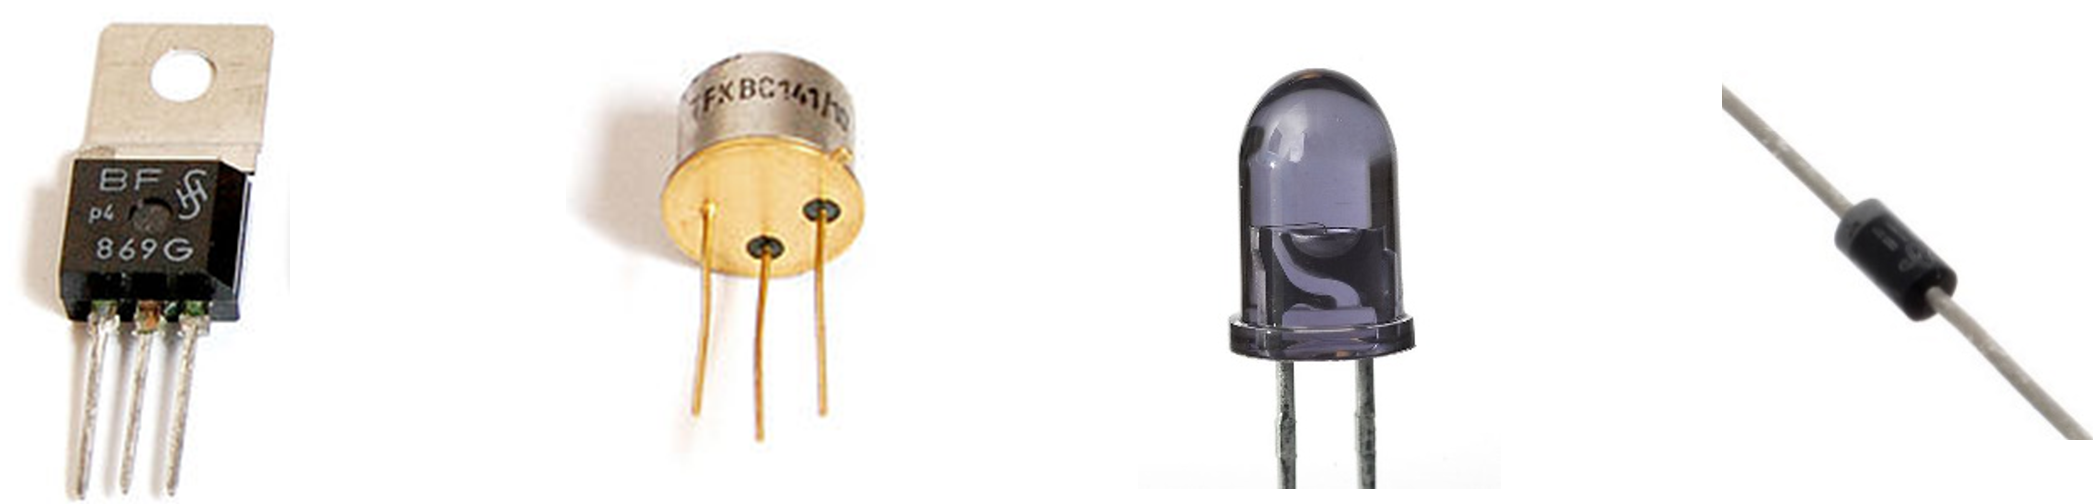
\includegraphics[width=.8\textwidth]{Bilder/kap1/AufnahmenHalbleiterWiki.png}
        %\caption{\textbf{Beispielfotos typischer Halbleiterbauelemente.} V.l.n.r.: Feldeffekttransistor, Bipolartransistor, Leuchtdiode, Diode.}  
        %\label{fig:BeispielfotosVerbreiteterHalbleiterbauelemente}
    \end{figure}
     }
    \speech{Einfuehrung}{2}{Zum Einstieg sehen wir hier eine Auswahl typischer Halbleiterbauelemente.
    Von links nach rechts: ein Feldeffekttransistor, ein Bipolartransistor, eine Leuchtdiode und eine klassische Diode.
    Diese Bauelemente stecken in nahezu jedem elektronischen Gerät - und basieren alle auf denselben physikalischen Prinzipien, die wir uns jetzt nach und nach anschauen.}
\end{frame}

\begin{frame}
\b{\fta{Einführung}
\begin{itemize}
    \item Halbleiterbauelemente sind zentral für die Funktion zahlreicher elektronischer Geräte wie Computer, Mobiltelefone und Solarzellen.
    \item Sie basieren auf Materialien, die weder gute Leiter noch gute Isolatoren sind. Ihre Funktionsweise kann mithilfe des Bändermodells erklärt werden.
    \item In diesem Kapitel werden die Grundlagen der Halbleitertechnik erläutert.
\end{itemize}}
\speech{Einfuehrung}{3}{Halbleiter sind die Grundlage moderner Elektronik - vom Smartphone bis zur Solaranlage.
Sie haben eine besondere Eigenschaft: Sie liegen in ihrer Leitfähigkeit genau zwischen Leitern und Isolatoren.
Und wie lässt sich dieses Verhalten erklären?
Mit dem Bändermodell, das uns zeigt, welche Energiezustände Elektronen in einem Material einnehmen dürfen - und welche nicht.}
\end{frame}

%Zusammenhang Bohrsche Atommodell und Bändermodell.
\newvideofile{Baendermodell}{Bändermodell}
\begin{frame}
\b{\begin{columns}
    \frametitle{Das Bändermodell}
    \column[c]{0.3\textwidth}
    \begin{figure}[H]
        \onslide<1->{
        \begin{minipage}[t]{0.48\textwidth}
            \begin{figure}[H]
                \centering
                \includesvg[width=1\textwidth]{Bilder/kap1/ZusammenhangBohrscheAtommodellundBaendermodell/ZusammenhangBohrscheAtommodellundBaendermodell_1}
            \end{figure}
        \end{minipage}
} \onslide<2->{
        \begin{minipage}[b]{0.48\textwidth}
                \begin{figure}[H]
                \centering
                \includesvg[width=1.1\textwidth]{Bilder/kap1/ZusammenhangBohrscheAtommodellundBaendermodell/ZusammenhangBohrscheAtommodellundBaendermodell_2}
            \end{figure}
        \end{minipage}
}
        %\caption{\textbf{Zusammenhang zwischen dem Bohrschen Atommodell und Bändermodell.} Darstellung des Zusammenhangs 
                %zwischen dem Abstand von Elektronen zum Kern und Höhe des zugehörigen diskreten Energieniveau. Links: Bohrsche 
                %Atommodell eines Si-Atoms. Rechts: Bändermodell eines Si-Atoms mit den möglichen Energieniveaus.}  
        %\label{fig:ZusammenhangBohrschesAtommodellUndBaendermodell}
    \end{figure}
    \column[c]{0.6\textwidth}
        \begin{itemize}
            \onslide<1->{
            \item Das Bändermodell beschreibt die elektronischen Eigenschaften von Festkörpern und ordnet die Energiezustände von Elektronen in Energiebänder.}
            \onslide<2->{
            \item Es hilft, elektrische, optische und magnetische Eigenschaften von Materialien zu verstehen und zu erklären.}
            \onslide<3->{
            \item Das Modell ermöglicht die Erklärung von Leitung, Isolation, Halbleiterverhalten sowie Oberflächen- und Grenzflächenzuständen.}
            \onslide<4->{
            \item In der Abbildung auf der linken Seite ist der Zusammenhang zwischen bohrschem Atommodell und Bändermodell illustriert.}  
        \end{itemize}
    \end{columns}
}
\speech{Baendermodell}{1}{Links sehen wir das Bohrsche Atommodell, das du vielleicht noch aus der Schule kennst:
Elektronen kreisen in definierten Bahnen - oder Schalen - um den Atomkern.
Jede dieser Schalen hat ein festes Energieniveau.
Rechts daneben sehen wir die Entsprechung im Bändermodell:
Auch hier geht es um mögliche Energieniveaus - aber jetzt denken wir nicht mehr an einzelne Bahnen, sondern an Energiezonen im Material, die später zu Bändern zusammengefasst werden.}

\end{frame}

%UebergangVonEnergieniveausZuBaendern
\begin{frame}
    \b{
    \frametitle{Das Bändermodell}
    \begin{figure}[H]
        \centering
        \includesvg[width=\textwidth]{Bilder/kap1/UebergangVonEnergieniveausZuBaendern}
        \caption{\textbf{Übergang von Energieniveaus zu Bändern} Zusammenhang zwischen den möglichen Energiezustände in Abhängigkeit zur Anzahl der Atome. V.l.n.r. Energiezustände von Elektronen bei einem Einzelatom, 2 Atomen (Molekül) und einem Festkörper.}  
        %\label{fig:UebergangVonEnergieniveausZuBaendern}
    \end{figure}

    }
    \speech{Baendermodell}{2}{Jetzt gehen wir einen Schritt weiter.
    Ein einzelnes Atom hat klar definierte Energieniveaus - das sehen wir links.
    Kommen zwei Atome zusammen, wirken sie elektrisch aufeinander.
    Nach dem Pauli-Prinzip dürfen zwei Elektronen nicht denselben Zustand einnehmen - ihre Energieniveaus verschieben sich also leicht voneinander.
    Je mehr Atome beteiligt sind, desto mehr dieser leicht verschobenen Niveaus entstehen.
    Im Festkörper - ganz rechts - gibt es dann so viele solcher Zustände, dass sie praktisch ein Kontinuum bilden.
    Und dieses Kontinuum nennen wir ein Energieband.}
\end{frame}

%Bändermodell Eines Materials bei 0K
\begin{frame}
    \b{
    \frametitle{Einteilung von Materialien}
    \begin{figure}[H]
        \centering
        \includesvg[width=\textwidth]{Bilder/kap1/BaendermodelleinesMaterialsbei0K}
        \caption{\textbf{Bändermodell eines Materials bei 0 K} Darstellung der Energiebänder mit zugehöriger Beschriftung sowie deren alternativen Bezeichnungen.}  
        %\label{fig:BandermodellEinesMaterialsBei0K}
    \end{figure}
    }
\speech{Einteilung_Materialien}{1}{Was bedeuten jetzt die Begriffe Valenzband, Leitungsband und Bandlücke?
Das Valenzband ist der Bereich, in dem Elektronen noch fest an die Atome gebunden sind - sie tragen also nicht zur elektrischen Leitung bei.
Das Leitungsband dagegen ist der Bereich, in dem sich Elektronen frei durch das Material bewegen können - das ist entscheidend für den Stromfluss.
Und dazwischen liegt oft eine sogenannte Bandlücke - also ein Energiebereich, in dem sich keine Elektronen aufhalten können.
Die Größe dieser Lücke entscheidet darüber, ob ein Material ein Leiter, ein Halbleiter oder ein Isolator ist.}
\end{frame}

%Bändermodell verschiedener Halbleitermaterialien
\begin{frame}
    \b{
    \frametitle{Einteilung von Materialien}
    \begin{figure}[H]
        \centering
        \includesvg[width=\textwidth]{Bilder/kap1/BaendermodellverschiedenerMaterialien}
        \caption{\textbf{Bändermodell verschiedener Halbleitermaterialien} V.l.n.r.: Leiter ohne und mit Überlappung, Halbleiter und Isolator}  
        %\label{fig:BaendermodellVerschiedenerMaterialien}
    \end{figure}
    }
\speech{Einteilung_Materialien}{2}{In der nächsten Abbildung sehen wir, wie sich Materialien anhand ihrer Bandstruktur unterscheiden.
Links: Leiter - hier liegen Valenz- und Leitungsband direkt aneinander oder überlappen sogar.
Elektronen können also ohne großen Energieaufwand ins Leitungsband gelangen - der Strom fließt leicht.
In der Mitte: der Halbleiter - hier gibt es eine kleine Bandlücke, etwa ein Elektronenvolt.
Elektronen brauchen etwas Energie, zum Beispiel durch Erwärmung, um den Sprung ins Leitungsband zu schaffen.
Und ganz rechts: der Isolator - hier ist die Bandlücke sehr groß, typischerweise über 3 Elektronenvolt.
Der Energieaufwand, um ein Elektron ins Leitungsband zu bringen, ist hier so hoch, dass praktisch kein Strom fließt.}
\end{frame}

%Merke
\begin{frame}
    \b{
    \frametitle{Einteilung von Materialien}
    \textbf{Merke:}
    \begin{itemize}
        \onslide<1->{
        \item Ladungsträger können nur definierte Energieniveaus im Festkörper besetzen.
        }
        \onslide<2->{
        \item Bei $T=\mathrm{0\,K}$ ist das Valenzband das höchste besetzte Energieniveau, das darüberliegende Leistungsband beinhaltet keine freien Ladungsträger.
        }
        \onslide<3->{
        \item Materialien können über die Bandlücke Kategorisiert werden. 
        }
    \end{itemize}}
    \speech{Einteilung_Materialien}{3}{Merken wir uns:
    Nur Elektronen im Leitungsband können sich frei durch das Material bewegen - und damit Strom leiten.
    Ob ein Stoff ein Leiter, Halbleiter oder Isolator ist, hängt also direkt von der Größe der Bandlücke ab.
    Ladungsträger können nur definierte Energieniveaus im Festkörper besetzen.
    Bei T = 0 Kelvin ist das Valenzband das höchste besetzte Energieniveau, das darüberliegende Leistungsband beinhaltet keine freien Ladungsträger.
    Materialien können über die Bandlücke Kategorisiert werden}
\end{frame}


%Diamant-Gitterstruktur von Silizium
\begin{frame}
    \b{
    \frametitle{Halbleitermaterialien}
    \begin{figure}[H]
        \centering
        \includesvg[width=0.4\textwidth]{Bilder/kap1/Gitterstrukturen/GitterSi}
        %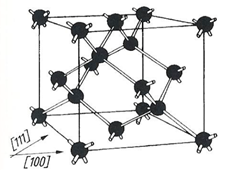
\includegraphics[width=0.5\textwidth]{Bilder/kap1/Diamant-GitterstrukturVonSilizium.png}
        \caption{\textbf{Diamantgitterstruktur von Silizium}}  
        %\label{fig:Diamant-GitterstrukturVonSilizium}
    \end{figure}
    }
    \speech{Halbleitermaterialien}{1}{In diesem Abschnitt schauen wir uns an, wie Halbleitermaterialien aufgebaut sind - und wie man ihre Leitfähigkeit gezielt beeinflussen kann.
    Den Anfang macht das Siliziumgitter.
    Silizium kristallisiert in einer sogenannten Diamantgitterstruktur.
    Das heißt: Jedes Siliziumatom ist tetraedrisch von vier weiteren Atomen umgeben.
    Diese Anordnung sorgt für eine hohe mechanische Stabilität - und gleichzeitig dafür, dass sich Elektronen in alle Richtungen gut bewegen können.
    Ein weiterer Vorteil: Die Struktur ist dreidimensional sehr regelmäßig, was die Halbleitereigenschaften überhaupt erst möglich macht.}
\end{frame}

%Zinkblende-Gitterstruktur von GaAs
\begin{frame}
    \b{
    \frametitle{Halbleitermaterialien}
    \begin{figure}[H]
        \centering
        %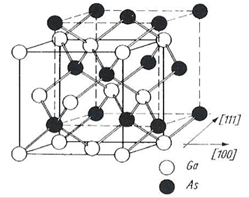
\includegraphics[width=0.5\textwidth]{Bilder/kap1/Zinkblende-GitterstrukturVonGaAs.png}
        \begin{minipage}[c]{0.48\textwidth}
            \centering
            \includesvg[width=0.7\textwidth]{Bilder/kap1/Gitterstrukturen/GitterGaAs_1}
        \end{minipage}
        \begin{minipage}[c]{0.48\textwidth}
            \centering
            \includesvg[width=0.7\textwidth]{Bilder/kap1/Gitterstrukturen/GitterGaAs_2}
        \end{minipage}
        \caption{\textbf{Zinkblende-Gitterstruktur von GaAs}}  
        %\label{fig:Zinkblende-GitterstrukturVonGaAs}
    \end{figure}
    }
    \speech{Halbleitermaterialien}{2}{Ein anderes Beispiel ist Galliumarsenid - ein sogenannter Verbindungshalbleiter.
    Er besteht aus zwei verschiedenen Elementen: Gallium aus der dritten Hauptgruppe und Arsen aus der fünften Hauptgruppe.
    Diese beiden bilden gemeinsam eine Zinkblende-Gitterstruktur - die zwar ähnlich aussieht wie beim Silizium, aber regelmäßig zwischen zwei Atomarten wechselt.
    Diese Kombination sorgt für besondere elektronische Eigenschaften - etwa eine kleinere Bandlücke und gute optische Eigenschaften.
    Deshalb wird Galliumarsenid oft in L E Ds, Laserdioden oder Hochfrequenz-Schaltungen eingesetzt.}
\end{frame}

%Merke
\begin{frame}
    \b{
    \frametitle{Halbleitermaterialien}
    \textbf{Merke:}
    \begin{itemize}
        \onslide<1->{
        \item Silizium ist das am weitesten verbreitete Halbleitermaterial.
        }
        \onslide<2->{
        \item Verbindungshalbleiter bestehen aus zwei Materialen die in bestimmter Kombination Halbleiterverhalten aufweisen.
        }
        \onslide<3->{
        \item Silizium ist aus der IV. Hauptguppe des Periodensystem, Verbindungshalbleiter typischerweise aus der III. und V. Hauptguppe.
        }
    \end{itemize}}
    \speech{Halbleitermaterialien}{3}{Was solltest du dir merken?
Silizium, aus der vierten Hauptgruppe, ist das am häufigsten genutzte Halbleitermaterial - weil es kostengünstig, verfügbar und gut verarbeitbar ist.
Verbindungshalbleiter wie Galliumarsenid bestehen dagegen aus Elementen unterschiedlicher Hauptgruppen, oft der dritten und fünften.
Erst ihre spezielle Kombination ergibt ein stabiles Gitter mit Halbleitereigenschaften.}
\end{frame}

%Tabelle Halbleiter Folie 1
\begin{frame}
    \b{
        \frametitle{Halbleitermaterialien}
        \begin{table}[H]
            \centering 
            \begin{tabular}{|p{1.7cm}|p{1.2cm}|p{2cm}|p{2.2cm}|p{2.2cm}|p{2.3cm}|}
                \hline
                \textbf{Material} & \textbf{Band- \newline lücke \newline (eV)} & \textbf{Ladungs- \newline trägerdichte \newline (cm$^{-3}$)} & \textbf{Elektronen- \newline beweglichkeit \newline (cm$^2$/Vs)} & \textbf{Löcher- \newline beweglichkeit \newline (cm$^2$/Vs)} & \textbf{Anwendungen}\\
                \hline
                Si  & 1,1 & $10^{10} - 10^{15}$ & 1500 & 450 & Mikrochips, \newline Solarzellen, Sensoren \\
                \hline
                Ge & 0,7 & $10^{13} - 20^{19}$ & 3900 & 1900 & Transistoren, \newline Infarot-Detektoren \\
                \hline
                GaAs & 1,43 & $10^6 - 10^8$ & 8500 & 400 & Hochfrequenz- schaltungen, LEDs, Laserdioden \\
                \hline
                \end{tabular}
                \caption{Eigenschaften verschiedener Halbleitermaterialien}
                %\label{tab:EigenschaftenVerschiedenerHalbleitermaterialien}
        \end{table}
    }

    %Gesprochener Text:
    %%
\end{frame}

%Tabelle Halbleiter Folie 1
\begin{frame}
    \b{
        \frametitle{Halbleitermaterialien}
        \begin{table}[H]
            \centering 
            \begin{tabular}{|p{1.7cm}|p{1.2cm}|p{2cm}|p{2.2cm}|p{2.2cm}|p{2.3cm}|}
                \hline
                \textbf{Material} & \textbf{Band- \newline lücke \newline (eV)} & \textbf{Ladungs- \newline trägerdichte \newline (cm$^{-3}$)} & \textbf{Elektronen- \newline beweglichkeit \newline (cm$^2$/Vs)} & \textbf{Löcher- \newline beweglichkeit \newline (cm$^2$/Vs)} & \textbf{Anwendungen}\\
                \hline
                InP & 1,35 & $10^{16} - 10^{17}$ & 5000 - 7000 & 200 - 400 & Optoelektronik, \newline Solarzellen \\
                \hline 
                GaN & 3,4 & $10^{13} - 10^{17}$ & 1000 - 2000 & 50- 200 & Leistungs- \newline elektronik, LED-Beleuchtung, Displays \\
                \hline
                SiC & 3,0 & $10^{12} - 10^{16}$ & 800 - 1200 & 200 - 400 & Leistungs- \newline eletronik, \newline Hochtemperatur- \newline anwendung \\ 
                \hline
                \end{tabular}
                \caption{Eigenschaften verschiedener Halbleitermaterialien}
                %\label{tab:EigenschaftenVerschiedenerHalbleitermaterialien}
        \end{table}
    }
    \speech{Halbleitermaterialien}{4}{Diese Tabellen geben dir einen Überblick über verschiedene Halbleitermaterialien - mit ihren physikalischen Eigenschaften und typischen Anwendungen.
    Wir gehen hier nicht auf jede Zahl ein, aber ein paar Punkte stechen heraus:

    Silizium mit eins Komma eins Elektronenvolt Bandlücke ist der Standard für Mikroelektronik - universell einsetzbar.

    Galliumarsenid hat eine hohe Elektronenbeweglichkeit - deshalb ideal für hohe Frequenzen.

    Gallium-Nitrid und Siliziumcarbid haben eine sehr große Bandlücke - das macht sie perfekt für die Leistungselektronik oder Anwendungen mit hoher Temperatur oder Spannung.

    Wichtig: Je nach Anwendung spielt nicht nur die Bandlücke eine Rolle, sondern auch, wie gut sich Elektronen und sogenannte Löcher im Material bewegen können.}
    

    %Gesprochener Text:
    %%
\end{frame}

%Gitterstruktur und Bändermodell von Si - Abbildung 8
\newvideofile{Ladungstraegertransport}{Ladungsträgertransport}
\begin{frame}
    \b{
    \frametitle{Ladungsträgertransport}
    \onslide<1->{
    \begin{minipage}[t]{0.48\textwidth}
        \begin{figure}[H]
            \centering
            \includesvg[width=\textwidth]{Bilder/kap1/GitterstrukturUndBaendermodellVonSi/GitterstrukturUndBaendermodellVonSi_1}
            \caption{\textbf{Gitterstruktur und Bändermodell von Si} reines Silizium bei T $=$ 0 K}  
            \label{fig:GitterstrukturUndBaendermodellVonSi-1}
        \end{figure}
    \end{minipage}
    }
    \onslide<2->{
    \begin{minipage}[t]{0.48\textwidth}
        \begin{figure}[H]
            \centering
            \includesvg[width=\textwidth]{Bilder/kap1/GitterstrukturUndBaendermodellVonSi/GitterstrukturUndBaendermodellVonSi_2}
            \caption{\textbf{Gitterstruktur und Bändermodell von Si} reines Silizium bei T $>$ 0 K}  
            \label{fig:GitterstrukturUndBaendermodellVonSi-2}
        \end{figure}
    \end{minipage}
    }
    }
    \speech{Ladungstraegertransport}{1}{Und wie kommt Bewegung in die Sache?
    Schauen wir uns das Verhalten von reinem Silizium bei verschiedenen Temperaturen an.
    Links: Bei 0 Kelvin ist das Valenzband voll, das Leitungsband leer - das heißt: Keine freien Ladungsträger, kein Stromfluss.
    Rechts: Steigt die Temperatur, erhalten manche Elektronen genug Energie, um in das Leitungsband zu springen.
    Dort sind sie frei beweglich - und zurück bleibt ein Loch im Valenzband, das ebenfalls als positiver Ladungsträger wirkt.
    So entsteht ein Strom - ganz ohne zusätzliche Dotierung.}
\end{frame}

%Gitterstruktur und Bändermodell von n-dotiertem Si - Abbildung 9
\begin{frame}
    \b{\frametitle{Ladungsträgertransport}
    \onslide<1->{
        \begin{minipage}[t]{0.48\textwidth}
            \begin{figure}[H]
                \centering
                \includesvg[width=\textwidth]{Bilder/kap1/GitterstrukturUndBaendermodellVonN-dotiertesSi/GitterstrukturUndBaendermodellVonN-dotiertesSi_1}
                \caption{\textbf{Gitterstruktur und Bändermodell von n-dotiertem Si} n-dotierts Silizium bei T $=$ 0 K.}  
                \label{fig:GitterstrukturUndBaendermodellVonN-DotiertesSi-1}
            \end{figure}
        \end{minipage}
    }
    \onslide<2->{
        \begin{minipage}[t]{0.48\textwidth}
            \begin{figure}[H]
                \centering
                \includesvg[width=\textwidth]{Bilder/kap1/GitterstrukturUndBaendermodellVonN-dotiertesSi/GitterstrukturUndBaendermodellVonN-dotiertesSi_2}
                \caption{\textbf{Gitterstruktur und Bändermodell von n-dotiertem Si} n-dotierts Silizium bei T $>$ 0 K.}  
                \label{fig:GitterstrukturUndBaendermodellVonN-DotiertesSi-2}
            \end{figure}
        \end{minipage}
    }
    }
    \speech{Ladungstraegertransport}{2}{Noch effektiver wird es durch Dotierung.
    Bei der sogenannten n-Dotierung wird zum Beispiel Phosphor eingebracht - ein Element mit fünf Valenzelektronen, eines mehr als Silizium.
    Dieses zusätzliche Elektron ist nur locker gebunden und sitzt in einem Donator-Niveau, knapp unter dem Leitungsband.
    Links: Bei 0 Kelvin bleibt es noch dort - aber rechts sehen wir: Schon bei leicht erhöhter Temperatur kann es ins Leitungsband springen.
    Damit steht sofort ein freies Elektron für den Stromtransport zur Verfügung.
    Durch diese gezielte Veränderung steigt die Leitfähigkeit deutlich.}
\end{frame}

%Gitterstruktur und Bändermodell von p-dotiertem Si
\begin{frame}
    \b{\frametitle{Ladungsträgertransport}
    \onslide<1->{
    \begin{minipage}[t]{0.48\textwidth}
        \begin{figure}[H]
            \centering
            \includesvg[width=\textwidth]{Bilder/kap1/GitterstrukturUndBaendermodellVonP-dotiertesSi/GitterstrukturUndBaendermodellVonP-dotiertesSi_1}
            \caption{\textbf{Gitterstruktur und Bändermodell von p-dotiertem Si} p-dotierts Silizium bei T $=$ 0 K.}  
            \label{fig:GitterstrukturUndBaendermodellVonP-DotiertesSi-1}
        \end{figure}
    \end{minipage}
    }
    \onslide<2->{
    \begin{minipage}[t]{0.48\textwidth}
        \begin{figure}[H]
            \centering
            \includesvg[width=\textwidth]{Bilder/kap1/GitterstrukturUndBaendermodellVonP-dotiertesSi/GitterstrukturUndBaendermodellVonP-dotiertesSi_2}
            \caption{\textbf{Gitterstruktur und Bändermodell von p-dotiertem Si} p-dotierts Silizium bei T $>$ 0 K.}  
            \label{fig:GitterstrukturUndBaendermodellVonP-DotiertesSi-2}
        \end{figure}
    \end{minipage}
    }
    }
    \speech{Ladungstraegertransport}{3}{Bei der p-Dotierung funktioniert es umgekehrt.
    Hier wird etwa Bor eingebracht - das hat nur drei Valenzelektronen.
    Dadurch fehlt ein Elektron für die Bindung - es entsteht ein sogenanntes Loch, also ein leerer Platz im Valenzband.
    Links: Bei 0 Kelvin bleibt das System unbewegt.
    Rechts: Bei höherer Temperatur kann ein Elektron aus der Umgebung in dieses Loch springen.
    Zurück bleibt - wieder - ein Loch, das sich durch das Material bewegen kann und den Stromtransport in positiver Richtung ermöglicht.}
\end{frame}

%Merke
\begin{frame}
    \b{
    \frametitle{Ladungsträgertransport}
    \textbf{Merke:}
    \begin{itemize}
        \onslide<1->{
        \item Durch thermische Anregung können freie Elektronen entstehen, die zum Ladungsträgertransport beitragen. 
        } \onslide<2->{
        \item Dotierung ist das gezielte Einbringen von Fremdatomen mit oder weniger Valenzelektronen als das Ausgangsmaterial.
        } \onslide<3->{
        \item Für n-Dotierung kann Phosphor und für p-Dotierung Bor genutzt werden.
        }
    \end{itemize}}
    \speech{Ladungstraegertransport}{4}{Zusammengefasst:

    Temperatur kann Elektronen anregen - aber noch viel gezielter funktioniert das durch Dotierung.

    Dabei bringt man Atome mit mehr oder weniger Valenzelektronen ins Gitter ein.

    Für n-Dotierung nimmt man zum Beispiel Phosphor, für p-Dotierung Bor.
    So lässt sich die elektrische Leitfähigkeit von Halbleitern ganz gezielt einstellen.}
\end{frame}

%Driftstrom Innerhalb Eines Halbleiters
\begin{frame}
    \b{
    \frametitle{Ladungsträgertransport}
    \begin{figure}[H]
        \centering
        \includesvg[width=0.5\textwidth]{Bilder/kap1/DriftstromInnerhalbEinesHalbleiters}
        \caption{\textbf{Driftstrom innerhalb eines Halbleiters}}  
        %\label{fig:DriftstromInnerhalbEinesHalbleiters}
    \end{figure}
    }
    \speech{Ladungstraegertransport}{5}{In diesem Video schauen wir uns an, wie sich Ladungsträger in Halbleitern bewegen - und was im sogenannten pn-Übergang passiert.
    Fangen wir mit dem Driftstrom an.
    Wenn wir ein elektrisches Feld anlegen, spüren die freien Ladungsträger im Halbleiter - also Elektronen und Löcher - eine Kraft.
    Elektronen driften dann zur positiven Elektrode, Löcher in die entgegengesetzte Richtung.
    In der Abbildung siehst du: Die Bewegung hängt von der Stärke des Feldes und der Beweglichkeit der Teilchen ab.
    Aber: Das ist nur ein Teil der Geschichte.}
\end{frame}

%Diffusions Innerhalb Eines Halbleiters
\begin{frame}
    \b{
    \frametitle{Ladungsträgertransport}
    \begin{figure}[H]
        \centering
        \includesvg[width=0.8\textwidth]{Bilder/kap1/DiffusionsstromInnerhalbEinesHalbleiters}
        \caption{\textbf{Diffusionsstrom innerhalb eines Halbleiters}}  
        %\label{fig:DiffusionsstromInnerhalbEinesHalbleiters}
    \end{figure}
    }
    \speech{Ladungstraegertransport}{6}{Der zweite wichtige Stromanteil ist der Diffusionsstrom.
    Er entsteht ganz ohne äußeres Feld - nämlich dann, wenn es einen Konzentrationsunterschied gibt.
    Freie Elektronen bewegen sich von Bereichen mit hoher Konzentration zu Bereichen mit niedriger - genauso wie bei der Diffusion von Tinte in Wasser.
    In einem n-dotierten Material bedeutet das: Elektronen wandern dorthin, wo es weniger von ihnen gibt - das ist der Diffusionsstrom.
    Und für Löcher im p-Material gilt genau das Gleiche - nur eben umgekehrt.}
\end{frame}

%Einfluss von Spannungen auf Halbleiter
\begin{frame}
    \b{
    \frametitle{Ladungsträgertransport}
    \begin{figure}[H]
        \centering
        \includesvg[width=0.8\textwidth]{Bilder/kap1/EinflussvonSpannungenaufHalbleiter}
        \caption{\textbf{Einfluss von Spannungen auf Halbleiter}}  
        %\label{fig:EinflussVonSpannungenAufHalbleiter}
    \end{figure}
    }
    \speech{Ladungstraegertransport}{7}{Und was passiert, wenn wir eine Spannung anlegen?
    Dann verschieben sich die Energiebänder im Halbleiter.
    Ohne Spannung - links in der Abbildung - sind die Bänder horizontal, es fließt kein Strom.
    Mit Spannung - rechts - entsteht eine Schräglage der Bänder:
    Elektronen streben von hoher zu niedriger Energie - es kommt zum Stromfluss.
    Auch hier wirken Drift und Diffusion wieder zusammen.}
\end{frame}

%Merke
\begin{frame}
    \b{
    \frametitle{Ladungsträgertransport}
    \textbf{Merke:}
    \begin{itemize}
        \onslide<1->{
        \item Driftstrom ist der Ladungsträgertransport auf Grund eines elektrischen Feldes.
        } \onslide<2->{
        \item Diffusionsstrom ist die Bewegung von Ladungsträgern auf Grund eines Konzentrationsunterschiedes.
        } \onslide<3->{
        \item Drift- und Diffusionsstrom ergeben zusammen den Gesamtstrom.
        } \onslide<4->{
        \item Eine externe Spannung führt zu einer Verschiebung des Bändermodells. 
        }
    \end{itemize}}
    \speech{Ladungstraegertransport}{8}{Fassen wir kurz zusammen:

    Driftstrom entsteht durch ein elektrisches Feld,
    Diffusionsstrom durch Konzentrationsunterschiede.
    Beide zusammen ergeben den Gesamtstrom.
    Und: Eine angelegte Spannung verändert das Bändermodell - das ist wichtig für das Verhalten im nächsten Teil.}
\end{frame}

\newvideofile{pn-Uebergang}{pn-Übergang}

\begin{frame}
    \b{
    \frametitle{pn-Übergang}
    \begin{figure}[H]
        \centering
        \includesvg[width=\textwidth]{Bilder/kap1/FolienVorgaengeInnerhalbeinesPNUebergangs1}
        \caption{\textbf{Vorgänge innerhalb eines pn-Übergangs.}}  
        %\label{fig:VorgaengeInnerhalbEinesPn-Uebergangs1}  
    \end{figure}
    }
    \speech{pn-Uebergang}{1}{Jetzt kommen wir zum pn-Übergang - einem zentralen Baustein vieler Bauelemente.
    Er entsteht, wenn ein p-dotierter Halbleiter mit einem n-dotierten verbunden wird.
    Links und rechts sehen wir: In beiden Bereichen gibt es freie Ladungsträger - Elektronen und Löcher.
    Aber in der Mitte, an der Grenze, passiert etwas Interessantes.}
\end{frame}

\begin{frame}
    \b{
    \frametitle{pn-Übergang}
    \begin{figure}[H]
        \centering
        \includesvg[width=0.6\textwidth]{Bilder/kap1/FolienVorgaengeInnerhalbeinesPNUebergangs2}
        \caption{\textbf{Vorgänge innerhalb eines pn-Übergangs.} }  
    \end{figure}
          \begin{itemize}
            \onslide<1->{
        \item Durch die Bindung der Löcher und Elektronen an deren Atome begrenzt den Diffusionsstrom.
            } \onslide<2->{
        \item Der Bereich in der Mitte nennt sich Raumladungszone (RLZ). Dort sind keine freien Ladungsträger, da die Elektronen und Löcher sich gegenseitig neutralisieren.
            } \onslide<3->{
        \item Es entsteht ein elektrisches Feld zwischen den p- und n-dotierten Bereichen.
            }
    \end{itemize}
    }
    \speech{pn-Uebergang}{2}{Durch Diffusion wandern Elektronen vom n- ins p-Gebiet, und Löcher vom p- ins n-Gebiet.
    Dabei stoßen sie auf Teilchen mit entgegengesetzter Ladung - und rekombinieren.
    Zurück bleiben ungeladene Atome, die zu geladenen Ionen werden.
    So entsteht in der Mitte eine Zone ohne freie Ladungsträger - die sogenannte Raumladungszone.
    Hier bildet sich ein inneres elektrisches Feld, das eine Art natürliche Sperre bildet.}
\end{frame}

%Vorgänge innerhalb des pn-Übergangs.
\begin{frame}
    \b{
    \frametitle{pn-Übergang}
    \begin{figure}[H]
        \centering
        \includesvg[width=\textwidth]{Bilder/kap1/VorgaengeInnerhalbDesPN-Uebergangs}
        \caption{\textbf{Vorgänge innerhalb des pn-Übergangs.}}  
        %\label{fig:VorgaengeInnerhalbDesPn-Uebergangs}
    \end{figure}
    }
    \speech{pn-Uebergang}{3}{In der Raumladungszone wirken jetzt zwei Kräfte gegeneinander:
    Diffusion möchte weiterhin Ladungsträger nach außen treiben,
    das elektrische Feld erzeugt einen Driftstrom in die entgegengesetzte Richtung.
    Im Gleichgewicht ist beides im Gleichgewicht - es fließt kein Strom, obwohl Ladungsträger vorhanden sind.
    Das macht den pn-Übergang so besonders.}
\end{frame}

%Einfluss von Spannungen auf pn-Übergang.
\begin{frame}
    \b{
    \frametitle{pn-Übergang}
    \begin{figure}[H]
        \centering
        \includesvg[width=0.7\textwidth]{Bilder/kap1/EinflussvonSpannungenaufpn-Uebergang}
        \caption{\textbf{Einfluss von Spannungen auf pn-Übergang.} Raumladungszone bei verschiedenen angelegten Spannungen. Links: Spannung in Durchlassrichtung. Rechts: Spannung entgegen der Durchlassrichtung, Sperrrichtung}  
        %\label{fig:EinflussVonSpannungenAufPn-Uebergang}
    \end{figure}
    }
    \speech{pn-Uebergang}{4}{Was passiert, wenn wir eine äußere Spannung anlegen?
    Links siehst du den Fall einer Durchlassrichtung:
    Die externe Spannung verringert die Barriere - die Raumladungszone wird schmaler, und Strom kann fließen.
    Rechts: Sperrrichtung - die Spannung verstärkt das innere Feld, die Barriere wächst, und der Stromfluss wird unterdrückt.
    Das ist das Prinzip einer Diode - Strom in eine Richtung ja, in die andere nein.}
\end{frame}

%Merke
\begin{frame}
    \b{
    \frametitle{pn-Übergang}
    \textbf{Merke:}
    \begin{itemize}
        \onslide<1->{
        \item Der pn-Übergang kombiniert eine p- und n-dotierte Halbleiterschicht.
        } \onslide<2->{
        \item Im Übergangsbereich sind keine freien Ladungsträger, der Bereich wird Raumladungszone genannt.
        } \onslide<3->{
        \item In Durchlassrichtung wird die RLZ verkleinert, in Sperrrichtung wird diese vergrößert.  
        }
    \end{itemize}}
    \speech{pn-Uebergang}{5}{Was du dir merken solltest:
    Der pn-Übergang ist die Verbindung von p- und n-dotierten Schichten,
    in der Raumladungszone gibt es keine freien Ladungsträger,
    bei Durchlassrichtung wird sie kleiner - bei Sperrrichtung größer.
    Das Verhalten lässt sich durch das Bändermodell und das Wechselspiel aus Drift und Diffusion gut erklären.}
\end{frame}

\s{\fta{Bauelemente}
In den folgenden Abschnitten werden verschiedene Arten von Halbleiterbauelementen genauer betrachtet, 
darunter Dioden, Leuchtdioden (LEDs), Bipolartransistoren und Feldeffekttransistoren. Dabei wird auf 
das elektrische Verhalten, den Aufbau, die wichtigsten Kenngrößen und deren vielfältige Anwendungen eingegangen.

\begin{Lernziele}{Halbleiterbauelemente}
    \title{Lernziele: Halbleiterbauelemente}
    Die Studierenden können
    \begin{itemize}
        \item Bauteile für verschiedene Anwendungen auswählen.
        \item den Aufbau verschiedener Halbleiterbauelemente beschreiben.
        \item Arbeitspunkte bestimmen und fehlende Bauteilwerte berechnen. 
        \item Anwendungen einzelner Bauelemente nennen.
    \end{itemize}
    \end{Lernziele}
}    

%\speech{Bauelemente}{1}{
%    In den folgenden Abschnitten werden verschiedene Arten von Halbleiterbauelementen genauer betrachtet,
%    darunter Dioden, Leuchtdioden (LEDs), Bipolartransistoren und Feldeffekttransistoren. Dabei wird auf
%    das elektrische Verhalten, den Aufbau, die wichtigsten Kenngrößen und deren vielfältige Anwendungen eingegangen.
%}

%\speech{Lernziele}{1}{
%    Die Studierenden können Bauteile für verschiedene Anwendungen auswählen. Sie können den Aufbau verschiedener Halbleiterbauelemente beschreiben und Arbeitspunkte bestimmen. 
%    Sie können fehlende Bauteilwerte berechnen und Anwendungen einzelner Bauelemente nennen.
%}

\s{\ftb{Diode}
Die Diode ist das Halbleiterbauelement mit dem einfachsten Aufbau, bestehend aus nur einem pn-Übergang. Dadurch ergeben sich 
zwei Anschlüsse: Die sogenannte Anode am p-dotierten Bereich und die Kathode am n-dotierten Bereich. Wie bereits 
im Abschnitt 1.4 beschrieben, ermöglicht der pn-Übergang den Stromfluss in nur einer Richtung, weshalb Dioden oft 
zur Gleichrichtung und Spannungsstabilisierung eingesetzt werden.

%Abbildung 16
\begin{figure}[H]
    \begin{minipage}[c]{0.3\textwidth}
        \centering
        \begin{circuitikz}[]
    \draw (0,0) to[D, v>, name=UD] (0,-2);
    \varrmore{UD} {$U_\mathrm{D}$};
\end{circuitikz}
    \end{minipage}
    \begin{minipage}[c]{0.3\textwidth}
        \centering
        \includesvg[width= 0.15\textwidth]{Bilder/kap2/SiliziumDiode/SiliziumDiode2}  
    \end{minipage}
    \begin{minipage}[c]{0.25\textwidth}
        \centering
        \includesvg[width= .8\textwidth]{Bilder/kap2/SiliziumDiode/SiliziumDiode3}
    \end{minipage}
    \label{fig:SiliziumDiode}
    \caption{\textbf{Silizium Diode.} V.l.n.r.: Schaltzeichen, Bauform und Querschnitt einer Silizium Diode.} 
\end{figure}
}
%\speech{Die Abbildung zeigt eine Silizium-Diode in drei verschiedenen Darstellungen:  
%
%Links: Schaltzeichen der Diode
%- Die Diode wird als ein Dreieck mit einer horizontalen Linie dargestellt.  
%- Das Dreieck zeigt in Richtung der Anode, während die Linie die Kathode repräsentiert.  
%- Eine blaue Pfeilmarkierung mit  U D zeigt die Richtung der angelegten Spannung an.  
%- Dieses Symbol wird in Schaltplänen zur Kennzeichnung von Dioden verwendet.  
%
%Mitte: Gehäuseform einer realen Diode
%- Das mittlere Symbol stellt die typische Bauform einer Siliziumdiode dar.  
%- Die Anode befindet sich oben, die Kathode unten.  
%- Die Diode ist als schwarzer, rechteckiger Körper mit zwei Anschlussbeinchen dargestellt.  
%- Ein weißer Balken markiert die Kathodenseite, um die Polung der Diode zu verdeutlichen.  
%
%Rechts: Querschnitt einer Silizium-Diode 
%- Die rechte Darstellung zeigt die innere Struktur der Diode.  
%- Die Diode besteht aus einem Halbleitermaterial (Si für Silizium), das in zwei Bereiche unterteilt ist:  
%  - Ein **p-dotierter Bereich** oben (rot markiert), der als Anode dient.  
%  - Ein **n-dotierter Bereich** unten (blau markiert), der als Kathode dient.  
%- Der Übergang zwischen den beiden Bereichen bildet einen **pn-Übergang**, der für die Gleichrichterfunktion der Diode verantwortlich ist.  
%- Die Anode und Kathode sind jeweils mit elektrischen Anschlüssen verbunden, um den Stromfluss zu ermöglichen.  
%
%Diese Abbildung zeigt die drei wesentlichen Darstellungen einer Siliziumdiode:  
%- Das Schaltzeichen für elektrische Schaltpläne,  
%- Die physische Bauform als reales Bauteil,  
%- Den inneren Aufbau, der die Funktion als Halbleiterbauelement ermöglicht.  
%
%Siliziumdioden werden häufig zur Gleichrichtung von Wechselstrom, Spannungsstabilisierung und Schutzschaltungen eingesetzt.}


%\speech{Diode}{1}{
%    Die Diode ist das Halbleiterbauelement mit dem einfachsten Aufbau, bestehend aus nur einem pn-Übergang. Dadurch ergeben sich
%    zwei Anschlüsse: die sogenannte Anode am p-dotierten Bereich und die Kathode am n-dotierten Bereich. Wie bereits
%    im Abschnitt 1.4 beschrieben, ermöglicht der pn-Übergang den Stromfluss in nur einer Richtung, weshalb Dioden oft
%    zur Gleichrichtung und Spannungsstabilisierung eingesetzt werden.
%   Abbildung 2.1 zeigt das Schaltzeichen, die Bauform und den Querschnitt einer Siliziumdiode.
%}


\s{\ftc{Elektrisches Verhalten}
\label{sec:ElektrischesVerhalten}
Das elektrische Verhalten von Dioden wird wesentlich durch ihre Kennlinie beschrieben, die stark nichtlinear ist. 
Diese Kennlinie stellt den durch die Diode fließenden Strom in Abhängigkeit von der extern angelegten Spannung dar. 
Charakteristische Bereiche der Kennlinie sind der Durchlass-, Sperr- und Durchbruchbereich.

\begin{itemize}
    \item \textbf{Durchlassbereich:} Vom Betrieb im Durchlassbereich wird gesprochen, wenn eine positive Spannung in Richtung der Diode angelegt wird, 
    also wenn das elektrische Potenzial an der Anode größer ist als das an der Kathode (Bereich rechts von der y-Achse, 
    siehe Abbildung \ref{fig:Diodenkennlinie}). Bei einer Spannung oberhalb der Schleusenspannung ($U_\mathrm{S}$) steigt der Diodenstrom 
    näherungsweise exponentiell an. Die Schleusenspannung ist eine materialspezifische Spannung, die mindestens 
    benötigt wird, um die Raumladungszone so stark zu verringern, dass ein Stromfluss ermöglicht wird. Bei 
    Siliziumdioden liegt diese typischerweise bei ${0,6}$ bis ${0,7}\,\mathrm{V}$.

    \item \textbf{Sperrbereich:} Liegt vor, wenn die angelegte Spannung negativ ist (Bereich links von der y-Achse). 
    In diesem Bereich fließt kaum Strom, da der Widerstand der Diode sehr groß ist.

    \item \textbf{Durchbruchbereich:} Bei einer Spannung unterhalb der Durchbruchspannung ($U_\mathrm{BR}$) kommt es 
    zu einem Durchbruch und es fließt schlagartig ein sehr hoher Strom. Ist die Diode nicht speziell für den Durchbruch 
    ausgelegt, führt der hohe Strom zur Überlastung und folglich zur Zerstörung des Bauelements.

\end{itemize}

%\speech{Elektrisches Verhalten}{1}{
%    Das elektrische Verhalten von Dioden wird wesentlich durch ihre Kennlinie beschrieben, die stark nichtlinear ist.
%    Diese Kennlinie stellt den durch die Diode fließenden Strom in Abhängigkeit von der extern angelegten Spannung dar.
%    Charakteristische Bereiche der Kennlinie sind der Durchlass-, Sperr- und Durchbruchbereich.
%        Durchlassbereich: Vom Betrieb im Durchlassbereich wird gesprochen, wenn eine positive Spannung in Richtung der Diode angelegt wird,
%        also das elektrische Potenzial an der Anode größer ist als das an der Kathode (Bereich rechts von der y-Achse,
%        siehe Abbildung 2.1). Bei einer Spannung oberhalb der Schleusenspannung ($U_\mathrm{S}$) steigt der Diodenstrom
%        näherungsweise exponentiell an. Die Schleusenspannung ist eine materialspezifische Spannung, die mindestens
%        benötigt wird, um die Raumladungszone so stark zu verringern, dass ein Stromfluss ermöglicht wird. Bei
%        Siliziumdioden liegt diese typischerweise bei ${0,6}$ bis ${0,7}\,\mathrm{V}$.
%        Der Sperrbereich liegt vor, wenn die angelegte Spannung negativ ist (Bereich links von der y-Achse).
%        In diesem Bereich fließt kaum Strom, da der Widerstand der Diode sehr groß ist.
%        Durchbruchberei: Bei einer Spannung unterhalb der Durchbruchspannung ($U_\mathrm{BR}$) kommt es
%        zu einem Durchbruch und es fließt schlagartig ein sehr hoher Strom. Ist die Diode nicht speziell für den Durchbruch
%        ausgelegt, führt der hohe Strom zur Überlastung und folglich zur Zerstörung des Bauelements.
%   Abbildung 2.2 zeigt die Diodenkennlinie mit den drei genannten Bereichen.
%}


%Abbildung 17
\begin{figure}[H]
    \centering
    \includesvg[width= 0.6\textwidth]{Bilder/kap2/Diodenkennlinie}
    \caption{\textbf{Diodenkennlinie.} Relevante Bereiche v.l.n.r.: Durchbruchbereich, Sperrbereich und Durchlassbereich.}  
    \label{fig:Diodenkennlinie}
\end{figure}
}
%\speech{Die Abbildung zeigt die Diodenkennlinie, welche das Strom-Spannungs-Verhalten einer Diode beschreibt. Die Darstellung ist in drei farblich gekennzeichnete Bereiche unterteilt:  
%1. Links (rot): Durchbruchbereich
%- Dieser Bereich befindet sich für negative Spannungen, also im Rückwärtsbetrieb der Diode.  
%- Für eine kleine negative Spannung fließt nahezu kein Strom, da die Diode in Sperrrichtung betrieben wird.  
%- Sobald die Spannung den Durchbruchwert \( U_{BR} \) erreicht, steigt der Strom abrupt stark an. Dies geschieht durch den Lawinendurchbruch oder den Zenerdurchbruch, je nach Diodentyp.  
%- Im Diagramm ist dieser Bereich durch einen steilen Abfall des Stroms in den negativen Bereich gekennzeichnet.  
%
%2. Mitte (blau): Sperrbereich
%- Dieser Bereich liegt zwischen \( U_{BR} \) und \( U_S \), also nahe der Nullspannung.  
%- In diesem Bereich befindet sich die Diode im Sperrzustand.  
%- Der Strom ist sehr gering und beträgt nur wenige Nano- oder Mikroampere (Sperrstrom).  
%- Die Kennlinie verläuft hier nahezu horizontal entlang der Spannungsachse, was darauf hinweist, dass die Diode keinen Strom leitet.  
%
%3. Rechts (grün): Durchlassbereich
%- Dieser Bereich beschreibt die Diode im Vorwärtsbetrieb.  
%- Solange die Spannung unterhalb der Schwellenspannung \( U_S \) bleibt, fließt nur ein sehr kleiner Strom.  
%- Ab \( U_S \) steigt der Strom exponentiell an, da die Diode in den leitenden Zustand übergeht.  
%- Dies ist in der Kennlinie als steiler Anstieg nach oben sichtbar.  
%
%Diese Abbildung verdeutlicht das typische Verhalten einer Halbleiterdiode:  
%- Sie sperrt den Stromfluss für negative Spannungen (außer im Durchbruchfall).  
%- Sie leitet erst bei einer bestimmten positiven Spannung \( U_S \), wobei der Strom dann stark anwächst.  
%- Die Kenntnis dieser Kennlinie ist essenziell für das Verständnis und die Anwendung von Dioden in Gleichrichterschaltungen, Spannungsstabilisierungen und Schutzschaltungen.}


\s{Das Ersatzschaltbild einer Siliziumdiode hilft, das Verhalten der Diode in verschiedenen Betriebszuständen besser 
zu verstehen. Es vereinfacht die reale Diode, indem es ihre wesentlichen Eigenschaften modelliert.}

\s{Komponenten des Ersatzschaltbilds:
\begin{itemize}

    \item \textbf{Ideale Diode (D):} 
    Leitet in Vorwärtsrichtung ohne Spannungsverlust und sperrt in
    Rück\-wärts\-rich\-tung vollständig.
    \item \textbf{Schleusenspannung/Schwellenspannung ($U_\mathrm{S}$/ $U_\mathrm{T0}$):} 
    Diese Spannung ist der Wert, bei dem ein messbarer Stromfluss durch die reale Diode vorliegt. 
    Im Ersatzschaltbild wird diese durch eine ideale Spannungsquelle dargestellt. 
    \item \textbf{Differenzieller Widerstand ($r_\mathrm{D}$):}
    Der differenzielle Widerstand ($r_\mathrm{D}$) beschreibt den Widerstand der Diode im Durchlassbereich. 
    Er ist definiert als die Änderung der Spannung ($\Delta u_\mathrm{D}$) geteilt durch die Änderung des Stroms 
    ($\Delta i_\mathrm{D}$) und modelliert die Nichtlinearität der Diode nach dem Erreichen der Schleusenspannung. 
    
\end{itemize} 

\begin{equation}
    r_D = \frac{\Delta u_\mathrm{D}}{\Delta i_\mathrm{D}}
    \label {Formel 1}
\end{equation}

  

%Abbildung 18
\begin{figure}[H]
    \centering
    \begin{minipage}[c]{0.45\textwidth}
        \centering
        \includesvg[width= \textwidth]{Bilder/kap2/DiodenkennlinieUndErsatzschaltbild/DiodenkennlinieUndErsatzschaltbild1}
    \end{minipage}
    \begin{minipage}[c]{0.45\textwidth}
        \centering
        \begin{circuitikz}    
    \draw (0,0) 
        to[short, o-] (1,0)
        to[D = $D$] (2.5,0) 
        to[V, v>, name=U1] (4,0)
        to[R=$r_\mathrm{D}$] (5.5,0)
        to[short ,i, name=out, -o] (6.5 ,0);
    
    \iarrmore {out} {$i_\mathrm{D}$};
    
    \draw (0,-1) to[open,v>, name=Uv] (6.5,-1);
    \varrmore{Uv}{$U_\mathrm{D}$};
    \varrmore{U1}{$U_\mathrm{S}$};
    
\end{circuitikz}
    \end{minipage}
    \caption{\textbf{Diodenkennlinie und Ersatzschaltbild.} Links: Diodenkennlinie mit Näherung für den differenziellen
        Widerstand. Rechts: Diodenersatzschaltbild mit der idealen Diode, Spannungsquelle und differenziellem Widerstand.}
    \label{fig:DiodenkennlinieUndErsatzschaltbild}
\end{figure}
} 

%\speech{Die Abbildung zeigt die Diodenkennlinie mit einer Näherung für den differentiellen Widerstand sowie das zugehörige Ersatzschaltbild einer Diode.  

%Links: Diodenkennlinie mit differentieller Widerstandsnäherung
%- Die Kurve zeigt die typische exponentielle Kennlinie einer Diode mit dem Diodenstrom \( I_D \) auf der vertikalen Achse und der Diodenspannung \( U_D \) auf der horizontalen Achse.  
%- Die Schwellenspannung \( U_S \) ist markiert, ab der die Diode in den leitenden Zustand übergeht.  
%- Im Bereich oberhalb von \( U_S \) ist eine Tangente eingezeichnet, die die lokale Steigung der Kennlinie im sogenannten Nennpunkt beschreibt.  
%- Die Differenz \( \Delta U_D \) auf der x-Achse und \( \Delta I_D \) auf der y-Achse markieren eine kleine Spannungs- und Stromänderung in der Nähe des Arbeitspunkts.  
%- Der differentielle Widerstand \( r_D \) ergibt sich aus der Steigung der Tangente in diesem Punkt und beschreibt das Verhalten der Diode für kleine Änderungen der Betriebsspannung.  
%
%Rechts: Ersatzschaltbild der Diode
%- Das Schaltbild zeigt eine Modellierung der Diode für kleine Signale.  
%- Die ideale Diode \( D \) ist mit einer Spannungsquelle \( U_S \) in Serie geschaltet.  
%- Zusätzlich ist ein differentieller Widerstand \( r_D \) in Reihe eingefügt, um die dynamische Änderung des Widerstands in Abhängigkeit von der Betriebsspannung zu berücksichtigen.  
%- Der Diodenstrom \( i_D \) fließt durch das gesamte Netzwerk, während \( U_D \) die angelegte Spannung über der Diode darstellt.  
%
%Diese Abbildung verdeutlicht die analytische Beschreibung der Diodenkennlinie sowie die praktische Modellierung durch das Ersatzschaltbild. Die Berücksichtigung des differentiellen Widerstands ist besonders relevant für Anwendungen mit Wechselspannungen oder kleinen Signalamplituden, beispielsweise in Hochfrequenz- und Verstärkerschaltungen.}


%\speech{Ersatzschaltbild}{1}{
%    Das Ersatzschaltbild einer Siliziumdiode hilft, das Verhalten der Diode in verschiedenen Betriebszuständen besser
%    zu verstehen. Es vereinfacht die reale Diode, indem es ihre wesentlichen Eigenschaften modelliert.
%    Komponenten des Ersatzschaltbilds:
%    Ideale Diode: Leitet in Vorwärtsrichtung ohne Spannungsverlust und sperrt in
%    Rückwärtsrichtung vollständig.
%    Schleusenspannung/ Schwellenspannung US/U_{T0}:
%    Diese Spannung ist der Wert, bei dem ein messbarer Stromfluss durch die reale Diode vorliegt.
%    signifikant zu leiten.
%    Im Ersatzschaltbild wird diese durch eine ideale Spannungsquelle dargestellt.
%    Differenzieller Widerstand rD:
%    Der differenzielle Widerstand ($r_\mathrm{D}$) beschreibt den Widerstand der Diode im Durchlassbereich.
%    Er ist definiert als die Änderung der Spannung ($\Delta u_\mathrm{D}$) geteilt durch die Änderung des Stroms
%    ($\Delta i_\mathrm{D}$) und modelliert die Nichtlinearität der Diode nach dem Erreichen der Schleusenspannung.
%    Formel 1 zeigt die Berechnung des differenziellen Widerstands.
%    Abbildung 2.3 zeigt die Diodenkennlinie mit Näherung für den differenziellen
%    Widerstand und das Ersatzschaltbild mit der idealen Diode, Spannungsquelle und differenzieller Widerstand.
%}



\s{
    Die Bestimmung des Arbeitspunktes einer Diode ist ein wichtiger Schritt in der Schaltungsentwicklung, da er den stabilen 
    Betriebszustand der Diode unter Berücksichtigung der angelegten Spannung und des Durchlassstroms definiert. Dabei ist es 
    wichtig, die maximale Verlustleistung der Diode zu beachten, um sicherzustellen, dass sie nicht überhitzt und 
    beschädigt wird. Sowohl grafische als auch mathematische Methoden können zur Bestimmung des Arbeitspunktes verwendet 
    werden. Die grafische Methode basiert auf der Darstellung der Strom-Spannungs-Kennlinie der Diode und der Lastlinie der 
    Schaltung. Der Arbeitspunkt ist der Schnittpunkt dieser beiden Linien. Es kann sowohl der Arbeitspunkt durch den vorgegebenen 
    Widerstand ermittelt werden, als auch der Widerstand auf Basis des gewünschten Arbeitspunktes bestimmt werden. In beiden 
    Fällen sollte der Arbeitspunkt unterhalb der Asymptote für die maximale Verlustleistung der Diode liegen.


%\speech{Arbeitspunkt}{1}{
%    Die Bestimmung des Arbeitspunktes einer Diode ist ein wichtiger Schritt in der Schaltungsentwicklung, da er den stabilen
%    Betriebszustand der Diode unter Berücksichtigung der angelegten Spannung und des Durchlassstroms definiert. Dabei ist es
%    wichtig, die maximale Verlustleistung der Diode zu beachten, um sicherzustellen, dass sie nicht überhitzt und
%    beschädigt wird. Sowohl grafische als auch mathematische Methoden können zur Bestimmung des Arbeitspunktes verwendet
%    werden. Die grafische Methode basiert auf der Darstellung der Strom-Spannungs-Kennlinie der Diode und der Lastlinie der
%    Schaltung. Der Arbeitspunkt ist der Schnittpunkt dieser beiden Linien. Es kann sowohl der Arbeitspunkt durch den vorgegebenen
%    Widerstand ermittelt werden, als auch der Widerstand auf Basis des gewünschten Arbeitspunktes bestimmt werden. In beiden
%    Fällen sollte der Arbeitspunkt unterhalb der Asymptote für die maximale Verlustleistung der Diode liegen.
%    Abbildung 2.4 zeigt die grafische Bestimmung des Arbeitspunktes. Links: Diodenkennlinie (schwarz), Widerstandsgerade (blau) und 
%    Asymptote der maximalen Verlustleistung (rot) der Diode. Rechts: Schaltung der Diode mit Vorwiderstand.
%}

%Abbildung 19
\begin{figure}[H]
    \centering
    \begin{minipage}[c]{0.45\textwidth}
        \centering
        \includesvg[width= \textwidth]{Bilder/kap2/GrafischeBestimmungArbeitspunkt/GrafischeBestimmungArbeitspunkt1}
    \end{minipage}
    \begin{minipage}[c]{0.45\textwidth}
        \centering
        \begin{circuitikz}
    \draw (0,0) to[R=$R$] (4,0)
        to[D, v>, i>, name=D] (4,-3)
        to[short] (0,-3)
        to[V, v<, name=U0] (0,0);
    
    \varrmore {D}{$U_\mathrm{D}$};
    \varrmore {U0}{$U_\mathrm{0}$};
    \iarrmore {D}{$I_\mathrm{D}$};
\end{circuitikz}
    \end{minipage}
    \label{fig:GrafischeBestimmungArbeitspunkt}
    \caption{\textbf{ Grafische Bestimmung des Arbeitspunktes.} Links: Diodenkennlinie (schwarz), Widerstandsgerade (blau) und
        Asymptote der maximalen Verlustleitung (rot) der Diode. Rechts: Schaltung der Diode mit Vorwiderstand.}
\end{figure}
}
%\speech{Die Abbildung zeigt die grafische Bestimmung des Arbeitspunkts einer Diode. Links ist die Diodenkennlinie mit der Widerstandsgeraden dargestellt, rechts das zugehörige Ersatzschaltbild mit Vorwiderstand.  
%
%**Links: Diodenkennlinie und Bestimmung des Arbeitspunkts**  
%- Die schwarze Kurve zeigt die exponentielle Diodenkennlinie, welche den Zusammenhang zwischen der Diodenspannung \( u_F(i_D) \) auf der horizontalen Achse und dem Diodenstrom \( i_D \) auf der vertikalen Achse beschreibt.  
%- Die blaue Gerade stellt die Widerstandsgerade dar, die sich aus dem Vorwiderstand \( R \) ergibt und durch die Gleichung  
 % \[
 % i_D = \frac{U_0 - u_F}{R}
 % \]
 % beschrieben wird.  
%- Der Schnittpunkt zwischen der Kennlinie und der Widerstandsgeraden markiert den Arbeitspunkt der Diode.  
%- Die rote gestrichelte Kurve stellt die maximale Verlustleistung \( P_{V, \max} \) der Diode dar.  
%- Der Arbeitspunkt muss innerhalb dieses Bereichs liegen, um thermische Überlastung der Diode zu vermeiden.  
%
%**Rechts: Ersatzschaltbild der Diode mit Vorwiderstand**  
%- Die Schaltung besteht aus einer Spannungsquelle \( U_0 \), einem Vorwiderstand \( R \) und einer Diode.  
%- Der Widerstand begrenzt den Strom \( I_D \), der durch die Diode fließt.  
%- Die Spannung \( U_D \) fällt über der Diode ab.  
%- Der Vorwiderstand schützt die Diode vor Überstrom und stellt sicher, dass der Arbeitspunkt im sicheren Bereich der Kennlinie bleibt.  
%
%Diese Abbildung zeigt, wie der Arbeitspunkt einer Diode bestimmt werden kann und warum ein Vorwiderstand in vielen Anwendungen erforderlich ist. Die Kombination aus Diodenkennlinie und Widerstandsgerade ermöglicht eine einfache grafische Analyse der Betriebseigenschaften der Diode.}


\s{Die mathematische Methode basiert auf der Lösung von Gleichungen, die den Durchlassstrom der Diode und den Spannungsabfall 
über der Last beschreiben. Der Arbeitspunkt wird durch das Gleichsetzen dieser beiden Ausdrücke bestimmt. Dabei ist es wichtig, 
die maximale Verlustleistung der Diode zu berücksichtigen, um sicherzustellen, dass sie innerhalb ihrer Spezifikationen betrieben wird.}

%\speech{Arbeitspunkt}{1}{
%    Die mathematische Methode basiert auf der Lösung von Gleichungen, die den Durchlassstrom der Diode und den Spannungsabfall
%    über der Last beschreiben. Der Arbeitspunkt wird durch das Gleichsetzen dieser beiden Ausdrücke bestimmt. Dabei ist es wichtig,
%    die maximale Verlustleistung der Diode zu berücksichtigen, um sicherzustellen, dass sie innerhalb ihrer Spezifikationen betrieben wird.
%}

\s{
    \begin{Merksatz}{}
        \begin{itemize}
            \item Die Kennlinie der Diode ist stark nichtlinear.
            \item Das Verhalten der Kennlinie kann in drei Bereichen beschrieben werden: Den Durchbruch-, Sperr- und Durchlassbereich.
            \item Mittels idealer Diode, Spannungsquelle und Widerstand kann die reale Diode in verschiedenen Bereichen angenähert werden.
         \end{itemize}
    \end{Merksatz}
}

%\speech{Merksatz}{1}{
%    Die Kennlinie der Diode ist stark nichtlinear. Das Verhalten der Kennlinie kann in drei Bereichen, den Durchbruch-, Sperr- und Durchlassbereich, beschrieben werden.
%    Mittels idealer Diode, Spannungsquelle und Widerstand kann die reale Diode in verschiedenen Bereichen angenähert werden.
%}

\s{\ftc{Aufbau}
Wie bereits in der Einleitung beschrieben, besteht die Diode in der Regel aus einem einzelnen pn-Übergang. Neben der bisher 
betrachteten einfachen Siliziumdiode gibt es noch zahlreiche weitere Dioden. In diesem Abschnitt wird der bisher betrachtete 
Aufbau mit dem einer Schottky-Diode verglichen. Diese ist sehr verbreitet und kommt ohne pn-Übergang aus.\par
Die pn-Diode besteht aus zwei Halbleiterregionen, nämlich der p-dotierten (positiv geladenen) und der n-dotierten (negativ geladenen) 
Region, die sich an einer gemeinsamen Grenzfläche treffen. Die p-Seite wird als Anode und die n-Seite als Kathode bezeichnet. 
Typischerweise besteht der pn-Übergang aus Silizium oder Germanium. Die Elektronen aus der n-Seite rekombinieren mit den Löchern 
aus der p-Seite an der Grenzfläche, was zur Bildung einer Raumladungszone führt. Diese Raumladungszone bildet die Barriere für den 
Stromfluss in Sperrrichtung.
Eine Schottky-Diode besteht aus einem Metall-Halbleiter-Übergang anstelle eines pn-Übergangs. Bei der Herstellung müssen keine 
verschiedenen Dotierungen eingebracht werden. Ein Aufbringen einer geeigneten Metallschicht reicht bereits aus. Das Halbleitermaterial 
ist typischerweise n-dotiert. Der Übergang zwischen dem Metall und dem Halbleiter bildet eine Schottky-Barriere, die den Stromfluss 
blockiert. Durch eine geeignete Materialkombination kann sich an der Grenzfläche eine Raumladungszone ausbilden, ähnlich wie bei der Siliziumdiode.
Diese Dioden sind für schnelle Schaltvorgänge und einem niedrigen Spannungsabfall in Durchlassrichtung optimiert. 

%\speech{Aufbau}{1}{
%    Wie bereits in der Einleitung beschrieben, besteht die Diode in der Regel aus einem einzelnen pn-Übergang. Neben der bisher 
%    betrachteten einfachen Siliziumdiode gibt es noch zahlreiche weitere Dioden. In diesem Abschnitt wird der bisher betrachtete 
%    Aufbau mit dem einer Schottky-Diode verglichen, diese ist sehr verbreitet und kommt ohne pn-Übergang aus.\par
%    Die pn-Diode besteht aus zwei Halbleiterregionen, nämlich der p-dotierten (positiv geladenen) und der n-dotierten (negativ geladenen) 
%    Region, die sich an einer gemeinsamen Grenzfläche treffen. Die p-Seite wird als Anode und die n-Seite als Kathode bezeichnet. 
%    Typischerweise besteht der pn-Übergang aus Silizium oder Germanium. Die Elektronen aus der n-Seite rekombinieren mit den Löchern 
%    aus der p-Seite an der Grenzfläche, was zur Bildung einer Raumladungszone führt. Diese Raumladungszone bildet die Barriere für den 
%    Stromfluss in Sperrrichtung.
%    Eine Schottky-Diode besteht aus einem Metall-Halbleiter-Übergang anstelle eines pn-Übergangs. Bei der Herstellung müssen keine 
%    verschiedenen Dotierungen eingebracht werden, das Aufbringen einer geeigneten Metallschicht reicht bereits aus. Das Halbleitermaterial 
%    ist typischerweise n-dotiert. Der Übergang zwischen dem Metall und dem Halbleiter bildet eine Schottky-Barriere, die den Stromfluss 
%    blockiert. Durch eine geeignete Materialkombination kann sich an der Grenzfläche eine Raumladungszone ausbilden, ähnlich wie bei der Siliziumdiode.
%    Diese Dioden sind für schnelle Schaltvorgänge und einem niedrigen Spannungsabfall in Durchlassrichtung optimiert. 
%   Abbildung 2.5 zeigt den Aufbau und Vergleich einer klassischen Si-Diode und einer Schottky-Diode.
%}

%Abbildung 20
\begin{figure}[H]
    \centering
    \begin{minipage}[c]{0.49\textwidth}
        \centering
        \includesvg[scale=0.6]{Bilder/kap2/SchichtaufbauVonDioden/SchichtaufbauVonDioden1}
    \end{minipage}
    \begin{minipage}[c]{0.49\textwidth}
        \centering
        \includesvg[scale=0.6]{Bilder/kap2/SchichtaufbauVonDioden/SchichtaufbauVonDioden2}
    \end{minipage}
    
    \label{fig:SchichtaufbauVonDioden}
    \caption{\textbf{Schichtaufbau von Dioden.} Aufbau und Vergleich einer klassischen Si-Diode (links)
        und Schottky-Diode (rechts). Siliziumdioxid ($\mathrm{SiO_2}$) ist ein natürliches Oxid von Silizium und dient zur Isolierung. Aluminium (Al) ist ein typisches Metall für elektrische Kontakte.}
\end{figure}
}
%\speech{Die Abbildung zeigt den Schichtaufbau von Dioden und vergleicht den inneren Aufbau einer klassischen Siliziumdiode (links) mit einer Schottky-Diode (rechts).  
%
%**Oben: Schaltzeichen der Dioden**  
%- Links ist das Standardsymbol einer klassischen pn-Diode mit einer Anode (A) und einer Kathode (K).  
%- Rechts ist das Symbol einer Schottky-Diode, das durch eine gebogene Linie auf der Kathodenseite gekennzeichnet ist, um die Metall-Halbleiter-Kontaktstelle darzustellen.  
%
%**Links: Klassische Siliziumdiode**  
%- Die Anode befindet sich oben, die Kathode unten.  
%- Der Hauptbestandteil der Diode ist ein Silizium-Substrat.  
%- Der obere Bereich besteht aus einem **p\(^+\)**-dotierten Bereich (rot), der für die Injektion von Löchern sorgt.  
%- Darunter liegt das **n-Substrat** (blau), das für die Elektronenleitung sorgt.  
%- Das Material ist mit einer Schicht aus **Siliziumdioxid (SiO\(_2\))** isoliert.  
%- Aluminium (Al) wird als Metallkontakt sowohl für die Anode als auch die Kathode genutzt.  
%
%**Rechts: Schottky-Diode**  
%- Die Struktur ist ähnlich aufgebaut, jedoch gibt es einen wichtigen Unterschied:  
%  - Statt eines pn-Übergangs besitzt die Schottky-Diode einen direkten **Metall-Halbleiter-Kontakt** zwischen dem Aluminium (Al) und dem **n-dotierten Halbleiter**.  
%  - Das untere Substrat ist stärker n-dotiert (**n\(^+\)-Substrat**, dunkelblau), um den Widerstand zu minimieren.  
%  - Durch den Metallkontakt entsteht keine klassische Raumladungszone wie in der pn-Diode, sondern eine **Schottky-Barriere**, die für die Gleichrichtung der Diode verantwortlich ist.  
%
%Diese Abbildung verdeutlicht die strukturellen Unterschiede zwischen einer klassischen pn-Diode und einer Schottky-Diode. Während die klassische Diode einen pn-Übergang nutzt, basiert die Schottky-Diode auf einem Metall-Halbleiter-Übergang, was zu einer niedrigeren Schwellenspannung und schnelleren Schaltzeiten führt. Dies macht Schottky-Dioden besonders für Hochfrequenz- und Leistungselektronikanwendungen geeignet.}

\s{
    \begin{Merksatz}{}
        \begin{itemize}
            \item Schottky-Dioden weisen keinen pn-Übergang auf, sondern einen Schottky-Kontakt.
            \item Bei geeigneter Materialkombination bildet sich zwischen Metall und Halbleiter eine RLZ aus. 
         \end{itemize}
    \end{Merksatz}
}
%\speech{Merksatz}{1}{
%    Schottky-Dioden weisen keinen pn-Übergang auf, sondern einen Schottky-Kontakt. 
% Bei geeigneter Materialkombination bilden sich zwischen Metall und Halbleiter eine Raumladungszone aus.
%}



\s{\ftc{Spezielle Dioden}
\label{sec:SpezielleDioden}
Neben den bisher genannten Dioden gibt es noch eine Vielzahl weiterer Varianten, die durch ihren Aufbau verschiedene 
Eigenschaften aufweisen und entsprechende Anwendungen ermöglichen. Die folgende Tabelle gibt eine Übersicht über typische Dioden.}

%\speech{Spezielle Dioden}{1}{
%    Neben den bisher genannten Dioden gibt es noch eine Vielzahl weiterer Varianten, die durch ihren Aufbau verschiedene
%    Eigenschaften aufweisen und entsprechende Anwendungen ermöglichen. Die folgende Tabelle gibt eine Übersicht über typische Dioden.
%}



\s{\begin{table}[H]
    \centering 
    \begin{tabular}{ |p{2.2cm}|p{1.4cm}|p{3.3cm}|p{2.8cm}|p{3.3cm}| }
        \hline
        \textbf{Bezeichnung} & \textbf{Symbol} & \textbf{Kennlinie} & \textbf{Eigenschaften} & \textbf{Anwendung} \\
        \hline
        Gleich\-richter\-diode  
        &
        \begin{minipage}[t][2.4cm][c]{1.4cm}
            \centering \begin{circuitikz} \draw (0,1) to[D] (0,-1); \end{circuitikz}
        \end{minipage}
        & 
        \begin{minipage}[t][2.4cm][c]{3.3cm}
            \centering \includesvg[width=\textwidth]{kap2/spezielleDiodenÜbersichtVerschiedenerDioden/KennlinieGleichrichterdiode}
        \end{minipage}
        & 
        hoher Durchlassstrom,\newline große Sperrspannung &
        Gleichrichtung\\
        \hline
        Schalt\-diode 
        &
        \begin{minipage}[t][2.4cm][c]{1.4cm}
            \centering \begin{circuitikz} \draw (0,1) to[D] (0,-1); \end{circuitikz}
        \end{minipage}
        & 
        \begin{minipage}[t][2.4cm][c]{3.3cm}
            \centering \includesvg[width= \textwidth]{kap2/spezielleDiodenÜbersichtVerschiedenerDioden/KennlinieSchaltdiode}
        \end{minipage}
        & 
        kleiner Durchlasswiderstand,\newline hoher Sperrwiderstand &
        kleine \newline Umschaltzeiten\\
        \hline
        Schottky\-diode
        &
        \begin{minipage}[t][2.4cm][c]{1.4cm}
            \centering \documentclass{standalone}
\usepackage{circuitikz}

\begin{document}

\begin{circuitikz}[font=\LARGE, european]

\draw (0,0) to[sDo] (2,0);

\end{circuitikz}

\end{document}

        \end{minipage}
        & 
        \begin{minipage}[t][2.4cm][c]{3.3cm}
            \centering \includesvg[width=\textwidth]{kap2/spezielleDiodenÜbersichtVerschiedenerDioden/KennlinieSchottkydiode}
        \end{minipage}
        & 
        kleine Durchlassspannung,\newline kleine Sperrspannung &
        HF-Gleichrichter,\newline Freilaufdiode,\newline Schaltnetzteile\\
        \hline
        Z-Diode
        &
        \begin{minipage}[t][2.4cm][c]{1.4cm}
            \centering \begin{circuitikz} \draw (0,1) to[zD] (0,-1); \end{circuitikz}
        \end{minipage}
        & 
        \begin{minipage}[t][2.4cm][c]{3.3cm}
            \centering \includesvg[width=\textwidth]{kap2/spezielleDiodenÜbersichtVerschiedenerDioden/KennlinieZ-Diode}
        \end{minipage}
        & 
        definierte Durchbruchspannung &
        Stabilisierung \newline von Spannungen,\newline Begrenzung\\
        \hline
        Tunnel\-diode
        &
        \begin{minipage}[t][2.4cm][c]{1.4cm}
            \centering \begin{circuitikz} \draw (0,1) to[tD] (0,-1); \end{circuitikz}
        \end{minipage}
        & 
        \begin{minipage}[t][2.4cm][c]{3.3cm}
            \centering \includesvg[width=\textwidth]{kap2/spezielleDiodenÜbersichtVerschiedenerDioden/KennlinieTunneldiode}
        \end{minipage}
        & 
        negativer differentieller Widerstand &
        Entdämpfung \newline von Schwingkreisen,\newline HF-Oszillator\\
        \hline
        Diac
        &
        \begin{minipage}[t][2.4cm][c]{1.4cm}
            \centering \begin{circuitikz} \draw (0,1) to[biD] (0,-1); \end{circuitikz}
        \end{minipage}
        & 
        \begin{minipage}[t][2.4cm][c]{3.3cm}
            \centering \includesvg[width= \textwidth]{kap2/spezielleDiodenÜbersichtVerschiedenerDioden/KennlinieDiac-Diode}
        \end{minipage}
        & 
        gesteuerter Durchbruch & 
        Entdämpfung,\newline Triggerdiode\\
        \hline
    \end{tabular}
\end{table}
}

\s{\begin{table}[H]
    \centering 
    \begin{tabular}{ |p{2.2cm}|p{1.4cm}|p{3.3cm}|p{2.8cm}|p{3.3cm}| }
        \hline
        \textbf{Bezeichnung} & \textbf{Symbol} & \textbf{Kennlinie} & \textbf{Eigenschaften} & \textbf{Anwendung} \\
        \hline
        Photo\-diode
        &
        \begin{minipage}[t][2.4cm][c]{1.4cm}
            \centering \documentclass{standalone}
\usepackage{circuitikz}

\begin{document}

\begin{circuitikz}[font=\LARGE, european]

\draw (0,0) to[pDo] (2,0);

\end{circuitikz}

\end{document}

        \end{minipage}
        & 
        \begin{minipage}[t][2.4cm][c]{3.3cm}
            \centering \includesvg[width= \textwidth]{kap2/spezielleDiodenÜbersichtVerschiedenerDioden/KennliniePhotodiode}
        \end{minipage}
        & 
        Strom ändert sich proportional zur Lichtleistung &
        Photoempfänger,\newline Messtechnik,\newline Solarzellen\\
        \hline
        LED,\newline Laserdiode
        &
        \begin{minipage}[t][2.4cm][c]{1.4cm}
            \centering \begin{circuitikz} \draw (0,1) to[leD] (0,-1); \end{circuitikz}
        \end{minipage}
        & 
        \begin{minipage}[t][2.4cm][c]{3.3cm}
            \centering \includesvg[width= \textwidth]{kap2/spezielleDiodenÜbersichtVerschiedenerDioden/KennlinieLED}
        \end{minipage}
        & 
        Durchlassstrom erzeugt optische Strahlung &
        Beleuchtung,\newline Strahlungsquelle\\
        \hline
    \end{tabular}
    \caption{\textbf{Übersicht typischer Dioden.}}
    \label{tab:UebersichtDioden}
\end{table}
}


%\speech{Spezielle Dioden}{1}{
% Die Tabelle 2.1 gibt eine Übersicht über typische Dioden.
% Dabei wird die Bezeichnung, das Symbol, die Kennlinie, die Eigenschaften und die Anwendung der jeweiligen Diode aufgeführt.
% Die Gleichrichter-Diode weist einen hohen Durchlassstrom und eine große Sperrspannung auf und wird zur Gleichrichtung eingesetzt.
% Die Schaltdiode hat einen kleinen Durchlasswiderstand und einen hohen Sperrwiderstand, wodurch sie für schnelle Schaltvorgänge geeignet ist.
% Die Schottky-Diode zeichnet sich durch eine kleine Durchlassspannung und eine kleine Sperrspannung aus und wird in HF-Gleichrichtern, Freilaufdioden und Schaltnetzteilen eingesetzt.
% Die Z-Diode hat eine definierte Durchbruchspannung und wird zur Stabilisierung von Spannungen und zur Begrenzung eingesetzt.
% Die Tunnel-Diode hat einen negativen differentiellen Widerstand und wird zur Entdämpfung von Schwingkreisen und als HF-Oszillator verwendet.
% Die Diac-Diode hat einen gesteuerten Durchbruch und wird zur Entdämpfung und als Triggerdiode eingesetzt.
% Die Photodiode hat eine Kennlinie, bei der der Strom proportional zur Lichtleistung ändert und wird als Photoempfänger, in der Messtechnik und in Solarzellen verwendet.
% Die LED und Laserdiode erzeugen optische Strahlung, wenn ein Durchlassstrom anliegt und werden zur Beleuchtung und als Strahlungsquelle eingesetzt.
%}

\s{\ftc{Anwendungen/Grundschaltungen}
In diesem Abschnitt werden typische Anwendungen und Grundschaltungen von Dioden vorgestellt. Zu den behandelten 
Themen gehören Einweggleichrichter, Brückengleichrichter sowie Reihen- und Parallelschaltungen von Dioden. 
Einweggleichrichter und Brückengleichrichter sind wesentliche Schaltungen zur Umwandlung von Wechselstrom in Gleichstrom.}

\s{ \textbf{Einweggleichrichter} \\ 
\label{sec:Einweggleichrichter}
Ein Einweggleichrichter ist eine einfache Schaltung zur Umwandlung von Wechselstrom in Gleichstrom. Diese Schaltung besteht 
typischerweise aus einer einzigen Diode, die in Serie mit der Last angeschlossen ist. Die Hauptfunktion des Einweggleichrichters 
besteht darin, nur die positiven Halbwellen des Wechselstroms durchzulassen, während die negativen Halbwellen blockiert werden.\\
Während der positiven Halbwelle des Wechselstroms ist das Potenzial an der Anode höher als das an der Kathode, wodurch die Diode in 
Durchlassrichtung leitet. Dies ermöglicht den Stromfluss durch die Diode und die angeschlossene Last, wodurch eine positive 
Spannung an der Last anliegt. Während der negativen Halbwelle des Wechselstroms ist das Potenzial an der Anode niedriger als das an der 
Kathode, sodass die Diode in Sperrrichtung arbeitet und den Stromfluss blockiert. Infolgedessen fällt keine Spannung an der 
Last ab. In der folgenden Abbildung ist beispielhaft die Eingangsspannung und die resultierende Spannung an der Last dargestellt. 
Die Differenz der beiden Spannungen ($\Delta u$) entspricht dem Spannungsabfall über der Diode. Der Spannungsabfall wird in dem Beispiel 
mit der Schleusenspannung einer Siliziumdiode angenähert. 

%\speech{Anwendungen und Grundschaltungen}{1}{
%    In diesem Abschnitt werden typische Anwendungen und Grundschaltungen von Dioden vorgestellt. Zu den behandelten
%    Themen gehören Einweggleichrichter, Brückengleichrichter sowie Reihen- und Parallelschaltungen von Dioden.
%    Einweggleichrichter und Brückengleichrichter sind wesentliche Schaltungen zur Umwandlung von Wechselstrom in Gleichstrom.
% Ein Einweggleichrichter ist eine einfache Schaltung zur Umwandlung von Wechselstrom in Gleichstrom. Diese Schaltung besteht
%    typischerweise aus einer einzigen Diode, die in Serie mit der Last angeschlossen ist. Die Hauptfunktion des Einweggleichrichters
%    besteht darin, beispielsweise nur die positiven Halbwellen des Wechselstroms durchzulassen, während die negativen Halbwellen blockiert werden.
%    Während der positiven Halbwelle des Wechselstroms ist das Potenzial an der Anode höher als das an der Kathode, wodurch die Diode in
%    Durchlassrichtung leitet. Dies ermöglicht den Stromfluss durch die Diode und die angeschlossene Last, wodurch eine positive
%    Spannung an der Last anliegt. Während der negativen Halbwelle des Wechselstroms ist das Potenzial an Anode der Diode niedriger als das an der
%    Kathode, sodass die Diode in Sperrrichtung arbeitet und den Stromfluss blockiert. Infolgedessen fällt keine Spannung an der
%    Last ab. In der folgenden Abbildung ist beispielhaft die Eingangsspannung und die resultierende Spannung an der Last dargestellt.
%    Die Differenz der beiden Spannungen ($\Delta u$) entspricht dem Spannungsabfall über der Dioden, in dem Beispiel wird diese
%    mit der Schleusenspannung einer Siliziumdiode angenähert.
% Abbildung 2.6 zeigt den Einweggleichrichter und den Spannungsverlauf der Eingangsspannung und Lastspannung.
%}


%Abbildung 21
\begin{figure}[H]
    \begin{minipage}[c]{0.4\textwidth}
        \centering
        \begin{tikzpicture}
    \draw(0,0)
        to[sV, v<, name=UE] (0,2)
        to[D, l=$D_1$] (3,2)
        to[R, v, name=R, l=$R$, -] (3,0)
        to[short,-] (0,0);
    \varrmore{UE}{$u_\mathrm{E}$};
    \varrmore{R}{$u_\mathrm{R}$};
\end{tikzpicture}
    \end{minipage}
    \begin{minipage}[c]{0.6\textwidth}
        \centering
        \includesvg[width=.9\textwidth]{Bilder/kap2/Einweggleichrichter/EinweggleichrichterTeil2}
    \end{minipage}
    \label{fig:Einweggleichrichter}
    \caption{\textbf{Einweggleichrichter.} Links: Schaltkreis des Einweggleichrichters.
        Rechts: Spannungsverlauf der Eingangsspannung und Lastspannung des Einweggleichrichters.}
\end{figure}
}

%\speech{Die Abbildung zeigt den Einweggleichrichter. Links ist der Schaltkreis dargestellt, rechts der Spannungsverlauf von Eingangs- und Ausgangsspannung über die Zeit.  
%
%**Links: Schaltkreis des Einweggleichrichters**  
%- Der Schaltkreis besteht aus einer Wechselspannungsquelle, einer Diode \( D_1 \) und einem Lastwiderstand \( R \).  
%- Die Wechselspannungsquelle liefert eine sinusförmige Spannung \( u_E \).  
%- Die Diode lässt den Strom nur in einer Richtung passieren und blockiert den negativen Anteil der Wechselspannung.  
%- Die Lastspannung \( u_R \) wird über dem Widerstand \( R \) abgegriffen.  
%
%**Rechts: Spannungsverlauf des Einweggleichrichters**  
%- Die schwarze Kurve zeigt die Eingangsspannung \( u_E \), die eine sinusförmige Wechselspannung ist.  
%- Die blaue Kurve stellt die Lastspannung \( u_R \) dar, die nach der Gleichrichtung durch die Diode entsteht.  
%- Nur die positiven Halbwellen der Eingangsspannung erscheinen in \( u_R \), während die negativen Halbwellen unterdrückt werden.  
%- Es entsteht eine pulsierende Gleichspannung, die eine Gleichrichtung der Wechselspannung bewirkt.  
%- Eine kleine Spannungsdifferenz \( \Delta u \approx 0,7V \) ist erkennbar, die durch die Schwellenspannung der Diode verursacht wird.  
%- Diese Differenz tritt auf, weil die Diode erst ab einer bestimmten Spannung leitend wird.  
%
%Diese Abbildung zeigt die Funktionsweise eines Einweggleichrichters, der eine Wechselspannung in eine pulsierende Gleichspannung umwandelt. Diese Schaltung wird häufig in einfachen Netzteilen verwendet, um Gleichstrom aus Wechselstrom zu gewinnen.}


\s{\newpage Der Einweggleichrichter hat den Vorteil einer einfachen Schaltung und niedriger Kosten, was ihn für grundlegende Anwendungen 
geeignet macht, bei denen eine einfache Gleichrichtung ausreicht. Allerdings weist diese Schaltung auch erhebliche Nachteile auf. 
Da nur die positiven Halbwellen des Wechselstroms genutzt werden, ist die Effizienz gering und die Ausgangsspannung hat eine starke 
Welligkeit, die als Brummspannung bezeichnet wird. Diese Welligkeit kann durch zusätzliche Filter- und Glättungsschaltungen reduziert 
werden. Um eine stabilere Gleichspannung zu erzeugen kann bereits ein Kondensator ausreichen.}

%\speech{Einweggleichrichter}{1}{
%    Der Einweggleichrichter hat den Vorteil einer einfachen Schaltung und niedriger Kosten, was ihn für grundlegende Anwendungen
%    geeignet macht, bei denen eine einfache Gleichrichtung ausreicht. Allerdings weist diese Schaltung auch erhebliche Nachteile auf.
%    Da nur die positiven Halbwellen des Wechselstroms genutzt werden, ist die Effizienz gering und die Ausgangsspannung hat eine starke
%    Welligkeit, die als Brummspannung bezeichnet wird. Diese Welligkeit kann durch zusätzliche Filter- und Glättungsschaltungen reduziert
%    werden, um eine stabilere Gleichspannung zu erzeugen kann bereits ein Kondensator ausreichen.
%}


\s{ \textbf{Brückengleichrichter} \\
\label{sec:Brückengleichrichter}
Ein Brückengleichrichter ist eine weit verbreitete Schaltung zur Umwandlung von Wechselstrom in Gleichstrom. Diese Schaltung besteht 
aus vier Dioden, die in einer Brückenkonfiguration angeordnet sind. Der Brückengleichrichter nutzt beide Halbwellen des Wechselstroms, 
was zu einer effizienteren Gleichrichtung führt als bei Einweggleichrichtern.

%\speech{Brückengleichrichter}{1}{
%    Ein Brückengleichrichter ist eine weit verbreitete Schaltung zur Umwandlung von Wechselstrom in Gleichstrom. Diese Schaltung besteht
%    aus vier Dioden, die in einer Brückenkonfiguration angeordnet sind. Der Brückengleichrichter nutzt beide Halbwellen des Wechselstroms,
%    was zu einer effizienteren Gleichrichtung führt als bei Einweggleichrichtern.
% Abbildung 2.7 zeigt den Schaltkreis eines Brückengleichrichters mit angelegter Last R.
%}

%Abbildung 22
\begin{figure}[H]
    \centering
    \begin{tikzpicture}[]
    \draw (-0.5,0)
        to[sV, v<, name=UE] (-0.5,3)
        to[short, -*] (3,3)
        to[D, -*, l=$D_2$] (4.5,1.5)
        to[short, i, -] (4.5,2.5)
        to[short, -] (6,2.5)
        to[R, v, name=R, l=$R$] (6,-0.5)
        to[short, -] (1.5,-0.5)
        to[short, -*] (1.5,1.5)
        to[D, -*, l=$D_3$] (3,0)
        to[short, -] (-0.5,0);
    \draw (3,0)
        to[D, -, l=$D_4$] (4.5,1.5);
    \draw (1.5,1.5)
        to[D, -, l=$D_1$] (3,3);

    \varrmore{UE}{$u_\mathrm{E}$};
    \varrmore{R}{$u_\mathrm{R}$};
\end{tikzpicture}
    \caption{\textbf{Brückengleichrichter Schaltung.} Schaltkreis eines Brückengleichrichters mit angelegter Last $R$.} 
    \label{fig:BrueckengleichrichterSchaltung}
\end{figure}
}

%\speech{Die Abbildung zeigt den Schaltkreis eines Brückengleichrichters mit einer angelegten Last \( R \).  
%
%**Aufbau des Brückengleichrichters:**  
%- Die Schaltung besteht aus einer Wechselspannungsquelle, vier Dioden (\( D_1, D_2, D_3, D_4 \)) und einem Lastwiderstand \( R \).  
%- Die Dioden sind in einer Brückenschaltung angeordnet, um beide Halbwellen der Wechselspannung gleichzurichten.  
%- Die Eingangsspannung \( u_E \) wird von der Wechselspannungsquelle geliefert.  
%- Die Ausgangsspannung \( u_R \) wird über dem Lastwiderstand \( R \) abgegriffen.  
%
%**Funktionsweise des Brückengleichrichters:**  
%- Während der positiven Halbwelle von \( u_E \):  
%  - Die Dioden \( D_1 \) und \( D_3 \) leiten, während \( D_2 \) und \( D_4 \) sperren.  
%  - Der Strom fließt durch \( D_1 \) zum Lastwiderstand \( R \) und über \( D_3 \) zurück.  
%
%- Während der negativen Halbwelle von \( u_E \):  
%  - Die Dioden \( D_2 \) und \( D_4 \) leiten, während \( D_1 \) und \( D_3 \) sperren.  
%  - Der Strom fließt nun in gleicher Richtung durch den Lastwiderstand \( R \), wodurch eine gleichgerichtete Spannung \( u_R \) entsteht.  
%
%**Vorteile des Brückengleichrichters:**  
%- Im Gegensatz zum Einweggleichrichter werden hier beide Halbwellen der Wechselspannung genutzt, was zu einer höheren durchschnittlichen Ausgangsspannung führt.  
%- Die Ausgangsspannung \( u_R \) ist gleichgerichtet und besitzt eine geringere Welligkeit als beim Einweggleichrichter.  
%- Diese Schaltung wird häufig in Netzteilen und Gleichrichterschaltungen eingesetzt, um aus Wechselspannung eine pulsierende Gleichspannung zu erzeugen.}


\s{Während jeder Halbwelle des Wechselstroms leiten zwei der vier Dioden und bilden einen Pfad für den Stromfluss durch die Last. In der 
positiven Halbwelle leiten zwei Dioden den Strom in einer Richtung (Abbildung \ref{fig:BrueckengleichrichterBeschaltet} links) und in der negativen Halbwelle leiten die 
anderen beiden Dioden den Strom in derselben Richtung durch die Last (Abbildung \ref{fig:BrueckengleichrichterBeschaltet} rechts).

%\speech{Brückengleichrichter}{1}{
%    Während jeder Halbwelle des Wechselstroms leiten zwei der vier Dioden und bilden einen Pfad für den Stromfluss durch die Last. In der
%    positiven Halbwelle leiten zwei Dioden den Strom in einer Richtung (Abbildung 2.7 links), und in der negativen Halbwelle leiten die
%    anderen beiden Dioden den Strom in derselben Richtung durch die Last (Abbildung 2.7 rechts).
% Abbildung 2.8 zeigt die Strompfade im Brückengleichrichter während der positiven und negativen Halbwelle der Eingangsspannung.
%}

%Abbildung 23
\begin{figure}[H]
    \begin{minipage}[c]{0.48\textwidth}
        \raggedright
        \begin{tikzpicture}[/tikz/circuitikz/bipoles/length=1cm, scale=.8]
    \small
    \draw (-0.5,0)[blue]
        to[sV, v<, name=UE] (-0.5,3)
        to[short, i, -*, name=I1] (3,3)
        to[D, -*, l=$D_2$, fill=blue] (4.5,1.5)
        to[short, i, -] (4.5,2.5)
        to[short, i, -, name=I2] (6,2.5)
        to[R, v, name=R, l=$R$] (6,-0.5)
        to[short, i, -, name=I3] (1.5,-0.5)
        to[short, -*] (1.5,1.5)
        to[D, -*, l=$D_3$, fill=blue] (3,0)
        to[short, i, -, name=I4] (-0.5,0);
    \draw (3,0)
        to[D, -, l=$D_4$] (4.5,1.5);
    \draw (1.5,1.5)
        to[D, -, l=$D_1$] (3,3);

    \varrmore[black]{UE}{$u_\mathrm{E}$};
    \varrmore[blue]{R}{$u_\mathrm{R}$};
    \iarrmore[blue]{I1}{};
    \iarrmore[blue]{I2}{};
    \iarrmore[blue]{I3}{};
    \iarrmore[blue]{I4}{};
\end{tikzpicture}
    \end{minipage}
    \begin{minipage}[c]{0.48\textwidth}
        \raggedleft
        \begin{tikzpicture}[/tikz/circuitikz/bipoles/length=1cm, scale=.8]
    \small
    \draw (-0.5,0)[red]
        to[short, i^, -*, name=I4] (3,0)
        to[D, -*, l=$D_4$, fill=red] (4.5,1.5)
        to[short, i, -] (4.5,2.5)
        to[short, i, -, name=I2] (6,2.5)
        to[R, v, name=R, l=$R$] (6,-0.5)
        to[short, i, -, name=I3] (1.5,-0.5)
        to[short, -*] (1.5,1.5)
        to[D, -*, l=$D_1$, fill=red] (3,3)
        to[short, i, -, name=I1] (-0.5,3)
        to[sV, v<, name=UE] (-0.5,0);
    \draw (3,3)
        to[D, -, l=$D_2$] (4.5,1.5);
    \draw (1.5,1.5)
        to[D, -, l=$D_3$] (3,0);

    \varrmore[black]{UE}{$u_\mathrm{E}$};
    \varrmore[red]{R}{$u_\mathrm{R}$};
    \iarrmore[red]{I1}{};
    \iarrmore[red]{I2}{};
    \iarrmore[red]{I3}{};
    \iarrmore[red]{I4}{};
\end{tikzpicture} 
    \end{minipage}

    \caption{\textbf{Strompfade im Brückengleichrichter.} Links: Strompfad bei der positiven Halbwelle der 
    Eingangsspannung. Rechts: Strompfad bei der negativen Halbwelle der Eingangsspannung.} 
    \label{fig:BrueckengleichrichterBeschaltet}
\end{figure}
}
%\speech{Die Abbildung zeigt die Strompfade im Brückengleichrichter. Links wird der Stromfluss während der positiven Halbwelle der Eingangsspannung dargestellt, rechts der Stromfluss während der negativen Halbwelle.  

%**Links: Strompfad bei der positiven Halbwelle (blau)**  
%- Die Eingangsspannung \( u_E \) ist in der positiven Halbwelle.  
%- Die Dioden \( D_1 \) und \( D_3 \) sind leitend, während \( D_2 \) und \( D_4 \) sperren.  
%- Der Strompfad ist durch blaue Pfeile gekennzeichnet und verläuft wie folgt:  
%  - Der Strom fließt von der positiven Klemme der Wechselspannungsquelle durch \( D_1 \).  
%  - Anschließend fließt der Strom durch den Lastwiderstand \( R \), wodurch eine Ausgangsspannung \( u_R \) entsteht.  
%  - Danach setzt sich der Stromfluss durch \( D_3 \) fort und kehrt zur negativen Klemme der Spannungsquelle zurück.  
%- Der Laststrom \( u_R \) bleibt dabei immer in der gleichen Richtung.  
%
%**Rechts: Strompfad bei der negativen Halbwelle (rot)**  
%- Die Eingangsspannung \( u_E \) ist in der negativen Halbwelle.  
%- Die Dioden \( D_2 \) und \( D_4 \) sind nun leitend, während \( D_1 \) und \( D_3 \) sperren.  
%- Der Strompfad ist durch rote Pfeile gekennzeichnet und verläuft wie folgt:  
%  - Der Strom fließt nun von der positiven Klemme der Spannungsquelle durch \( D_2 \).  
%  - Anschließend passiert der Strom den Lastwiderstand \( R \), wodurch erneut eine Ausgangsspannung \( u_R \) in gleicher Richtung entsteht.  
%  - Danach setzt sich der Stromfluss durch \( D_4 \) fort und kehrt zur negativen Klemme der Spannungsquelle zurück.  
%
%**Ergebnis:**  
%- Unabhängig von der Polarität der Eingangsspannung bleibt die Richtung des Stroms durch den Lastwiderstand \( R \) immer gleich.  
%- Dadurch entsteht eine gleichgerichtete Spannung \( u_R \), die aus beiden Halbwellen der Wechselspannung besteht.  
%- Der Brückengleichrichter nutzt also beide Halbwellen effizient aus, wodurch eine höhere Ausgangsspannung erzielt wird als beim Einweggleichrichter.  
%
%Diese Darstellung verdeutlicht die Funktionsweise eines Brückengleichrichters und zeigt, wie durch geschickte Anordnung der Dioden eine vollständige Gleichrichtung der Wechselspannung erreicht wird.}



\s{Im Folgenden sind die resultierenden Spannungen, als Folge der beiden zuvor gezeigten Strompfade, 
dargestellt. Dieses Verhalten des Brückengleichrichters führt dazu, dass die Spannung über der Last immer die gleiche Polarität hat, was eine 
gleichgerichtete Ausgangsspannung erzeugt.

%\speech{Brückengleichrichter}{1}{
%    Im Folgenden sind die resultierenden Spannungen, als Folge der beiden zuvor gezeigten Strompfade,
%    dargestellt. Dieses Verhalten des Brückengleichrichters führt dazu, dass die Spannung über der Last immer die gleiche Polarität hat, was eine
%    gleichgerichtete Ausgangsspannung erzeugt.
% Abbildung 2.9 zeigt den Verlauf der Eingangsspannung und Lastspannung des Brückengleichrichters.
%}

%Abbildung 24
\begin{figure}[H]
    \centering
    \includesvg[width=0.5\textwidth]{Bilder/kap2/BrueckengleichrichterSignalverlaeufe}
    \caption{\textbf{Brückengleichrichter Signalverläufe.} Verlauf der Eingangsspannung und Lastspannung des 
    Brückengleichrichters.}  
    \label{fig:BrueckengleichrichterSignalverlaeufe}
\end{figure}
}
%\speech{Die Abbildung zeigt die Signalverläufe eines Brückengleichrichters. Dargestellt sind die Eingangsspannung \( u_E \) und die gleichgerichtete Lastspannung \( u_R \) über der Zeit \( t \).  
%
%**Eingangsspannung \( u_E \) (schwarze Kurve)**  
%- Die Eingangsspannung ist eine sinusförmige Wechselspannung, die sowohl positive als auch negative Halbwellen besitzt.  
%- Diese Wechselspannung liegt am Eingang des Brückengleichrichters an.  
%
%**Lastspannung \( u_R \) (blaue und rote Kurve)**  
%- Nach der Gleichrichtung durch den Brückengleichrichter sind nur noch die positiven Halbwellen der Eingangsspannung vorhanden.  
%- Die negativen Halbwellen der Eingangsspannung werden umgekehrt und erscheinen ebenfalls als positive Spannung, wodurch eine pulsierende Gleichspannung entsteht.  
%- Die ersten positiven Halbwellen sind in Blau, die umgekehrten negativen Halbwellen in Rot dargestellt.  
%- Dies zeigt, dass der Brückengleichrichter beide Halbwellen der Wechselspannung nutzt.  
%
%**Spannungsabfall über die Dioden**  
%- Es ist eine Spannungsdifferenz \( \Delta u \approx 1,4V \) erkennbar.  
%- Diese Differenz resultiert aus dem Spannungsabfall über die Dioden des Gleichrichters, da jeweils zwei Dioden in der Brücke leiten und jede einen Spannungsabfall von etwa 0,7V hat.  
%- Daher beträgt der gesamte Spannungsabfall 1,4V.  
%
%**Ergebnis und Anwendung**  
%- Die Ausgangsspannung \( u_R \) ist eine pulsierende Gleichspannung, die zur weiteren Glättung oft mit einem Kondensator kombiniert wird.  
%- Der Brückengleichrichter nutzt beide Halbwellen der Wechselspannung, was zu einer höheren und effizienteren Ausgangsspannung führt als beim Einweggleichrichter.  
%- Diese Schaltung wird in Gleichrichtern von Netzteilen und anderen Anwendungen zur Umwandlung von Wechselspannung in Gleichspannung eingesetzt.}


\s{ Die Ausgangsspannung hat deutlich kürzere Unterbrechungen im Vergleich zu einem Einweggleichrichter, 
was eine stabilere und glattere Gleichspannung zur Folge hat. Allerdings benötigt der Brücken\-gleich\-richter mehr Dioden als ein 
Einweggleichrichter, was zu höheren Kosten und einem größeren Spannungsabfall führt.}

\s{
    \begin{Merksatz}{}
        \begin{itemize}
            \item Dioden werden in Gleichrichtern eingesetzt, um Wechselspannungen in Gleichspannungen umzuformen.
            \item In Einweggleichrichtern wird nur eine Polarität der Halbwellen durchgelassen.
            \item Brückengleichter nutzen beide Polaritäten der Eingangsspannung.
            \label{merk:MerksatzWechselspannung}
         \end{itemize}
    \end{Merksatz}
}

\s{ \textbf{Reihen- und Parallelschaltung} \\
Die Reihen- und Parallelschaltung von Dioden sind grundlegende Methoden zur Anpassung der elektrischen Eigenschaften von Schaltungen. 
Diese Konfigurationen werden häufig verwendet, um die Spannungs- und Stromanforderungen von Dioden in verschiedenen Anwendungen zu erfüllen.

\begin{itemize}
    \item \textbf{Reihenschaltung:} In einer Reihenschaltung werden mehrere Dioden hintereinander geschaltet. Die maximal zulässige Gesamtspannung 
    ergibt sich aus der Summe der Sperrspannungen der einzelnen Dioden. Dies ermöglicht es, höhere Spannungen zu blockieren 
    als mit einer einzelnen Diode. Diese Konfiguration wird oft in Hochspannungsanwendungen eingesetzt.
    \item \textbf{Parallelschaltung:} In einer Parallelschaltung werden mehrere Dioden parallel geschaltet, wobei die Anoden und Kathoden 
    jeweils miteinander verbunden sind. Diese Konfiguration erhöht die maximale Strombelastbarkeit, da der Strom durch die Dioden aufgeteilt wird. 
    Diese Methode wird oft verwendet, um den Strom zu verteilen und die Belastung einzelner Dioden zu reduzieren.
\end{itemize}

Durch die Kombination von Dioden in Reihen- oder Parallelschaltungen können die elektrischen Eigenschaften der Gesamtschaltung 
gezielt angepasst werden, um spezifische Anforderungen zu erfüllen.\newpage}

%\speech{Reihen- und Parallelschaltung}{1}{
% Die Ausgangsspannung hat deutlich kürzere Unterbrechungen im Vergleich zu einem Einweggleichrichter,
%    was eine stabilere und glattere Gleichspannung zur Folge hat. Allerdings benötigt der Brückengleichrichter mehr Dioden als ein
%    Einweggleichrichter, was zu höheren Kosten und einem größeren Spannungsabfall führt.
% Merke: Dioden werden in Gleichrichter eingesetzt um Wechselspannungen in Gleichspannungen umzuformen.
%    In Einweggleichrichter wird nur eine Polarität der Halbwellen durchgelassen.
%    Brückengleichter nutzen beide Polaritäten der Eingangsspannung.
% Die Reihen- und Parallelschaltung von Dioden sind grundlegende Methoden zur Anpassung der elektrischen Eigenschaften von Schaltungen.
%    Diese Konfigurationen werden häufig verwendet, um die Spannungs- und Stromanforderungen von Dioden in verschiedenen Anwendungen zu erfüllen.
%    Reihenschaltung: In einer Reihenschaltung werden mehrere Dioden hintereinander geschaltet. Die Gesamtspannung, die die
%    Reihenschaltung aushalten kann, ist die Summe der Sperrspannungen aller Dioden. Dies ermöglicht es, höhere Spannungen zu blockieren
%    als mit einer einzelne Diode. Diese Konfiguration wird oft in Hochspannungsanwendungen eingesetzt.
%    Parallelschaltung: In einer Parallelschaltung werden mehrere Dioden parallel geschaltet, wobei die Anoden und Kathoden
%    jeweils miteinander verbunden sind. Diese Konfiguration erhöht die maximale Strombelastbarkeit, da der Strom durch die Dioden aufgeteilt wird.
%    Diese Methode wird oft verwendet, um den Strom zu verteilen und die Belastung einzelner Dioden zu reduzieren.
%    Durch die Kombination von Dioden in Reihen- oder Parallelschaltungen können die elektrischen Eigenschaften der Gesamtschaltung
%    gezielt angepasst werden, um spezifische Anforderungen zu erfüllen.
%}


\s{\ftb{ Bipolartransistor}
\label{sec:Bipolartransistor}
Der Bipolartransistor (engl.: BJT, bipolar junction transistor) ist ein wesentlicher Bestandteil vieler elektronischer Schaltungen. Er besteht 
aus drei Schichten von Halbleitermaterialien mit wechselnder Dotierung: dem Emitter (E), der Basis (B) und dem Kollektor (C). Die Funktionsweise 
eines Bipolartransistors basiert auf der Steuerung des Stromflusses zwischen Kollektor und Emitter durch den Basisstrom. Abhängig von der 
Reihenfolge der Dotierung wird zwischen npn- und pnp-Transistoren unterschieden. Die folgende Abbildung zeigt sowohl vereinfacht den Querschnitt, 
die Repräsentation mittels Dioden gemäß den pn-Übergängen und das jeweilige Schaltsymbol.

%\speech{Bipolartransistor}{1}{
%    Der Bipolartransistor (englisch für bipolar junction transistor) ist ein wesentlicher Bestandteil vieler elektronischer Schaltungen. Er besteht
%    aus drei Schichten von Halbleitermaterialien mit wechselnder Dotierung: dem Emitter (E), der Basis (B) und dem Kollektor (C). Die Funktionsweise
%   eines Bipolartransistors basiert auf der Steuerung des Stromflusses zwischen Kollektor und Emitter durch den Basisstrom. Abhängig von der
%    Reihenfolge der Dotierung wird zwischen npn- und pnp-Transistoren unterschieden. Die folgende Abbildung zeigt sowohl vereinfacht den Querschnitt,
%    die Repräsentation mittels Dioden gemäß den pn-Übergängen und das jeweilige Schaltsymbol.
% Abbildung 2.10 zeigt eine Übersicht über Bipolartransistoren. Vereinfachte Darstellung des Querschnittes, Logik und Schaltzeichen von npn- und pnp-Transistoren.
%}

%Abbildung 25 
\begin{figure}[H]
    \centering
    
\begin{circuitikz}[scale=.5]

\draw [ fill={rgb,255:red,0; green,38; blue,191}, opacity=0.27 ] (2.5,13.5) rectangle (5,9.75) node[pos=.5, opacity=1] {\textcolor{black}{$\mathrm{n}$}};
\draw [ fill={rgb,255:red,161; green,0; blue,0}, opacity=0.40 ] (5,13.5) rectangle (7.5,9.75) node[pos=.5, opacity=1] {\textcolor{black}{$\mathrm{p}$}};
\draw [ fill={rgb,255:red,0; green,38; blue,191}, opacity=0.27 ] (7.5,13.5) rectangle (10,9.75) node[pos=.5, opacity=1] {\textcolor{black}{$\mathrm{n}$}};
\draw [ fill={rgb,255:red,161; green,0; blue,0}, opacity=0.40 ] (15,13.5) rectangle (17.5,9.75) node[pos=.5, opacity=1] {\textcolor{black}{$\mathrm{p}$}};
\draw [ fill={rgb,255:red,0; green,38; blue,191}, opacity=0.27 ] (17.5,13.5) rectangle (20,9.75) node[pos=.5, opacity=1] {\textcolor{black}{$\mathrm{n}$}};
\draw [fill={rgb,255:red,161; green,0; blue,0}, opacity=0.40] (20,13.5) rectangle (22.5,9.75) node[pos=.5, opacity=1] {\textcolor{black}{$\mathrm{p}$}};

    \draw (6.25,13.5) to[short, -o] (6.25,14.75) node[above] {$\mathrm{B}$} ;
    \draw (2.5,11.5) to[short, -o] (1.25,11.5)node[above] {$\mathrm{E}$} ;
    \draw (10,11.5) to[short, -o] (11.25,11.5) node[above] {$\mathrm{C}$};
    \draw (15,11.5) to[short, -o] (13.75,11.5) node[above] {$\mathrm{E}$};
    \draw (18.75,13.5) to[short, -o] (18.75,14.75)node[above] {$\mathrm{B}$} ;
    \draw (22.5,11.5) to[short, -o] (23.75,11.5) node[above] {$\mathrm{C}$};
    \draw (6.25,6) to[short, *-o] (6.25,7.25)node[above] {$\mathrm{B}$} ;
    \draw (18.75,6) to[short, *-o] (18.75,7.25) node[above] {$\mathrm{B}$};


    \draw (6.25,6) to[D] (3.75,6);
    \draw (6.25,6) to[D] (8.75,6);
    \draw (16.25,6) to[D] (18.75,6);
    \draw (21.25,6) to[D] (18.75,6);
    \draw (3.75,6) to[short, -o] (1.25,6) node[above] {$\mathrm{E}$} ;
    \draw (8.75,6) to[short, -o] (11.25,6) node[above] {$\mathrm{C}$} ;
    \draw (16.25,6) to[short, -o] (13.75,6) node[above] {$\mathrm{C}$} ;
    \draw (21.25,6) to[short, -o] (23.75,6) node[above] {$\mathrm{C}$} ;
    
    %\draw (6.25,0) to[Tnpn] (6.25,3.5)node[above] {$\mathrm{C}$}; 
    %\draw (5.4,1.75) to[short] (5.25,1.75)node[left] {$\mathrm{B}$};
    %\draw (18.75,0) to[Tpnp] (18.75,3.5)node[above] {$\mathrm{E}$}; 
    %\draw (17.9,1.75) to[short] (17.75,1.75) node[left] {$\mathrm{B}$};
    %\draw (6.25, 0) to[short] (6.25,-0.5)node[below] {$\mathrm{E}$};
    %\draw (18.75,0) to[short] (18.75, -0.5) node[below] {$\textbf{C}$};

    \draw (6.25, 0) node[npn] (Q1){}
        (Q1.base) to[short, -o] ++ (-0.5, 0) node[left] {$\mathrm{B}$}
        (Q1.collector) to[short, -o] ++ (0,1) node[above] {$\mathrm{C}$}
        (Q1.emitter) to[short, -o] ++ (0, -1) node[below] {$\mathrm{E}$};
    
    \draw (18.75, 0) node[pnp, yscale=-1, ] (Q2){}
        (Q2.base) to[short, -o] ++ (-0.5, 0) node[left] {$\mathrm{B}$}
        (Q2.collector) to[short, -o] ++ (0,1) node[above] {$\mathrm{C}$}
        (Q2.emitter) to[short, -o] ++ (0, -1) node[below] {$\mathrm{E}$};
\end{circuitikz}

    \caption{\textbf{Übersicht Bipolartransistoren.} Vereinfachte Darstellung des Querschnittes, Logik und Schaltzeichen von npn- und pnp-Transistoren.}  
    \label{fig:UebersichtBipolartransistoren}
\end{figure}
}

%\speech{Die Abbildung zeigt eine Übersicht über Bipolartransistoren. Sie stellt die Querschnittsdarstellung, die logische Funktionsweise und die Schaltzeichen von npn- und pnp-Transistoren dar.  
%
%**Oben: Querschnittsdarstellung der Halbleiterschichten**  
%- Links ist ein **npn-Transistor** dargestellt, bestehend aus drei Schichten:  
%  - Eine **n-dotierte** Schicht (blau) als Emitter (E).  
%  - Eine **p-dotierte** Basis (B).  
%  - Eine weitere **n-dotierte** Schicht als Kollektor (C).  
%- Rechts ist ein **pnp-Transistor** dargestellt mit umgekehrter Dotierung:  
%  - Eine **p-dotierte** Schicht (rot) als Emitter (E).  
%  - Eine **n-dotierte** Basis (B).  
%  - Eine weitere **p-dotierte** Schicht als Kollektor (C).  
%
%**Mitte: Darstellung als zwei Dioden**  
%- Die beiden pn-Übergänge eines Bipolartransistors können als zwei hintereinander geschaltete Dioden betrachtet werden.  
%- Beim npn-Transistor sind die beiden Dioden in Sperrrichtung verbunden, mit der Basis als gemeinsamer Anschluss.  
%- Beim pnp-Transistor sind die Dioden in umgekehrter Richtung verschaltet.  
%- Diese Darstellung verdeutlicht die Funktionsweise eines Transistors als gesteuerter Stromverstärker.  
%
%**Unten: Schaltzeichen der Transistoren**  
%- Links ist das Schaltzeichen für den npn-Transistor dargestellt:  
%  - Der Pfeil am Emitter zeigt **nach außen**, was die Elektronenleitung im npn-Typ symbolisiert.  
%- Rechts ist das Schaltzeichen für den pnp-Transistor dargestellt:  
%  - Der Pfeil am Emitter zeigt **nach innen**, was die Löcherleitung im pnp-Typ symbolisiert.  
%- Beide Transistoren haben drei Anschlüsse: Basis (B), Kollektor (C) und Emitter (E).  
%
%Diese Abbildung veranschaulicht den Aufbau und die Funktionsweise von Bipolartransistoren. Sie sind wesentliche Bauelemente in Verstärkerschaltungen, digitalen Logikgattern und Leistungselektronik. Der npn-Transistor wird häufig für Verstärkerstufen verwendet, während der pnp-Typ oft in komplementären Schaltungen zum Einsatz kommt.}


\s{\ftc{Elektrisches Verhalten}
\label{sec:ElektrischesVerhaltenBipolartransistor}
Im Folgenden wird das elektrische Verhalten des häufiger verwendeten npn-Transistors anhand der unterschiedlich dotierten Halbleiterschichten und des 
zugehörigen Bändermodells betrachtet. Das Verhalten lässt sich entsprechend auch auf den pnp-Transistor übertragen. Gemäß dem Aufbau bilden sich zwischen 
den drei Schichten zwei pn-Übergänge. Das sperrende Verhalten der beiden Dioden 
im unbeschalteten Zustand ist sowohl an der ausgebildeten Raumladungszone (RLZ) als auch der hohen Energiedifferenz der Bänder in den verschiedenen 
Bereichen zu sehen. Die unterschiedlichen Höhen des zusammengesetzten Bändermodells lassen sich aus den Ferminiveaus der einzelnen Bereiche erklären. 
Im p-Bereich ist das Ferminiveau niedriger als im n-Bereich. Da das Ferminiveau über die einzelnen Bereiche hinweg jedoch konstant ist, ergeben sich 
die gezeigten Stufen im Bändermodell.

%\speech{Elektrisches Verhalten}{1}{
%    Im Folgenden wird das elektrische Verhalten des häufiger verwendeten npn-Transistors anhand der unterschiedlich dotierten Halbleiterschichten und des
%    zugehörigen Bändermodells betrachtet. Das Verhalten lässt sich entsprechend auch auf den pnp-Transistor übertragen. Gemäß dem Aufbau bilden sich zwischen
%    den drei Schichten zwei pn-Übergänge. Das sperrende Verhalten der beiden Dioden
%    im unbeschalteten Zustand ist sowohl an der ausgebildeten Raumladungszone als auch der hohen Energiedifferenz der Bänder in den verschiedenen
%    Bereichen zu sehen. Die unterschiedlichen Höhen des zusammengesetzten Bändermodells lassen sich aus den Ferminiveaus der einzelnen Bereiche erklären.
%    Im p-Bereich ist das Ferminiveau niedriger als im n-Bereich. Da das Ferminiveau über die einzelnen Bereiche hinweg jedoch konstant ist, ergeben sich
%   die gezeigten Stufen im Bändermodell.
% Abbildung 2.11 zeigt das Verhalten eines unbeschalteten Bipolartransistors. 
%}


%Abbildung 26
\begin{figure}[H]
    \centering
    \includesvg[scale=.5]{Bilder/kap3/VerhaltenUnbeschalteterBipolartransistor}
    \caption{\textbf{Verhalten unbeschalteter Bipolartransistor.} Querschnitt eines unbeschalteten npn-Transistors und zugehöriges Bändermodell.}  
    \label{fig:VerhalenUnbeschalteterBipolartransistor}
\end{figure}
}

%\speech{Die Abbildung zeigt das Verhalten eines unbeschalteten Bipolartransistors, speziell eines npn-Transistors. Sie besteht aus zwei Teilen: einem Querschnitt der Halbleiterstruktur oben und dem zugehörigen Bändermodell unten.  

%**Oben: Querschnitt des npn-Transistors**  
%- Der Transistor besteht aus drei Bereichen:  
%  - Zwei **n-dotierte** Regionen (Emitter und Kollektor, blau), die viele freie Elektronen enthalten (kleine blaue Kreise).  
%  - Eine **p-dotierte** Basis (rot), die eine hohe Konzentration an Löchern enthält (kleine rote Kreise).  
%- Die Raumladungszonen an den pn-Übergängen sind grau schattiert, da es dort eine Ladungsträgerverarmung gibt.  
%- Da keine externe Spannung angelegt ist, befinden sich die Ladungsträger im thermischen Gleichgewicht und es gibt keinen Netto-Stromfluss.  
%
%**Unten: Bändermodell des npn-Transistors**  
%- Auf der vertikalen Achse ist die Energie \( E \) aufgetragen, während die horizontale Achse die Position \( x \) im Transistor darstellt.  
%- Die Energieniveaus für das Leitungsband \( E_L \) (orange) und das Valenzband \( E_V \) (blaugrün) sind eingezeichnet.  
%- Das **Fermilevel** ist als gestrichelte Linie markiert und liegt konstant über die gesamte Struktur, da kein äußeres elektrisches Feld anliegt.  
%- An den pn-Übergängen sind die Energiebänder leicht gekrümmt, was die Raumladungszonen darstellt.  
%
%**Physikalische Interpretation**  
%- Da kein äußeres Potenzial angelegt ist, sind die Energiebarrieren an den pn-Übergängen vorhanden und verhindern einen nennenswerten Ladungsträgerfluss.  
%- Elektronen aus dem n-dotierten Emitter können die Barriere zur p-dotierten Basis nicht überwinden.  
%- Das Bändermodell zeigt, dass sich ohne angelegte Spannung kein signifikanter Stromfluss innerhalb des Transistors einstellt.  
%
%Diese Abbildung veranschaulicht den Zustand eines npn-Transistors im thermischen Gleichgewicht. Erst durch das Anlegen einer externen Spannung an Basis und Kollektor kann ein Stromfluss induziert werden, was für die Verstärkungsfunktion eines Transistors essenziell ist.}


\s{Wird eine positive Spannung zwischen Kollektor und Emitter angelegt befindet sich der pn-Übergang zwischen Basis und Emitter in Durchlassrichtung, 
der Übergang zwischen Basis und Kollektor ist jedoch in Sperrrichtung, weshalb kein Stromfluss möglich ist. Die durch die Spannungsquelle bereitgestellten 
Ladungsträger reduzieren die RLZ zwischen Basis und Emitter. Umgekehrt erhöhen die abfließenden Elektronen von der Kollektorseite die 
zugehörige RLZ. Zusätzlich ist in der folgenden Abbildung die starke Verschiebung der Bänder aufgrund der angelegten Spannung zu sehen.

%\speech{Elektrisches Verhalten}{1}{
%    Wird eine positive Spannung zwischen Kollektor und Emitter angelegt befindet sich der pn-Übergang zwischen Basis und Emitter in Durchlassrichtung,
%    der Übergang zwischen Basis und Kollektor ist jedoch in Sperrrichtung, weshalb kein Stromfluss möglich ist. Die durch die Spannungsquelle bereitgestellten
%    Ladungsträger reduzieren die RLZ zwischen Basis und Emitter. Umgekehrt erhöhen die abfließenden Elektronen von der Kollektorseite die
%    zugehörige Raumladungszone. Zusätzlich ist in der folgenden Abbildung die starke Verschiebung der Bänder aufgrund der angelegten Spannung zu sehen.
% Abbildung 2.12 zeigt das Verhalten eines Bipolartransistors mit Kollektor-Emitter-Spannung.
%}

%Abbildung 27
\begin{figure}[H]
    \centering
    \includesvg[scale=.5]{Bilder/kap3/BipolartransistorMitKollektor-Emitter-Spannung}
    \caption{\textbf{Bipolartransistor mit Kollektor-Emitter-Spannung.} Querschnitt eines npn-Transistors und zugehöriges Bändermodell bei einer positiven Spannung zwischen Kollektor und Emitter.}  
    \label{fig:BipolartransistorMitKollektor-Emitter-Spannung}
\end{figure}
}
%\speech{Die Abbildung zeigt einen npn-Bipolartransistor mit angelegter Kollektor-Emitter-Spannung \( U_{CE} \). Sie besteht aus einer Querschnittsdarstellung des Transistors (oben) und dem zugehörigen Bändermodell (unten).  
%
%**Oben: Querschnitt des npn-Transistors mit externer Spannung**  
%- Der Transistor besteht aus drei Schichten:  
%  - **Kollektor (C)** (n-dotiert, blau, rechts),  
%  - **Basis (B)** (p-dotiert, rot, Mitte),  
%  - **Emitter (E)** (n-dotiert, blau, links).  
%- Eine externe Spannungsquelle liegt zwischen **Kollektor** und **Emitter**, wodurch eine **positive Spannung \( U_{CE} \)** angelegt wird.  
%- Die Raumladungszonen an den pn-Übergängen (grau schattiert) bleiben bestehen, sind aber durch die angelegte Spannung verändert.  
%
%**Unten: Bändermodell des npn-Transistors mit \( U_{CE} \)**  
%- Die vertikale Achse stellt die Energie \( E \) dar, die horizontale Achse die Position \( x \) im Transistor.  
%- Die Energieniveaus des **Leitungsbands \( E_L \)** (orange) und des **Valenzbands \( E_V \)** (blaugrün) sind eingezeichnet.  
%- Durch die angelegte Spannung senkt sich das Leitungsband auf der Kollektorseite leicht ab.  
%- Das **Ferminiveau** ist nicht mehr konstant, sondern zeigt eine leichte Neigung, was auf die elektrische Feldwirkung von \( U_{CE} \) hinweist.  
%
%**Physikalische Interpretation**  
%- Die angelegte Spannung bewirkt, dass die Energiebarriere zwischen Kollektor und Basis reduziert wird.  
%- Dadurch können **Elektronen** aus dem **Emitter** leichter in Richtung **Kollektor** diffundieren.  
%- Die Raumladungszone zwischen Basis und Kollektor ist nun schmaler als im unbeschalteten Zustand, was eine Voraussetzung für den **Transistorbetrieb** ist.  
%
%Diese Abbildung veranschaulicht den Zustand eines npn-Transistors mit einer positiven Kollektor-Emitter-Spannung. Die Reduzierung der Raumladungszone am Kollektor-Basis-Übergang ermöglicht den Ladungsträgertransport und damit den Verstärkungsmechanismus eines Bipolartransistors.}


\s{Durch das Anlegen einer zusätzlichen positiven Spannung zwischen Basis und Emitter wird die RLZ in Richtung Emitter vollständig abgebaut. 
Die angelegte Spannung entspricht der Schleusenspannung des pn-Übergangs.
Infolge dessen können Elektronen vom Emitter in die Basis gelangen. Diese Elektronen befinden sich unmittelbar vor der RLZ des Kollektor-Basis-Übergangs, 
welcher in Durchlassrichtung liegt. Folglich werden die Elektronen durch das ausgebildete elektrische Feld beschleunigt und können den Halbleiter 
vollständig durchqueren. Das durch die Elektronen einfach zu durchschreitende Potenzialgefälle zwischen Basis und Kollektor ist zusätzlich auch im Bändermodell zu sehen. 

%\speech{Elektrisches Verhalten}{1}{
%    Durch das Anlegen einer zusätzlichen positiven Spannung zwischen Basis und Emitter wird die RLZ in Richtung Emitter vollständig abgebaut.
%    Die angelegte Spannung entspricht der Schleusenspannung des pn-Übergangs.
%    Infolge dessen können Elektronen vom Emitter in die Basis gelangen. Diese Elektronen befinden sich unmittelbar vor der RLZ des Kollektor-Basis-Übergangs,
%    welcher in Durchlassrichtung liegt. Folglich werden die Elektronen durch das ausgebildete elektrische Feld beschleunigt und können den Halbleiter
%    vollständig durchqueren. Das durch die Elektronen einfach zu durchschreitende Potenzialgefälle zwischen Basis und Kollektor ist zusätzlich auch im Bändermodell zu sehen.
% Abbildung 2.13 zeigt das Verhalten eines Bipolartransistors mit Basis-Emitter-Spannung.
%}


%Abbildung 28
\begin{figure}[H]
    \centering
    \includesvg[scale=.5]{Bilder/kap3/BeschalteterBipolartransistor}
    \caption{\textbf{Beschalteter Bipolartransistor.} Querschnitt eines npn-Transistors und zugehöriges Bändermodell bei einer positiven Spannung zwischen Kollektor und Emitter sowie Basis und Emitter.}  
    \label{fig:BeschalteterBipolartransistor}
\end{figure}
}
%\speech{Die Abbildung zeigt einen vollständig beschalteten npn-Bipolartransistor mit angelegten Spannungen zwischen Kollektor und Emitter sowie zwischen Basis und Emitter. Sie besteht aus einem Querschnitt des Transistors (oben) und dem zugehörigen Bändermodell (unten).  
%
%**Oben: Querschnitt des npn-Transistors mit \( U_{CE} \) und \( U_{BE} \)**  
%- Der Transistor besteht aus drei Halbleiterschichten:  
%  - **Kollektor (C)** (n-dotiert, blau),  
%  - **Basis (B)** (p-dotiert, rot),  
%  - **Emitter (E)** (n-dotiert, blau).  
%- Es sind zwei externe Spannungsquellen angeschlossen:  
%  - \( U_{CE} \) zwischen Kollektor und Emitter (zur Stromsteuerung).  
%  - \( U_{BE} \) zwischen Basis und Emitter (zur Einspeisung von Ladungsträgern).  
%- Durch die angelegte Basis-Emitter-Spannung \( U_{BE} \) wird die **Basis-Emitter-Diode in Durchlassrichtung betrieben**, was bedeutet, dass die Raumladungszone in diesem Bereich schmaler wird.  
%- Der Basis-Kollektor-Übergang bleibt jedoch **in Sperrrichtung**, aber durch \( U_{CE} \) wird die Energiebarriere für Elektronen reduziert.  
%
%**Unten: Bändermodell des npn-Transistors im aktiven Betrieb**  
%- Die vertikale Achse stellt die Energie \( E \), die horizontale Achse die Position \( x \) im Transistor dar.  
%- Die Energieniveaus für das **Leitungsband \( E_L \)** (orange) und das **Valenzband \( E_V \)** (blaugrün) sind eingezeichnet.  
%- Die Basis-Emitter-Spannung \( U_{BE} \) führt dazu, dass sich das **Leitungsband im Emitter absenkt**, wodurch Elektronen leichter von der n-dotierten Emitterregion in die p-dotierte Basis diffundieren können.  
%- Die Basis-Kollektor-Spannung \( U_{CE} \) sorgt dafür, dass das Leitungsband auf der Kollektorseite weiter abgesenkt wird, wodurch Elektronen, die die Basis erreicht haben, **in den Kollektor gesaugt** werden.  
%- Der **Fermilevel** zeigt eine Neigung, da ein elektrisches Feld entlang des Transistors existiert.  

%**Physikalische Interpretation**  
%- Die Kombination von \( U_{BE} \) und \( U_{CE} \) führt dazu, dass Elektronen aus dem Emitter in die Basis injiziert werden.  
%- Da die Basis sehr dünn und nur schwach p-dotiert ist, rekombiniert nur ein kleiner Teil der Elektronen mit Löchern in der Basis.  
%- Der größte Teil der Elektronen wird durch die Kollektor-Emitter-Spannung \( U_{CE} \) zum Kollektor gezogen.  
%- Dadurch entsteht ein **Verstärkungsmechanismus**, da ein kleiner Basisstrom einen viel größeren Kollektorstrom steuern kann.  
%
%Diese Abbildung veranschaulicht den aktiven Betrieb eines npn-Bipolartransistors. Der Transistor fungiert hier als **Stromverstärker**, indem der kleine Basisstrom den großen Kollektorstrom steuert – ein Prinzip, das in Verstärkern und digitalen Schaltungen genutzt wird.}


\s{
    \begin{Merksatz}{}
        \begin{itemize}
            \item Bipolartransistoren weisen zwei pn-Übergänge auf.
            \item Es gibt drei Anschlüsse: den Kollektor (C), die Basis (B) und den Emitter (E).
         \end{itemize}
    \end{Merksatz}
}

%\speech{Merksatz}{1}{
%    Bipolartransistoren weisen zwei pn-Übergänge auf.
%    Es gibt drei Anschlüsse, den Kollektor (C), die Basis (B) und den Emitter (E).
%}


\s{In der folgenden Abbildung sind die relevanten Ströme und Spannungen bei npn- und pnp-Transistoren eingezeichnet. Die Spannungen werden üblicherweise 
auf das Emitterpotenzial bezogen und die Ströme in Richtung der Transistoren eingezeichnet. Beim npn-Transistor ergibt sich somit für den Emitterstrom, 
welcher die Summe der beiden Teilströme darstellt, ein negativer Wert.

%Abbildung 29 
\begin{figure}[H]
    \begin{minipage}[c]{0.49\textwidth}
        \raggedright
        \begin{tikzpicture} [scale=.9, font=\small]
    \draw (2,0) node[npn] (Q1) {};

    \draw(0,0)
        to[short, i>, name=ib] (Q1.B);

    \draw (Q1.C)
        to [short, i<, name=ic] (2,1)
        to [short] (2,2)
        to [short] (3.5,2)
        to [short] (3.5,0)
        to [V,v>, name=uce](3.5,-2)
        to [short, -*] (2,-2)
        to [short] (0,-2)
        to [V, v<, name=ube] (0,0);

    \draw (2,-2) 
        to[short] (2,-1)
        to[short, i>, name=ie] (Q1.E);

    \varrmore {uce}{$U_\mathrm{CE} > 0$};
    \varrmore {ube}{$U_\mathrm{BE} > 0$};
    \iarrmore {ib}{$I_\mathrm{B} > 0$};
    \iarrmore {ic}{$I_\mathrm{C} > 0$};
    \iarrmore {ie}{$I_\mathrm{E} < 0$};

\end{tikzpicture}
    \end{minipage}
    \begin{minipage}[c]{0.49\textwidth}
        \raggedleft
        \begin{tikzpicture} [scale=.9, font=\small]
    \draw (2,0) node[pnp] (Q1) {};
    
    \draw(0,0)
        to[short, i>, name=ib] (Q1.B);
    
    \draw (Q1.E)
        to [short, i<, name=ie] (2,1)
        to [short] (2,2)
        to [short] (4,2)
        to [short] (4,0)
        to [V,v>, name=uce](4,-2)
        to [short, -*] (2,-2)
        to [short] (0,-2)
        to [V, v<, name=ube] (0,0);
    
    \draw (2,-2) 
        to[short] (2,-1)
        to[short, i>, name=ic] (Q1.C);
    
    \varrmore {uce}{$U_\mathrm{CE} < 0$};
    \varrmore {ube}{$U_\mathrm{BE} < 0$};
    \iarrmore {ib}{$I_\mathrm{B} < 0$};
    \iarrmore {ic}{$I_\mathrm{C} > 0$};
    \iarrmore {ie}{$I_\mathrm{E} < 0$};
    
\end{tikzpicture}
    \end{minipage}
    \caption{\textbf{Ströme und Spannungen beim Bipolartransistor.} Relevante Ströme und Spannungen bei npn und pnp Transistor.}  
    \label{fig:StroemeUndSpannungenBeimBipolartransistor}
\end{figure}
}

%\speech{Die Abbildung zeigt die relevanten Ströme und Spannungen bei einem npn- und einem pnp-Bipolartransistor im aktiven Betrieb.  
%
%**Links: npn-Transistor im aktiven Betrieb**  
%- Die angelegte Spannung \( U_{BE} > 0 \) sorgt dafür, dass die Basis-Emitter-Diode in Durchlassrichtung betrieben wird.  
%- Die Spannung \( U_{CE} > 0 \) bewirkt, dass der Kollektor-Emitter-Übergang in Sperrrichtung bleibt, aber Elektronen aus der Basis zum Kollektor gezogen werden.  
%- Die Stromrichtungen sind durch rote Pfeile markiert:  
%  - Der **Basisstrom \( I_B \)** fließt von der Basis in den Emitter (**positiv**).  
%  - Der **Kollektorstrom \( I_C \)** fließt von der Kollektorseite nach unten zum Emitter (**positiv**).  
%  - Der **Emitterstrom \( I_E \)** ist negativ, da er Elektronen aus dem Emitter in die Basis einspeist.  
%- Da der Kollektorstrom viel größer ist als der Basisstrom, ergibt sich die **Stromverstärkung** \( I_C \approx \beta I_B \).  
%
%**Rechts: pnp-Transistor im aktiven Betrieb**  
%- Die Polarität der Spannungen ist umgekehrt:  
%  - \( U_{BE} < 0 \), die Basis ist negativer als der Emitter.  
%  - \( U_{CE} < 0 \), der Kollektor ist negativer als die Basis.  
%- Die Stromrichtungen sind ebenfalls umgekehrt:  
%  - Der **Basisstrom \( I_B \)** fließt aus der Basis heraus (**negativ**).  
%  - Der **Kollektorstrom \( I_C \)** fließt aus dem Kollektor heraus (**negativ**).  
%  - Der **Emitterstrom \( I_E \)** fließt in den Emitter hinein (**positiv**).  
%- Auch hier gilt die **Stromverstärkungsregel** \( I_C \approx \beta I_B \).  
%
%**Physikalische Interpretation**  
%- Beide Transistoren arbeiten im Verstärkungsbetrieb, wobei ein kleiner Basisstrom \( I_B \) den viel größeren Kollektorstrom \( I_C \) steuert.  
%- Der npn-Transistor verwendet Elektronen als Ladungsträger, während der pnp-Transistor Löcher als Hauptladungsträger nutzt.  
%- Die Spannungsverhältnisse bestimmen, ob der Transistor im **aktiven**, **gesättigten** oder **gesperrten** Zustand arbeitet.  
%
%Diese Abbildung veranschaulicht die grundlegenden Strom- und Spannungsverhältnisse in Bipolartransistoren, die für ihre Funktion als Verstärker und Schalter essenziell sind.}


%\speech{Stroeme und Spannungen beim Bipolartransistor}{1}{
%    In der folgenden Abbildung sind die relevanten Ströme und Spannungen bei npn- und pnp-Transistoren eingezeichnet. Die Spannungen werden üblicherweise
%    auf das Emitterpotenzial bezogen und die Ströme in Richtung der Transistoren eingezeichnet. Beim npn-Transistor ergibt sich somit für den Emitterstrom,
%    welcher die Summe der beiden Teilströme darstellt, ein negativer Wert.
% Abbildung 2.14 zeigt die relevanten Ströme und Spannungen eines Bipolartransistors.
%}

\s{Um das elektrische Verhalten zu beschreiben, wird der Kollektor- und Emitterstrom sowie die beiden zuvor genannten 
Spannungen betrachtet. Daraus ergeben sich vier Kopplungen: die Ströme als Folge der zugehörigen Spannungen sowie jeweils
zwischen den beiden Strömen und den beiden Spannungen. Zunächst wird die Eingangskennlinie, der Basisstrom  
$I_\mathrm{B}$ als Folge der Basis-Emitter-Spannung $U_\mathrm{BE}$, betrachtet. Wie der folgenden Abbildung zu entnehmen 
ist, entspricht der Verlauf dem einer Diodenkennlinie. Die dargestellte Kennlinie ist repräsentativ für eine definierte 
Kollektor-Emitter-Spannung $U_\mathrm{CE}$, bei einer Variation dieser Spannung wird der Verlauf gestreckt bzw. gestaucht. 
Es wird dann auch vom Eingangskennlinienfeld gesprochen. Wie bereits von der Diodenkennlinie bekannt, kann der 
differentielle Widerstand $r_\mathrm{BE}$ über die Steigung im Arbeitspunkt bestimmt werden.}

%\speech{Elektrisches Verhalten}{1}{
%   Um das elektrische Verhalten zu beschreiben, wird der Kollektor- und Emitterstrom sowie die beiden zuvor genannten
%    Spannungen betrachtet. Daraus ergeben sich vier Kopplungen: die Ströme als Folge der zugehörigen
%    Spannungen sowie jeweils zwischen den beiden Strömen und den beiden Spannungen. Zunächst wird die Eingangskennlinie, der Basisstrom
%    $I_\mathrm{B}$ als Folge der Basis-Emitter-Spannung $U_\mathrm{BE}$, betrachtet. Wie der folgenden Abbildung zu entnehmen
%    ist, entspricht der Verlauf dem einer Diodenkennlinie. Die dargestellte Kennlinie ist repräsentativ für eine definierte
%    Kollektor-Emitter-Spannung $U_\mathrm{CE}$, bei einer Variation dieser Spannung wird der Verlauf gestreckt bzw. gestaucht.
%    Es wird dann auch vom Eingangskennlinienfeld gesprochen. Wie bereits von der Diodenkennlinie bekannt, kann der
%    differentielle Widerstand $r_\mathrm{BE}$ über die Steigung im Arbeitspunkt bestimmt werden.
% Abbildung 2.15 zeigt die Eingangskennlinie eines npn-Transistors.
% } 


\s{
   \begin{equation}
    r_\mathrm{BE} = \frac{\Delta u_\mathrm{BE}}{\Delta i_\mathrm{B}}
   \end{equation}

%Abbildung 30
%Bildunterschrift bearbeitet
\begin{figure}[H]
    \centering
    \includesvg[width= 0.5 \textwidth]{Bilder/kap3/EingangskennlinieEinesNpnTransistors}
    \caption{\textbf{Eingangskennlinie eines npn Transistors.} Kennzeichnung von relevanten Größen.}  
    \label{fig:EingangskennlinieEinesNpnTransistors}
\end{figure}
}

%\speech{Die Abbildung zeigt die **Eingangskennlinie eines npn-Transistors**, die den Zusammenhang zwischen der Basis-Emitter-Spannung \( U_{BE} \) und dem Basisstrom \( I_B \) beschreibt.  

%**Aufbau der Eingangskennlinie:**  
%- Die horizontale Achse stellt die **Basis-Emitter-Spannung** \( U_{BE} \) dar.  
%- Die vertikale Achse zeigt den **Basisstrom** \( I_B \).  
%- Die schwarze Kurve zeigt den nichtlinearen Zusammenhang zwischen \( U_{BE} \) und \( I_B \), da die Basis-Emitter-Strecke eines Transistors wie eine **pn-Diode** wirkt.  
%- Die Kennlinie weist eine exponentielle Steigung auf, ähnlich der Diodenkennlinie.  

%**Wichtige Markierungen:**  
%- **Schwellenspannung \( U_S \)**:  
%  - Diese Grenze markiert den Bereich, ab dem ein signifikanter Basisstrom fließt.  
%  - Typischerweise liegt \( U_S \) für Siliziumtransistoren bei etwa 0,7V.  
%- **Nennpunkt \( i_{B,n} \)**:  
%  - Der Basisstrom \( i_{B,n} \) ist der Arbeitspunkt, an dem der Transistor betrieben wird.  
%  - Er wird durch die zugehörige Betriebsspannung \( U_{BE} \) bestimmt.  
%- **Tangente im Nennpunkt:**  
%  - Die rote Gerade zeigt die lokale **Steigung der Kennlinie** am Arbeitspunkt.  
%  - Diese Steigung entspricht dem differentiellen Eingangsleitwert des Transistors, der angibt, wie empfindlich \( I_B \) auf Änderungen von \( U_{BE} \) reagiert.  
%- **Änderungen \( \Delta U_{BE} \) und \( \Delta I_B \)**:  
%  - Die Differenzen zeigen kleine Änderungen der Eingangsspannung \( \Delta U_{BE} \) und deren Einfluss auf den Basisstrom \( \Delta I_B \).  
%  - Dieser Zusammenhang ist besonders wichtig für die **Wechselstromanalyse** eines Transistors.  
%
%**Physikalische Interpretation:**  
%- Die **Eingangskennlinie eines npn-Transistors** ähnelt der einer Diode, da die Basis-Emitter-Strecke eine pn-Diode ist.  
%- Die **Nichtlinearität** bedeutet, dass kleine Änderungen in \( U_{BE} \) große Änderungen im Basisstrom bewirken können.  
%- Diese Charakteristik ist essenziell für die **Verstärkerfunktion** des Transistors, da der Kollektorstrom \( I_C \) proportional zu \( I_B \) ist.  
%
%Diese Abbildung hilft, das Verhalten der Basis-Emitter-Strecke zu verstehen und zeigt, wie sich der Basisstrom in Abhängigkeit von der angelegten Spannung verändert. Dies ist entscheidend für das Design und die Analyse von Transistorschaltungen.}


\s{
    \begin{Merksatz}{}
        \begin{itemize}
            \item Die Eingangskennlinie $I_\mathrm{B}=f(U_\mathrm{BE})$ gleicht der einer Diode.
            \item Eine Änderung von $U_\mathrm{CE}$ führt zu einer Verschiebung der Kennlinie.
        \end{itemize}
    \end{Merksatz}
}

%\speech{Merksatz}{1}{
%    Die Eingangskennlinie $I_\mathrm{B}=f(U_\mathrm{BE})$ gleicht der einer Diode.
%    Eine Änderung von $U_\mathrm{CE}$ führt zu einer Verschiebung der Kennlinie.
%}


\s{Bei der Ausgangskennlinie wird der Kollektorstrom $I_\mathrm{C}$ als Folge der Kollektor-Emitter-Spannung $U_\mathrm{CE}$ 
betrachtet. Im aktiven Bereich ist der Einfluss von $U_\mathrm{CE}$ auf $I_\mathrm{C}$ kaum vorhanden und es kann von einem 
linearen Zusammenhang ausgegangen werden. Bei realen Bauteilen ist der Verlauf
flacher als in der gezeigten Darstellung. Abhängig vom Basisstrom ergibt sich das gezeigte
Ausgangskennlinienfeld (siehe Abbildung \ref{fig:AusgangskennlinienfeldEinesNpnTransistors}). Mittels der Steigung der Kennlinie kann der differentielle Widerstand $r_\mathrm{CE}$ 
bestimmt werden. 

\begin{equation} r_\mathrm{CE} = \frac{\Delta u_\mathrm{CE}}{\Delta i_\mathrm{C}} \end{equation}} 

\s{Unterhalb des aktiven Bereichs, bei geringen Werten von $U_\mathrm{CE}$, sind beide Dioden in Durchlassrichtung
geschaltet und der Transistor geht in Sättigung mit einem sinkenden Kollektorstrom. Werden die
Kennlinien bis in den negativen Bereich links von der y-Achse verlängert, schneiden sich diese an einem
Punkt auf der x-Achse. Die zugrunde liegende Abhängigkeit wird als Early-Effekt bezeichnet und die
Spannung entsprechend Early-Spannung ($U_\mathrm{Early}$).

%Abbildung 31
\begin{figure}[H]
    \centering
    \includesvg[width=0.9\textwidth]{Bilder/kap3/AusgangskennlinienfeldEinesNpnTransistors}
    \caption{\textbf{Ausgangskennlinienfeld eines npn Transistors.} Kennzeichnung von relevanten Bereichen und Größen sowie 
    grafische Ermittlung der Early-Spannung.}  
    \label{fig:AusgangskennlinienfeldEinesNpnTransistors}
\end{figure}
}

%\speech{Die Abbildung zeigt das **Ausgangskennlinienfeld eines npn-Transistors**. Es stellt den Zusammenhang zwischen der Kollektor-Emitter-Spannung \( U_{CE} \) und dem Kollektorstrom \( I_C \) für verschiedene Basisströme \( I_B \) dar.  
%
%**Achsen und Kennlinien:**  
%- Die horizontale Achse zeigt die **Kollektor-Emitter-Spannung** \( U_{CE} \).  
%- Die vertikale Achse stellt den **Kollektorstrom** \( I_C \) dar.  
%- Jede schwarze Kennlinie entspricht einem bestimmten konstanten Basisstrom \( I_B \).  
%
%**Relevante Bereiche:**  
%1. **Sättigungsbereich (links von \( U_{BC} = 0 \))**  
%   - Hier ist die Kollektor-Basis-Spannung \( U_{BC} \) negativ, d. h. die Basis-Kollektor-Diode ist leitend.  
%   - Der Transistor befindet sich in **Sättigung**, wodurch \( I_C \) relativ klein bleibt.  
%   - Die **Sättigungskennlinie** ist eingezeichnet und begrenzt diesen Bereich.  
%
%2. **Aktiver Bereich (zwischen \( U_{BC} = 0 \) und \( U_{CEO} \))**  
%   - Der Transistor arbeitet als Verstärker.  
%   - Der Kollektorstrom \( I_C \) ist nahezu unabhängig von \( U_{CE} \) und wird hauptsächlich durch \( I_B \) bestimmt.  
%   - Der **Kollektorstrom steigt mit steigendem Basisstrom** \( I_B \).  
%   - Die Kennlinien verlaufen leicht geneigt aufgrund des **Early-Effekts**.  
%
%3. **Durchbruchbereich (rechts von \( U_{CEO} \))**  
%   - Wenn \( U_{CE} \) zu groß wird, tritt der **BC-Durchbruch** auf.  
%   - Hier beginnt ein **starker Anstieg des Kollektorstroms**, was zur Zerstörung des Transistors führen kann.  
%
%**Wichtige Markierungen:**  
%- **Hilfslinien** (gestrichelte Linien) werden zur grafischen Bestimmung der **Early-Spannung** \( U_{Early} \) genutzt.  
%- Verlängert man die geraden Teile der Kennlinien in den negativen Bereich der \( U_{CE} \)-Achse, schneiden sie sich in einem gemeinsamen Punkt, der als **Early-Spannung** bezeichnet wird.  
%- **\( U_{Early} \)** ist eine wichtige Kenngröße, die die **Verstärkungseigenschaften** des Transistors beschreibt.  
%
%**Physikalische Interpretation:**  
%- Der **aktive Bereich** ist der wichtigste Betriebsmodus für Verstärkerschaltungen, da hier \( I_C \) proportional zu \( I_B \) ist.  
%- Der **Early-Effekt** bewirkt, dass \( I_C \) leicht mit \( U_{CE} \) ansteigt, da die **Raumladungszone am Kollektor-Basis-Übergang größer wird** und damit die Verstärkung beeinflusst.  
%- Die Kenntnis dieser Kennlinien ist essenziell für das **Design von Transistorverstärkern und Schaltkreisen**.  
%
%Diese Abbildung veranschaulicht die wichtigsten Kennlinien eines npn-Transistors und zeigt die relevanten Betriebsbereiche sowie die grafische Ermittlung der Early-Spannung.}


%\speech{Ausgangskennlinienfeld}{1}{
%    Bei der Ausgangskennlinie wird der Kollektorstrom $I_\mathrm{C}$ als Folge der Kollektor-Emitter-Spannung $U_\mathrm{CE}$
%    betrachtet. Im aktiven Bereich ist der Einfluss von $U_\mathrm{CE}$ auf $I_\mathrm{C}$ kaum vorhanden und es kann von einem
%    linearen Zusammenhang ausgegangen werden. Bei realen Bauteilen ist der Verlauf
%    flacher als in der gezeigten Darstellung. Abhängig vom Basisstrom ergibt sich das gezeigte
%    Ausgangskennlinienfeld. Mittels der Steigung der Kennlinie kann der differentielle Widerstand $r_\mathrm{CE}$
%    bestimmt werden.
% r_{CE} = \frac{\Delta u_CE}{\Delta i_C}
%    Unterhalb des aktiven Bereichs, bei geringen Werten von $U_\mathrm{CE}$, sind beide Dioden in Durchlassrichtung
%    geschaltet und der Transistor geht in Sättigung mit einem sinkenden Kollektorstrom. Werden die
%    Kennlinien bis in den negativen Bereich links von der y-Achse verlängert, schneiden sich diese an einem
%    Punkt auf der x-Achse. Die zugrunde liegende Abhängigkeit wird als Early-Effekt bezeichnet und die
%    Spannung entsprechend Early-Spannung ($U_\mathrm{Early}$).
% Abbildung 2.16 zeigt das Ausgangskennlinienfeld eines npn-Transistors.
%}


  
\s{
    \begin{Merksatz}{}
        \begin{itemize}
            \item Die Ausgangskennlinie stellt $I_\mathrm{C}=f(U_\mathrm{CE})$ dar.
            \item Im aktiven Bereich flacht der Verlauf ab, der Einfluss von $U_\mathrm{CE}$ auf $I_\mathrm{C}$ sinkt.
            \item $I_\mathrm{B}$ beeinflusst die Höhe der Kennlinie.
        \end{itemize}
    \end{Merksatz}
}

%\speech{Merksatz}{1}{
%    Die Ausgangskennlinie stellt $I_\mathrm{C}=f(U_\mathrm{CE})$ dar.
%    Im aktiven Bereich flacht der Verlauf ab, der Einfluss von $U_\mathrm{CE}$ auf $I_\mathrm{C}$ sinkt.
%    $I_\mathrm{B}$ beeinflusst die Höhe der Kennlinie.
%}


\s{Ein weiterer Zusammenhäng betrachtet die Auswirkung des Steuerstrom $I_\mathrm{B}$ auf $I_\mathrm{C}$. Die Darstellung wird
folglich als Stromsteuerungskennlinienfeld bezeichnet. Es ergibt sich die Kenngröße der
Gleichstromverstärkung $B$ sowie der differentielle Stromverstärkungsfaktor $\beta$ im Arbeitspunkt.} 
\s{
\begin{equation}
    B = \frac{I_\mathrm{C}}{I_\mathrm{B}}
\end{equation}
\begin{equation}
    \beta = \frac{\Delta i_\mathrm{C}}{\Delta i_\mathrm{B}}
\end{equation}
}

\s{Im letzten Fall, dem Rückwirkungskennlinienfeld, wird der Zusammenhang zwischen $U_\mathrm{BE}$ und $U_\mathrm{CE}$
betrachtet. Die Kopplungen sind abhängig vom eingestellten Basisstrom. Analog zur Beschreibung beim
Strom kann bei den Spannungen die differentielle Gleichspannungsverstärkung $D$ im Arbeitspunkt
betrachtet werden.}  
\s{
\begin{equation}
    D = \frac{\Delta u_\mathrm{BE}}{\Delta u_\mathrm{CE}}
\end{equation}
}

\s{Beim Zusammenführen der vier Kennlinienfelder ergibt sich das folgende Vierquadranten-Kenn\-linien\-feld 
(siehe Abbildung \ref{fig:Vierquadranten-KennlinienfeldEinesNpnTransistors}). Die Darstellung aller 
Kopplungen ermöglicht es beispielsweise, eine grafische Überführung eines gewünschten Arbeitspunktes am Ausgang auf den Eingang 
zu überführen und die dafür notwendigen Parameter zu ermitteln.

%\speech{Zusammenführung der Kennlinienfelder}{1}{
%    Ein weiterer Zusammenhang betrachtet die Auswirkung des Steuerstrom $I_\mathrm{B}$ auf $I_\mathrm{C}$. Die Darstellung wird
%    folglich als Stromsteuerungskennlinienfeld bezeichnet. Es ergibt sich die
%    Kenngröße der Gleichstromverstärkung $B$ sowie der differentielle Stromverstärkungsfaktor $\beta$ im Arbeitspunkt.
%    B = \frac{I_\mathrm{C}}{I_\mathrm{B}}
%    \beta = \frac{\Delta i_\mathrm{C}}{\Delta i_\mathrm{B}}
%    Im letzten Fall, dem Rückwirkungskennlinienfeld, wird der Zusammenhang zwischen $U_\mathrm{BE}$ und $U_\mathrm{CE}$
%    betrachtet. Die Kopplungen sind abhängig vom eingestellten Basisstrom. Analog zur Beschreibung beim
%    Strom kann bei den Spannungen die differentielle Gleichspannungsverstärkung $D$ im Arbeitspunkt
%    betrachtet werden.
%    D = \frac{\Delta u_\mathrm{BE}}{\Delta u_\mathrm{CE}}
%    Beim Zusammenführen der vier Kennlinienfelder ergibt sich das folgende Vierquadranten-Kennlinienfeld.
%    Die Darstellung aller Kopplungen ermöglicht es beispielsweise, eine grafische Überführung eines gewünschten Arbeitspunktes am Ausgang auf den Eingang
%    zu überführen und die dafür notwendigen Parameter zu ermitteln.
% Abbildung 2.17 zeigt das Vierquadranten-Kennlinienfeld eines npn-Transistors.
%}

%Abbildung 32 
%Bildunterschrift bearbeitet
\begin{figure}[H]
    \centering
    \includesvg[width= 0.75\textwidth]{Bilder/kap3/Vierquadranten-KennlinienfeldEinesNpnTransistors}
    \caption{\textbf{Vierquadrantenkennlinienfeld eines npn Transistors.} Darstellung aller relevanten Bereiche und Größen.}  
    \label{fig:Vierquadranten-KennlinienfeldEinesNpnTransistors}
\end{figure}
}

%\speech{Die Abbildung zeigt das **Vierquadrantenkennlinienfeld eines npn-Transistors**, das die vollständige Charakteristik des Transistors in vier Bereichen darstellt.  

%### **Aufbau der Kennlinienfelder**
%Die Grafik ist in vier Quadranten unterteilt, die verschiedene elektrische Betriebsmodi des Transistors beschreiben:
%
%#### **1. Oberer rechter Quadrant – Ausgangskennlinienfeld**
%- Auf der **x-Achse** ist die Kollektor-Emitter-Spannung \( U_{CE} \) aufgetragen.  
%- Auf der **y-Achse** ist der Kollektorstrom \( I_C \) aufgetragen.  
%- Mehrere Kennlinien sind für unterschiedliche Basisströme \( I_B \) dargestellt (rote Kurven).  
%- Höhere Basisströme \( I_B \) führen zu höheren Kollektorströmen \( I_C \).  
%- Diese Kennlinien beschreiben das **Verstärkungsverhalten** des Transistors.  
%
%#### **2. Unterer rechter Quadrant – Rückwirkungskennlinienfeld**
%- Zeigt den **Einfluss der Kollektor-Emitter-Spannung \( U_{CE} \) auf den Basisstrom \( I_B \)**.  
%- Auf der **x-Achse** ist wieder \( U_{CE} \) aufgetragen, auf der **y-Achse** der Basisstrom \( I_B \).  
%- Hier sieht man den **Early-Effekt**: Bei steigender Kollektor-Emitter-Spannung \( U_{CE} \) nimmt \( I_B \) leicht zu.  
%- Dieser Effekt ist besonders relevant für die **Verstärkereigenschaften** des Transistors.  
%
%#### **3. Unterer linker Quadrant – Eingangskennlinienfeld**
%- Zeigt die **Abhängigkeit des Basisstroms \( I_B \) von der Basis-Emitter-Spannung \( U_{BE} \)**.  
%- Die Kurven zeigen die typische **exponentielle Diodenkennlinie**, da die Basis-Emitter-Strecke eines npn-Transistors eine pn-Diode ist.  
%- Höhere \( U_{BE} \) führen zu stark ansteigenden Basisströmen \( I_B \), besonders oberhalb der **Schwellenspannung** von ca. **0,7V**.  
%
%#### **4. Oberer linker Quadrant – Stromsteuerungskennlinienfeld**
%- Zeigt den **Zusammenhang zwischen Basisstrom \( I_B \) und Kollektorstrom \( I_C \)**.  
%- Da der npn-Transistor als **stromgesteuertes Bauelement** arbeitet, folgt \( I_C \) näherungsweise der Beziehung:  
%  \[
%  I_C = \beta \cdot I_B
%  \]
%  mit dem **Stromverstärkungsfaktor \( \beta \)**.  
%- Die dargestellten Geraden zeigen diesen Zusammenhang für verschiedene Werte der Kollektor-Emitter-Spannung \( U_{CE} \).  
%
%### **Physikalische Interpretation**
%- Die vier Quadranten zusammen zeigen das vollständige elektrische Verhalten eines npn-Transistors.  
%- Der **obere rechte Quadrant** ist besonders wichtig für **Verstärkeranwendungen**, da er zeigt, wie \( I_C \) durch \( I_B \) gesteuert wird.  
%- Der **untere linke Quadrant** beschreibt das **Einschalten des Transistors**, indem er zeigt, welche Spannung \( U_{BE} \) notwendig ist, um einen bestimmten Basisstrom \( I_B \) zu erreichen.  
%- Der **untere rechte Quadrant** zeigt die **Rückwirkungseffekte**, die sich auf die Verstärkung auswirken.  
%- Der **obere linke Quadrant** verdeutlicht die direkte Beziehung zwischen **Eingangsstrom und Ausgangsstrom**, was für das Transistormodell grundlegend ist.  

%Diese Abbildung veranschaulicht, wie ein npn-Transistor in verschiedenen Betriebsmodi arbeitet und welche elektrischen Kenngrößen sein Verhalten bestimmen.}


\s{Die differentiellen Größen zur mathematischen Beschreibung im Arbeitspunkt werden auch
Kleinsignalparameter genannt. Mittels der Kleinsignalparameter können die folgenden Gleichungen
aufgestellt und in einem Ersatzschaltbild dargestellt werden. Dieses kann für den Kleinsignalbetrieb bis
ca. 1\,MHz genutzt werden.}  
\s{
\begin{equation}
    u_\mathrm{BE} = r_\mathrm{BE} \cdot i_\mathrm{B} + D \cdot u_\mathrm{CE}
\end{equation}
\begin{equation}
    i_\mathrm{C} = \beta \cdot i_\mathrm{B} + \frac{u_\mathrm{CE}}{r_\mathrm{CE}}
\end{equation}

%Abbildung 33 
\begin{figure}[H]
    \begin{minipage}[t]{0.49\textwidth}
        \raggedright
        \begin{tikzpicture} [
    /tikz/circuitikz/bipoles/length=1cm,
    scale=.7]
    
    \small
    \draw(0,0)
        to[short, o-] (3,0)
        to[V, v<, name=V1, *-] (3,3)
        to[R, i<, name=RBE , l =$r_\mathrm{BE}$, -o] (0,3)
        node[anchor=east] {B}
        to[open,v>, name=UBE, white] (0, 0);
        
    \draw(8,3)   
        node[anchor=west] {C}
        to[short, i, name=IC, o-] (6,3)
        to[short, -] (4.5,3)
        to[I, name=I1, -*] (4.5,0)
        node[anchor=north] {E}
        to[short, -o] (8,0)
        to[open,v<, name=UCE] (8, 3);

    \draw(6,3)
       to[R, name=RCE , l =$r_\mathrm{CE}$, *-*] (6,0);

    \draw(4.5,0)
        to[short] (3,0);

    \iarrmore {RBE}{$i_\mathrm{B}$};
    \iarrmore {IC}{$i_\mathrm{C}$};
    \iarrmore {I1}{$\beta\cdot i_\mathrm{B}$};
    \varrmore{UBE}{$u_\mathrm{BE}$};
    \varrmore{UCE}{$u_\mathrm{CE}$};
    \varrmore{V1}{$D\cdot u_\mathrm{CE}$};

\end{tikzpicture}
    \end{minipage}
    \begin{minipage}[t]{0.49\textwidth}
        \raggedleft
        \begin{tikzpicture} [
    /tikz/circuitikz/bipoles/length=1cm,
    scale=.7]
    
    \small
    \draw(1,0)
        to[short, o-*] (3,0)
        to[R, name=RBE , l =$r_\mathrm{BE}$, -] (3,3)
        to[short, i<, name=IB, -o] (1,3)
        node[anchor=east] {B}
        to[open,v>, name=UBE, white] (1, 0);
        
    \draw(8,3)   
        node[anchor=west] {C}
        to[short, i, name=IC, o-] (6,3)
        to[short, -] (4.5,3)
        to[I, name=I1, -*] (4.5,0)
        node[anchor=north] {E}
        to[short, -o] (8,0)
        to[open,v<, name=UCE] (8, 3);

    \draw(6,3)
       to[R, name=RCE , l =$r_\mathrm{CE}$, *-*] (6,0);

    \draw(4.5,0)
        to[short] (3,0);
       

    \iarrmore {IB}{$i_\mathrm{B}$};
    \iarrmore {IC}{$i_\mathrm{C}$};
    \iarrmore {I1}{$\beta\cdot i_\mathrm{B}$};
    \varrmore{UBE}{$u_\mathrm{BE}$};
    \varrmore{UCE}{$u_\mathrm{CE}$};

\end{tikzpicture}
    \end{minipage}
    \caption{\textbf{Ersatzschaltbild eines Bipolartransistors.} Links: vollständiges Kleinsignalersatzschaltbild mit allen 
    relevanten Komponenten und Größen. Rechts: Vereinfachung durch Vernachlässigung der differentiellen Stromverstärkung.}  
    \label{fig:ErsatzschaltbildEinesBipolartransistors}
\end{figure}
Da D typischerweise sehr klein ist, kann die Spannungsquelle in der Regel vernachlässigt werden.
}

% \speech{Die Abbildung zeigt das **Ersatzschaltbild eines Bipolartransistors** für die Kleinsignalanalyse. Links ist das vollständige Modell mit allen relevanten Größen, rechts eine vereinfachte Darstellung.  

% ### **Links: Vollständiges Kleinsignalersatzschaltbild**
% - Der Transistor wird durch eine Kombination aus Widerständen und gesteuerten Quellen modelliert.  
% - **Eingangsseite (Basis-Emitter-Strecke)**  
%   - Der Eingangswiderstand \( r_{BE} \) begrenzt den Basisstrom \( I_B \).  
%   - Die angelegte Spannung \( U_{BE} \) treibt den Basisstrom \( I_B \) an.  
%   - Es gibt eine gesteuerte Spannungsquelle \( D \cdot U_{CE} \), die den Einfluss der Rückkopplung auf die Eingangsseite darstellt.  
% - **Ausgangsseite (Kollektor-Emitter-Strecke)**  
%   - Der Kollektorstrom \( I_C \) wird durch eine **stromgesteuerte Quelle** \( \beta \cdot I_B \) erzeugt.  
%   - Der differentielle Ausgangswiderstand \( r_{CE} \) beschreibt den **Early-Effekt**, der den Kollektorstrom beeinflusst.  
%   - Die angelegte Spannung \( U_{CE} \) sorgt für die Steuerung des Transistors.  

% ### **Rechts: Vereinfachtes Kleinsignalersatzschaltbild**
% - Hier wird die gesteuerte Spannungsquelle \( D \cdot U_{CE} \) vernachlässigt.  
% - Die Basis-Emitter-Strecke wird weiterhin durch den **Widerstand \( r_{BE} \)** modelliert.  
% - Der Kollektorstrom \( I_C \) wird weiterhin durch die gesteuerte Stromquelle \( \beta \cdot I_B \) repräsentiert.  
% - Das Modell bleibt ausreichend genau für viele praktische Anwendungen, da die Rückkopplungseffekte oft gering sind.  

% ### **Physikalische Interpretation**
% - Das Kleinsignalersatzschaltbild dient zur **linearen Analyse von Transistorschaltungen** in Verstärkern.  
% - Die vollständige Darstellung berücksichtigt die Rückwirkungseffekte auf die Eingangsimpedanz.  
% - Die vereinfachte Darstellung wird häufig verwendet, wenn nur die **grundlegende Stromverstärkung** betrachtet wird.  

% Diese Abbildung zeigt, wie ein Bipolartransistor in der **Kleinsignaltheorie** modelliert wird und welche Vereinfachungen für praktische Berechnungen genutzt werden können.}


%\speech{Kleinsignalparameter}{1}{
%    Die differentiellen Größen zur mathematischen Beschreibung im Arbeitspunkt werden auch
%    Kleinsignalparameter genannt. Mittels der Kleinsignalparameter können die folgenden Gleichungen
%    aufgestellt und in einem Ersatzschaltbild dargestellt werden. Dieses kann für den Kleinsignalbetrieb bis
%    ca. 1 Megahertz genutzt werden.
%    u_{BE} = r_{BE} \cdot i_B + D \cdot u_{CE}
%    i_C = \beta \cdot i_B + \frac{u_{CE}}{r_{CE}}
%    Da D typischerweise sehr klein ist, kann die Spannungsquelle in der Regel vernachlässigt werden.
% Abbildung 2.18 zeigt das Ersatzschaltbild eines Bipolartransistors.
%}

\s{
    \begin{Merksatz}{}
        \begin{itemize}
            \item Das Vierquadrantenkennlinienfeld zeigt die Strom-Spannungs-Kennlinien am Ein- und Ausgang sowie die Kopplungen dazwischen. 
            \item Mittels der differentiellen Größen kann das Ersatzschaltbild aufgestellt werden. 
         \end{itemize}
    \end{Merksatz}
}

%\speech{Merksatz}{1}{
%    Das Vierquadrantenkennlinienfeld zeigt die Strom-Spannungs-Kennlinien am Ein- und Ausgang sowie die Kopplungen dazwischen.
%    Mittels der differentiellen Größen kann das Ersatzschaltbild aufgestellt werden.
%}

\s{\ftc{Arbeitspunkt und Kleinsignalverhalten}
Zur Bestimmung des Arbeitspunktes und der dafür notwendigen Parameter können die zuvor gezeigten
Kennlinienfelder genutzt werden. Dazu betrachten wir im folgenden Beispiel die in Abbildung \ref{fig:BeispieleinerTransistorschaltungZurBestimmungvonRelevantenParametern.}
dargestellte Schaltung. }

%\speech{Arbeitspunkt und Kleinsignalverhalten}{1}{
%    Zur Bestimmung des Arbeitspunktes und der dafür notwendigen Parameter können die zuvor gezeigten
%    Kennlinienfelder genutzt werden. Dazu betrachten wir im folgenden Beispiel die in Abbildung 2.19
%    dargestellte Schaltung.
%}

%\speech{Beispiel}{1}{
%    Die Versorgungsspannung $U_\mathrm{V}$ beträgt $20\,\mathrm{V}$. Über den Widerstand $R_C$,
%    der einen ohmschen Verbraucher repräsentiert, soll die halbe Versorgungsspannung anliegen und ein Strom von $10\,\mathrm{mA}$ fließen.
%    Abbildung 2.19 zeigt die Schaltung zur Bestimmung der relevanten Parameter.
%}
\s{\begin{bsp}{}{}
    Die Versorgungsspannung $U_\mathrm{V}$ beträgt $20\,\mathrm{V}$. Über den Widerstand $R_C$, 
    der einen ohmschen Verbraucher repräsentiert, soll die halbe Versorgungsspannung anliegen und ein Strom von $10\,\mathrm{mA}$ fließen.
    
    %Abbildung 34
    %Bildunterschrift bearbeitet
    \fu{
        \centering
        \begin{tikzpicture} 
    \draw (0,0) node[npn] (Q1) {};
    
    \draw (Q1.C) 
        to [short] (0,1)
        to[R=$R_\mathrm{C}$, -*] (0,3)
        to [short] (2,3) node[above] {$U_\mathrm{V}$};
    
    \draw (0,1) to[short, *-o] (2,1);
    
    \draw (0,3) to[short, -*] (-2,3)
        to (-3,3);
    
    \draw (-2,3) to[R=$R_V$] (-2,1)
        to [short, -*] (-2,0)
        to [short, -o] (-3,0);
    
    \draw (-2,0) to (Q1.B);
    
    \draw (Q1.E) 
        to [short, -*] (0,-2) node[ground]{};
    
    \draw (-3,-2) to[short, o-o] (2,-2);
    
    \draw (2,1) to[open,v>, name=uce] (2,-2);
    \draw (-3,0) to[open,v>, name=ube] (-3,-2);
    
    \varrmore{uce}{$U_\mathrm{CE}$};
    \varrmore{ube}{$U_\mathrm{BE}$};
\end{tikzpicture}
    }
    {\textbf{Beispiel einer Transistorschaltung zur Bestimmung von relevanten Parametern.} Mit dieser Schaltung lassen sich die relevanten Parameter bestimmen. 
        \label{fig:BeispieleinerTransistorschaltungZurBestimmungvonRelevantenParametern.}}
    


Im ersten Schritt kann die Widerstandsgerade, ausgehend von der Betriebsspannung, in das Ausgangs-
kennlinienfeld eingezeichnet werden. Der zweite notwendige Punkt stellt den gewünschten
Arbeitspunkt A dar. Von diesem Punkt ausgehend kann der Arbeitspunkt in die anderen Quadranten
übertragen werden.

%\speech{Beispiel}{1}{
%    Im ersten Schritt kann die Widerstandsgerade, ausgehend von der Betriebsspannung, in das Ausgangs-
%    Kennlinienfeld eingezeichnet werden. Der zweite notwendige Punkt stellt den gewünschten
%    Arbeitspunkt A dar. Von diesem Punkt ausgehend kann der Arbeitspunkt in die anderen Quadranten
%    übertragen werden.
% Abbildung 2.20 zeigt die Übertragung des Arbeitspunktes in die anderen Quadranten.
%}


  
    %Abbildung 35
    %Bildunterschrift bearbeitet
    \begin{figure}[H]
        \centering
        \includesvg[width=0.8\textwidth]{Bilder/kap3/Vierquadranten-KennlinienfeldMitArbeitspunkt}
        \caption{\textbf{Vierquadrantenkennlinienfeld mit Arbeitspunkt A.} Darstellung aller relevanten Bereiche und Größen inklusive Arbeitspunkte. }  
        \label{fig:Vierquadranten-KennlinienfeldMitArbeitspunkt}
    \end{figure}
    In den jeweiligen Quadranten ergeben sich die folgenden Arbeitspunkte und Kenngrößen.
    \begin{flalign*}
        &\text{Ausgang (bei: $I_\mathrm{B}={20}\,{\mathrm{\mu A}}$):}&&\\
        &&U_\mathrm{CE} &= {10}\,\mathrm{V}\\
        &&I_\mathrm{C} &= {10}\,\mathrm{mA}  \\
        &&R_\mathrm{C} &= \frac{U_\mathrm{RC}}{I_\mathrm{RC}} = \frac{U_\mathrm{V}/2}{I_\mathrm{C}} = \frac{{10}\,\mathrm{V}}{{10}\,\mathrm{mA}} = {1000}\,{\Omega}\\
        &\text{Stromsteuerung:}&&\\
        &&I_\mathrm{C} &= {10}\,\mathrm{mA} \\
        &&I_\mathrm{B} &= {25}\,\mathrm{\mu A} \\
        &&B&=\frac{I_\mathrm{C}}{I_\mathrm{B}}=\frac{{10}\,\mathrm{mA}}{{25}\,\mathrm{\mu A}}=400 \\
        &\text{Eingang:}&&\\
        &&I_\mathrm{B} &= {25}\,\mathrm{\mu A} \\
        &&U_\mathrm{BE} &= {0,72}\,\mathrm{V} \\
        &&R_\mathrm{V} &= \frac{U_\mathrm{RV}}{I_\mathrm{RV}} = \frac{U_\mathrm{V} - U_\mathrm{BE}}{I_\mathrm{B}} = \mathrm{\frac{{20}\,{V} - {0,72}\,{V}}{{25}\,{\mu A}}} ={771,2}\,\mathrm{k \Omega}\\
        &\text{Rückwirkung:}&&\\
        &&U_\mathrm{BE} &= {0,72}\,\mathrm{V} \\
        &&U_\mathrm{CE} &= {10}\,\mathrm{V} \\
        &&D &= \frac{U_\mathrm{BE}}{U_\mathrm{CE}} = \mathrm{\frac{0,72\,V}{10\,V}} = {0,072}
    \end{flalign*}
\end{bsp}
}
% \speech{Die Abbildung zeigt eine **Transistorschaltung zur Bestimmung von relevanten Parametern**.  

% ### **Schaltungsaufbau**
% - Die Schaltung basiert auf einem **npn-Transistor** in einer **Grundschaltung mit Spannungsteiler**.  
% - Der **Versorgungsspannungsanschluss \( U_V \)** befindet sich oben.  
% - Der Transistor ist über zwei Widerstände mit der Spannung \( U_V \) verbunden:
%   - **Basisvorwiderstand \( R_V \)**: Dieser begrenzt den Basisstrom \( I_B \).  
%   - **Kollektorwiderstand \( R_C \)**: Dieser beeinflusst den Kollektorstrom \( I_C \) und die Kollektorspannung.  
% - Die Basis-Emitter-Spannung \( U_{BE} \) steuert den Transistor und bestimmt den Arbeitspunkt.  
% - Die Kollektor-Emitter-Spannung \( U_{CE} \) wird ebenfalls erfasst.  
% - Die **Emitterseite** ist mit Masse verbunden, was die typische **gemeinsame Emitter-Konfiguration** darstellt.  

% ### **Funktionsweise**
% - Diese Schaltung ermöglicht die **Bestimmung der Verstärkungsfaktoren und Widerstandswerte** des Transistors.  
% - Durch die Spannungsteilerschaltung mit \( R_V \) kann der **Basisstrom \( I_B \)** eingestellt werden.  
% - Der Transistor arbeitet im **aktiven Bereich**, wenn \( U_{BE} \approx 0,7V \) (bei einem Siliziumtransistor).  
% - Der Kollektorstrom \( I_C \) ergibt sich aus:
%   \[
%   I_C = \beta \cdot I_B
%   \]
%   wobei \( \beta \) die **Stromverstärkung** des Transistors ist.  
% - Die Kollektorspannung \( U_C \) wird durch den **Spannungsabfall über \( R_C \)** bestimmt:
%   \[
%   U_C = U_V - I_C \cdot R_C
%   \]
% - Falls der Transistor in die **Sättigung** gerät, ist \( U_{CE} \) sehr klein und nähert sich 0V.  

% ### **Physikalische Interpretation**
% - Diese Schaltung dient zur **Bestimmung von Transistorparametern**, insbesondere:
%   - **Stromverstärkung \( \beta \)**
%   - **Kollektor-Emitter-Spannung \( U_{CE} \)**  
%   - **Basisstrom \( I_B \) und Kollektorstrom \( I_C \)**  
% - Sie wird häufig in **Kennlinienschaltungen und Verstärkeranalysen** verwendet.  
% - Die gemessenen Spannungen und Ströme ermöglichen eine genaue **Charakterisierung des Transistors** im praktischen Betrieb.  

% Diese Abbildung veranschaulicht eine grundlegende **Transistor-Versuchsschaltung**, die zur Untersuchung der elektrischen Parameter und der Verstärkungseigenschaften eines Bipolartransistors genutzt wird.}

% \speech{Die Abbildung zeigt das **Vierquadrantenkennlinienfeld eines npn-Transistors mit Arbeitspunkt A**. Hier sind alle relevanten Bereiche und Größen dargestellt, einschließlich der Bestimmung des Arbeitspunkts.  

% ### **Achsen und Kennlinienfelder**
% - Die horizontale Achse zeigt die **Kollektor-Emitter-Spannung \( U_{CE} \)** und den **Basisstrom \( I_B \)**.  
% - Die vertikale Achse stellt den **Kollektorstrom \( I_C \)** und den **Basisstrom \( I_B \) (rote Skala)** dar.  
% - Die Abbildung ist in vier Quadranten aufgeteilt, welche die vollständige Charakterisierung des Transistors ermöglichen.  

% ### **Wichtige Bereiche und Kennlinien**
% #### **1. Ausgangskennlinienfeld (oberer rechter Quadrant)**
% - Zeigt den Zusammenhang zwischen der **Kollektor-Emitter-Spannung \( U_{CE} \)** und dem **Kollektorstrom \( I_C \)** für verschiedene Basisströme \( I_B \) (rote Kurven).  
% - Der Arbeitspunkt **A** ist für eine bestimmte Kombination aus \( U_{CE} \) und \( I_C \) markiert.  
% - Die **Betriebskennlinie** verläuft durch mehrere Arbeitspunkte.  

% #### **2. Rückwirkungskennlinienfeld (unterer rechter Quadrant)**
% - Zeigt, wie sich \( I_B \) mit zunehmender \( U_{CE} \) leicht ändert.  
% - Dies beschreibt den **Early-Effekt**, der die **Stromverstärkung \( \beta \)** beeinflusst.  

% #### **3. Eingangskennlinienfeld (unterer linker Quadrant)**
% - Zeigt die **exponentielle Abhängigkeit des Basisstroms \( I_B \) von der Basis-Emitter-Spannung \( U_{BE} \)**.  
% - Der Punkt \( U_{BE} = 0,7V \) markiert den **Übergang in die Verstärkung**.  
% - Höhere Basisströme führen zu einem steileren Anstieg.  

% #### **4. Stromsteuerungskennlinienfeld (oberer linker Quadrant)**
% - Zeigt die direkte Beziehung zwischen \( I_B \) und \( I_C \).  
% - Der Kollektorstrom ist näherungsweise proportional zum Basisstrom:  
%   \[
%   I_C = \beta \cdot I_B
%   \]
% - Dies verdeutlicht, dass der npn-Transistor als **stromgesteuertes Bauelement** fungiert.  

% ### **Arbeitspunkt A**
% - Der Arbeitspunkt **A** ist an verschiedenen Stellen im Diagramm markiert.  
% - Er zeigt die Betriebssituation des Transistors für einen bestimmten \( I_B \), \( I_C \) und \( U_{CE} \).  
% - **Durch Verschieben des Arbeitspunkts kann die Verstärkung oder Schaltcharakteristik optimiert werden.**  

% ### **Physikalische Interpretation**
% - Diese Abbildung zeigt die vollständige elektrische Charakteristik eines npn-Transistors.  
% - Der **aktive Bereich** ist entscheidend für Verstärkerschaltungen.  
% - Der **Arbeitspunkt A** ist für die Festlegung der Verstärkungsparameter entscheidend.  
% - Die Darstellung hilft beim **Design von Verstärkerschaltungen** und der **Optimierung von Transistoren in digitalen Schaltungen**.  

% Diese Abbildung fasst alle relevanten Kenngrößen eines npn-Transistors zusammen und zeigt, wie der Arbeitspunkt bestimmt und optimiert werden kann.}


%\speech{Beipsiel}{1}{
%   In den jeweiligen Quadranten ergeben sich die folgenden Arbeitspunkte und Kenngrößen.
%   \begin{flalign*}
%       &\text{Ausgang (bei: $I_\mathrm{B}={20}\,{\mathrm{\mu A}}$):}&&\\
%        &&U_\mathrm{CE} &= {10}\,\mathrm{V}\\
%        &&I_\mathrm{C} &= {10}\,\mathrm{mA}  \\
%        &&R_\mathrm{C} &= \frac{U_\mathrm{RC}}{I_\mathrm{RC}} = \frac{U_\mathrm{V}/2}{I_\mathrm{C}} = \frac{{10}\,\mathrm{V}}{{10}\,\mathrm{mA}} = {1000}\,{\Omega}\\
%        &\text{Stromsteuerung:}&&\\
%        &&I_\mathrm{C} &= {10}\,\mathrm{mA} \\
%        &&I_\mathrm{B} &= {25}\,\mathrm{\mu A} \\
%        &&B&=\frac{I_\mathrm{C}}{I_\mathrm{B}}=\frac{{10}\,\mathrm{mA}}{{25}\,\mathrm{\mu A}}=400 \\
%        &\text{Eingang:}&&\\
%        &&I_\mathrm{B} &= {25}\,\mathrm{\mu A} \\
%        &&U_\mathrm{BE} &= {0,72}\,\mathrm{V} \\
%        &&R_\mathrm{V} &= \frac{U_\mathrm{RV}}{I_\mathrm{RV}} = \frac{U_\mathrm{V} - U_\mathrm{BE}}{I_\mathrm{B}} = \mathrm{\frac{{20}\,{V} - {0,72}\,{V}}{{25}\,{\mu A}}} ={771,2}\,\mathrm{k \Omega}\\
%        &\text{Rückwirkung:}&&\\
%        &&U_\mathrm{BE} &= {0,72}\,\mathrm{V} \\
%        &&U_\mathrm{CE} &= {10}\,\mathrm{V} \\
%        &&D &= \frac{U_\mathrm{BE}}{U_\mathrm{CE}} = \mathrm{\frac{0,72\,V}{10\,V}} = {0,072}
%    \end{flalign*}
%}



\s{Bei Schwankungen des Basisstroms, sei es durch ein analoges Eingangssignal oder auch Störungen,
können sich die daraus resultierenden Arbeitspunkte bzw. Bereiche ebenso über das Vierquadranten-
Kennlinienfeld darstellen lassen. Das Verhalten ist in der folgenden Abbildung zu sehen. Eine Er\-hö\-hung
der Basis-Emitter-Spannung ($U_\mathrm{BE}$) bewirkt ebenso eine Erhöhung des Basisstroms ($I_\mathrm{B}$), gemäß der Kopplung über die Stromsteuerungskennlinie
steigt auch der Kollektorstrom ($I_\mathrm{C}$), lediglich die Kollektor-Emitter-Spannung ($U_\mathrm{CE}$) sinkt in diesem Beispiel.

%\speech{Schwankungen}{1}{
%    Bei Schwankungen des Basisstroms, sei es durch ein analoges Eingangssignal oder auch Störungen,
%    können sich die daraus resultierenden Arbeitspunkte bzw. Bereiche ebenso über das Vierquadranten-
%    Kennlinienfeld darstellen lassen. Das Verhalten ist in der folgenden Abbildung zu sehen. Eine Erhöhung
%    von $U_\mathrm{BE}$ bewirkt ebenso eine Erhöhung von $I_\mathrm{B}$, gemäß der Kopplung über die Stromsteuerungskennlinie
%    steigt auch  $I_\mathrm{C}$, lediglich $U_\mathrm{CE}$ sinkt in diesem Beispiel.
% Abbildung 2.21 zeigt das Vierquadranten-Kennlinienfeld bei einem AC-Eingangssignal.
%}

%Abbildung 36
%Bildunterschrift bearbeitet
\begin{figure}[H]
    \centering
    \includesvg[width=0.8\textwidth]{Bilder/kap3/Vierquadranten-KennlinienfeldBeiACEingangssignal}
    \caption{\textbf{Vierquadrantenkennlinienfeld bei AC Eingangssignal.} Darstellung aller relevanten Bereiche und Größen. }  
    \label{fig:Vierquadranten-KennlinienfeldBeiACEingangssignal}
\end{figure}
}
% \speech{Die Abbildung zeigt das **Vierquadrantenkennlinienfeld eines npn-Transistors bei einem AC-Eingangssignal**. Sie stellt die Auswirkungen eines Wechselspannungssignals auf die relevanten Betriebsgrößen des Transistors dar.  

% ### **Achsen und Kennlinienfelder**
% - Die **horizontale Achse** zeigt sowohl den **Basisstrom \( I_B \)** als auch die **Kollektor-Emitter-Spannung \( U_{CE} \)**.  
% - Die **vertikale Achse** zeigt den **Kollektorstrom \( I_C \)** und den **Basis-Emitter-Spannungsverlauf \( U_{BE} \)**.  
% - Mehrere **farbige Linien und Markierungen** zeigen verschiedene Bereiche der Schaltung.  

% ### **Wichtige Bereiche und Kennlinien**
% #### **1. Ausgangskennlinienfeld (oberer rechter Quadrant)**
% - Zeigt den Zusammenhang zwischen der **Kollektor-Emitter-Spannung \( U_{CE} \)** und dem **Kollektorstrom \( I_C \)**.  
% - Mehrere rote Kennlinien für unterschiedliche Basisströme \( I_B \) sind dargestellt.  
% - Durch das **AC-Eingangssignal** entsteht eine **Schwingung des Arbeitspunkts**, die als sinusförmige Verzerrung erkennbar ist.  
% - Die **grünen und lila gestrichelten Linien** markieren die Begrenzungen des Wechselstroms.  

% #### **2. Rückwirkungskennlinienfeld (unterer rechter Quadrant)**
% - Zeigt den Einfluss von \( U_{CE} \) auf den Basisstrom \( I_B \).  
% - Durch die sinusförmige Variation wird auch der Basisstrom leicht moduliert.  

% #### **3. Eingangskennlinienfeld (unterer linker Quadrant)**
% - Zeigt die exponentielle Abhängigkeit des Basisstroms \( I_B \) von der Basis-Emitter-Spannung \( U_{BE} \).  
% - Der Wechselstrom führt zu einer charakteristischen Schwingung der Basis-Emitter-Spannung.  

% #### **4. Stromsteuerungskennlinienfeld (oberer linker Quadrant)**
% - Zeigt die Verstärkungskennlinie \( I_C \) in Abhängigkeit von \( I_B \).  
% - Der sinusförmige Verlauf des Basisstroms bewirkt eine proportional verstärkte Schwankung des Kollektorstroms.  

% ### **Effekte des AC-Eingangssignals**
% - Das **Wechselspannungssignal am Eingang führt zu einer Modulation des Arbeitspunkts**.  
% - Die Kollektorstromschwankung ist stärker als die Basisstromschwankung, was auf die **Verstärkungswirkung des Transistors** hinweist.  
% - **Nichtlinearitäten** in der Kennlinie können Verzerrungen verursachen, was bei Hochfrequenz- oder Audiosignalen relevant ist.  

% ### **Physikalische Interpretation**
% - Diese Abbildung zeigt, wie ein npn-Transistor auf ein **Wechselstromsignal reagiert**.  
% - Der Transistor arbeitet als **Verstärker**, wobei kleine Änderungen in \( I_B \) große Änderungen in \( I_C \) bewirken.  
% - Die dargestellten **Wechselstrom-Schwankungen** sind entscheidend für die Funktionsweise von **Verstärkerschaltungen**.  
% - Dieses Modell hilft bei der Analyse und Optimierung von **AC-Verstärkern und Signalkonditionierungsschaltungen**.  

% Diese Abbildung veranschaulicht das Verhalten eines Transistors bei einem Wechselspannungssignal und zeigt, wie sich der Arbeitspunkt unter dynamischen Bedingungen verändert.}


\s{\ftc{Aufbau}
Bisher wurde der Bipolartransistor gemäß der linken Seite in Abbildung \ref{fig:AufbauNpn-Bipolartransistor} gestapelt dargestellt, wobei die verschieden 
dotierten Gebiete direkt übereinander liegen und die Basis in der Mitte. Diese vereinfachte Darstellung 
ist in der Realität nicht direkt umsetzbar, da die verschiedenen Dotierungen nacheinander in eine Fläche 
eingebracht  werden.  Entsprechend  können  die  unteren  Schichten  gemäß  der  linken  Darstellung  nicht  direkt elektrisch kontaktiert werden. 
Eine typische Realisierung ist rechts in Abbildung \ref{fig:AufbauNpn-Bipolartransistor} zu sehen. In 
einen  n-dotierten  Halbleiter  wird  nachträglich  ein  p-dotierter  Bereich  für  die  Basis  eingebracht.  
Innerhalb dieser p-Wanne folgt das Einbringen weiterer Dotieratome, wodurch eine kleinere n-Wanne 
für den Emitter entsteht. Der gewünschte Schichtaufbau mit n-p-n ist somit unterhalb des 
Emittergebietes  zu  sehen.  Die  verschiedenen  Gebiete  können  mittels  leitender  Verbindungen  an  der  
Oberfläche elektrisch kontaktiert werden. 

%\speech{Aufbau}{1}{
%    Bisher wurde der Bipolartransistor gemäß der linken Seite in Abbildung 2.22 gestapelt dargestellt, wo die verschieden
%    dotierten Gebiete direkt übereinander liegen und die Basis in der Mitte. Diese vereinfachte Darstellung
%    ist in der Realität nicht direkt umsetzbar, da die verschiedenen Dotierungen nacheinander in eine Fläche
%    eingebracht werden. Entsprechend können die unteren Schichten gemäß der linken Darstellung nicht direkt elektrisch kontaktiert werden.
%    Eine typische Realisierung ist rechts in Abbildung 2.22 zu sehen. In
%    einen n-dotierten Halbleiter wird nachträglich ein p-dotierter Bereich für die Basis eingebracht.
%    Innerhalb dieser p-Wanne folgt das Einbringen weiterer Dotieratome, wodurch eine kleinere n-Wanne
%    für den Emitter entsteht. Der gewünschte Schichtaufbau mit n-p-n ist somit unterhalb des
%    Emittergebietes zu sehen. Die verschiedenen Gebiete können mittels leitender Verbindungen an der
%    Oberfläche elektrisch kontaktiert werden.
% Abbildung 2.22 zeigt den Aufbau eines npn-Bipolartransistors.
%}

%Abbildung 37
\begin{figure}[H]
    \centering
    \includesvg[width=0.8\textwidth]{Bilder/kap3/Aufbaunpn-Bipolartransistor}
    \caption{\textbf{Aufbau npn-Bipolartransistor.} Links: Idealer schematischer Aufbau eines npn-Bipolartransistors, angelehnt an dessen Schaltbild. Rechts: Realer Aufbau eines planaren npn-Transistors.}  
    \label{fig:AufbauNpn-Bipolartransistor}
\end{figure}

}

% \speech{Die Abbildung zeigt den **Aufbau eines npn-Bipolartransistors** in zwei verschiedenen Darstellungen. Links ist der ideale schematische Aufbau, rechts der reale Aufbau eines **planaren npn-Transistors**.  

% ### **Links: Schematischer Aufbau eines npn-Transistors**
% - Der Transistor besteht aus drei Halbleiterschichten:  
%   - Eine **n-dotierte Emitter-Region (unten, blau)**,  
%   - Eine **p-dotierte Basis-Region (Mitte, rot)**,  
%   - Eine **n-dotierte Kollektor-Region (oben, blau)**.  
% - Diese Struktur entspricht dem typischen **npn-Transistorprinzip**, bei dem **Elektronen als Ladungsträger dominieren**.  
% - Das Schaltsymbol des npn-Transistors ist daneben dargestellt, mit den Anschlüssen:  
%   - **E (Emitter)** – Gibt Elektronen ab.  
%   - **B (Basis)** – Steuert den Transistor durch einen kleinen Basisstrom.  
%   - **C (Kollektor)** – Nimmt die Elektronen auf und leitet den Hauptstrom.  

% ### **Rechts: Reale Struktur eines planaren npn-Transistors**
% - Diese Darstellung zeigt eine realistische **Halbleiterstruktur** eines **planaren Transistors**, wie er in integrierten Schaltkreisen verwendet wird.  
% - Der **n-dotierte Kollektor** bildet die unterste Schicht des Bauelements.  
% - Die **p-dotierte Basis** ist darüber integriert und enthält eine **n-dotierte Emitter-Region**, die innerhalb der Basis eingebettet ist.  
% - Gelbe Metallkontakte verbinden die jeweiligen Regionen mit den äußeren Anschlüssen:  
%   - Der **Emitter (E)** befindet sich über der n-dotierten Zone in der Basis.  
%   - Der **Basisanschluss (B)** ist an der p-dotierten Region angebracht.  
%   - Der **Kollektor (C)** wird durch die große n-dotierte Fläche kontaktiert.  

% ### **Physikalische Interpretation**
% - Im realen Aufbau sind die Halbleiterschichten in einem **planaren Prozess** gefertigt, wodurch der Transistor für **integrierte Schaltungen** optimiert ist.  
% - **Die Dotierungszonen sind gezielt angeordnet**, um einen effizienten Ladungsträgertransport zu gewährleisten.  
% - Der **Emitter ist stark n-dotiert**, um eine hohe Elektronendichte bereitzustellen.  
% - Die **Basis ist dünn und schwach p-dotiert**, um den Ladungsträgerfluss zu ermöglichen und eine hohe Verstärkung zu erzielen.  
% - Der **Kollektor ist großflächig und schwach n-dotiert**, um den Hauptstrom effizient abzuleiten.  

% Diese Abbildung zeigt sowohl die **prinzipielle Funktion als auch den realen Aufbau** eines npn-Bipolartransistors. Der planare Aufbau ist typisch für moderne **Halbleiterbauelemente** und bildet die Grundlage für viele Anwendungen in der **Analog- und Digitaltechnik**.}

\s{\ftc{Anwendung/Grundschaltungen}
\textbf{Grundschaltungen} \\
Bei Bipolartransistoren wird zwischen drei Grundschaltungen unterschieden: Emitter-, Kollektor- und 
Basisschaltung. Die Namensgebung erfolgt gemäß des Bezugspotentials der Ein- und 
Ausgangsspannung. 

%\speech{Anwendung/Grundschaltungen}{1}{
%    Bei Bipolartransistoren wird zwischen drei Grundschaltungen unterschieden: Emitter-, Kollektor- und
%    Basisschaltung. Die Namensgebung erfolgt gemäß des Bezugspotentials der Ein- und
%    Ausgangsspannung.
%    Abbildung 2.23 zeigt die Grundschaltungen eines npn-Bipolartransistors.
%    Die häufigste Verwendung findet die bisher gezeigte Emitterschalung, bei der der Transistor als
%    invertierender Verstärker genutzt wird. Das invertierende Verhalten bezieht sich auf eine
%    Phasendrehung von -180° des Ausgangssignals zum Eingangssignal. In der folgenden Abbildung werden
%    die zugehörigen Ersatzschaltbilder dargestellt, die daraus resultierenden Eigenschaften sind in
%    Tabelle 2.3 zusammengefasst. Der differentielle Widerstand $r_{CE}$ liegt parallel zur Stromquelle $\beta \cdot i_B$. Da er sehr groß ist, wird er in der vereinfachten
%    Betrachtung nicht berücksichtigt.
% Abbildung 2.24 zeigt die Ersatzschaltbilder der Grundschaltungen Emitterschaltung, Kollektorschaltung und Basisschaltung von npn-Transistoren.
% Tabelle 2.2 fasst die elektrischen Eigenschaften der Grundschaltungen zusammen.
%}


\begin{figure}[H]
    \begin{minipage}[c]{0.32\textwidth}
        \raggedright
            \begin{tikzpicture} [scale= 0.65, font=\small, /tikz/circuitikz/bipoles/length=1cm]     
    \draw (2,0) node[npn](Q1){};
    
    \draw (2,0) node[npn, tr circle] (Q1) {}
        (Q1.base) node[anchor=south east] {B}
        (Q1.collector) node[anchor=east] {C}
        (Q1.emitter) node[anchor=east] {E};
    
    \draw(0,0)
        to[short, o-] (1,0)
        to (Q1.B);
    
    \draw (Q1.C)
        to [R] (2,4)
        to (4,4)
        to [short, -o](4,0);
    
    \draw [short, o-] (4, -0.5) to (4,-1.5)
        to [short, -*] (4, -2)
        to [short, -*] (2, -2)
        to [short, -o] (0, -2)
        to [short, -o] (5,-2);
    
    \draw (2,-2) to (Q1.E);
        
    \draw (2,1) to[short, *-] (2,1)
        to [short, -o] (5,1);
    
    
    \draw (0,0) to[open,v>, name=Ue] (0,-2);
    \varrmore{Ue}{$U_\mathrm{e}$};
    
    \draw (5,-2) to[open,v<, name=Ua] (5,1);
    \varrmore{Ua}{$U_\mathrm{a}$};
    
    \draw (3.75,0.25) to[open,v>, name=Uv] (3.75,-0.75);
    \varrmore{Uv}{$U_\mathrm{V}$};
    
\end{tikzpicture}
        \end{minipage}
        \begin{minipage}[c]{0.32\textwidth}
        \centering
            \begin{tikzpicture}[scale= 0.65, font=\small, /tikz/circuitikz/bipoles/length=1cm] 
    \draw (2,0) node[npn, tr circle, yscale=-1] (Q1) {}
        (Q1.base) node[anchor=south east] {B}
        (Q1.collector) node[anchor=east] {C}
        (Q1.emitter) node[anchor=east] {E};
    
    \draw(0,0)
        to[short, o-] (1,0)
        to (Q1.B);
    
    \draw (Q1.E)
        to [R] (2,4)
        to (4,4)
        to [short, -o](4,0);
    
    \draw [short, o-] (4, -0.5) to (4,-1.5)
        to [short, -*] (4, -2)
        to [short, -*] (2, -2)
        to [short, -o] (0, -2)
        to [short, -o] (5,-2);
    
    \draw (2,-2) to (Q1.C);
        
    \draw (2,1) to[short, *-] (2,1)
        to [short, -o] (5,1);
    
    \draw (0,0) to[open,v>, name=Ue] (0,-2);
    \varrmore{Ue}{$U_\mathrm{e}$};
    
    \draw (5,-2) to[open,v<, name=Ua] (5,1);
    \varrmore{Ua}{$U_\mathrm{a}$};
    
    \draw (3.75,0.25) to[open,v<, name=Uv] (3.75,-0.75);
    \varrmore{Uv}{$U_\mathrm{V}$};
    
\end{tikzpicture}
        \end{minipage}
        \begin{minipage}[c]{0.36\textwidth}
        \raggedleft
            \begin{tikzpicture}[scale= 0.65, font=\small, /tikz/circuitikz/bipoles/length=1cm] 
    \draw (0,0) node [npn, tr circle, rotate=90, yscale=-1]  (Q1) {} 
        (Q1.base) node[anchor=north east ] {B}    
        (Q1.collector) node[anchor=south east ] {C} 
        (Q1.emitter) node[anchor=south ] {E};  

    \draw(-2,0)
        to[short, o-] (-0.5,0);

    \draw (Q1.C)
        to (1,0)
        to (1,0.75)
        to [R] (1,4)
        to (3,4)
        to [short, -o](3,0);


    \draw [short, o-] (3, -0.5) to (3,-1.5)
        to [short, -*] (3, -2)
        to [short, -*] (0, -2)
        to [short, -o] (-2, -2)
        to [short, -o] (4,-2);

    \draw (0,-2) to (Q1.B);
    
    \draw (1,1) to[short, *-] (1,1)
        to [short, -o] (4,1);

    \draw (-2,0) to[open,v>, name=Ue] (-2,-2);
    \varrmore{Ue}{$U_\mathrm{e}$};

    \draw (4,-2) to[open,v<, name=Ua] (4,1);
    \varrmore{Ua}{$U_\mathrm{a}$};

    \draw (2.75,0.25) to[open,v>, name=Uv] (2.75,-0.75);
    \varrmore{Uv}{$U_\mathrm{V}$};

\end{tikzpicture}
        \end{minipage}
    \caption{\textbf{Grundschaltungen npn-Bipolartransistor.} V.l.n.r.: Emitter-, Kollektor- und Basisschaltung.}  
    \label{fig:GrundschaltungenBipolartransistor}
\end{figure}}

% \speech{Die Abbildung zeigt die **Grundschaltungen eines npn-Bipolartransistors**. Diese sind von links nach rechts:  
% 1. **Emitterschaltung**,  
% 2. **Kollektorschaltung**,  
% 3. **Basisschaltung**.  

% ### **1. Emitterschaltung (links)**
% - Der **Emitter ist der gemeinsame Bezugspunkt** für Ein- und Ausgang.  
% - Die Eingangsspannung \( U_e \) wird zwischen **Basis und Emitter** angelegt.  
% - Die Ausgangsspannung \( U_a \) wird zwischen **Kollektor und Emitter** abgegriffen.  
% - Der Transistor verstärkt die **Spannung und den Strom**, wodurch eine **hohe Leistungsverstärkung** entsteht.  
% - Diese Schaltung ist die **häufigste Transistorgrundschaltung** und wird oft in **Verstärkern** eingesetzt.  

% ### **2. Kollektorschaltung (Mitte)**
% - Der **Kollektor ist der gemeinsame Bezugspunkt** für Ein- und Ausgang.  
% - Die Eingangsspannung \( U_e \) wird zwischen **Basis und Kollektor** angelegt.  
% - Die Ausgangsspannung \( U_a \) wird zwischen **Emitter und Kollektor** abgegriffen.  
% - Die **Spannungsverstärkung ist nahe 1**, aber die **Stromverstärkung ist hoch**.  
% - Diese Schaltung wird oft als **Impedanzwandler** verwendet, da sie eine hohe Eingangsimpedanz und eine niedrige Ausgangsimpedanz hat.  

% ### **3. Basisschaltung (rechts)**
% - Die **Basis ist der gemeinsame Bezugspunkt** für Ein- und Ausgang.  
% - Die Eingangsspannung \( U_e \) wird zwischen **Emitter und Basis** angelegt.  
% - Die Ausgangsspannung \( U_a \) wird zwischen **Kollektor und Basis** abgegriffen.  
% - Diese Schaltung hat eine **geringe Stromverstärkung**, aber eine **sehr hohe Frequenzstabilität**.  
% - Sie wird oft in **Hochfrequenzverstärkern** verwendet.  

% ### **Vergleich der Grundschaltungen**
% | Schaltungstyp   | Spannungsverstärkung | Stromverstärkung | Eingangsimpedanz | Ausgangsimpedanz | Anwendung |
% |----------------|--------------------|----------------|----------------|----------------|------------|
% | Emitterschaltung | Hoch | Hoch | Mittel | Hoch | Allgemeine Verstärkung |
% | Kollektorschaltung | ~1 (nahe 1) | Hoch | Hoch | Niedrig | Impedanzwandler |
% | Basisschaltung | Hoch | Niedrig | Niedrig | Hoch | Hochfrequenzverstärker |

% Diese Abbildung zeigt die **drei Grundschaltungen eines npn-Transistors** und ihre verschiedenen Anwendungen in **Verstärkerschaltungen und Impedanzwandlern**.}


\s{Die  häufigste  Verwendung  findet  die  bisher  gezeigte  Emitterschaltung,  bei  der  der  Transistor  als  
invertierender Verstärker genutzt wird. Das invertierende Verhalten bezieht sich auf eine 
Phasendrehung von -180° des Ausgangssignals zum Eingangssignal. In der folgenden Abbildung werden 
die zugehörigen Ersatzschaltbilder dargestellt, die daraus resultierenden Eingeschaften sind in  
Tabelle \ref{tab:EigenschaftenGrundschaltungen} zusammengefasst. Der differentielle
Widerstand $r_\mathrm{CE}$ liegt parallel zur Stromquelle $\beta \cdot i_\mathrm{B}$. Da er sehr groß ist, wird er in der vereinfachten 
Betrachtung nicht berücksichtigt.}

\s{%Abbildung 38
\begin{figure}[H]
    \begin{minipage}[b]{0.33\textwidth}
        \centering
        \begin{tikzpicture} [scale= 0.45, font=\scriptsize, /tikz/circuitikz/bipoles/length=.8cm] 
    \draw (0,0)
        to[sV, name=ue] (0,-4)
        to[short, -*] (4,-4)
        to[R=$r_{BE}$] (4,0)
        node[above] {B};
    
    \draw (0,0) to[short ,i, name=ie] (4,0);
    
    \draw (4,-4) to[short, -*] node[below left] {E} (6,-4)
        to[short, -*] (8,-4)
        to[short, -o] (10,-4);
    
    \draw (8,-4) 
        to[R=$R_{C}$] (8,0)
        to[short,i,name=ia, *-o](10,0);
    
    \draw (8,0) to [short] (6,0) node[above] {C}
        to[I, name=I1] (6,-4);
    
    \varrmore{ue}{$u_{e}$}; 
    \iarrmore{I1}{$\beta \cdot i_{B}$};
    \iarrmore{ie}{$i_e$};
    \iarrmore{ia}{$i_a$};
    
    \draw (10, 0) to[open,v>, name=ua] (10,-4);
    \varrmore{ua}{$u_\mathrm{a}$};
    
    \draw (6,-4) node[ground] {};
    
\end{tikzpicture} 
    \end{minipage}
    \begin{minipage}[b]{0.33\textwidth}
        \centering
        \begin{tikzpicture} [scale= 0.45, font=\scriptsize, /tikz/circuitikz/bipoles/length=.8cm] 
    \draw (0,0) 
        node[above left] {B} to[sV, v, name=ue] (0,-4)
        to[short, -*] (4,-4)
        to[short] (5,-4) node[below]{E}
        to[short, -*] (6,-4) node[ground] {}
        to[short, -o] (9,-4);
    
    \draw (0,0) to[short, i>, name=ie] (1,0)
        to[R=$r_\mathrm{BE}$] (3,0)
        to[short, -*] (4,0)
        to[short, -*] (6,0)
        to[short, i<, name=ia] (9,0)
        to[short, -o] (9,0);
    
    \draw (6,2.5) node[left] {C} to[I, i>^, name=i1] (6,0);
    \draw (6,2.5) to[short] (8.5,2.5) node [ground]{};
    
    \draw (4,0) to[R=$R_\mathrm{E}$] (4,-4);
    
    \draw (9, 0) to[open,v>, name=ua] (9,-4);
    
    \varrmore{ua}{$u_\mathrm{a}$};
    \iarrmore{ie}{$i_\mathrm{e}$};
    \iarrmore{ia}{$i_\mathrm{a}$};
    \iarrmore{i1}{$\beta \cdot i_\mathrm{b}$};
    \varrmore{ue}{$u_\mathrm{e}$}; 
    
\end{tikzpicture} 
    \end{minipage}
    \begin{minipage}[b]{0.33\textwidth}
        \centering
        \begin{tikzpicture}[scale= 0.45, font=\scriptsize, /tikz/circuitikz/bipoles/length=.8cm] 
    \draw (0,0) 
        to[sV, name=ue] (0,-4)
        to[short, -*] (4,-4) node[below] {B}
        to [short] (4,-3)
        to[R,v> ,i>, name=R1, l=$r_\mathrm{BE}$] (4,-1)
        to [short, i>, name =ib, -*] (4,0)
        node[above] {E};
    
    \draw (0,0) to[short ,i, name=ie] (4,0);
    
    \draw (4,-4) to[short, -*] (6,-4)
        to[short, -*] (8,-4)
        to[short, -o] (10,-4);
    
    \draw (6,-4) node[ground] {};
    
    \draw (8,-4) to[R=$R_\mathrm{C}$, v>,  -*] (8,0) node[above] {C}
        to[I, i>^, name=I1] (4,0);
    
    \draw (10,0) to[short, i>, name=ia, o-] (8,0);
    
    \draw (10, 0) to[open,v>, name=ua] (10,-4);
    
    \varrmore{ua}{$u_\mathrm{a}$};
    \iarrmore{ie}{$i_\mathrm{e}$};
    \iarrmore{ib}{$i_\mathrm{b}$};
    \iarrmore{ia}{$i_\mathrm{a}$};
    \iarrmore{I1}{$\beta \cdot i_\mathrm{B}$};
    \varrmore{ue}{$u_\mathrm{e}$};
    
\end{tikzpicture} 
        \end{minipage}
    \caption{\textbf{Ersatzschaltbilder der Grundschaltungen.} V.l.n.r.: Emitter-, Kollektor- und Basisschaltung von npn-Transistoren.} 
    \label{fig:ErsatzschaltbilderEmitter-Kollektor-UndBasisschaltung}
\end{figure}}
% \speech{Die Abbildung zeigt die **Ersatzschaltbilder der Grundschaltungen eines npn-Transistors**. Dargestellt sind von links nach rechts:  
% 1. **Emitterschaltung**,  
% 2. **Kollektorschaltung**,  
% 3. **Basisschaltung**.  

% ### **1. Emitterschaltung (links)**
% - Die Eingangsspannung \( U_e \) wird über einen **Wechselspannungsgenerator** eingespeist.  
% - Der Eingangswiderstand besteht aus dem **Basis-Emitter-Widerstand \( r_{BE} \)**.  
% - Die Basis-Emitter-Spannung \( U_{BE} \) steuert den Transistor.  
% - Der **Emitterstrom \( i_E \)** fließt durch die Schaltung und steuert über die Stromverstärkung \( \beta \) den Kollektorstrom \( i_C \).  
% - Der Ausgangsstrom \( i_a \) fließt durch den **Kollektorwiderstand \( R_C \)**, wodurch eine verstärkte Ausgangsspannung \( U_a \) entsteht.  
% - Diese Schaltung verstärkt sowohl Strom als auch Spannung.  

% ### **2. Kollektorschaltung (Mitte)**
% - Die Eingangsspannung \( U_e \) liegt zwischen **Basis und Emitter** an.  
% - Der **Basis-Emitter-Widerstand \( r_{BE} \)** bestimmt die Eingangsimpedanz.  
% - Der Ausgang ist über den **Emitterwiderstand \( R_E \)** abgegriffen.  
% - Der Kollektor ist direkt mit der Spannungsquelle verbunden.  
% - Die Schaltung hat eine **hohe Stromverstärkung**, aber die **Spannungsverstärkung ist etwa 1**.  
% - Sie dient als **Impedanzwandler** und wird oft für Pufferstufen verwendet.  

% ### **3. Basisschaltung (rechts)**
% - Die Eingangsspannung \( U_e \) wird zwischen **Emitter und Basis** eingespeist.  
% - Der Eingangswiderstand wird durch den **Emitterwiderstand \( r_{BE} \)** bestimmt.  
% - Der Kollektorstrom \( i_C \) wird durch die **stromgesteuerte Quelle \( \beta \cdot i_B \)** erzeugt.  
% - Die Ausgangsspannung \( U_a \) wird über den **Kollektorwiderstand \( R_C \)** abgegriffen.  
% - Diese Schaltung hat **keine Stromverstärkung**, aber eine **hohe Spannungsverstärkung** und wird häufig für **Hochfrequenzverstärker** genutzt.  

% ### **Vergleich der Ersatzschaltungen**
% | Schaltungstyp   | Spannungsverstärkung | Stromverstärkung | Eingangsimpedanz | Ausgangsimpedanz | Anwendung |
% |----------------|--------------------|----------------|----------------|----------------|------------|
% | Emitterschaltung | Hoch | Hoch | Mittel | Hoch | Allgemeine Verstärkung |
% | Kollektorschaltung | ~1 (nahe 1) | Hoch | Hoch | Niedrig | Impedanzwandler |
% | Basisschaltung | Hoch | Niedrig | Niedrig | Hoch | Hochfrequenzverstärker |

% Diese Abbildung stellt die **Ersatzschaltbilder für die drei Grundschaltungen des npn-Transistors** dar und verdeutlicht deren elektrische Charakteristik und Verstärkungsprinzipien.}

\s{
\begin{table}[H]
    \centering
    %\begin{tabular}{ |p{4cm}|p{3.1cm}|p{3.5cm}|p{2.6cm}| }
    \begin{tabular}{ |l|l|l|l| }
        \hline
            \textbf{Eigenschaft} & 
            \textbf{Emitter\-schaltung} & 
            \textbf{Kollektor\-schaltung} & 
            \textbf{Basis\-schaltung} \\
        \hline
            Eingangswiderstand $r_\mathrm{e}$ & 
            mittel $1\,\mathrm{k \Omega}$ & 
            groß $>100\,\mathrm{k \Omega}$ &
            klein $50\,\mathrm{\Omega}$ \\
        \hline
            Ausgangswiderstand $r_\mathrm{a}$ & 
            mittel $10\,\mathrm{k \Omega}$ & 
            klein $50\,\mathrm{\Omega}$ &
            groß $100\,\mathrm{k \Omega}$ \\
        \hline
            Stromverstärkung $v_\mathrm{i}$ & 
            groß 100 & 
            groß 100 &
            klein $<1$ \\
        \hline
            Spannungsverstärkung $v_\mathrm{u}$ & 
            groß 100 &  
            klein $<1$ &
            groß 100 \\
        \hline
            Leistungsverstärkung $v_\mathrm{p}$ & 
            sehr groß $1\,\mathrm{k}$ &  
            groß 100 & 
            groß 100 \\
        \hline
            Phasendrehung $\varphi_\mathrm{u}$ & 
            gegenphasig 180° & 
            gleichphasig 0° & 
            gleichphasig 0° \\
        \hline
    \end{tabular}
    \caption{\textbf{Elektrische Eigenschaften von Grundschaltungen.} Typische Werte der elektrischen Eingeschaften verschiedener Grundschaltungen von npn-Transistoren.}
    \label{tab:EigenschaftenGrundschaltungen}
\end{table}
}

\s{ \textbf{Transistor als Schalter} \\
Sollen kleine elektrische Leistungen kontaktlos und schnell geschaltet werden, kann ein 
Bipolartransistor  verwendet  werden.  Dieser  nimmt  zwei  verschiedene  Zustände  ein:  leitend  und  
sperrend in der Kollektor-Emitter-Strecke. Im leitenden Fall ist die Strecke C-E niederohmig und stellt 
einen geschlossenen Schalter dar, im sperrenden Fall entsprechend umgekehrt. Der Zustand kann über 
die Basis-Emitter-Strecke gesteuert werden, es ergibt sich eine Emitterschaltung. Die folgende 
Abbildung zeigt die zugehörige Schaltung und die Spannungsverläufe.

%\speech{Transistor als Schalter}{1}{
%    Sollen kleine elektrische Leistungen kontaktlos und schnell geschaltet werden, kann ein
%    Bipolartransistor verwendet werden. Dieser nimmt zwei verschiedene Zustände ein: leitend und
%    sperrend in der Kollektor-Emitter-Strecke. Im leitenden Fall ist die Strecke C-E niederohmig und stellt
%    einen geschlossenen Schalter dar, im sperrenden Fall entsprechend umgekehrt. Der Zustand kann über
%    die Basis-Emitter-Strecke gesteuert werden, es ergibt sich eine Emitterschaltung. Die folgende
%    Abbildung zeigt die zugehörige Schaltung und die Spannungsverläufe.
% Abbildung 2.25 zeigt den Transistor als Schalter.
%}


%Abbildung 39
\begin{figure}[H]
    \begin{minipage}[c]{0.4\textwidth}
        \centering
        \begin{tikzpicture} [scale=0.9, /tikz/circuitikz/bipoles/length=1.1cm]
    \draw (2,0) node[npn](Q1){};
    
    \draw (2,0) node[npn, tr circle] (Q1) {}
        (Q1.base) node[anchor=south east] {B}
        (Q1.collector) node[anchor=east] {C}
        (Q1.emitter) node[anchor=east] {E};
    
    \draw (Q1.B) to[R=$R_1$, -o] (-1.5,0);
    
    \draw (Q1.C) to [lamp] (2,2.5)
        node[vcc](VCC){$U_\mathrm{V}$};
    
    \draw (0.5,-0.25) to[open, v>, name=ube] (1.5,-1.25);

    \draw (2.5,-1) to[open,v<, name=uce] (2.5,1);
    
    \draw (Q1.E) to[short] (2,-1) node[ground]{};
    
    \varrmore[blue]{uce}{$U_\mathrm{CE}$};
    \varrmore[red]{ube}{$U_\mathrm{BE}$};    
\end{tikzpicture}
    \end{minipage}
    \begin{minipage}[c]{0.5\textwidth}
        \centering
        \includesvg[width= \textwidth]{Bilder/kap3/TransistorAlsSchalter/TransistorAlsSchalter2}
    \end{minipage}
    \label{fig:TransistorAlsSchalter}
    \caption{\textbf{Transistor als Schalter.} Links: Schaltbild mit Lampe als Verbraucher in der Kollektor-Emitter-Strecke. Rechts:
        Spannungsverläufe mit $U_\mathrm{CE}$ als Folge von $U_\mathrm{BE}$.}
\end{figure}
}

% \speech{Die Abbildung zeigt die **Funktion eines npn-Transistors als Schalter**. Links ist das zugehörige Schaltbild mit einer Lampe als Verbraucher, rechts der Spannungsverlauf über der Kollektor-Emitter-Strecke als Funktion der Basis-Emitter-Spannung.  

% ### **Links: Transistorschaltung mit Lampe als Last**
% - Der npn-Transistor arbeitet als **elektronischer Schalter**, der die Lampe je nach Eingangsspannung \( U_{BE} \) ein- oder ausschaltet.  
% - Die **Basis** wird über einen **Vorwiderstand \( R_1 \)** angesteuert.  
% - Die **Lampe ist als Verbraucher** zwischen **Versorgungsspannung \( U_V \)** und dem **Kollektor (C)** des Transistors geschaltet.  
% - Die **Emitter-Seite ist mit Masse verbunden**.  
% - Die Kollektor-Emitter-Spannung \( U_{CE} \) wird durch die Basis-Emitter-Spannung \( U_{BE} \) gesteuert.  

% **Funktionsweise:**  
% 1. **Transistor ausgeschaltet (Sperrbereich):**  
%    - Wenn \( U_{BE} = 0V \), fließt kein Basisstrom.  
%    - Der Transistor sperrt, und die Lampe bleibt **aus**.  
%    - Die gesamte **Versorgungsspannung \( U_V \)** liegt über der Kollektor-Emitter-Strecke (\( U_{CE} \approx U_V \)).  
   
% 2. **Transistor eingeschaltet (Sättigungsbereich):**  
%    - Wenn \( U_{BE} \approx 0,7V \) (bei einem Siliziumtransistor), leitet der Transistor.  
%    - Der Kollektorstrom \( I_C \) fließt, und die Lampe leuchtet.  
%    - Die Kollektor-Emitter-Spannung sinkt auf einen niedrigen Wert (\( U_{CE} \approx 0V \)).  

% ### **Rechts: Spannungsverläufe von \( U_{BE} \) und \( U_{CE} \)**
% - Die **horizontale Achse** zeigt die Zeit \( t \).  
% - Die **obere blaue Linie** zeigt die Kollektor-Emitter-Spannung \( U_{CE} \).  
% - Die **untere rote Linie** zeigt die Basis-Emitter-Spannung \( U_{BE} \).  

% **Interpretation der Kurven:**  
% - **Wenn \( U_{BE} \) hoch ist (0,7V), dann ist \( U_{CE} \) niedrig (Transistor leitet, Lampe an).**  
% - **Wenn \( U_{BE} \) niedrig ist (0V), dann ist \( U_{CE} \) hoch (Transistor sperrt, Lampe aus).**  
% - Die Spannungsverläufe zeigen eine typische **digitale Schaltfunktion**, bei der der Transistor zwischen **gesperrt (off) und leitend (on)** umgeschaltet wird.  

% ### **Physikalische Interpretation**
% - Diese Schaltung zeigt, wie ein Bipolartransistor als **elektronischer Schalter** eingesetzt wird.  
% - Der Transistor kann entweder **gesättigt (eingeschaltet) oder gesperrt (ausgeschaltet)** sein.  
% - Dieses Prinzip wird in **digitalen Schaltungen, Relaisersatzschaltungen und Mikrocontrolleranwendungen** genutzt.  
% - Durch die hohe Schaltgeschwindigkeit eignet sich diese Technik für **leistungsfähige Schaltregler und PWM-Steuerungen**.  

% Diese Abbildung veranschaulicht, wie ein **Transistor als Schalter** arbeitet und wie sich die **Kollektor-Emitter-Spannung als Reaktion auf die Basis-Emitter-Spannung** verhält.}


\s{ 
\begin{Merksatz}{}
    Im Vergleich zu einem elektromechanischen Schalter in Form eines Relais weisen Transistoren einen 
    deutlich kleineren Bauraum und geringeren Preis auf. Durch den kontaktlosen Aufbau tritt zudem kein 
    Kontaktprellen auf, was zu einer höheren Lebensdauer führt. \\
\end{Merksatz}
}

%\speech{Merksatz}{1}{
%    Im Vergleich zu einem elektromechanischen Schalter in Form eines Relais weisen Transistoren einen
%    deutlich kleineren Bauraum und geringeren Preis auf. Durch den kontaktlosen Aufbau tritt zudem kein
%    Kontaktprellen auf, was zu einer höheren Lebensdauer führt.
%}

\s{
\textbf{Darlington Transistor} \\ 
\label{sec:DarlingtonTransistor}
Ist  die  notwendige  Stromverstärkung  eines  einzelnen  Transistors  zu  gering,  besteht  die  Möglichkeit,  
einen  Darlington-Transistor  bzw.  eine  Darlington-Schaltung  einzusetzen.  Diese  basiert  auf  zwei  
Transistoren,  wobei  der  Emitter  des  ersten  Transistors  die  Basis  des  zweiten  Transistors  speist.  
Näherungs\-weise ist die resultierende Stromverstärkung das Produkt der einzelnen Verstärkungen: 

%\speech{Darlington Transistor}{1}{
%    Ist die notwendige Stromverstärkung eines einzelnen Transistors zu gering, besteht die Möglichkeit,
%    einen Darlington-Transistor bzw. eine Darlington-Schaltung einzusetzen. Diese basiert auf zwei
%    Transistoren, wobei der Emitter des ersten Transistors die Basis des zweiten Transistors speist.
%    Näherungsweise ist die resultierende Stromverstärkung das Produkt der einzelnen Verstärkungen:
%    Abbildung 2.26 zeigt den Schaltplan eines npn-Darlington-Transistors.
%}

\begin{equation}
    B \approx B_1 \cdot B_2
\end{equation}


%Abbildung 40
\begin{figure}[H]
    \centering
    \includesvg[width= 0.5\textwidth]{Bilder/kap3/DarlingtonTransistor}
    \caption{\textbf{Darlington Transistor.} Schaltung und Schaltsymbol eines npn-Darlington-Transistors.}  
    \label{fig:DarlingtonTransistor}
\end{figure}
\newpage
}

% \speech{Die Abbildung zeigt den **Darlington-Transistor**, bestehend aus zwei hintereinandergeschalteten npn-Transistoren. Links ist die Schaltung mit den beiden Einzeltransistoren dargestellt, rechts das zugehörige **Schaltsymbol eines Darlington-Transistors**.  

% ### **Links: Schaltung eines Darlington-Transistors**
% - Der Darlington-Transistor besteht aus **zwei npn-Transistoren \( T_1 \) und \( T_2 \)**, die in einer speziellen Konfiguration verschaltet sind:  
%   - Der **Emitter des ersten Transistors \( T_1 \)** ist direkt mit der **Basis des zweiten Transistors \( T_2 \)** verbunden.  
%   - Der **Kollektor beider Transistoren** ist gemeinsam geschaltet.  
%   - Der **Emitter von \( T_2 \)** bildet den **Emitteranschluss des Darlington-Transistors**.  
% - Diese Kaskadierung sorgt für eine **sehr hohe Stromverstärkung**.  

% ### **Rechts: Schaltsymbol eines Darlington-Transistors**
% - Der Darlington-Transistor wird im Schaltplan als ein einzelnes **Transistorsymbol mit zwei Basispfeilen** dargestellt.  
% - Die **externen Anschlüsse (B, C, E)** bleiben die gleichen wie bei einem normalen npn-Transistor.  
% - Die Darstellung verdeutlicht, dass der Darlington-Transistor elektrisch wie ein einzelner Transistor funktioniert, jedoch mit einer **viel höheren Verstärkung**.  

% ### **Funktionsweise eines Darlington-Transistors**
% 1. Ein kleiner **Basisstrom \( I_B \)** fließt in den ersten Transistor \( T_1 \) und wird um den Faktor \( \beta_1 \) verstärkt.  
% 2. Der resultierende **Emitterstrom von \( T_1 \)** ist der **Basisstrom für \( T_2 \)**.  
% 3. Der zweite Transistor \( T_2 \) verstärkt diesen Strom erneut um den Faktor \( \beta_2 \).  
% 4. Insgesamt ergibt sich eine **Gesamtstromverstärkung** von:  
%    \[
%    \beta_{ges} = \beta_1 \cdot \beta_2
%    \]
%    was bedeutet, dass Darlington-Transistoren **sehr hohe Verstärkungen** von **1000 bis 10.000** erreichen können.  

% ### **Eigenschaften und Vorteile**
% - **Sehr hohe Stromverstärkung**, ideal für Anwendungen mit **sehr kleinen Steuerströmen**.  
% - **Hoher Eingangswiderstand**, wodurch nur sehr wenig Basisstrom nötig ist.  
% - **Geringe Verlustleistung** im Vergleich zu anderen Schaltungen mit ähnlicher Verstärkung.  

% ### **Anwendungen von Darlington-Transistoren**
% - **Leistungsschalter**, da sie mit kleinen Strömen große Lasten steuern können.  
% - **Motortreiber**, weil sie hohe Ströme liefern können.  
% - **Verstärkerschaltungen**, insbesondere in **Audio- und Sensoranwendungen**.  

% Diese Abbildung zeigt die **innere Struktur und das Schaltsymbol eines Darlington-Transistors** und verdeutlicht, wie zwei Transistoren zur **Steigerung der Stromverstärkung** kombiniert werden.}


\s{\ftb{Feldeffekttransistor}
Neben dem Bipolartransistor gibt es einen weiteren weit verbreiteten Transistortyp, den sogenannten Feldeffekttransistor (FET). 
Sein Funktionsprinzip unterscheidet sich grundlegend vom Bipolartransistor. Während beim Bipolartransistor ein pn-Übergang durch 
einen Steueranschluss in den leitenden Zustand versetzt wird, beeinflusst beim Feldeffekttransistor ein elektrisches Feld die 
Verteilung der freien Ladungsträger im Halbleiter. Dadurch wird der Widerstand im Bauelement verändert. Beim FET werden die drei 
Anschlüsse Gate (G), Source (S) und Drain (D) genannt. Das auch als Steuerelektrode bekannte Gate, das das elektrische Feld beeinflusst, kann unterschiedlich 
ausgeführt sein, was zu verschiedenen Transistortypen führt. Die folgende Abbildung zeigt eine Übersicht der verschiedenen Transistortypen, 
einschließlich Bipolartransistoren. Bei den FETs wird hauptsächlich zwischen drei Typen unterschieden: Sperrschicht-FETs (JFETs), 
selbstleitende MOSFETs (Anreicherungstyp) und selbstsperrende MOSFETs (Verarmungstyp). Der Zusatz MOS steht für Metall-Oxid-Semiconductor, 
den ursprünglichen Schichtaufbau der Steuerelektrode. }

%\speech{Feldeffekttransistor}{1}{
%    Neben dem Bipolartransistor gibt es einen weiteren weit verbreiteten Transistortyp, den sogenannten Feldeffekttransistor (FET).
%    Sein Funktionsprinzip unterscheidet sich grundlegend vom Bipolartransistor. Während beim Bipolartransistor ein pn-Übergang durch
%    einen Steueranschluss in den leitenden Zustand versetzt wird, beeinflusst beim Feldeffekttransistor ein elektrisches Feld die
%    Verteilung der freien Ladungsträger im Halbleiter. Dadurch wird der Widerstand im Bauelement verändert. Beim FET werden die drei
%    Anschlüsse Gate (G), Source (S) und Drain (D) genannt. Die Steuerelektrode, die das elektrische Feld beeinflusst, kann unterschiedlich
%    ausgeführt sein, was zu verschiedenen Transistortypen führt. Die folgende Abbildung zeigt eine Übersicht der verschiedenen Transistortypen,
%    einschließlich Bipolartransistoren. Bei den FETs wird hauptsächlich zwischen drei Typen unterschieden: Sperrschicht-FETs (JFETs),
%    selbstleitende MOSFETs (Anreicherungstyp) und selbstsperrende MOSFETs (Verarmungstyp). Der Zusatz MOS steht für Metall-Oxid-Semiconductor,
%    den ursprünglichen Schichtaufbau der Steuerelektrode.
%    Abbildung 2.27 zeigt die verschiedenen Transistortypen.
%}

\s{
%Abbildung 41
\begin{figure}[H]
    \centering
    \begin{tikzpicture}[]
    \tikzset{edge from parent/.style={draw,edge from parent path={(\tikzparentnode.south)-- +(0,-14pt)-| (\tikzchildnode)}},
    every tree node/.style={align=center,anchor=north}}
    
    \node {Transistortypen}
      [sibling distance=7cm]
      child {node {bipolar Transistoren}
        [sibling distance=2cm, level distance=2.5cm]
        child {node {\shortstack{NPN\\\begin{circuitikz}\draw (0,0) node[npn] {};\end{circuitikz}}}}
        child {node {\shortstack{PNP\\\begin{circuitikz}\draw (0,0) node[pnp, yscale=-1] {};\end{circuitikz}}}}
      }
      child {node {Feldeffekttransistoren}
        [sibling distance=6cm]
        child {node {\shortstack{Sperrschicht FET\\JFET}}
            [sibling distance=2cm, level distance=2.5cm]
            child {node {\shortstack{N-Kanal\\\begin{circuitikz}\draw (0,0) node[njfet] {};\end{circuitikz}}}}
            child {node {\shortstack{P-Kanal\\\begin{circuitikz}\draw (0,0) node[pjfet, yscale=-1] {};\end{circuitikz}}}}
        }
        child {node {MOSFET}
        [sibling distance=4cm]
            child {node {\shortstack{Anreicherung\\selbstsperrend}}
                [sibling distance=2cm, level distance=2.5cm]
                child {node {\shortstack{N-Kanal\\\begin{circuitikz}\draw (0,0) node[nigfete] {};\end{circuitikz}}}}
                child {node {\shortstack{P-Kanal\\\begin{circuitikz}\draw (0,0) node[pigfete, yscale=-1] {};\end{circuitikz}}}}
            }
            child {node {\shortstack{Verarmung\\selbstleitend}}
                [sibling distance=2cm, level distance=2.5cm]
                child {node {\shortstack{N-Kanal\\\begin{circuitikz}\draw (0,0) node[nigfetd] {};\end{circuitikz}}}}
                child {node {\shortstack{P-Kanal\\\begin{circuitikz}\draw (0,0) node[pigfetd, yscale=-1] {};\end{circuitikz}}}}
            }
        }
      };
    \end{tikzpicture}
    \caption{\textbf{Transistortypen.} Übersicht der gängigsten Transistortypen, sowohl bipolarer Transistoren als auch unipolarer 
    Feldeffekttransistoren(FETs). Bei FETs wird zwischen JFETs und MOSFETs (selbstsperrend und selbstleitend) unterschieden, wobei 
    bei jeden Typen zwischen n- und p"~Kanal unterschieden wird.}  
    \label{fig:Transistortypen}
\end{figure}}

% \speech{Die Abbildung zeigt eine **Übersicht über die gängigsten Transistortypen**. Sie unterscheidet zwischen **bipolaren Transistoren** und **Feldeffekttransistoren (FETs)** und stellt deren Unterkategorien dar.  

% ### **Bipolare Transistoren (links)**
% - Bipolare Transistoren sind **stromgesteuerte Halbleiterbauelemente** und unterteilen sich in zwei Haupttypen:
%   1. **npn-Transistor**  
%   2. **pnp-Transistor**  
% - Diese Transistoren besitzen drei Anschlüsse: **Basis (B), Kollektor (C) und Emitter (E)**.  
% - Der Steuerstrom \( I_B \) in die Basis bestimmt den Kollektorstrom \( I_C \).  

% ### **Feldeffekttransistoren (FETs) (rechts)**
% - Feldeffekttransistoren sind **spannungsgesteuerte Bauelemente** und werden in zwei Hauptkategorien unterteilt:
%   1. **Sperrschicht-FET (JFET)**
%   2. **Metall-Oxid-Halbleiter-FET (MOSFET)**  

% #### **JFET (Junction FET)**
% - Der **JFET ist immer leitend**, wenn keine Steuerspannung angelegt wird.  
% - Er kann entweder einen **N-Kanal** oder einen **P-Kanal** haben.  
% - Die Steuerung erfolgt durch die Gate-Source-Spannung \( U_{GS} \), die den Kanal verengt oder erweitert.  

% #### **MOSFET (Metal-Oxide-Semiconductor FET)**
% - Der **MOSFET kann selbstsperrend oder selbstleitend** sein.  
% - Er wird weiter in vier Untertypen unterteilt:
%   1. **Anreicherungstyp (selbstsperrend)**
%      - Standardmäßig nicht leitend; benötigt eine Spannung, um leitend zu werden.
%      - Verfügbar als **N-Kanal** und **P-Kanal**.  
%   2. **Verarmungstyp (selbstleitend)**
%      - Standardmäßig leitend; eine Spannung kann ihn sperren.  
%      - Ebenfalls verfügbar als **N-Kanal** und **P-Kanal**.  

% ### **Physikalische Interpretation**
% - **Bipolare Transistoren benötigen einen Steuerstrom** zur Funktion, während **FETs durch eine Spannung gesteuert werden**.  
% - **JFETs sind immer leitend, wenn keine Spannung anliegt**, während **MOSFETs erst durch eine Spannung aktiv werden**.  
% - **MOSFETs werden oft in digitalen Schaltungen und Leistungselektronik verwendet**, während **bipolare Transistoren in Verstärkern und analogen Schaltungen dominieren**.  

% Diese Abbildung gibt eine **komplette Übersicht über die wichtigsten Transistortypen** und verdeutlicht ihre strukturellen und funktionalen Unterschiede.}


\s{\ftc{Elektrisches Verhalten}
\label{sec:ElektrischesVerhaltenFET}
Das allgemeine elektrische Verhalten von FETs unterscheidet sich stark von dem der bisher behandelten
Bipolartransistoren, bei denen ein Basisstrom den Laststrom steuert. Dadurch wird eine geringere Leistung als beim Bipolartransistor benötigt.
Beim FET wird gemäß dem Aufbau, der Widerstand des Strompfades durch eine an das Gate angelegte Spannung und dem dadurch erzeugten elektrischen Feld gesteuert. Der
Stromfluss wird somit leistungslos gesteuert.

Im Folgenden wird exemplarisch die Funktionsweise eines selbstsperrenden n-Kanal MOSFETs
genauer betrachtet. Die notwendigen Spannungen werden nicht mit Bezug zu Source, sondern zum
vierten Anschluss Bulk (B) dargestellt. Dieser Anschluss ist bei Transistoren in der Regel bereits mit
Source verbunden, weshalb sie gleichgesetzt werden können. Für das Verständnis und die resultierenden
elektrischen Felder wird er separat aufgeführt.

\textbf{1. Ohne angelegte Gate-Spannung} ($U_\mathrm{GS} ={0}\,{\mathrm{V}}$)\\
Wenn keine Spannung zwischen Gate und Source ($U_\mathrm{GS}$) anliegt, bilden sich an den pn-Übergängen
Raumladungszonen, auch Verarmungszonen genannt. Es gibt keine freien Ladungsträger im
Kanalbereich zwischen Drain und Source, weshalb kein Stromfluss möglich ist.

%Abbildung 42
\begin{figure}[H]
    \centering
    \includesvg[scale=.4, pretex=\small]{Bilder/kap4/Sperrbereichn-KanalMOSFET}
    \caption{\textbf{Sperrbereich n-Kanal MOSFET.} Querschnitt eines n-Kanal MOSFETs (selbstsperrend) ohne angelegte Spannungen.}  
    \label{fig:SperrbereichN-KanalMOSFET}
\end{figure}}
% \speech{Die Abbildung zeigt den **Sperrbereich eines n-Kanal MOSFETs** (selbstsperrend) ohne angelegte Spannungen. Dies ist ein Querschnitt durch die Halbleiterstruktur eines **n-Kanal MOSFETs**, in dem sich aktuell kein leitender Kanal gebildet hat.  

% ### **Aufbau des n-Kanal MOSFETs**
% - Der MOSFET besteht aus einer **p-dotierten Substratschicht (p-Substrat, rosa eingefärbt)**.  
% - Zwei **n-dotierte Bereiche (n⁺, blau eingefärbt)** bilden die **Source (S) und Drain (D)**.  
% - Die **Gate-Elektrode (G)** befindet sich oberhalb einer dünnen isolierenden **Oxidschicht**.  
% - Die **Bulk-Region (B)** ist mit dem p-Substrat verbunden.  

% ### **Zustand: Keine angelegte Spannung (Sperrzustand)**
% - Da **keine Gate-Source-Spannung \( U_{GS} \)** angelegt ist, befindet sich der MOSFET im **Sperrzustand**.  
% - Zwischen Source und Drain existiert eine **Verarmungszone**, in der es **keine freien Ladungsträger** gibt.  
% - Diese Verarmungszone wirkt als **elektrische Sperrschicht**, die verhindert, dass ein Stromfluss zwischen Source und Drain entsteht.  
% - **Ohne eine positive Gate-Spannung kann kein n-Kanal entstehen**, da die Majoritätsladungsträger (Elektronen) nicht in ausreichender Menge vorhanden sind.  

% ### **Funktionsweise eines n-Kanal MOSFETs**
% - Ein n-Kanal MOSFET ist **selbstsperrend**, d. h., er ist standardmäßig nicht leitend.  
% - **Erst wenn eine positive Gate-Source-Spannung \( U_{GS} \) angelegt wird**, sammeln sich **Elektronen unter dem Gate** und bilden einen leitenden Kanal.  
% - Ab einer bestimmten Schwellenspannung \( U_{th} \) ist der Kanal vollständig ausgebildet, und der Transistor beginnt zu leiten.  
% - Ohne angelegte Spannung bleibt der MOSFET gesperrt, was ihn für **digitale Schaltungen und Leistungsschalter ideal macht**.  

% ### **Physikalische Interpretation**
% - Der **n-Kanal MOSFET ist spannungsgesteuert**, im Gegensatz zu bipolaren Transistoren, die stromgesteuert sind.  
% - Im **Sperrzustand** existiert nur die natürliche Verarmungszone, welche den Stromfluss verhindert.  
% - Erst durch ein elektrisches Feld vom Gate wird die **Ladungsträgerkonzentration modifiziert**, wodurch der Kanal leitend wird.  
% - **MOSFETs sind die Grundlage für moderne integrierte Schaltkreise (CMOS-Technologie), da sie sehr geringe Steuerströme benötigen**.  

% Diese Abbildung veranschaulicht den **Sperrbereich eines n-Kanal MOSFETs**, wenn keine externe Spannung angelegt wird. Erst durch eine positive Gate-Spannung wird ein leitender Kanal gebildet.}

\s{\textbf{2. Positive Gate-Spannung} ($U_\mathrm{GS} > U_\mathrm{th}$)\\
Wird eine positive Spannung zwischen Gate und Source angelegt, die größer als die Schwellenspannung
($U_\mathrm{th}$) ist, zieht das elektrische Feld Elektronen aus dem p-dotierten Substrat in die Nähe des Gate-Oxids,
was zur Bildung eines leitfähigen Kanals führt. Die sogenannte Inversionszone beinhaltet eine
Anreicherung von freien Ladungsträgern mit entgegengesetztem Vorzeichen zu den primär in der
Halbleiterschicht vorherrschenden Ladungsträgern.

%Abbildung 43
\begin{figure}[H]
    \centering
    \includesvg[scale=.4, pretex=\small]{Bilder/kap4/ohmscherBereichn-KanalMOSFET}
    \caption{\textbf{Ohmscher Bereich n-Kanal MOSFET.} Querschnitt eines n-Kanal MOSFETs (selbstsperrend) mit 
    angelegter Gate-Source-Spannung größer als der Schwellenspannung.}  
    \label{fig:OhmscherBereichN-KanalMOSFET}
\end{figure}}

% \speech{Die Abbildung zeigt den **ohmschen Bereich eines n-Kanal MOSFETs** (selbstsperrend), bei dem die **Gate-Source-Spannung \( U_{GS} \)** größer als die Schwellenspannung \( U_{th} \) ist. Dadurch bildet sich ein leitender Kanal zwischen Source und Drain aus.  

% ### **Aufbau des n-Kanal MOSFETs**
% - Der MOSFET besteht aus einer **p-dotierten Substratschicht (p-Substrat, rosa eingefärbt)**.  
% - Zwei **n-dotierte Bereiche (n⁺, blau eingefärbt)** bilden die **Source (S) und Drain (D)**.  
% - Die **Gate-Elektrode (G)** befindet sich oberhalb einer dünnen **Isolierschicht (Oxidschicht)**.  
% - Die **Bulk-Region (B)** ist mit dem p-Substrat verbunden.  
% - Eine externe **Gate-Source-Spannung \( U_{GS} \)** wird angelegt.  

% ### **Zustand: Leitender Kanal durch Gate-Spannung \( U_{GS} > U_{th} \)**
% - Durch das Anlegen einer positiven Gate-Source-Spannung \( U_{GS} \) werden **negative Ladungsträger (Elektronen)** in die Region direkt unter dem Gate gezogen.  
% - Diese Region, die als **Inversionszone** bezeichnet wird, bildet einen **leitfähigen n-Kanal**, der Source und Drain elektrisch verbindet.  
% - Die ursprünglich vorhandene **Verarmungszone** verschwindet, und der Transistor beginnt zu leiten.  
% - Der MOSFET arbeitet nun im **ohmschen Bereich**, in dem der Stromfluss durch die Spannung zwischen Source und Drain gesteuert wird.  

% ### **Funktionsweise eines n-Kanal MOSFETs im ohmschen Bereich**
% 1. **Gate-Source-Spannung wird angelegt (\( U_{GS} > U_{th} \))**  
%    - Das elektrische Feld des Gates zieht Elektronen in den Kanalbereich.  
%    - Eine leitende Verbindung zwischen Source und Drain entsteht.  

% 2. **Source-Drain-Spannung (\( U_{DS} \)) bestimmt den Stromfluss**  
%    - Je größer die Spannung \( U_{DS} \), desto stärker ist der Stromfluss durch den Kanal.  
%    - In diesem Bereich verhält sich der MOSFET **ähnlich wie ein regelbarer Widerstand**.  

% 3. **Übergang in die Sättigung**  
%    - Bei weiter steigender \( U_{DS} \) kommt der MOSFET in die **Sättigungsregion**, wo der Strom weitgehend unabhängig von \( U_{DS} \) wird.  

% ### **Physikalische Interpretation**
% - **Im Gegensatz zum Sperrzustand (vorherige Abbildung) gibt es nun eine durchgängige leitende Zone unterhalb des Gates.**  
% - **MOSFETs sind spannungsgesteuerte Bauelemente**, d. h., der Stromfluss zwischen Source und Drain kann allein durch \( U_{GS} \) gesteuert werden.  
% - **Dieser Zustand ist entscheidend für die Nutzung des MOSFETs als Verstärker oder Schalter**, da er eine **kontrollierte Stromregelung** ermöglicht.  

% ### **Anwendungsbereiche**
% - **Leistungsverstärker**: Durch präzise Steuerung des Drainstroms.  
% - **Digitale Schaltungen**: CMOS-Technologie basiert auf n- und p-Kanal MOSFETs.  
% - **Schaltregler**: Verwendung in DC-DC-Wandlern zur effizienten Energieumwandlung.  

% Diese Abbildung zeigt den **leitenden Zustand eines n-Kanal MOSFETs**, wenn \( U_{GS} \) größer als die Schwellenspannung ist, und wie sich eine **Inversionsschicht für den Stromfluss zwischen Source und Drain bildet**.}


\s{\textbf{3. Stromfluss} ($U_\mathrm{DS} >{0}\,\mathrm{V}$)\\
Sobald ein n-Kanal gebildet ist, kann eine Spannung zwischen Drain und Source ($U_\mathrm{DS}$) angelegt werden,
um einen Stromfluss zu erzeugen. Die Elektronen bewegen sich vom Source zum Drain, wodurch ein
Stromfluss ($I_\mathrm{D}$) entsteht. Bei kleinen $U_\mathrm{DS}$ liegt der MOSFET im linearen Bereich, wobei der Stromfluss $I_\mathrm{D}$
proportional zu $U_\mathrm{DS}$ ist. Das Verhalten ähnelt einem Widerstand. Bei höheren $U_\mathrm{DS}$
erreicht der MOSFET den Sättigungsbereich, in dem $I_\mathrm{D}$ weitgehend unabhängig von weiteren
Erhöhungen von $U_\mathrm{DS}$ wird. Der Stromfluss wird primär durch $U_\mathrm{GS}$ gesteuert.

%Abbildung 44
\begin{figure}[H]
    \centering
    \includesvg[width=0.6\textwidth]{Bilder/kap4/Ausgangskennlinienfeldn-KanalMOSFET}
    \caption{\textbf{Ausgangskennlinienfeld n-Kanal MOSFET.} Ausgangskennlinienfeld eines n-Kanal MOSFETs 
    (selbstsperrend) mit dem linearen Bereich und Sättigungsbereich. Drainstrom als Folge der Drain-Source-Spannung bei 
    verschiedenen Gate-Source-Spannungen.}  
    \label{fig:AusgangskennlinienfeldN-KanalMOSFET}
\end{figure}

Die Sättigung wird dadurch hervorgerufen, dass bei hoher Spannung die freien Ladungsträger aus dem
Kanal verdrängt werden und der Kanal abgeschnürt wird. Die Ladungsträger können diesen Bereich
noch durchqueren, jedoch ist keine weitere Steigerung von $I_\mathrm{D}$ durch $U_\mathrm{DS}$ möglich.

%Abbildung 45
\begin{figure}[H]
    \centering
    \includesvg[scale=.4, pretex=\small]{Bilder/kap4/SaettigungsbereichN-KanalMOSFET}
    \caption{\textbf{Sättigungsbereich n-Kanal MOSFET.} Querschnitt eines n-Kanal MOSFETs (selbstsperrend) mit angelegter 
    Spannung $U_\mathrm{GS}$ und $U_\mathrm{DS}$.}  
    \label{fig:SaettigungsbereichN-KanalMOSFET}
\end{figure}}

% \speech{Die Abbildung zeigt das **Ausgangskennlinienfeld eines n-Kanal MOSFETs** (selbstsperrend). Dargestellt ist der Zusammenhang zwischen dem **Drainstrom \( I_{DS} \)** und der **Drain-Source-Spannung \( U_{DS} \)** für verschiedene **Gate-Source-Spannungen \( U_{GS} \)**.  

% ### **Achsen und Größen**
% - Die **horizontale Achse** zeigt die **Drain-Source-Spannung \( U_{DS} \)**.  
% - Die **vertikale Achse** zeigt den **Drainstrom \( I_{DS} \)**.  
% - Mehrere schwarze Kennlinien repräsentieren verschiedene Werte von **\( U_{GS} \)**.  

% ### **Zwei Arbeitsbereiche eines MOSFETs**
% Das Diagramm ist in zwei Bereiche unterteilt:  

% #### **1. Linearer Bereich (linker, grün eingefärbter Bereich)**
% - Der MOSFET verhält sich **wie ein regelbarer Widerstand**.  
% - Der Drainstrom ist annähernd proportional zur Spannung \( U_{DS} \), was durch die **steigenden Geraden** sichtbar wird.  
% - Die **Gleichung für den Drainstrom in diesem Bereich** lautet:  
%   \[
%   I_{DS} \approx k \cdot (U_{GS} - U_{th}) \cdot U_{DS}
%   \]
%   wobei \( k \) eine Prozesskonstante und \( U_{th} \) die Schwellenspannung ist.  
% - Diese Region wird häufig in **analogen Schaltungen und MOSFET-Widerstandsmodellen** genutzt.  

% #### **2. Sättigungsbereich (rechter, gelb eingefärbter Bereich)**
% - Ab einer bestimmten Spannung \( U_{DS, sat} = U_{GS} - U_{th} \) **sättigt der Drainstrom** und bleibt nahezu konstant.  
% - Hier fungiert der MOSFET als **Stromquelle** mit einem stabilen \( I_{DS} \), der nur noch von \( U_{GS} \) abhängt.  
% - Die **Gleichung für den Drainstrom in der Sättigung lautet**:  
%   \[
%   I_{DS} = \frac{k}{2} (U_{GS} - U_{th})^2
%   \]
% - Dieser Bereich ist entscheidend für die **Verstärkerschaltungen und digitale Anwendungen**.  

% ### **Interpretation der Kennlinien**
% - Je **höher \( U_{GS} \)**, desto **höher ist der Drainstrom \( I_{DS} \)**.  
% - **Die Grenzlinie zwischen linearem und Sättigungsbereich** ist durch die gestrichelte Linie markiert, die die Bedingung  
%   \[
%   U_{DS, sat} = U_{GS} - U_{th}
%   \]
%   erfüllt.  
% - Im **Sättigungsbereich** bleibt der Drainstrom trotz steigender \( U_{DS} \) nahezu konstant.  

% ### **Physikalische Interpretation**
% - **Im linearen Bereich** wird die Stromleitung im Kanal durch die elektrische Feldverteilung bestimmt.  
% - **Im Sättigungsbereich** bildet sich eine **Verarmungszone an der Drain-Seite**, wodurch der Kanal teilweise abgeschnitten wird.  
% - **MOSFETs werden je nach Anwendung entweder im linearen oder im Sättigungsbereich betrieben**:  
%   - **Linearer Bereich**: Verwendung als einstellbarer Widerstand oder Schalter.  
%   - **Sättigungsbereich**: Verwendung als Verstärker oder Stromquelle.  

% Diese Abbildung zeigt die **charakteristischen Betriebsmodi eines n-Kanal MOSFETs** und veranschaulicht, wie der Drainstrom von der Gate- und Drain-Spannung abhängt.}

% \speech{Die Abbildung zeigt den **Sättigungsbereich eines n-Kanal MOSFETs** (selbstsperrend) mit angelegten Spannungen \( U_{GS} \) und \( U_{DS} \). In diesem Betriebszustand erreicht der Transistor eine hohe Stromverstärkung, da der Kanal an der Drain-Seite teilweise abgeschnitten wird.  

% ### **Aufbau des n-Kanal MOSFETs**
% - Der MOSFET besteht aus einer **p-dotierten Substratschicht (p-Substrat, rosa eingefärbt)**.  
% - Zwei **n-dotierte Bereiche (n⁺, blau eingefärbt)** bilden die **Source (S) und Drain (D)**.  
% - Die **Gate-Elektrode (G)** befindet sich oberhalb einer **Oxidschicht**, die als Isolator dient.  
% - Die **Bulk-Region (B)** ist mit dem p-Substrat verbunden.  
% - Zwei externe Spannungsquellen steuern den Transistor:  
%   - **Gate-Source-Spannung \( U_{GS} \)**, die den leitenden Kanal bildet.  
%   - **Drain-Source-Spannung \( U_{DS} \)**, die den Stromfluss durch den Kanal antreibt.  

% ### **Zustand: Sättigungsbereich bei \( U_{DS} > U_{GS} - U_{th} \)**
% - Eine **positive Gate-Source-Spannung \( U_{GS} \)** erzeugt unterhalb des Gates eine **Inversionszone**, die einen **n-Kanal** zwischen Source und Drain bildet.  
% - **Eine große Drain-Source-Spannung \( U_{DS} \)** führt dazu, dass sich die **Verarmungszone an der Drain-Seite ausdehnt**, wodurch der Kanal an dieser Stelle **teilweise abgeschnitten** wird.  
% - Dieser Effekt begrenzt die Stromzunahme, weshalb der **Drainstrom \( I_{DS} \) weitgehend unabhängig von \( U_{DS} \) bleibt**.  

% ### **Funktionsweise eines MOSFETs im Sättigungsbereich**
% 1. **Gate-Spannung \( U_{GS} > U_{th} \)** sorgt für einen leitenden Kanal.  
% 2. **Drain-Spannung \( U_{DS} \) größer als \( U_{GS} - U_{th} \)** erzeugt eine **Verarmungszone an der Drain-Seite**, die den Kanal lokal abschnürt.  
% 3. **Der Drainstrom \( I_{DS} \) wird fast nur noch durch \( U_{GS} \) bestimmt**, nicht mehr durch \( U_{DS} \).  
% 4. **MOSFET verhält sich wie eine Stromquelle**, da der Strom konstant bleibt.  

% ### **Physikalische Interpretation**
% - **Der MOSFET arbeitet hier als Verstärker**, weil kleine Änderungen von \( U_{GS} \) zu großen Änderungen des Drainstroms \( I_{DS} \) führen.  
% - Die **Verarmungszone an der Drain-Seite** bewirkt eine **Stromsättigung**, da der Kanal nicht weiter ausgedehnt werden kann.  
% - **Dieser Effekt ist entscheidend für analoge Anwendungen**, insbesondere für **Verstärkerschaltungen in CMOS-Technologie**.  

% ### **Anwendungsbereiche**
% - **Verstärkerstufen in analogen Schaltungen** (z. B. Operationsverstärker, Signalverstärker).  
% - **Digitale Logikbausteine** (z. B. CMOS-Technologie).  
% - **Leistungselektronik** (z. B. Schalttransistoren für hohe Spannungen).  

% Diese Abbildung zeigt den **Sättigungsbereich eines n-Kanal MOSFETs**, in dem der Drainstrom nahezu konstant bleibt und das Bauelement als **Stromquelle oder Verstärker** genutzt werden kann.}


%\speech{elektrisches Verhalten}{1}{
%    Das allgemeine elektrische Verhalten von FETs unterscheidet sich stark von dem der bisher behandelten
%Bipolartransistoren, bei denen ein Basisstrom den Laststrom steuert, was eine geringere Leistung als beim Bipolartransistor benötigt.
%Beim FET wird gemäß dem Aufbau, durch eine angelegte Spannung an das Gate und
%das dadurch erzeugte elektrische Feld, der elektrische Widerstand des Strompfades gesteuert. Der
%Stromfluss wird somit leistungslos gesteuert.
%
%Im Folgenden wird exemplarisch die Funktionsweise eines selbstsperrenden n-Kanal MOSFETs
%genauer betrachtet. Die notwendigen Spannungen werden nicht mit Bezug zu Source, sondern zum
%vierten Anschluss Bulk (B) dargestellt. Dieser Anschluss ist bei Transistoren in der Regel bereits mit
%Source verbunden, weshalb sie gleichgesetzt werden können. Für das Verständnis und die resultierenden
%elektrischen Felder wird er separat aufgeführt.
%
%{1. Ohne angelegte Gate-Spannung} ($U_\mathrm{GS} ={0}\,{\mathrm{V}}$)\\
%Wenn keine Spannung zwischen Gate und Source ($U_\mathrm{GS}$) anliegt, bilden sich an den pn-Übergängen
%Raumladungszonen, auch Verarmungszonen genannt. Es gibt keine freien Ladungsträger im
%Kanalbereich zwischen Drain und Source, weshalb kein Stromfluss möglich ist.
%
%Abbildung 2.28 zeigt den Sperrbereich eines n-Kanal MOSFETs (selbstsperrend) ohne angelegte Spannungen.
%
%{2. Positive Gate-Spannung} ($U_\mathrm{GS} > U_\mathrm{th}$)\\
%Wird eine positive Spannung zwischen Gate und Source angelegt, die größer als die Schwellenspannung
%($U_\mathrm{th}$) ist, zieht das elektrische Feld Elektronen aus dem p-dotierten Substrat in die Nähe des Gate-Oxids,
%was zur Bildung eines leitfähigen Kanals führt. Die sogenannte Inversionszone beinhaltet eine
%Anreicherung von freien Ladungsträgern mit entgegengesetztem Vorzeichen zu den primär in der
%Halbleiterschicht vorherrschenden Ladungsträgern.
%
%Abbildung 2.29 zeigt den ohmschen Bereich eines n-Kanal MOSFETs (selbstsperrend) mit angelegter Gate-Source-Spannungen größer als der Schwellenspannung.
%
%{3. Stromfluss} ($U_\mathrm{DS} >{0}\,\mathrm{V}$)\\
%Sobald ein n-Kanal gebildet ist, kann eine Spannung zwischen Drain und Source ($U_\mathrm{DS}$) angelegt werden,
%um einen Stromfluss zu erzeugen. Die Elektronen bewegen sich vom Source zum Drain, wodurch ein
%Stromfluss ($I_\mathrm{D}$) entsteht. Bei kleinen $U_\mathrm{DS}$ liegt der MOSFET im linearen Bereich, wo der Stromfluss $I_\mathrm{D}$
%proportional zu $U_\mathrm{DS}$ ist. Das Verhalten ähnelt einem Widerstand. Bei höheren $U_\mathrm{DS}$
%erreicht der MOSFET den Sättigungsbereich, in dem $I_\mathrm{D}$ weitgehend unabhängig von weiteren
%Erhöhungen von $U_\mathrm{DS}$ wird. Der Stromfluss wird primär durch $U_\mathrm{GS}$ gesteuert.
%
%Abbildung 2.30 zeigt das Ausgangskennlinienfeld eines n-Kanal MOSFETs (selbstsperrend) mit dem linearen- und Sättigungsbereich. 
%Drainstrom als Folge der Drain-Source-Spannung bei verschiedenen Gate-Source-Spannungen.
%
%Die Sättigung wird dadurch hervorgerufen, dass bei hoher Spannung die freien Ladungsträger aus dem
%Kanal verdrängt werden und der Kanal abgeschnürt wird. Die Ladungsträger können diesen Bereich
%noch durchqueren, jedoch ist keine weitere Steigerung von $I_\mathrm{D}$ durch $U_\mathrm{DS}$ möglich.
%
%Abbildung 2.31 zeigt den Sättigungsbereich eines n-Kanal MOSFETs (selbstsperrend) mit angelegter
%Spannung $U_\mathrm{GS}$ und $U_\mathrm{DS}$.
%}

\s{
    \begin{Merksatz}{}
        \begin{itemize}
            \item MOSFETs besitzen drei Anschlüsse: Gate(G), Source(S) und Drain (D).
            \item Das elektrische Verhalten wird leistungslos gesteuert.
            \item Durch $U_\mathrm{GS}$ erfolgt eine Inversion der Ladungsträger unterhalb des Gates.
         \end{itemize}
    \end{Merksatz}
}

%\speech{Merksatz}{1}{ 
%    \begin{itemize}
%        \item MOSFETs besitzen drei Anschlüsse, Gate(G), Source(S) und Drain (D).
%        \item Das elektrische Verhalten wird leistungslos gesteuert.
%        \item Durch $U_\mathrm{GS}$ erfolgt eine Inversion der Ladungsträger unterhalb des Gates.
%    \end{itemize}
%}

\s{ Nach der detaillierten Betrachtung des selbstsperrenden n-Kanal MOSFETs, wird in der folgenden Tabelle 
eine Zusammenfassung weiterer Arten von Feldeffekttransistoren bereitgestellt.
In der Übersicht wird die Eingangskennlinie mit $I_\mathrm{D}$ als Funktion von $U_\mathrm{GS}$ und das
Ausgangskennlinienfeld mit $I_\mathrm{D}$ als Funktion von $U_\mathrm{DS}$ bei verschiedenen Werten von $U_\mathrm{GS}$ dargestellt. 
Die einzelnen Verläufe unterscheiden sich in den Vorzeichen der Ströme und Spannungen, abhängig von der jeweiligen 
Dotierung. Zusätzlich unterscheiden sich die verschiedenen Typen über die Größe der Schwellenspannung  $U_\mathrm{th}$.

%\speech{Zusammenfassung}{1}{
%    Nach der detaillierten Betrachtung des selbstsperrenden n-Kanal MOSFETs, wird in der folgenden Tabelle
%    eine Zusammenfassung weiterer Arten von Feldeffekttransistoren bereitgestellt.
%    In der Übersicht wird die Eingangskennlinie mit $I_\mathrm{D}$ als Funktion von $U_\mathrm{GS}$ und das
%    Ausgangskennlinienfeld mit $I_\mathrm{D}$ als Funktion von $U_\mathrm{DS}$ bei verschiedenen Werten von $U_\mathrm{GS}$ dargestellt.
%    Die einzelnen Verläufe unterscheiden sich in den Vorzeichen der Ströme und Spannungen, abhängig von der jeweiligen
%    Dotierung. Zusätzlich unterscheiden sich die verschiedenen Typen über die Größe der Schwellenspannung  $U_\mathrm{th}$.
%    Tabelle 2.2 zeigt eine Übersicht der Feldeffekttransistoren mit Symbol, Eingangskennlinie und Ausgangskennlinienfeld.
%}


%Abbildung 46
\begin{table}[H]
    \begin{figure}[H]
        \begin{minipage}[c]{0.2\textwidth}
            \centering
            \textbf{Type}
        \end{minipage}
        \begin{minipage}[c]{0.15\textwidth}
            \centering
            \textbf{Symbol}
        \end{minipage}
        \begin{minipage}[c]{0.3\textwidth}
            \centering
            \textbf{Eingangskennlinie}
        \end{minipage}
        \begin{minipage}[c]{0.3\textwidth}
            \centering
            \textbf{Ausgangskennlinienfeld}
        \end{minipage}
    \end{figure}
    \begin{figure}[H]
        \begin{minipage}[c]{0.2\textwidth}
        \centering
        n-Kanal JFET
        \end{minipage}
        \begin{minipage}[c]{0.15\textwidth}
            \centering
            \begin{circuitikz} 
    \draw(0,0) node[njfet] (njfet) {}
    (njfet.G) node[anchor=east] {G}
    (njfet.D) node[anchor=south] {D}
    (njfet.S) node[anchor=north] {S};
\end{circuitikz}
            \end{minipage}
        \begin{minipage}[c]{0.3\textwidth}
        \centering
        \includesvg[width=0.9\textwidth, pretex=\small]{Bilder/kap4/UebersichtFeldeffekttransistoren/EingangskennlinieN-Jfet}  
        \end{minipage}
        \begin{minipage}[c]{0.3\textwidth}
        \centering
        \includesvg[width=0.9\textwidth, pretex=\small]{Bilder/kap4/UebersichtFeldeffekttransistoren/AusgangskennlinieN-Jfet}
        \end{minipage}
    \end{figure}
    \begin{figure}[H]
        \begin{minipage}[c]{0.2\textwidth}
        \centering
        p-Kanal JFET
        \end{minipage}
        \begin{minipage}[c]{0.15\textwidth}
        \centering
        \begin{circuitikz} 
    \draw(0,0) node[pjfet, yscale=-1] (pjfet) {}
    (pjfet.G) node[anchor=east] {G}
    (pjfet.D) node[anchor=south] {D}
    (pjfet.S) node[anchor=north] {S};
\end{circuitikz}
        \end{minipage}
        \begin{minipage}[c]{0.3\textwidth}
        \centering
        \includesvg[width=0.9\textwidth, pretex=\small]{Bilder/kap4/UebersichtFeldeffekttransistoren/EingangskennlinieP-Jfet}  
        \end{minipage}
        \begin{minipage}[c]{0.3\textwidth}
        \centering
        \includesvg[width=0.9\textwidth, pretex=\small]{Bilder/kap4/UebersichtFeldeffekttransistoren/AusgangskennlinieP-Jfet}
        \end{minipage} 
    \end{figure}
    \begin{figure}[H]
        \begin{minipage}[c]{0.2\textwidth}
        \centering
        n-Kanal MOSFET\newline
        selbstsperrend
        \end{minipage}
        \begin{minipage}[c]{0.15\textwidth}
        \centering
        \begin{circuitikz} 
    \draw(0,0) node[nigfete] (nigfete) {}
    (nigfete.G) node[anchor=east] {G}
    (nigfete.D) node[anchor=south] {D}
    (nigfete.S) node[anchor=north] {S};
\end{circuitikz}
        \end{minipage}
        \begin{minipage}[c]{0.3\textwidth}
        \centering
        \includesvg[width=0.9\textwidth, pretex=\small]{Bilder/kap4/UebersichtFeldeffekttransistoren/EingangskennlinieN-MosfetSelbstsperrend}  
        \end{minipage}
        \begin{minipage}[c]{0.3\textwidth}
        \centering
        \includesvg[width=0.9\textwidth, pretex=\small]{Bilder/kap4/UebersichtFeldeffekttransistoren/AusgangskennlinieN-MostfetSelbstsperrend}
        \end{minipage}
    \end{figure}
    \begin{figure}[H]
        \begin{minipage}[c]{0.2\textwidth}
        \centering
        p-Kanal MOSFET\newline
        selbstsperrend
        \end{minipage}
        \begin{minipage}[c]{0.15\textwidth}
        \centering
        \begin{circuitikz} 
    \draw(0,0) node[pigfete, yscale=-1] (pigfete) {}
    (pigfete.G) node[anchor=east] {G}
    (pigfete.D) node[anchor=south] {D}
    (pigfete.S) node[anchor=north] {S};
\end{circuitikz}
        \end{minipage}
        \begin{minipage}[c]{0.3\textwidth}
        \centering
        \includesvg[width=0.9\textwidth, pretex=\small]{Bilder/kap4/UebersichtFeldeffekttransistoren/EingangskennlinieP-MosfetSelbstsperrend}  
        \end{minipage}
        \begin{minipage}[c]{0.3\textwidth}
        \centering
        \includesvg[width=0.9\textwidth, pretex=\small]{Bilder/kap4/UebersichtFeldeffekttransistoren/AusgangskennlinieP-MosfetSelbstsperrend}
        \end{minipage}
    \end{figure}
    \begin{figure}[H]
        \begin{minipage}[c]{0.2\textwidth}
        \centering
        n-Kanal MOSFET\newline
        selbstleitend
        \end{minipage}
        \begin{minipage}[c]{0.15\textwidth}
        \centering
        \begin{circuitikz} 
    \draw(0,0) node[nigfetd] (nigfetd) {}
    (nigfetd.G) node[anchor=east] {G}
    (nigfetd.D) node[anchor=south] {D}
    (nigfetd.S) node[anchor=north] {S};
\end{circuitikz}
        \end{minipage}
        \begin{minipage}[c]{0.3\textwidth}
        \centering
        \includesvg[width=0.9\textwidth, pretex=\small]{Bilder/kap4/UebersichtFeldeffekttransistoren/EingangskennlinieN-MosfetSelbstleitend}  
        \end{minipage}
        \begin{minipage}[c]{0.3\textwidth}
        \centering
        \includesvg[width=0.9\textwidth, pretex=\small]{Bilder/kap4/UebersichtFeldeffekttransistoren/AusgangskennlinieN-MosfetSelbstleitend}
        \end{minipage}
    \end{figure}
    \begin{figure}[H]
        \begin{minipage}[c]{0.2\textwidth}
        \centering
        p-Kanal MOSFET\newline
        selbstleitend
        \end{minipage}
        \begin{minipage}[c]{0.15\textwidth}
        \centering
        \begin{circuitikz} 
    \draw(0,0) node[pigfetd, yscale=-1] (pigfetd) {}
    (pigfetd.G) node[anchor=east] {G}
    (pigfetd.D) node[anchor=south] {D}
    (pigfetd.S) node[anchor=north] {S};
\end{circuitikz}
        \end{minipage}
        \begin{minipage}[c]{0.3\textwidth}
        \centering
        \includesvg[width=0.9\textwidth, pretex=\small]{Bilder/kap4/UebersichtFeldeffekttransistoren/EingangskennlinieP-MosfetSelbstleitend}  
        \end{minipage}
        \begin{minipage}[c]{0.3\textwidth}
        \centering
        \includesvg[width=0.9\textwidth, pretex=\small]{Bilder/kap4/UebersichtFeldeffekttransistoren/AusgangskennlinieP-MosfetSelbstleitend}
        \end{minipage}
    \end{figure}
    \caption{\textbf{Übersicht Feldeffekttransistoren.} Elektrisches Verhalten (Eingangskennlinie und Ausgangskennlinienfeld) verschiedener Feldeffekttransistoren.}  
    \label{tab:UebersichtFeldeffekttransistoren}
\end{table}}



\s{
    \begin{Merksatz}{}
        \begin{itemize}
            \item Die Dotierung des Kanals gibt die notwendigen Vorzeichen der Ströme und Spannungen am Transistor vor.
            \item Die Eingangskennlinien können durch die Lage der Schwellenspannung $U_\mathrm{th}$ unterschieden werden.
        \end{itemize}
    \end{Merksatz}
}

%\speech{Merksatz}{1}{
%    \begin{itemize}
%        \item Die Dotierung des Kanals gibt die notwendigen Vorzeichen der Ströme und Spannungen am Transistor vor.
%        \item Die Eingangskennlinien können durch die Lage der Schwellenspannung $U_\mathrm{th}$ unterschieden werden.
%    \end{itemize}
%}

\s{\ftc{Aufbau}
\label{sec:AufbauTransistor}
Im vorherigen Abschnitt wurde bereits schematisch der Querschnitt eines n-Kanal MOSFETs gezeigt.
Für viele Anwendungen und Logikschaltungen sind zusätzlich auch p-Kanal MOSFETs notwendig.
Beide komplementären Varianten lassen sich mit dem gleichen Ausgangsmaterial realisieren, es wird dann
von CMOS-Technik (engl.: Complementary Metal-Oxide-Semiconductor) gesprochen. Im ersten
Schritt der Herstellung muss für den p-Kanal MOSFET (PMOS) lokal eine n-Dotierung erfolgen, der restliche Aufbau
entspricht dem eines n-Kanal MOSFET (NMOS) mit komplementärer Dotierung. Obwohl das M in MOSFET ursprünglich
für Metall steht, ist das Gate-Material heutzutage heutzutage aus fertigungstechnischen Gründen in der Regel aus leitfähigem Polysilizium. Die Elektroden und die Verschaltung der Gebiete und des Gates erfolgen
beispielsweise mittels Aluminiumstrukturen.

%\speech{Aufbau}{1}{
%    Im vorherigen Abschnitt wurde bereits schematisch der Querschnitt eines n-Kanal MOSFETs gezeigt.
%    Für viele Anwendungen und Logikschaltungen sind zusätzlich auch p-Kanal MOSFETs notwendig.
%    Beide komplementären Varianten lassen sich im gleichen Ausgangsmaterial realisieren, es wird dann
%    von CMOS-Technik (englisch für Complementary Metal-Oxide-Semiconductor) gesprochen. Im ersten
%    Schritt der Herstellung muss für den PMOS lokal eine n-Dotierung erfolgen, der restliche Aufbau
%    entspricht dem eines NMOS mit komplementärer Dotierung. Obwohl das M in MOSFET ursprünglich
%    für Metall steht, ist das Gate-Material heutzutage in der Regel, aus fertigungstechnischen Gründen, aus
%    leitfähigem Polysilizium. Die Elektroden und die Verschaltung der Gebiete und des Gates erfolgen
%    beispielsweise mittels Aluminiumstrukturen.
%    Abbildung 2.32 zeigt den Querschnitt einer CMOS-Struktur mit integriertem PMOS und NMOS.
%}

%Abbildung 47
\begin{figure}[H]
    \centering
    \includesvg[scale=.5]{Bilder/kap4/QuerschnittCMOSStruktur}
    \caption{\textbf{Querschnitt CMOS Struktur.} Integration eines PMOS und NMOS in gemeinsamen p-dotierten Silizium-Substrat.}  
    \label{fig:QuerschnittCMOSStruktur}
\end{figure}

Die folgende Abbildung zeigt den möglichen Querschnitt eines n-Kanal JFETs. Im direkten Vergleich
zum MOSFET ist der Aufbau, durch den Verzicht auf die Isolationsschicht am Gate deutlich einfacher.
Obwohl die Funktionsweise eines MOSFETs früher beschrieben wurde, konnte der JFET aufgrund des
einfacheren Aufbaus etwa 15 Jahre früher gefertigt werden. Die hochdotierten $\mathrm{n^+}$-Gebiete dienen zur
besseren Kontaktierung des n-Kanals und sind nicht zwingend erforderlich. Wesentlich sind somit nur
drei dotierte Bereiche notwendig und deren elektrische Kontaktierung: Der n-Kanal mit Drain- und
Source-Anschluss sowie das p-dotierte Gate ober- und unterhalb des Kanals.

%\speech{Beschreibung}{1}{
%    Die folgende Abbildung zeigt den möglichen Querschnitt eines n-Kanal JFETs. Im direkten Vergleich
%    zum MOSFET ist der Aufbau, durch den Verzicht auf die Isolationsschicht am Gate, deutlich einfacher.
%    Obwohl die Funktionsweise eines MOSFETs früher beschrieben wurde, konnte der JFET aufgrund des
%    einfacheren Aufbaus etwa 15 Jahre früher gefertigt werden. Die hochdotierten $\mathrm{n^+}$-Gebiete dienen zur
%    besseren Kontaktierung des n-Kanals und sind nicht zwingend erforderlich. Wesentlich sind somit nur
%    drei dotierte Bereiche notwendig und deren elektrische Kontaktierung: der n-Kanal mit Drain- und
%    Source-Anschluss sowie das p-dotierte Gate ober- und unterhalb des Kanals.
%    Abbildung 2.33 zeigt den Querschnitt eines n-Kanal JFETs.
%}

%Abbildung 48
\begin{figure}[H]
    \centering
    \includesvg[scale=.5]{Bilder/kap4/QuerschnittN-KanalJFET}
    \caption{\textbf{Querschnitt n-Kanal JFET.} Allgemeiner Aufbau eines n-Kanal JFETs mit dotierten Gebieten und 
    notwendigen Elektroden.}  
    \label{fig:QuerschnittN-KanalJFET}
\end{figure}}

% \speech{Die Abbildung zeigt den **Querschnitt einer CMOS-Struktur**, in der ein **PMOS- und ein NMOS-Transistor** in einem gemeinsamen **p-dotierten Silizium-Substrat** integriert sind. Diese Struktur bildet die Grundlage für die **CMOS-Technologie**, die in digitalen und analogen Schaltkreisen verwendet wird.  

% ### **Aufbau der CMOS-Struktur**
% - Das gesamte Bauelement ist in ein **p-dotiertes Silizium-Substrat (rosa eingefärbt)** eingebettet.  
% - Der **NMOS-Transistor** befindet sich direkt im p-Substrat.  
% - Der **PMOS-Transistor** wird in einer **n-dotierten Wanne (n-Wanne, blau eingefärbt)** realisiert.  
% - Beide Transistoren bestehen aus drei Anschlüssen:
%   - **D (Drain)**
%   - **G (Gate)**
%   - **S (Source)**  

% - Die **Gate-Elektroden (G)** bestehen aus einem leitenden Material (z. B. Aluminium oder polykristallines Silizium) und sind durch eine **dünne Isolierschicht aus Siliziumdioxid (SiO₂)** vom darunterliegenden Silizium getrennt.  
% - Die Source- und Drain-Regionen sind für den jeweiligen Transistortyp unterschiedlich dotiert:
%   - Beim **PMOS-Transistor** sind die Source- und Drain-Regionen **p-dotiert (p⁺, rot markiert)**.  
%   - Beim **NMOS-Transistor** sind die Source- und Drain-Regionen **n-dotiert (n⁺, blau markiert)**.  

% ### **Funktionsweise der CMOS-Technologie**
% - **PMOS-Transistor (links)**:
%   - Arbeitet mit einer **negativen Gate-Spannung**.
%   - Wird leitend, wenn \( U_G \) **niedrig** ist.
%   - Wird gesperrt, wenn \( U_G \) **hoch** ist.
  
% - **NMOS-Transistor (rechts)**:
%   - Arbeitet mit einer **positiven Gate-Spannung**.
%   - Wird leitend, wenn \( U_G \) **hoch** ist.
%   - Wird gesperrt, wenn \( U_G \) **niedrig** ist.

% - Die Kombination aus PMOS- und NMOS-Transistoren ermöglicht die **komplementäre Logik**, die für CMOS-Schaltkreise charakteristisch ist.

% ### **Vorteile der CMOS-Technologie**
% 1. **Geringer Ruhestromverbrauch**:  
%    - Im statischen Zustand verbrauchen CMOS-Schaltungen nahezu keine Energie, da immer entweder der NMOS- oder der PMOS-Transistor sperrt.  

% 2. **Hohe Schaltgeschwindigkeit**:  
%    - Durch die komplementäre Struktur können CMOS-Schaltungen schnelle Umschaltvorgänge realisieren.  

% 3. **Hohe Packungsdichte**:  
%    - CMOS-Transistoren können sehr kompakt gefertigt werden, was sie ideal für **integrierte Schaltungen (ICs) und Mikroprozessoren** macht.  

% 4. **Geringe Wärmeentwicklung**:  
%    - Da kaum Ruhestrom fließt, ist die Verlustleistung sehr gering.  

% ### **Anwendungsbereiche**
% - **Digitale Logikschaltungen (z. B. Mikroprozessoren, Speicherbausteine)**  
% - **Analoge CMOS-Schaltungen (z. B. Verstärker, A/D-Wandler)**  
% - **Energiesparende Schaltkreise in mobilen Geräten**  

% Diese Abbildung zeigt die **Integration von PMOS- und NMOS-Transistoren in einer CMOS-Schaltung**, die eine hohe Effizienz, geringen Energieverbrauch und hohe Schaltgeschwindigkeit bietet.}
  

% \speech{Die Abbildung zeigt den **Querschnitt eines n-Kanal JFETs (Junction Field-Effect Transistor)**. Dieses Bauelement ist ein **spannungsgesteuerter Transistor**, der auf der Steuerung der **Kanalbreite** zwischen Source und Drain basiert.  

% ### **Aufbau des n-Kanal JFETs**
% - Das Bauelement ist in ein **p-dotiertes Substrat (p-Substrat, rosa eingefärbt)** eingebettet.  
% - Der eigentliche **n-Kanal (blau eingefärbt)** befindet sich zwischen den beiden **n⁺-dotierten** Source- und Drain-Bereichen.  
% - Eine **p-dotierte Gate-Region (p⁺, rot eingefärbt)** umschließt den Kanal teilweise.  
% - Drei Anschlüsse sind vorhanden:  
%   - **S (Source)**: Hier treten die Elektronen in den Kanal ein.  
%   - **D (Drain)**: Hier verlassen die Elektronen den Kanal.  
%   - **G (Gate)**: Steuert die Kanalbreite durch eine angelegte Spannung.  

% - Die **Gate-Elektrode (G)** besteht aus einem leitenden Material (z. B. Aluminium oder polykristallines Silizium) und ist durch eine dünne Isolierschicht getrennt.  
% - Die **Kanalbreite** ist eine entscheidende Größe für die Steuerung des Stromflusses.  

% ### **Funktionsweise eines n-Kanal JFETs**
% 1. **Ohne angelegte Gate-Spannung (\( U_G = 0 \))**  
%    - Der Kanal ist **offen**, und Elektronen können ungehindert von Source nach Drain fließen.  
%    - Der JFET verhält sich wie ein **niedriger Widerstand** zwischen Source und Drain.  

% 2. **Negative Gate-Spannung (\( U_G < 0 \))**  
%    - Die **p-dotierte Gate-Region** wird negativ vorgespannt, wodurch sich die **Verarmungszone** in den n-Kanal ausdehnt.  
%    - Der **Kanal wird schmaler**, was den Stromfluss zwischen Source und Drain reduziert.  
%    - Je stärker \( U_G \) negativ wird, desto weiter schließt sich der Kanal.  

% 3. **Pinchoff-Bedingung (\( U_G \ll 0 \))**  
%    - Ab einer bestimmten negativen Spannung **wird der Kanal vollständig geschlossen**.  
%    - Kein Stromfluss zwischen Source und Drain mehr möglich.  
%    - Der JFET befindet sich nun im **gesperrten Zustand**.  

% ### **Physikalische Interpretation**
% - Der **JFET arbeitet im Normalzustand als leitendes Bauelement** und wird durch eine negative Gate-Spannung gesteuert.  
% - **Je stärker die negative Spannung \( U_G \), desto kleiner wird die leitende Kanalbreite**.  
% - Dies unterscheidet ihn von MOSFETs, da er **keine isolierte Gate-Schicht** hat, sondern direkt über die Sperrschicht-Diodenwirkung gesteuert wird.  

% ### **Anwendungsbereiche**
% - **Spannungsgesteuerte Widerstände**  
% - **Signalverstärker in Hochfrequenzschaltungen**  
% - **Sensoranwendungen** (z. B. in empfindlichen Messsystemen)  
% - **Analogschalter und Multiplexer**  

% Diese Abbildung zeigt den **inneren Aufbau eines n-Kanal JFETs**, verdeutlicht die Steuerung der **Kanalbreite** und erklärt die **Grundlagen der Funktionsweise als spannungsgesteuertes Bauelement**.}


\s{
    \begin{Merksatz}{}
        \begin{itemize}
            \item CMOS-Technik kombiniert komplementäre MOSFETs in einem Bauteil.
            \item JFETs weisen den einfachsten Aufbau von FETs auf.
        \end{itemize}
    \end{Merksatz}
}

%\speech{Merksatz}{1}{
%    \begin{itemize}
%        \item CMOS-Technik kombiniert komplementäre MOSFETs in einem Bauteil.
%        \item JFETs weisen den einfachsten Aufbau von FETs auf.
%    \end{itemize}
%}

\s{\ftc{Anwendungen/Grundschaltungen}
\textbf{Steuerbarer Widerstand} \newline
Durch den Betrieb des MOSFETs im linearen Bereich weist dieser einen variablen Widerstandswert
auf, der elektronisch gesteuert werden kann. Der einstellbare Wert kann als Steuerelement für
kompliziertere elektronische Schaltungen verwendet werden. Ein wichtiger Vorteil bei der Verwendung
eines solchen Transistors liegt darin, dass das Steuersignal sehr gut von den Widerstandsklemmen
isoliert ist.
In der folgenden Abbildung ist gezeigt, wie im einfachsten Fall ein MOSFET als steuerbarer Widerstand
in einem Spannungsteiler dient, sowie eine allgemeine Darstellung der dadurch repräsentierten
Schaltung. Es ist zu beachten, dass die gezeigte Schaltung nur einen sehr begrenzten Einsatzbereich
aufweist. Gründe dafür sind die begrenzte Linearität des Transistors, dessen geringer Widerstand sowie
der Einfluss des Widerstandes $R$ auf $U_\mathrm{DS}$.

%\speech{Anwendungen und Grundschaltungen}{1}{
%    Durch den Betrieb des MOSFETs im linearen Bereich weist dieser einen variablen Widerstandswert
%    auf, der elektronisch gesteuert werden kann. Der einstellbare Wert kann als Steuerelement für
%    kompliziertere elektronische Schaltungen verwendet werden. Ein wichtiger Vorteil bei der Verwendung
%    eines solchen Transistors liegt darin, dass das Steuersignal sehr gut von den Widerstandsklemmen
%    isoliert ist.
%    In der folgenden Abbildung ist gezeigt, wie im einfachsten Fall ein MOSFET als steuerbarer Widerstand
%    in einem Spannungsteiler dient, sowie eine allgemeine Darstellung der dadurch repräsentierten
%    Schaltung. Es ist zu beachten, dass die gezeigte Schaltung nur einen sehr begrenzten Einsatzbereich
%   aufweist. Gründe dafür sind die begrenzte Linearität des Transistors, dessen geringer Widerstand sowie
%    der Einfluss des Widerstandes $R$ auf $U_\mathrm{DS}$.
%    Abbildung 2.34 zeigt die Verwendung eines MOSFETs als steuerbaren Widerstand in einem Spannungsteiler.
%}

%Abbildung 49
\begin{figure}[H]
    \centering
    \begin{minipage}[c]{.48\textwidth}
        \centering
        \begin{tikzpicture}
    \draw (0.5,-1.25)                                 
        to [V,v<,name=ugs, *-] (0.5,0.5) 
        to [short] (1,0.5)
        node (mosfet1) [nigfete, anchor=G, tr circle] {};
    
    \draw (mosfet1.D)
        to [short, -*] (2,2)
        to [R, name=R, l=$R$, v<] ++(-3.5,0)
        to [V,v>,name=uv](-1.5,-1.25)
        to [short, -o](3,-1.25)
        (2,2) to[short, -o] (3,2);    

    \draw (mosfet1.S)
        to [short, -*] (2,-1.25);

    \draw (3,-1.25) to[open,v<, name=uds] (3,2);

    \varrmore{uds}{$U_\mathrm{DS}$};
    \varrmore{ugs}{$U_\mathrm{GS}$};
    \varrmore{uv}{$U_\mathrm{V}$};

    \node at (mosfet1.G)[anchor=south, xshift=-4pt]{$\mathrm{G}$};
    \node at (mosfet1.D)[anchor=east, yshift=+1pt]{$\mathrm{D}$};
    \node at (mosfet1.S)[anchor=east, yshift=-1pt]{$\mathrm{S}$};
\end{tikzpicture}
    \end{minipage}
    \begin{minipage}[c]{.48\textwidth}
        \centering
        \begin{circuitikz}
    \draw (2.5,0) to[short, o-*] (1.5,0)
        to[R=$R$] (-1,0)
        to [V, v>, name=uv] (-1,-3.25)
        to [short, -*] (1.5,-3.25)
        to[short, -o] (2.5,-3.25);

    \draw (1.5,0) to[R] (1.5,-3.25);  
    \draw [->, >=Stealth] (2,-1.75) -- (1,-1.25); %Hab diese Zeichnung nicht anders hinbekommen

    \draw (2.5,-3.25) to[open,v<, name=uds] (2.5,0);

    \varrmore{uds}{$U_\mathrm{DS}$};
    \varrmore{uv}{$U_\mathrm{V}$};
\end{circuitikz}

    \end{minipage}

    \caption{\textbf{MOSFET als steuerbarer Widerstand.} Links: Spannungsteiler mit MOSFET als steuerbares Element. Rechts: 
    Spannungsteiler mit Repräsentation des MOSFETs als steuerbarer Widerstand. }  
    \label{fig:MOSFETAlsSteuerbarerWiderstand}
\end{figure}}

% \speech{Die Abbildung zeigt die **Verwendung eines MOSFETs als steuerbaren Widerstand**. Ein MOSFET kann im **linearen Bereich** seines Betriebs als ein regelbarer Widerstand genutzt werden, dessen Widerstandswert durch die **Gate-Source-Spannung (\( U_{GS} \))** beeinflusst wird.  

% ### **Aufbau und Darstellung der Schaltung**
% Die Abbildung besteht aus zwei Teilen:  
% 1. **Links: Spannungsteiler mit MOSFET als steuerbares Element**  
%    - Ein **n-Kanal MOSFET** ist in Serie mit einem festen Widerstand \( R \) geschaltet.  
%    - Die **Gate-Source-Spannung (\( U_{GS} \))** wird extern zugeführt, um den Widerstand des MOSFETs zu verändern.  
%    - Der **Drain-Source-Spannung (\( U_{DS} \))** fällt über den MOSFET ab.  

% 2. **Rechts: Vereinfachte Darstellung des MOSFETs als Widerstand**  
%    - Der MOSFET wird als **variabler Widerstand** dargestellt.  
%    - Sein Widerstandswert wird durch \( U_{GS} \) gesteuert.  
%    - Der Spannungsteiler verhält sich dynamisch, da sich der Widerstand des MOSFETs ändert.  

% ### **Funktionsweise des MOSFETs als steuerbarer Widerstand**
% - **Für kleine Drain-Source-Spannungen \( U_{DS} \)** arbeitet der MOSFET im **linearen Bereich**.  
% - In diesem Modus verhält sich der MOSFET **wie ein Widerstand**, dessen Wert durch die Gate-Source-Spannung \( U_{GS} \) beeinflusst wird.  
% - Die **Widerstandsformel im linearen Bereich** lautet:  
%   \[
%   R_{DS} \approx \frac{1}{\mu_n C_{ox} \frac{W}{L} (U_{GS} - U_{th})}
%   \]
%   wobei:
%   - \( \mu_n \) die Beweglichkeit der Ladungsträger ist,
%   - \( C_{ox} \) die Kapazität des Gate-Oxids,
%   - \( W \) und \( L \) die Kanalbreite und -länge,
%   - \( U_{th} \) die Schwellenspannung.  
% - **Je größer \( U_{GS} \), desto kleiner ist der Widerstand \( R_{DS} \)**.  

% ### **Physikalische Interpretation**
% - **MOSFETs können als analoge Widerstände verwendet werden**, solange sie im linearen Bereich arbeiten.  
% - **Erhöht man \( U_{GS} \), reduziert sich der Widerstand \( R_{DS} \)**, da mehr Ladungsträger im Kanal zur Verfügung stehen.  
% - **Sinkt \( U_{GS} \), erhöht sich der Widerstand**, da sich die Anzahl der verfügbaren Ladungsträger verringert.  
% - **Diese Eigenschaft wird in elektronischen Regelkreisen genutzt**, um Widerstandswerte dynamisch zu steuern.  

% ### **Anwendungsbereiche**
% - **Elektronische Potentiometer**  
% - **Analogregelkreise**  
% - **Signalsteuerung in Audiotechnik und Verstärkern**  
% - **Lastregelung in Power-Management-Schaltungen**  

% Diese Abbildung zeigt, wie ein **MOSFET als steuerbarer Widerstand** eingesetzt werden kann, indem seine **Gate-Source-Spannung angepasst wird, um den Widerstand zu variieren**.}


\s{
    \begin{Merksatz}{}
        Der ohmsche Widerstand eines MOSFETs kann durch $U_\mathrm{GS}$ gesteuert werden, 
        der Durchgangswiderstand ist allerdings gering und der Wertebereich sehr schmal.  
    \end{Merksatz}
}

%speech{Merksatz}{1}{
%    Der ohmsche Widerstand eines MOSFETs kann durch $U_\mathrm{GS}$ gesteuert werden, 
%    der Durchgangswiderstand ist allerdings gering und der Wertebereich sehr schmal.  
%}

\s{\textbf{Schalter} \newline
Ein MOSFET kann als Schalter betrieben werden, indem die Spannung $U_\mathrm{GS}$ gesteuert wird. Im
eingeschalteten Zustand wird eine ausreichend positive Spannung (für n-Kanal MOSFETs) an das Gate
angelegt, wodurch ein leitfähiger Kanal zwischen Source und Drain entsteht. Dadurch kann Strom durch
den Transistor und die in Reihe geschaltete Last fließen. Im ausgeschalteten Zustand wird $U_\mathrm{GS}$ reduziert,
was den leitfähigen Kanal entfernt und den Stromfluss stoppt. 

%\speech{Schalter}{1}{
%    Ein MOSFET kann als Schalter betrieben werden, indem die Spannung $U_\mathrm{GS}$ gesteuert wird. Im
%    eingeschalteten Zustand wird eine ausreichend positive Spannung (für n-Kanal MOSFETs) an das Gate
%    angelegt, wodurch ein leitfähiger Kanal zwischen Source und Drain entsteht. Dadurch kann Strom durch
%    den Transistor und die in Reihe geschaltete Last fließen. Im ausgeschalteten Zustand wird $U_\mathrm{GS}$ reduziert,
%    was den leitfähigen Kanal entfernt und den Stromfluss stoppt.
%    Abbildung 2.35 zeigt die Verwendung eines MOSFETs als Schalter. 
%    Links ist die Schaltung mit MOSFET als steuerbaren Schalter. 
%    Rechts ist das Ersatzschaltbild mit der Repräsentation des MOSFETs als Schalter.
%}

%Abbildung 50
\begin{figure}[H]
    \centering
    \begin{minipage}[c]{.48\textwidth}
        \centering
        \begin{tikzpicture} 
    \draw (0,-0.5) node[nigfete, tr circle] (Q1) {}
        (Q1.gate) node[anchor=south east] {G}
        (Q1.source) node[anchor=east] {S}
        (Q1.drain) node[anchor=east] {D};
    
    \draw (Q1.D) 
        to [short] (0,1)
        to[R=$R_\mathrm{L}$] (0,3)
        node[vcc](VCC){$U_\mathrm{V}$};
    
    \draw (0,1) to[short, *-o] (2,1);
    
    \draw (Q1.G) 
        to[R=$R_\mathrm{in}$, -o] ++(-3,0);
    
    \draw (Q1.S) 
        to[short, -*] (0,-2) node[ground]{}
        to[short, -o] (2,-2);
    
    \draw (2,1) to[open,v>, name=ua] (2,-2);
    \varrmore{ua}{$U_\mathrm{a}$};
    
\end{tikzpicture}
    \end{minipage}
    \begin{minipage}[c]{.48\textwidth}
        \centering
        \begin{tikzpicture} 

    \draw (0,3) node[vcc](VCC){$U_\mathrm{V}$}
        to[R, l_=$R_\mathrm{L}$] (0,1)
        to[normal open switch, -*, l_={}](0,-2) node[ground]{}
        to[short, -o] (2,-2);
    \draw (0,1) to[short, *-o] (2,1);
    \draw (2,1) to[open,v>, name=ua] (2,-2);
    
    \varrmore{ua}{$U_\mathrm{a}$};
    
\end{tikzpicture}
    \end{minipage}

    \caption{\textbf{MOSFET als Schalter.} Links: Schaltung mit MOSFET als steuerbaren Schalter. 
    Rechts: Ersatzschaltbild mit der Repräsentation des MOSFETs als Schalter.}  
    \label{fig:MOSFETAlsSchalter}
\end{figure}

\begin{Merksatz}{}
    Der große Vorteil von MOSFETs in
diesem Szenario ist ihre hohe Schaltgeschwindigkeit, der niedrige Widerstand im leitenden Zustand
sowie der hohe Eingangswiderstand am Gate. 
\end{Merksatz}

%\speech{Merksatz}{1}{
%    Der große Vorteil von MOSFETs in
%    diesem Szenario ist ihre hohe Schaltgeschwindigkeit, der niedrige Widerstand im leitenden Zustand
%    sowie der hohe Eingangswiderstand am Gate. 
%}

Typische Anwendungen für MOSFETs als Schalter sind Schaltnetzteile, Motorsteuerungen,
Logikschaltungen und allgemein als Ersatz für Relais. Der Arbeitsbereich liegt dabei jeweils im
Sättigungs\-bereich.}

% \speech{Die Abbildung zeigt den **MOSFET als Schalter**. MOSFETs können in elektronischen Schaltungen als **elektronische Schalter** verwendet werden, indem sie entweder vollständig leiten oder sperren.  

% ### **Aufbau der Schaltung**
% Die Abbildung besteht aus zwei Darstellungen:  

% 1. **Links: Schaltung mit MOSFET als steuerbarem Schalter**  
%    - Ein **n-Kanal MOSFET** ist als Schalter in Reihe mit einem **Lastwiderstand \( R_L \)** geschaltet.  
%    - Die **Gate-Spannung \( U_G \)** steuert den Zustand des MOSFETs.  
%    - Die **Drain-Source-Spannung \( U_{DS} \)** bestimmt den Stromfluss.  
%    - Der Ausgang \( U_a \) wird über den MOSFET gesteuert.  

% 2. **Rechts: Ersatzschaltbild des MOSFETs als idealer Schalter**  
%    - Der MOSFET wird hier durch einen einfachen **idealen Schalter** ersetzt.  
%    - Je nach angelegter Gate-Spannung ist der Schalter entweder **offen (sperrend)** oder **geschlossen (leitend)**.  

% ### **Funktionsweise des MOSFET-Schalters**
% - **MOSFET ausgeschaltet (sperrender Zustand):**
%   - Wenn die Gate-Source-Spannung \( U_{GS} \) **niedriger als die Schwellenspannung \( U_{th} \)** ist, bleibt der MOSFET **gesperrt**.  
%   - Es **fließt kein Strom** durch den Lastwiderstand \( R_L \).  
%   - Der Ausgang \( U_a \) bleibt **auf \( U_V \)**.  

% - **MOSFET eingeschaltet (leitender Zustand):**
%   - Wenn die Gate-Source-Spannung \( U_{GS} \) **höher als \( U_{th} \)** ist, wird der MOSFET **leitend**.  
%   - Die Drain-Source-Spannung \( U_{DS} \) sinkt auf einen **geringen Widerstandswert** (R\(_{DS(on)}\)).  
%   - Ein Stromfluss durch \( R_L \) findet statt, und der Ausgang \( U_a \) geht auf **nahezu 0 V** (niederohmiger Zustand).  

% ### **Physikalische Interpretation**
% - MOSFETs arbeiten als **spannungssteuerbare Schalter** mit **hoher Effizienz**.  
% - **Im leitenden Zustand** ist der Widerstand sehr gering, was **kaum Energieverluste verursacht**.  
% - **Im gesperrten Zustand** fließt nahezu kein Strom, wodurch **sehr wenig Energie verbraucht wird**.  
% - Diese Eigenschaft macht MOSFETs ideal für **digitale Schaltungen, Schaltregler und Leistungselektronik**.  

% ### **Anwendungsbereiche**
% - **Schalttransistoren in digitalen Logikschaltungen (z. B. CMOS-Gatter)**  
% - **DC-DC-Wandler und Leistungselektronik**  
% - **Relaisersatz in Hochgeschwindigkeitsschaltungen**  
% - **PWM-Steuerung für Motoren und LEDs**  

% Diese Abbildung zeigt die **Verwendung eines MOSFETs als elektronischen Schalter**, der durch eine **Gate-Spannung gesteuert wird** und in **digitalen sowie leistungselektronischen Anwendungen** genutzt wird.}


\s{\textbf{Inverter}\\
Wie bereits im Abschnitt Aufbau beschrieben, beinhalten CMOS-Strukturen sowohl p-Kanal als auch
n-Kanal MOS-Transistoren. Ein typisches darauf basierendes Grundelement ist ein Inverter, auch
bekannt als NOT-Gatter. Das Eingangssignal $E$ wird auf die parallel geschalteten Gates geführt. Als
Ausgangssignal dient das Potenzial zwischen den in Reihe geschalteten Drain-Source-Strecken. Die
Schaltung ergibt sich gemäß Abbildung~\ref{fig:MOSFETAlsInverter} links. Es ergeben sich die beiden folgenden Zustände:}

\s{\textbf{1. Eingangssignal ${0}\,\mathrm{V}$ (low):}
\begin{itemize}
    \item $Transistor_\mathrm{2}$ ($T_\mathrm{2}$) ist leitend, da $U_\mathrm{GS2}$ negativ ist.
    \item $Transistor_\mathrm{1}$ ($T_\mathrm{1}$) ist sperrend, da $U_\mathrm{GS1}$ null ist.
    \item Der Strom kann von der Versorgungsspannung durch $T_\mathrm{2}$ zum Ausgang fließen bzw. an Q
    liegt ${5}\,\mathrm{V}$ an (high Signal).
\end{itemize}

\textbf{2. Eingangssignal ${5}\,\mathrm{V}$ (high):}
\begin{itemize}
    \item $T_\mathrm{2}$ ist sperrend, da $U_\mathrm{GS2}$  null ist.
    \item $T_\mathrm{1}$ ist leitend, da $U_\mathrm{GS1}$ positiv ist.
    \item Der Strom kann von dem Ausgang durch $T_\mathrm{1}$ zum Ground fließen bzw. an Q liegt ${0}\,\mathrm{V}$ an
    (low Signal).
\end{itemize}}

\s{
%Abbildung 51
\begin{figure}[H]
    \begin{minipage}[h]{0.49\textwidth}
        \centering
        \begin{tikzpicture}
    \draw (-1,1)  to [short, o-*] (2,1) to[short, -o] (4,1) node[right]{$5\,V$};
    \draw (-1,-4)  to [short, o-*] (1.98,-4) to[short, -o] (4,-4) node[right]{$0\,V$};
    
    % Input node
    \draw (-1,-1.5) node[left] {$E$} 
        to[short, o-*] (0,-1.5)
        to[short] (0,0);

    \draw (0,-1.5) 
        to[short] (0,-3);

    % PMOS Transistor
    \draw (0,0) -- (1,0) node (pmos) [pigfete, anchor=G, tr circle] {}
        (pmos.gate) node[anchor=north east] {G}
        (pmos.source) node[anchor=east] {S}
        (pmos.drain) node[anchor=east] {D};
    \draw (pmos.S) -- ++(0,0.5);
    
    % NMOS Transistor
    \draw (0,-3) -- (1,-3) node (nmos) [nigfete, anchor=G, tr circle] {}
        (nmos.gate) node[anchor=south east] {G}
        (nmos.source) node[anchor=east] {S}
        (nmos.drain) node[anchor=east] {D};
    \draw (nmos.S) -- ++(0,-0.5) node[ground] {};
    
    % Connecting PMOS and NMOS drains to output
    \draw (pmos.D) -- (nmos.D);
    
    \draw (1.98,-1.5) to[short, *-o] (4,-1.5)node[right]{$Q$};
    \draw (-1,-1.5) to[open, v, name=UGS1] (-1,-4); 
    \varrmore {UGS1}{$U_\mathrm{GS1}$};
    \draw (-1,1) to[open, v<, name=UGS2]  (-1,-1.5); 
    \varrmore {UGS2}{$U_\mathrm{GS2}$};
    
\end{tikzpicture}
    \end{minipage}
    \begin{minipage}[c]{0.49\textwidth}
        \centering
        \includesvg[width=0.9\textwidth, pretex=\small]{Bilder/kap4/MosfetAlsInverter/MosfetAlsInverter3}  
    \end{minipage}
    \caption{\textbf{MOSFET als Inverter.} Links: Schaltkreis eines CMOS Inverters. Rechts: Spannungskennlinie mit 
    realem Ausgangssignal (blau) und idealem Ausgangssignal (grün).} 
    \label{fig:MOSFETAlsInverter}
\end{figure}}

% \speech{Die Abbildung zeigt den **MOSFET als Inverter**, also einen **CMOS-Inverter**, der als grundlegendes Logikgatter in digitalen Schaltungen verwendet wird. Der Inverter besteht aus einem **p-Kanal MOSFET (PMOS)** und einem **n-Kanal MOSFET (NMOS)**, die komplementär arbeiten.

% ### **Aufbau des CMOS-Inverters**
% - **Linke Schaltung:** CMOS-Inverter  
%   - Der obere Transistor ist ein **p-Kanal MOSFET (PMOS)**, dessen Source mit **+5V** verbunden ist.  
%   - Der untere Transistor ist ein **n-Kanal MOSFET (NMOS)**, dessen Source auf **0V (Masse)** liegt.  
%   - Beide Gates sind miteinander verbunden und bilden den **Eingang \( U_E \)**.  
%   - Der gemeinsame Drain-Anschluss bildet den **Ausgang \( Q \)**.  
%   - Die **Gate-Spannungen \( U_{GS1} \) und \( U_{GS2} \)** steuern die Zustände der MOSFETs.  

% - **Rechtes Diagramm:** Übertragungskennlinie des Inverters  
%   - Die **horizontale Achse** zeigt die Eingangsspannung \( U_E \).  
%   - Die **vertikale Achse** zeigt die Ausgangsspannung \( U_A \).  
%   - Die **grüne Linie** stellt das **ideale Verhalten** dar:  
%     - Wenn \( U_E = 0V \), ist \( U_A = 5V \).  
%     - Wenn \( U_E = 5V \), ist \( U_A = 0V \).  
%   - Die **blaue Linie** stellt das **reale Verhalten** dar:  
%     - Es gibt einen Übergangsbereich zwischen ca. **2V und 3V**, in dem sich die Spannung nicht abrupt ändert.  

% ### **Funktionsweise des Inverters**
% 1. **Eingang \( U_E = 0V \) (LOW) → Ausgang \( U_A = 5V \) (HIGH):**
%    - **Der PMOS-Transistor ist leitend** (da \( U_{GS} < 0 \)).  
%    - **Der NMOS-Transistor ist gesperrt** (da \( U_{GS} = 0 \)).  
%    - Der Ausgang wird **auf +5V gezogen** (logische 1).  

% 2. **Eingang \( U_E = 5V \) (HIGH) → Ausgang \( U_A = 0V \) (LOW):**
%    - **Der PMOS-Transistor sperrt** (da \( U_{GS} = 0 \)).  
%    - **Der NMOS-Transistor leitet** (da \( U_{GS} > 0 \)).  
%    - Der Ausgang wird **auf 0V gezogen** (logische 0).  

% 3. **Übergangsbereich (ca. 2V - 3V):**
%    - Beide Transistoren sind teilweise leitend, was zu einer leicht **gerundeten Übertragungskennlinie** führt.  

% ### **Physikalische Interpretation**
% - **CMOS-Inverter arbeiten mit sehr geringem Ruhestromverbrauch**, da immer nur einer der Transistoren leitend ist.  
% - **Die steile Übertragungskennlinie sorgt für eine klare Unterscheidung zwischen logischem 0 und 1**.  
% - **Aufgrund von nicht-idealen Effekten gibt es eine Verzögerung in der Schaltcharakteristik**, dargestellt durch die blaue Linie.  

% ### **Anwendungsbereiche**
% - **Grundlage aller digitalen CMOS-Schaltungen** (z. B. Mikroprozessoren, Speicher).  
% - **Digitale Signalverarbeitung und logische Gatter**.  
% - **PWM-Steuerungen und Schaltregler** für leistungseffiziente Steuerungssysteme.  

% Diese Abbildung zeigt die **Grundfunktion eines CMOS-Inverters**, der eine **invertierte Ausgangsspannung basierend auf der Eingangsspannung** erzeugt.}


\s{Gemäß dem beschriebenen Verhalten ergibt sich ein diskretisiertes Ausgangssignal, das invers zum
Eingangssignal ist (siehe Abbildung~\ref{fig:MOSFETAlsInverter} rechts). Es ist zu beachten, dass das gewünschte Verhalten nur
bei Spannungen nahe ${0}\,\mathrm{V}$ bzw. der Versorgungsspannung zuverlässig eintritt. Bei beispielsweise der
halben Versorgungsspannung ist der Wert des Ausgangssignals nicht genau definiert und die
Transistoren können sowohl leitend als auch sperrend sein bzw. einen Zustand dazwischen annehmen.
Zusätzlich ist dieser Zustand zu vermeiden, da die Versorgungsspannung kurzgeschlossen wird und ein
großer Stromfluss möglich ist.
}


%\speech{Verhalten}{1}{
%    Typische Anwendungen für MOSFETs als Schalter sind Schaltnetzteile, Motorsteuerungen,
%    Logikschaltungen und allgemein als Ersatz für Relais. Der Arbeitsbereich liegt dabei jeweils im
%    Sättigungsbereich.
%    Wie bereits im Abschnitt Aufbau beschrieben, beinhalten CMOS-Strukturen sowohl p-Kanal als auch
%    n-Kanal MOS-Transistoren. Ein typisches darauf basierendes Grundelement ist ein Inverter, auch
%    bekannt als NOT-Gatter. Das Eingangssignal $E$ wird auf die parallel geschalteten Gates geführt. Als
%    Ausgangssignal dient das Potenzial zwischen den in Reihe geschalteten Drain-Source-Strecken. Die
%    Schaltung ergibt sich gemäß Abbildung 2.36 links. Es ergeben sich die beiden folgenden Zustände:
%    1. Eingangssignal ${0}\,\mathrm{V}$ (low):
%    $T_\mathrm{2}$ ist leitend, da $U_\mathrm{GS2}$ negativ ist
%    $T_\mathrm{1}$ ist sperrend, da $U_\mathrm{GS1}$ null ist
%    Der Strom kann von der Versorgungsspannung durch $T_\mathrm{2}$ zum Ausgang fließen bzw. an Q
%    liegt ${5}\,\mathrm{V}$ an (high Signal)
%    2. Eingangssignal ${5}\,\mathrm{V}$ (high):
%    $T_\mathrm{2}$ ist sperrend, da $U_\mathrm{GS2}$  null ist
%    $T_\mathrm{1}$ ist leitend, da $U_\mathrm{GS1}$ positiv ist
%    Der Strom kann von dem Ausgang durch $T_\mathrm{1}$ zum Ground fließen bzw. an Q liegt ${0}\,\mathrm{V}$ an
%    (low Signal)
%    Abbildung 2.36 zeigt die Verwendung eines MOSFETs als Inverter
%    Gemäß dem beschriebenen Verhalten ergibt sich ein diskretisiertes Ausgangssignal, das invers zum
%    Eingangssignal ist (siehe Abbildung 2.36 rechts). Es ist zu beachten, dass das gewünschte Verhalten nur
%    bei Spannungen nahe ${0}\,\mathrm{V}$ bzw. der Versorgungsspannung zuverlässig eintritt. Bei beispielsweise der
%    halben Versorgungsspannung ist der Wert des Ausgangssignals nicht genau definiert, und die
%    Transistoren können sowohl leitend als auch sperrend sein bzw. einen Zustand dazwischen annehmen.
%    Zusätzlich ist dieser Zustand zu vermeiden, da die Versorgungsspannung kurzgeschlossen wird und ein
%    großer Stromfluss möglich ist.  
%}


%Lernziele
\begin{frame}
    \b{ \frametitle{Bauelemente}
        \begin{Lernziele}{Halbleiterbauelemente}
            \title{Lernziele: Halbleiter}
            Die Studierenden können
            \begin{itemize}
                \item Bauteile für verschiedene Anwendungen auswählen.
                \item den Aufbau verschiedener Halbleiterbauelemente beschreiben.
                \item Arbeitspunkte bestimmen und fehlende Bauteilwerte berechnen. 
                \item Anwendungen einzelner Bauelemente nennen.
            \end{itemize}
        \end{Lernziele}  
    }
    \speech{Halbleiterbauelemente}{1}{In diesem Kapitel wird es um Halbleiterbauelemente gehen.
    Die Lernziele sehen dazu wie folgt aus: 
    Wir wollen Bauteile für verschiedene Anwendungen auswählen,
    den Aufbau verschiedener Halbleiterbauelemente beschreiben,
    Arbeitspunkte bestimmen und fehlende Bauteilwerte berechnen,
    und Anwendungen einzelner Bauelemente nennen,}
\end{frame}


\begin{frame}
    \b{\frametitle{Diode}
    \begin{figure}[H]
        \onslide<1->{
        \begin{minipage}[c]{0.3\textwidth}
            \centering
            \begin{circuitikz}[]
                \draw (0,0) to[D, v>, name=UD] (0,-2);
                \varrmore{UD} {$U_\mathrm{D}$};
            \end{circuitikz}
        \end{minipage}
        }
        \onslide<2->{
        \begin{minipage}[c]{0.3\textwidth}
            \centering
            \includesvg[width= 0.15\textwidth]{Bilder/kap2/SiliziumDiode/SiliziumDiode2}  
        \end{minipage}
        }
        \onslide<3->{
        \begin{minipage}[c]{0.25\textwidth}
            \centering
            \includesvg[width= .8\textwidth]{Bilder/kap2/SiliziumDiode/SiliziumDiode3}
        \end{minipage}
        }
        %\label{fig:SiliziumDiode}
        \caption{\textbf{Silizium Diode.} V.l.n.r. Schaltzeichen, Bauform und Querschnitt einer Silizium Diode.} 
    \end{figure}
    }
    \speech{Diode}{1}{Die Diode ist im Grunde nichts anderes als ein einzelner pn-Übergang.
    Links sehen wir das Schaltzeichen: Die Anode liegt auf der p-Seite, die Kathode auf der n-Seite.
    Im Inneren verbindet sich also ein p-dotierter Bereich mit einem n-dotierten – genauso wie wir es vom pn-Übergang kennen.
    Und genau deshalb fließt Strom auch nur in einer Richtung.}
\end{frame}

\begin{frame}
\b{\frametitle{Diodenkennlinie}
    \begin{columns}
        \column[c]{0.3\textwidth}
            \resizebox{1\totalheight}{!}{\includesvg[width=1.6\textwidth]{Bilder/kap2/FolienDiodenkennlinieUrsprungpA}}
            \column[c]{0.6\textwidth}
            $I_\mathrm{D} = I_\mathrm{S} \cdot (e^{\frac{U}{U_\mathrm{T}}} - 1) = I_\mathrm{S}  e^{\frac{U_\mathrm{D}}{U_\mathrm{T}}} - I_\mathrm{S}$
                \begin{itemize}
                    \item $I_\mathrm{D}$: Diodennenstrom
                    \item $I_\mathrm{S}$: Sperrstrom
                    \item $U_\mathrm{D}$: Flussspannung
                    \item $U_\mathrm{T}$: Temperaturspannung
                    \item $U_\mathrm{T} = \frac{k \cdot T}{e}$, bei Raumtemperatur $U_\mathrm{T} \approx 25\,\mathrm{mV}$
                \end{itemize}
            \end{columns}}
    
\end{frame}

\begin{frame}
\b{\frametitle{Temperaturverhalten von Dioden}
    \begin{columns}
        \column[c]{0.3\textwidth}
            \resizebox{1\totalheight}{!}{\includesvg[width=1.6\textwidth]{Bilder/kap2/FolienTemperaturverhaltenDioden}}
            \column[c]{0.6\textwidth}
            $I_\mathrm{D} = I_\mathrm{S} \cdot (e^{\frac{U}{U_\mathrm{T}}} - 1) = I_\mathrm{S}  e^{\frac{U_\mathrm{D}}{U_\mathrm{T}}} - I_\mathrm{S}$ mit $U_\mathrm{T} = \frac{k \cdot T}{e}$
                \begin{itemize}
                    \onslide<1->{
                    \item Boltzmannkonstante $k = 1.380649 \cdot 10^{-23}\,\mathrm{J/K}$
                    }
                    \onslide<2->{
                    \item Jede 5 °C Temperaturerhöhung verdoppelt den Diodenstrom
                    }
                    \onslide<3->{
                    \item Die Flussspannung $U_\mathrm{D}$ sinkt um ca. 2 mV pro °C bei konstantem Diodenstrom
                    }
                    \onslide<4->{
                    \item $T_2 > T_1 > T_0 $
                    }
                \end{itemize}
            \end{columns}}
    \speech{Diode}{2}{Auch die Temperatur spielt eine Rolle:
    Steigt sie, dann verschiebt sich die Kennlinie - die Diode leitet schon bei geringerer Spannung.
    Das heißt: Auch bei gleichbleibender Spannung kann der Strom zunehmen.
    Deshalb muss man bei der Auslegung einer Schaltung auch immer den Temperaturbereich mit einplanen.}
\end{frame}


\begin{frame}
\b{\frametitle{Belastungsgrenzen einer Diode}
    \begin{columns}
        \column[c]{0.3\textwidth}
            \resizebox{1\totalheight}{!}{\includesvg[width=1.6\textwidth]{Bilder/kap2/DiodeBelastungsgrenzen}}
                  
            \column[c]{0.6\textwidth}
        
                \begin{itemize}
                    \onslide<1->{
                    \item Eine Diode verträgt in Sperrrichtung mehr Spannung als in Flussrichtung.
                    }
                    \onslide<2->{
                    \item Bei hohen Spannungen in Sperrrichtung kann es zu einem Durchbruch kommen. 
                    }
                    \onslide<3->{
                    \item Die Diode in Sperrrichtung wird in dem violett markierten Bereich irreversibel zerstört.
                    }
                \end{itemize}
            \end{columns}}
        \end{frame}

\begin{frame}
    \b{\frametitle{Diode -- Anwendung/ Grundschaltungen}
        \begin{figure}[H]
            \centering
            \includesvg[width= 0.7\textwidth]{Bilder/kap2/Diodenkennlinie}
            \caption{\textbf{Diodenkennlinie.} Relevante Bereiche v.l.n.r. Durchbruchbereich, Sperrbereich und Durchlassbereich}  
            %\label{fig:Diodenkennlinie}
        \end{figure}
    }
    \speech{Diode}{3}{Hier sehen wir die typische Kennlinie einer Diode - also wie sich Strom und Spannung verhalten.
    Im Durchlassbereich - also bei positiver Spannung - fließt oberhalb von etwa 0,7 Volt ein deutlich messbarer Strom.
    Im Sperrbereich hingegen fließt nahezu kein Strom.
    Im Durchbruchbereich fließt ein negativer Strom. Dioden die nicht speziell hierfür konzipiert wurden, können dabei zerstört werden.
    Das Verhalten ist also stark nichtlinear - und genau das macht die Diode so besonders.}
\end{frame}

\begin{frame}
    \b{\frametitle{Diode -- Elektrisches Verhalten}
        \begin{figure}[H]
            \onslide<1->{
            \begin{minipage}[c]{0.5\textwidth}
            \centering
            \includesvg[width= \textwidth]{Bilder/kap2/DiodenkennlinieUndErsatzschaltbild/DiodenkennlinieUndErsatzschaltbild1}
            \end{minipage}
            }
            \onslide<2->{
            \begin{minipage}[c]{0.3\textwidth}
            \centering
                \scalebox{0.9}{\begin{circuitikz}    
    \draw (0,0) 
        to[short, o-] (1,0)
        to[D = $D$] (2.5,0) 
        to[V, v>, name=U1] (4,0)
        to[R=$r_\mathrm{D}$] (5.5,0)
        to[short ,i, name=out, -o] (6.5 ,0);
    
    \iarrmore {out} {$i_\mathrm{D}$};
    
    \draw (0,-1) to[open,v>, name=Uv] (6.5,-1);
    \varrmore{Uv}{$U_\mathrm{D}$};
    \varrmore{U1}{$U_\mathrm{S}$};
    
\end{circuitikz}}
            \end{minipage}
            }
            %\label{fig:DiodenkennlinieUndErsatzschaltbild}
            \caption{\textbf{Diodenkennlinie und Ersatzschaltbild.} Links: Diodenkennlinie mit Näherung für den differenziellen
            Widerstand. Rechts: Dioden-Ersatzschaltbild mit der idealen Diode, Spannungsquelle und differenzieller Widerstand.} 
        \end{figure}

    }
    \speech{Diode}{4}{Um dieses Verhalten in Schaltungen besser berechnen zu können, verwenden wir ein Ersatzschaltbild.
Darin stecken drei Komponenten:

Eine ideale Diode,eine Spannungsquelle, die die sogenannte Schleusenspannung darstellt,
und ein differenzieller Widerstand, der den realen Übergang in den Stromfluss modelliert.
So lassen sich reale Dioden näherungsweise sehr gut abbilden. Jetzt stellt sich die Frage: Wie finde ich heraus, wo genau die Diode in einer Schaltung arbeitet?
Dafür bestimmen wir den Arbeitspunkt - den Punkt, an dem sich die Diodenkennlinie mit der Widerstandsgeraden schneidet.
Dabei ist wichtig: Der Betriebspunkt sollte unterhalb der maximalen Verlustleistung liegen - sonst wird die Diode zu heiß und kann beschädigt werden.}
\end{frame}

\begin{frame}
    \b{\frametitle{Diode -- Elektrisches Verhalten}
        \begin{figure}[H]
            \onslide<1->{
            \begin{minipage}[c]{0.5\textwidth}
            \centering
            \includesvg[width= \textwidth]{Bilder/kap2/GrafischeBestimmungArbeitspunkt/GrafischeBestimmungArbeitspunkt1}
            \end{minipage}
            }
            \onslide<2->{
            \begin{minipage}[c]{0.3\textwidth}
            \centering
                \begin{circuitikz}
    \draw (0,0) to[R=$R$] (4,0)
        to[D, v>, i>, name=D] (4,-3)
        to[short] (0,-3)
        to[V, v<, name=U0] (0,0);
    
    \varrmore {D}{$U_\mathrm{D}$};
    \varrmore {U0}{$U_\mathrm{0}$};
    \iarrmore {D}{$I_\mathrm{D}$};
\end{circuitikz}
            \end{minipage}
            %\label{fig:GrafischeBestimmungArbeitspunkt}
            \caption{\textbf{ Grafische Bestimmung des Arbeitspunktes.} Links: Diodenkennlinie (schwarz), Widerstandsgerade (blau) und
            Asymptote der maximalen Verlustleitung (rot) der Diode. Rechts: Schaltung der Diode mit Vorwiderstand.} 
        \end{figure}
            }
    
    }
    \speech{Diode}{5}{Hier sehen wir noch einmal, wie sich Arbeitspunkt, Widerstandslinie und Kennlinie grafisch schneiden.
    Wichtig ist dabei: Die Diode ist das aktive Bauelement - der Arbeitspunkt ergibt sich aus dem Zusammenspiel mit dem äußeren Vorwiderstand und der Versorgungsspannung.}
\end{frame}

\begin{frame}
    \b{\frametitle{Diode -- Elektrisches Verhalten}
        \textbf{Merke:}
        \begin{itemize}
            \onslide<1->{
            \item Die Kennlinie der Diode ist stark nichtlinear.
            }
            \onslide<2->{
            \item Das Verhalten der Kennlinie kann in drei Bereichen, den Durchbruch-, Sperr- und Durchlassbereich, beschrieben werden.
            }
            \onslide<3->{
            \item Mittels idealer Diode, Spannungsquelle und Widerstand kann die reale Diode in verschiedenen Bereichen angenähert werden.
            }
        \end{itemize}
        }
        \speech{Diode}{6}{Zusammengefasst:
    Die Diodenkennlinie ist nichtlinear,
    es gibt drei zentrale Bereiche: Durchlass, Sperre und Durchbruch,
    und das Verhalten lässt sich gut mit einem Ersatzschaltbild erklären.}
\end{frame}

\begin{frame}
    \b{ \frametitle{Diode -- Aufbau}
        \begin{figure}[H]
            \onslide<1->{
            \begin{minipage}[c]{0.45\textwidth}
            \raggedright
            \includesvg[scale=0.6]{Bilder/kap2/SchichtaufbauVonDioden/SchichtaufbauVonDioden1}
            \end{minipage}
            }
            \onslide<2->{
            \begin{minipage}[c]{0.45\textwidth}
            \raggedleft
            \includesvg[scale=0.6]{Bilder/kap2/SchichtaufbauVonDioden/SchichtaufbauVonDioden2}  
            \end{minipage}
            }
            %\label{fig:SchichtaufbauVonDioden}
            \caption{\textbf{Schichtaufbau von Dioden.} Aufbau und Vergleich einer klassischen Si-Diode (links) und Schottky-Diode(rechts). 
            %Siliziumdioxid ($\mathrm{SiO_2}$) ist ein natürliches Oxid von Silizium und dient zur Isolierung. Aluminium (Al) ist ein typisches Metall für elektrische Kontakte.
            } 
        \end{figure}
    }
    \speech{Diode}{7}{Links sehen wir den Schichtaufbau einer klassischen Siliziumdiode - mit p- und n-Schicht sowie Kontakten.
    Rechts die Schottky-Diode - hier ersetzt ein Metall-Halbleiter-Übergang den klassischen pn-Übergang.
    Das Ergebnis: weniger Spannung im Durchlassbereich und deutlich schnellere Schaltzeiten.}   
\end{frame}

\begin{frame}
\b{\frametitle{Kennlinien einer Zener-Diode}
    \begin{columns}
        \column[c]{0.3\textwidth}
            \resizebox{1\totalheight}{!}{\includesvg[width=1.8\textwidth]{Bilder/kap2/FolienZDiodeKennlinien}}
            \column[c]{0.6\textwidth}
        
                \begin{itemize}
                    \onslide<1->{
                    \item Zener-Effekt bei einer Durchbruchspannung von $<5\,V$ (Elektronen tunneln in Sperrrichtung)
                    }
                    \onslide<2->{
                    \item Avalanche-Effekt bei einer Durchbruchspannung von $>5\,V$ (Lawinendurchbrucheffekt)
                    }
                    \onslide<3->{
                    \item $U_\mathrm{BR}$ im Bereich von $1,8\,V$ bis $300\,V$ möglich.
                    }
                \end{itemize}
            \end{columns}
            }
\end{frame}

\begin{frame}
    \b{\frametitle{Diode -- Aufbau}
        \textbf{Merke:}
        \begin{itemize}
            \onslide<1->{
            \item Schottky-Dioden weisen keinen pn-Übergang auf, sondern einen Schottky-Kontakt.
            }
            \onslide<2->{
            \item Bei geeigneter Materialkombination bilden sich zwischen Metall und Halbleiter eine RLZ aus. 
            }
        \end{itemize}
        }
        \speech{Diode}{8}{Wichtig zur Schottky-Diode:
        Sie hat keinen pn-Übergang, sondern einen direkten Metall-Halbleiter-Kontakt.
        Trotzdem entsteht dort eine Raumladungszone, die als Sperre wirkt - je nach Materialkombination.}
\end{frame}

\begin{frame}
    \b{
        \frametitle{Diode -- spezielle Dioden}
        \begin{table}[H]
            \centering 
            \begin{tabular}{ |p{2.1cm}|p{1.4cm}|p{3.2cm}|p{2.8cm}|p{3cm}| }
                \hline
                \textbf{Bezeichnung} & \textbf{Symbol} & \textbf{Kennlinie} & \textbf{Eigenschaften} & \textbf{Anwendung} \\
                \hline
                Gleich\-richter\-diode  
                &
                \begin{minipage}[t][2.6cm][c]{1.4cm}
                    \centering \begin{circuitikz} \draw (0,1) to[D] (0,-1); \end{circuitikz}
                \end{minipage}
                & 
                \begin{minipage}[t][2.6cm][c]{3.3cm}
                    \centering \includesvg[width= 0.9\textwidth]{kap2/spezielleDiodenÜbersichtVerschiedenerDioden/KennlinieGleichrichterdiode}
                \end{minipage}
                & 
                hoher Durchlassstrom &
                 große Sperrspannung,\newline Gleichrichtung\\
                \hline
                Schalt\-diode 
                &
                \begin{minipage}[t][2.6cm][c]{1.4cm}
                    \centering \begin{circuitikz} \draw (0,1) to[D] (0,-1); \end{circuitikz}
                \end{minipage}
                & 
                \begin{minipage}[t][2.6cm][c]{3.3cm}
                    \centering \includesvg[width= 0.9\textwidth]{kap2/spezielleDiodenÜbersichtVerschiedenerDioden/KennlinieSchaltdiode}
                \end{minipage}
                & 
                kleiner Durchbruchwiderstand &
                hoher Sperrwiderstand,\newline kleine Umschaltzeiten\\
                \hline
            \end{tabular}
            \caption{\textbf{Übersicht typischer Dioden.}}
        \end{table}
    }

    %Gesprochener Text:
    %%
\end{frame}

\begin{frame}
    \b{
        \frametitle{Diode -- spezielle Dioden}
        \begin{table}[H]
            \centering 
            \begin{tabular}{ |p{2.1cm}|p{1.4cm}|p{3.2cm}|p{2.8cm}|p{3cm}| }
                \hline
                \textbf{Bezeichnung} & \textbf{Symbol} & \textbf{Kennlinie} & \textbf{Eigenschaften} & \textbf{Anwendung} \\
                \hline
                Schottky\-diode
                &
                \begin{minipage}[t][2.6cm][c]{1.4cm}
                    \centering \documentclass{standalone}
\usepackage{circuitikz}

\begin{document}

\begin{circuitikz}[font=\LARGE, european]

\draw (0,0) to[sDo] (2,0);

\end{circuitikz}

\end{document}

                \end{minipage}
                & 
                \begin{minipage}[t][2.6cm][c]{3.3cm}
                    \centering \includesvg[width= 0.9\textwidth]{kap2/spezielleDiodenÜbersichtVerschiedenerDioden/KennlinieSchottkydiode}
                \end{minipage}
                & 
                 kleine Durchlassspannung &
                 kleine Sperrspannung,\newline HF-Gleichrichter,\newline Freilaufdiode,\newline Schaltnetzteile\\
                \hline
                Z-Diode
                &
                \begin{minipage}[t][2.6cm][c]{1.4cm}
                    \centering \begin{circuitikz} \draw (0,1) to[zD] (0,-1); \end{circuitikz}
                \end{minipage}
                & 
                \begin{minipage}[t][2.6cm][c]{3.3cm}
                    \centering \includesvg[width= 0.9\textwidth]{kap2/spezielleDiodenÜbersichtVerschiedenerDioden/KennlinieZ-Diode}
                \end{minipage}
                & 
                definierte Durchbruchspannung &
                Stabilisierung von Spannungen,\newline Begrenzung\\
                \hline
            \end{tabular}
            \caption{\textbf{Übersicht typischer Dioden.}}
        \end{table}
    }

    %Gesprochener Text:
    %%
\end{frame}

\begin{frame}
    \b{
        \frametitle{Diode -- spezielle Dioden}
        \begin{table}[H]
            \centering 
            \begin{tabular}{ |p{2.1cm}|p{1.4cm}|p{3.2cm}|p{2.8cm}|p{3cm}| }
                \hline
                \textbf{Bezeichnung} & \textbf{Symbol} & \textbf{Kennlinie} & \textbf{Eigenschaften} & \textbf{Anwendung} \\
                \hline
                Tunnel\-diode
                &
                \begin{minipage}[t][2.6cm][c]{1.4cm}
                    \centering \begin{circuitikz} \draw (0,1) to[tD] (0,-1); \end{circuitikz}
                \end{minipage}
                & 
                \begin{minipage}[t][2.6cm][c]{3.3cm}
                    \centering \includesvg[width= 0.9\textwidth]{kap2/spezielleDiodenÜbersichtVerschiedenerDioden/KennlinieTunneldiode}
                \end{minipage}
                & 
                negativer differentieller Widerstand &
                Entdämpfung von Schwingkreisen,\newline HF-Oszillator\\
                \hline
                Diac
                &
                \begin{minipage}[t][2.6cm][c]{1.4cm}
                    \centering \begin{circuitikz} \draw (0,1) to[biD] (0,-1); \end{circuitikz}
                \end{minipage}
                & 
                \begin{minipage}[t][2.6cm][c]{3.3cm}
                    \centering \includesvg[width= 0.9\textwidth]{kap2/spezielleDiodenÜbersichtVerschiedenerDioden/KennlinieDiac-Diode}
                \end{minipage}
                & 
                gesteuerter Durchbruch & 
                Entdämpfung,\newline Triggerdiode\\
                \hline
        \end{tabular}
        \caption{\textbf{Übersicht typischer Dioden.}}
    \end{table}
    }

    %Gesprochener Text:
    %%
\end{frame}

\begin{frame}
    \b{
        \frametitle{Diode -- spezielle Dioden}
        \begin{table}[H]
            \centering 
            \begin{tabular}{ |p{2.1cm}|p{1.4cm}|p{3.2cm}|p{2.8cm}|p{3cm}| }
                \hline
                \textbf{Bezeichnung} & \textbf{Symbol} & \textbf{Kennlinie} & \textbf{Eigenschaften} & \textbf{Anwendung} \\
                \hline
                Photo\-diode
                &
                \begin{minipage}[t][2.6cm][c]{1.4cm}
                    \centering \documentclass{standalone}
\usepackage{circuitikz}

\begin{document}

\begin{circuitikz}[font=\LARGE, european]

\draw (0,0) to[pDo] (2,0);

\end{circuitikz}

\end{document}

                \end{minipage}
                & 
                \begin{minipage}[t][2.6cm][c]{3.3cm}
                    \centering \includesvg[width= 0.9\textwidth]{kap2/spezielleDiodenÜbersichtVerschiedenerDioden/KennliniePhotodiode}
                \end{minipage}
                & 
                Strom ändert sich proportional zur Lichtleistung &
                Photoempfänger,\newline Messtechnik,\newline Solarzellen\\
                \hline
                LED,\newline Laserdiode
                &
                \begin{minipage}[t][2.6cm][c]{1.4cm}
                    \centering \begin{circuitikz} \draw (0,1) to[leD] (0,-1); \end{circuitikz}
                \end{minipage}
                & 
                \begin{minipage}[t][2.6cm][c]{3.3cm}
                    \centering \includesvg[width= 0.9\textwidth]{kap2/spezielleDiodenÜbersichtVerschiedenerDioden/KennlinieLED}
                \end{minipage}
                & 
                Durchlassstrom erzeugt optische Strahlung &
                Beleuchtung,\newline Strahlungsquelle\\
                \hline
            \end{tabular}
            \caption{\textbf{Übersicht typischer Dioden.}}
        \end{table}
    }
    \speech{Diode}{9}{Es gibt viele spezielle Dioden - jede mit ihren Eigenheiten:

    Zener-Dioden: Für kontrollierten Durchbruch - ideal zur Spannungsbegrenzung.

    Schottky-Dioden: Besonders schnell und mit kleiner Durchlassspannung.

    Tunneldioden: Zeigen einen negativen Widerstand - nützlich in Oszillatoren.

    Photodioden: Wandeln Licht in Strom - etwa in Sensoren.

     L E Ds und Laserdioden: Erzeugen bei Stromfluss sichtbares oder infrarotes Licht - für Anzeigen, Beleuchtung, Kommunikation.}
\end{frame}

\begin{frame}
    \b{ \frametitle{Diode bei Wechselspannung}
     \begin{figure}[H]
            \begin{minipage}[c]{0.28\textwidth}
            \raggedright
                \begin{tikzpicture}
    \draw(0,0)
        to[sV, v<, name=UE] (0,2)
        to[D, l=$D_1$] (3,2)
        to[R, v, name=R, l=$R$, -] (3,0)
        to[short,-] (0,0);
    \varrmore{UE}{$u_\mathrm{E}$};
    \varrmore{R}{$u_\mathrm{R}$};
\end{tikzpicture}
            \end{minipage}
            \begin{minipage}[c]{0.6\textwidth}
            \centering
            \includesvg[width=0.9\textwidth]{Bilder/kap2/Einweggleichrichter/EinweggleichrichterTeil2}  
             \end{minipage}
            %\label{fig:Einweggleichrichter}
            %\caption{\textbf{Einweggleichrichter.} Links: Schaltkreis des Einweggleichrichters. 
            %Rechts: Spannungsverlauf der Eingangsspannung und Lastspannung des Einweggleichrichters.} 
        \end{figure}
\begin{itemize}
    \onslide<1->{
    \item In Sperrrichtung fällt die gesamte Spannung über die Diode ab. 
    }
    \onslide<2->{
    \item Positive Halbwelle der Wechselspannung wird durchgelassen. Die Flussspannung der Diode wird abgezogen.
    }
    \onslide<3->{
    \item Negative Halbwelle der Wechselspannung wird blockiert.
    }
    \onslide<4->{
    \item Die Diode wirkt als Gleichrichter.
    }
\end{itemize}
    }
\speech{Einweggleichrichter}{1}{Dioden können auch ganze Spannungen gleichrichten - wie hier im Einweggleichrichter.
    Nur die positive Halbwelle wird durchgelassen, die negative gesperrt.
    So entsteht an der Diode eine pulsierende Gleichspannung.
    Die Differenz - etwa 0,7 Volt - ist der typische Spannungsabfall bei Siliziumdioden.}
\end{frame}

\begin{frame}
    \b{ \frametitle{Einweggleichrichter}

        \begin{figure}[H]
            \begin{tikzpicture}

\draw (0,0) -- (3,0) to [D, -*] (3,-2) ; 
\draw (3,-4) to[R, l= $R_\mathrm{Last}$,*-] (3,-2);
\draw (3,-4) -- (4,-4) to [C] (4,-2) -- (3,-2);

\draw (0,0) to [V,name=U0] (0,-4) -- (3,-4);

\varrmore {U0}{$U_0$};

\end{tikzpicture}

            \caption{\textbf{Schaltkreis eines Einweggleichrichters.} }  
            %\label{fig:EinweggleichrichterSchaltung}
        \end{figure}
            \begin{itemize}
    \onslide<1->{
        \item Eine Gleichspannung kann nicht mit einer Diode allein erzeugt werden. 
    }
    \onslide<2->{
        \item Signal muss durch einen Kondensator geglättet werden. 
    }
    \end{itemize}
    }
    \speech{Einweggleichrichter}{2}{Mit einem Kondensator lässt sich die Spannung nachträglich glätten, also weniger wellig machen.}
\end{frame}

\begin{frame}
    \b{ \frametitle{Spannungsverlauf eines Einweggleichrichters}
        \begin{figure}[H]

            \centering
                 \includesvg[width=\textwidth]{Bilder/kap2/FolienSpannungsverlaufGleichrichter}

            %\label{fig:Einweggleichrichter}
            \caption{\textbf{Einweggleichrichter.} Spannungsverlauf eines Gleichrichters. }
        \end{figure}
    }   
    \speech{Einweggleichrichter}{3}{Hier sehen wir den entsprechenden Spannungsverlauf - nach der Gleichrichtung mit einer Diode und der Glättung mit einem Kondensator.}

\end{frame}

\begin{frame}
    \b{ \frametitle{ Stromverlauf eines Einweggleichrichters}
    
    \begin{figure}
        \centering
        \includesvg[width=\textwidth]{Bilder/kap2/FolienStromverlaufGleichrichter}
        \caption{\textbf{Einweggleichrichter.} Stromverlauf eines Gleichrichters. }  
        %\label{fig:EinweggleichrichterStromverlauf}
    \end{figure}
    }
    \speech{Einweggleichrichter}{4}{Und hier sehen wir den Stromverlauf - ebenfalls nur bei der positiven Halbwelle.}
\end{frame}


\begin{frame}
    \b{ \frametitle{Diode -- Anwendungen/ Grundschaltungen}
        \begin{figure}[H]
            \centering
            \begin{tikzpicture}[]
    \draw (-0.5,0)
        to[sV, v<, name=UE] (-0.5,3)
        to[short, -*] (3,3)
        to[D, -*, l=$D_2$] (4.5,1.5)
        to[short, i, -] (4.5,2.5)
        to[short, -] (6,2.5)
        to[R, v, name=R, l=$R$] (6,-0.5)
        to[short, -] (1.5,-0.5)
        to[short, -*] (1.5,1.5)
        to[D, -*, l=$D_3$] (3,0)
        to[short, -] (-0.5,0);
    \draw (3,0)
        to[D, -, l=$D_4$] (4.5,1.5);
    \draw (1.5,1.5)
        to[D, -, l=$D_1$] (3,3);

    \varrmore{UE}{$u_\mathrm{E}$};
    \varrmore{R}{$u_\mathrm{R}$};
\end{tikzpicture}
            \label{fig:BrueckengleichrichterSchaltungFolie}
            \caption{\textbf{Brückengleichrichter-Schaltung} Schaltkreis eines Brückengleichrichters mit angelegter Last $R$.} 
        \end{figure}
    }
    \speech{Brückengleichrichter}{1}{Ein Brückengleichrichter nutzt vier Dioden - und damit beide Halbwellen des Wechselstroms.
    So fließt der Strom bei jeder Halbwelle durch die Last in derselben Richtung.
    Das Ergebnis: eine deutlich glattere Gleichspannung.}  
\end{frame}

\begin{frame}
    \b{ \frametitle{Signaleverläufe eines Brückengleichrichters}
        \begin{figure}[H]
            \centering
            \includesvg[width= 0.7\textwidth]{Bilder/kap2/BrueckengleichrichterSignalverlaeufe}
            \caption{\textbf{Brückengleichrichter Signalverläufe.} Verlauf der Eingangsspannung und Lastspannung des 
            Brückengleichrichters }  
            \label{fig:BrueckengleichrichterSignalverlaeufeFolie}
        \end{figure}
    }
    \speech{Brückengleichrichter}{2}{Da der Strom durch zwei Dioden gleichzeitig fließt, entsteht ein höherer Spannungsabfall - typisch sind etwa 1 Komma 4 Volt.}
\end{frame}

\begin{frame}
    \b{ \frametitle{Diode -- Anwendungen/ Grundschaltungen}
        \begin{figure}[H]
            \centering
            \begin{tikzpicture}[]
    \draw (-0.5,0)
        to[sV, v<, name=UE] (-0.5,3)
        to[short, -*] (3,3)
        to[D, -*, l=$D_2$] (4.5,1.5)
        to[short, i, -] (4.5,2.5)
        to[short, -] (7.5,2.5)
        to[R, v, name=R, l=$R$] (7.5,-0.5)
        to[short, -] (1.5,-0.5)
        to[short, -*] (1.5,1.5)
        to[D, -*, l=$D_3$] (3,0)
        to[short, -] (-0.5,0);
    \draw (3,0)
        to[D, -, l=$D_4$] (4.5,1.5);
    \draw (1.5,1.5)
        to[D, -, l=$D_1$] (3,3);

    \draw (5.75,2.5) to[C,*-*] (5.75,-0.5);

    \varrmore{UE}{$u_\mathrm{E}$};
    \varrmore{R}{$u_\mathrm{R}$};
\end{tikzpicture}

            %\label{fig:Brueckengleichrichter mit Glättungskondensator}
            \caption{\textbf{Brückengleichrichterschaltung mit Glättungskondensator}} 
        \end{figure}
    }
    \speech{Brückengleichrichter}{3}{Auch hier kann man die Spannung mit einem Kondensator weiter glätten, um eine noch stabilere Ausgangsspannung zu erhalten.}   
\end{frame}

\begin{frame}
    \b{ \frametitle{Diode -- Anwendungen/ Grundschaltungen}
        \begin{figure}[H]
            \begin{minipage}[c]{0.48\textwidth}
                \raggedright
                \begin{tikzpicture}[/tikz/circuitikz/bipoles/length=1cm, scale=.8]
    \small
    \draw (-0.5,0)[blue]
        to[sV, v<, name=UE] (-0.5,3)
        to[short, i, -*, name=I1] (3,3)
        to[D, -*, l=$D_2$, fill=blue] (4.5,1.5)
        to[short, i, -] (4.5,2.5)
        to[short, i, -, name=I2] (6,2.5)
        to[R, v, name=R, l=$R$] (6,-0.5)
        to[short, i, -, name=I3] (1.5,-0.5)
        to[short, -*] (1.5,1.5)
        to[D, -*, l=$D_3$, fill=blue] (3,0)
        to[short, i, -, name=I4] (-0.5,0);
    \draw (3,0)
        to[D, -, l=$D_4$] (4.5,1.5);
    \draw (1.5,1.5)
        to[D, -, l=$D_1$] (3,3);

    \varrmore[black]{UE}{$u_\mathrm{E}$};
    \varrmore[blue]{R}{$u_\mathrm{R}$};
    \iarrmore[blue]{I1}{};
    \iarrmore[blue]{I2}{};
    \iarrmore[blue]{I3}{};
    \iarrmore[blue]{I4}{};
\end{tikzpicture}
            \end{minipage}
            \begin{minipage}[c]{0.48\textwidth}
                \raggedleft
                \begin{tikzpicture}[/tikz/circuitikz/bipoles/length=1cm, scale=.8]
    \small
    \draw (-0.5,0)[red]
        to[short, i^, -*, name=I4] (3,0)
        to[D, -*, l=$D_4$, fill=red] (4.5,1.5)
        to[short, i, -] (4.5,2.5)
        to[short, i, -, name=I2] (6,2.5)
        to[R, v, name=R, l=$R$] (6,-0.5)
        to[short, i, -, name=I3] (1.5,-0.5)
        to[short, -*] (1.5,1.5)
        to[D, -*, l=$D_1$, fill=red] (3,3)
        to[short, i, -, name=I1] (-0.5,3)
        to[sV, v<, name=UE] (-0.5,0);
    \draw (3,3)
        to[D, -, l=$D_2$] (4.5,1.5);
    \draw (1.5,1.5)
        to[D, -, l=$D_3$] (3,0);

    \varrmore[black]{UE}{$u_\mathrm{E}$};
    \varrmore[red]{R}{$u_\mathrm{R}$};
    \iarrmore[red]{I1}{};
    \iarrmore[red]{I2}{};
    \iarrmore[red]{I3}{};
    \iarrmore[red]{I4}{};
\end{tikzpicture} 
            \end{minipage}
        
            %\label{fig:BrueckengleichrichterBeschaltet}
            \caption{\textbf{Strompfade im Brückengleichrichter.} Links: Strompfad bei der positiven Halbwelle der 
            Eingangsspannung. Rechts: Strompfad bei der negativen Halbwelle der Eingangsspannung.} 
        \end{figure}
    }
    \speech{Brückengleichrichter}{4}{Die Abbildung zeigt dir die Stromrichtungen bei beiden Halbwellen.
    Je nach Richtung der Eingangsspannung leiten immer zwei der vier Dioden - der Strom fließt aber immer gleich durch die Last.}   
\end{frame}

\begin{frame}
    \b{ \frametitle{Delon-Schaltung}
    \begin{figure}[H]
        \centering
        \scalebox{0.8}{\begin{tikzpicture}
    
\draw (0,0) to[short,-*] (2,0) to [D,l=$D_1$, -*] (4,0) -- (7,0) to[R,v>,l=$R_\mathrm{Last}$,name=Ulast] (7,-4) -- (4,-4);


\draw (0,0) to [vsourcesin,name=U0] (0,-2) to[short, -*](4,-2) to[C,l=$C_1$] (4,0);
\draw (4,-4) to[C,l=$C_2$,*-](4,-2);
\draw (4,-4) to[D,l=$D_2$] (2,-4) -- (2,0);

\varrmore {U0}{$U_0$};
\varrmore{Ulast}{$U_\mathrm{Last}$};

\end{tikzpicture}}
        \caption{\textbf{Delon-Schaltung} }
        \label{fig:DelonschaltungFolie}
    \end{figure}
    \begin{itemize}
        \onslide<1->{
        \item Beinhaltet eine Gleichrichterschaltung aus zwei Dioden und zwei Kondensatoren.
        }
        \onslide<2->{
        \item Positive Halbwelle lädt den Kondensator $C_1$ über die Diode $D_1$ auf.
        }
        \onslide<3->{
        \item Negative Halbwelle lädt den Kondensator $C_2$ über die Diode $D_2$ auf.
        }
        \onslide<4->{
        \item Dadurch, dass der Ausgang parallel zu den in Reihe geschalteten Kondensatoren liegt, wird die Spannung verdoppelt. 
        }
    \end{itemize}
    }
\end{frame}

\begin{frame}
    \b{\frametitle{Diode -- Anwendungen/ Grundschaltungen}
        \textbf{Merke:}
        \begin{itemize}
            \onslide<1->{
            \item Dioden werden in Gleichrichter eingesetzt um Wechselspannungen in Gleichspannungen umzuformen.
            }
            \onslide<2->{
            \item In Einweggleichrichter wird nur eine Polarität der Halbwellen durchgelassen.
            }
            \onslide<3->{
            \item Brückengleichter nutzen beide Polaritäten der Eingangsspannung.
            }
        \end{itemize}
        }
    \speech{Brückengleichrichter}{5}{Zusammengefasst:

    Einweggleichrichter lassen nur eine Halbwelle durch,
    Brückengleichrichter nutzen beide - für bessere Effizienz.
    Dioden sind also vielseitige Helfer, wenn es um Stromfluss in nur eine Richtung geht.}
\end{frame}

\begin{frame}
    \b{ \frametitle{Bipolartransistor}
    \begin{figure}[H]
        \centering
        \scalebox{0.8}{
\begin{circuitikz}[scale=.5]

\draw [ fill={rgb,255:red,0; green,38; blue,191}, opacity=0.27 ] (2.5,13.5) rectangle (5,9.75) node[pos=.5, opacity=1] {\textcolor{black}{$\mathrm{n}$}};
\draw [ fill={rgb,255:red,161; green,0; blue,0}, opacity=0.40 ] (5,13.5) rectangle (7.5,9.75) node[pos=.5, opacity=1] {\textcolor{black}{$\mathrm{p}$}};
\draw [ fill={rgb,255:red,0; green,38; blue,191}, opacity=0.27 ] (7.5,13.5) rectangle (10,9.75) node[pos=.5, opacity=1] {\textcolor{black}{$\mathrm{n}$}};
\draw [ fill={rgb,255:red,161; green,0; blue,0}, opacity=0.40 ] (15,13.5) rectangle (17.5,9.75) node[pos=.5, opacity=1] {\textcolor{black}{$\mathrm{p}$}};
\draw [ fill={rgb,255:red,0; green,38; blue,191}, opacity=0.27 ] (17.5,13.5) rectangle (20,9.75) node[pos=.5, opacity=1] {\textcolor{black}{$\mathrm{n}$}};
\draw [fill={rgb,255:red,161; green,0; blue,0}, opacity=0.40] (20,13.5) rectangle (22.5,9.75) node[pos=.5, opacity=1] {\textcolor{black}{$\mathrm{p}$}};

    \draw (6.25,13.5) to[short, -o] (6.25,14.75) node[above] {$\mathrm{B}$} ;
    \draw (2.5,11.5) to[short, -o] (1.25,11.5)node[above] {$\mathrm{E}$} ;
    \draw (10,11.5) to[short, -o] (11.25,11.5) node[above] {$\mathrm{C}$};
    \draw (15,11.5) to[short, -o] (13.75,11.5) node[above] {$\mathrm{E}$};
    \draw (18.75,13.5) to[short, -o] (18.75,14.75)node[above] {$\mathrm{B}$} ;
    \draw (22.5,11.5) to[short, -o] (23.75,11.5) node[above] {$\mathrm{C}$};
    \draw (6.25,6) to[short, *-o] (6.25,7.25)node[above] {$\mathrm{B}$} ;
    \draw (18.75,6) to[short, *-o] (18.75,7.25) node[above] {$\mathrm{B}$};


    \draw (6.25,6) to[D] (3.75,6);
    \draw (6.25,6) to[D] (8.75,6);
    \draw (16.25,6) to[D] (18.75,6);
    \draw (21.25,6) to[D] (18.75,6);
    \draw (3.75,6) to[short, -o] (1.25,6) node[above] {$\mathrm{E}$} ;
    \draw (8.75,6) to[short, -o] (11.25,6) node[above] {$\mathrm{C}$} ;
    \draw (16.25,6) to[short, -o] (13.75,6) node[above] {$\mathrm{C}$} ;
    \draw (21.25,6) to[short, -o] (23.75,6) node[above] {$\mathrm{C}$} ;
    
    %\draw (6.25,0) to[Tnpn] (6.25,3.5)node[above] {$\mathrm{C}$}; 
    %\draw (5.4,1.75) to[short] (5.25,1.75)node[left] {$\mathrm{B}$};
    %\draw (18.75,0) to[Tpnp] (18.75,3.5)node[above] {$\mathrm{E}$}; 
    %\draw (17.9,1.75) to[short] (17.75,1.75) node[left] {$\mathrm{B}$};
    %\draw (6.25, 0) to[short] (6.25,-0.5)node[below] {$\mathrm{E}$};
    %\draw (18.75,0) to[short] (18.75, -0.5) node[below] {$\textbf{C}$};

    \draw (6.25, 0) node[npn] (Q1){}
        (Q1.base) to[short, -o] ++ (-0.5, 0) node[left] {$\mathrm{B}$}
        (Q1.collector) to[short, -o] ++ (0,1) node[above] {$\mathrm{C}$}
        (Q1.emitter) to[short, -o] ++ (0, -1) node[below] {$\mathrm{E}$};
    
    \draw (18.75, 0) node[pnp, yscale=-1, ] (Q2){}
        (Q2.base) to[short, -o] ++ (-0.5, 0) node[left] {$\mathrm{B}$}
        (Q2.collector) to[short, -o] ++ (0,1) node[above] {$\mathrm{C}$}
        (Q2.emitter) to[short, -o] ++ (0, -1) node[below] {$\mathrm{E}$};
\end{circuitikz}
}
        \caption{\textbf{Übersicht Bipolartransistoren.} Vereinfachte Darstellung des Querschnittes, Logik und Schaltzeichen von npn- und pnp-Transistoren.}  
        %\label{fig:UebersichtBipolartransistoren}
    \end{figure}
    }
    \speech{Bipolartransistor}{1}{Ein Bipolartransistor - kurz BJT - besteht aus drei Halbleiterzonen mit unterschiedlicher Dotierung:
    dem Emitter, der Basis und dem Kollektor.
    Die genaue Abfolge dieser Zonen entscheidet darüber, ob es sich um einen npn- oder einen pnp-Transistor handelt.

    Auf der linken Seite der Folie siehst du den npn-Typ - mit
    dem vereinfachten Querschnitt ganz oben,
    darunter ein Modell aus zwei Dioden,
    und unten das zugehörige Schaltsymbol.

    Rechts ist das Gleiche für den pnp-Typ dargestellt.
    Das Zwei-Dioden-Modell hilft, die interne Struktur des Transistors grob zu verstehen:
    Es zeigt, dass ein Transistor im Prinzip aus zwei hintereinandergeschalteten pn-Übergängen besteht.
    Die Basis liegt dabei zwischen Kollektor und Emitter - sie ist also das zentrale Verbindungselement.
    Weil diese beiden Übergänge in entgegengesetzter Richtung geschaltet sind, spricht man auch von einer antiseriellen Anordnung.

    Dadurch entstehen zwei Sperrschichten, die im Ruhezustand den Stromfluss blockieren - das schauen wir uns gleich genauer im Bändermodell an.}
\end{frame}

\begin{frame}
    \b{ \frametitle{Bipolartransistor -- Elektrisches Verhalten}
        \begin{figure}[H]
            \centering
            \includesvg[width= 0.5 \textwidth]{Bilder/kap3/VerhaltenUnbeschalteterBipolartransistor}
            \caption{\textbf{Verhalten unbeschalteter Bipolartransistor.} Querschnitt eines unbeschalteten npn-Transistors und zugehörige Bändermodell}  
            %\label{fig:VerhalenUnbeschalteterBipolartransistor}
        \end{figure}
    }
    \speech{Bipolartransistor}{2}{Was passiert im npn-Transistor, wenn keine äußeren Spannungen anliegen?

    In der Mitte liegt die Basis - sie ist nur schwach dotiert, im Vergleich zu Emitter und Kollektor.
    Links der n-dotierte Emitter, rechts der n-dotierte Kollektor - in beiden Fällen sind dort viele freie Elektronen vorhanden.
    Im Gegensatz dazu enthält die p-dotierte Basis viele Löcher.

    Im unbeschalteten Zustand gibt es an beiden pn-Übergängen Raumladungszonen, die eine elektrische Sperrschicht bilden.
    Das sieht man auch im Bändermodell:
    Die Energiebänder sind gestuft, weil das Fermi-Niveau über die Zonen hinweg nicht konstant ist.

    Die Elektronen in den äußeren n-Zonen können diese Barrieren nicht überwinden, solange keine äußeren Spannungen anliegen.
    Das bedeutet: Der Transistor ist in diesem Zustand nicht leitend - es fließt kein Strom.}
\end{frame}

\begin{frame}
    \b{ \frametitle{Bipolartransistor -- Elektrisches Verhalten}
        \begin{figure}[H]
            \centering
            \includesvg[width= 0.65 \textwidth]{Bilder/kap3/BipolartransistorMitKollektor-Emitter-Spannung}
            \caption{\textbf{Bipolartransistor mit Kollektor-Emitter-Spannung.} Querschnitt eines npn-Transistors und zugehörige Bändermodell bei einer positiven Spannung zwischen Kollektor und Emitter.}  
            %\label{fig:BipolartransistorMitKollektor-Emitter-Spannung}
        \end{figure}
    }
    \speech{Bipolartransistor}{3}{Jetzt legen wir eine positive Spannung zwischen Kollektor und Emitter an. Dardurch ist der pn-Übergang zwischen Basis und Emitter in Durchlassrichtung und die Raumladungszone wird abgebaut. Der pn-Übergang zwischen Kollektor und Basis ist aber so in in Sperrrichtung gepolt. Vom Kollektor fließen Elektronen ab und erhöhen damit die Raumladungszone. 
    Das Ergebnis: Es fließt immer noch kein Strom - aber wir haben begonnen, den Transistor vorspannungstechnisch zu beeinflussen.}
\end{frame}

\begin{frame}
    \b{ \frametitle{Bipolartransistor -- Elektrisches Verhalten}
        \begin{figure}[H]
            \centering
            \includesvg[width= 0.7\textwidth]{Bilder/kap3/BeschalteterBipolartransistor}
            \caption{\textbf{Beschalteter Bipolartransistor} Querschnitt eines npn-Transistors und zugehörige Bändermodell bei einer positiven Spannung zwischen Kollektor und Emitter sowie Basis und Emitter}  
            %\label{fig:BeschalteterBipolartransistor}
        \end{figure}
        }
    \speech{Bipolartransistor}{4}{Jetzt legen wir zusätzlich eine positive Spannung zwischen Basis und Emitter an. Durch diese Spannung zwischen Basis und Emitter wird die Raumladungszone
    in Richtung Emitter vollständig abgebaut. Die angelegte Spannung entspricht der sogenannten Schleusenspannung des pn-Übergangs. Nun können Elektronen vom Emitter an die Basis fließen.
    Aber: Die Basis ist sehr dünn und nur schwach dotiert - das heißt, die meisten Elektronen diffundieren direkt weiter bis zum Kollektor.
    Denn dort liegt ja eine positive Spannung an - also ein elektrisches Feld, das die Elektronen beschleunigt. 
    Das sieht man auch im Bändermodell: Es entsteht ein durchgehender Energiegradient, der den Stromfluss von Emitter über Basis zum Kollektor möglich macht.}
\end{frame}

\begin{frame}
    \b{\frametitle{Bipolartransistor -- Elektrisches Verhalten}
        \textbf{Merke:}
        \begin{itemize}
            \onslide<1->{
            \item Bipolartransistoren weisen zwei pn-Übergänge auf.
            }
            \onslide<2->{
            \item Es gibt drei Anschlüsse, den Kollektor (C), die Basis (B) und den Emitter (E).
            }
        \end{itemize}
        }
    \speech{Bipolartransistor}{5}{Fassen wir kurz zusammen, was wir bis jetzt gelernt haben:

    Ein Bipolartransistor enthält zwei pn-Übergänge - einer wird in Durchlassrichtung, der andere in Sperrrichtung betrieben.

    Erst wenn die Basis-Emitter-Strecke leitend ist, können Elektronen vom Emitter in Richtung Kollektor fließen.

    Das elektrische Feld zwischen Basis und Kollektor zieht diese Elektronen an - dadurch entsteht der Kollektorstrom.

    Das Entscheidende ist also: Der Transistor funktioniert, weil wir durch einen kleinen Strom an der Basis einen größeren Stromfluss vom Kollektor zum Emitter steuern können.
    Und genau das macht ihn so wertvoll als Verstärker.}
\end{frame}

\begin{frame}
    \b{ \frametitle{Bipolartransistor -- Elektrisches Verhalten}    
        \begin{figure}[H]
            \onslide<1->{
            \begin{minipage}[c]{0.48\textwidth}
                \raggedright
                \scalebox{0.9}{\begin{tikzpicture} [scale=.9, font=\small]
    \draw (2,0) node[npn] (Q1) {};

    \draw(0,0)
        to[short, i>, name=ib] (Q1.B);

    \draw (Q1.C)
        to [short, i<, name=ic] (2,1)
        to [short] (2,2)
        to [short] (3.5,2)
        to [short] (3.5,0)
        to [V,v>, name=uce](3.5,-2)
        to [short, -*] (2,-2)
        to [short] (0,-2)
        to [V, v<, name=ube] (0,0);

    \draw (2,-2) 
        to[short] (2,-1)
        to[short, i>, name=ie] (Q1.E);

    \varrmore {uce}{$U_\mathrm{CE} > 0$};
    \varrmore {ube}{$U_\mathrm{BE} > 0$};
    \iarrmore {ib}{$I_\mathrm{B} > 0$};
    \iarrmore {ic}{$I_\mathrm{C} > 0$};
    \iarrmore {ie}{$I_\mathrm{E} < 0$};

\end{tikzpicture}}
            \end{minipage}
            }
            \onslide<2->{
            \begin{minipage}[c]{0.48\textwidth}
                \raggedleft
                \scalebox{0.9}{\begin{tikzpicture} [scale=.9, font=\small]
    \draw (2,0) node[pnp] (Q1) {};
    
    \draw(0,0)
        to[short, i>, name=ib] (Q1.B);
    
    \draw (Q1.E)
        to [short, i<, name=ie] (2,1)
        to [short] (2,2)
        to [short] (4,2)
        to [short] (4,0)
        to [V,v>, name=uce](4,-2)
        to [short, -*] (2,-2)
        to [short] (0,-2)
        to [V, v<, name=ube] (0,0);
    
    \draw (2,-2) 
        to[short] (2,-1)
        to[short, i>, name=ic] (Q1.C);
    
    \varrmore {uce}{$U_\mathrm{CE} < 0$};
    \varrmore {ube}{$U_\mathrm{BE} < 0$};
    \iarrmore {ib}{$I_\mathrm{B} < 0$};
    \iarrmore {ic}{$I_\mathrm{C} > 0$};
    \iarrmore {ie}{$I_\mathrm{E} < 0$};
    
\end{tikzpicture}}
            \end{minipage}
            }
            \caption{\textbf{Ströme und Spannungen beim Bipolartransistor.} Relevante Ströme und Spannungen bei npn- und pnp-Transistor.}  
            %\label{fig:StroemeUndSpannungenBeimBipolartransistor}
        \end{figure}
    }
    \speech{Bipolartransistor}{6}{Schauen wir uns nun die Stromrichtungen und Spannungen beim n p n- und p n p-Transistor genauer an.
    Beim n p n-Transistor gilt:
    Der Kollektorstrom fließt in das Bauteil hinein,
    der Basisstrom fließt ebenfalls in das Bauteil hinein,
    und der Emitterstrom fließt nach außen ab.
    Die zugehörigen Spannungen sind in der Regel positiv.

    Beim p n p-Transistor ist es genau umgekehrt:
    Ströme und Spannungen kehren ihre Richtung.
    Der Emitterstrom fließt in das Bauteil hinein, der Kollektorstrom und der Basisstrom heraus.
    Auch die Basis-Emitter-Spannung und die Kollektor-Emitterspannung sind hier negativ, damit der Transistor leitend wird.

    Wichtig ist: In beiden Fällen gilt das gleiche Funktionsprinzip - nur mit vertauschten Polaritäten.}
\end{frame}

\begin{frame}
    \b{ \frametitle{Transistorschaltungen -- AC-Verstärker}

      \begin{figure}[H]
        
            \begin{minipage}[c]{0.48\textwidth}
                \raggedright
                \scalebox{1.5}{\begin{tikzpicture} [scale= 0.45, font=\scriptsize, /tikz/circuitikz/bipoles/length=.8cm] 
    \draw (0,0) 
        node[above left] {B} to[sV, v, name=ue] (0,-4)
        to[short, -*] (4,-4)
        to[short] (5,-4) node[below]{E}
        to[short, -*] (6,-4) node[ground] {}
        to[short, -o] (9,-4);
    
    \draw (0,0) to[short, i>, name=ie] (1,0)
        to[R=$r_\mathrm{BE}$] (3,0)
        to[short, -*] (4,0)
        to[short, -*] (6,0)
        to[short, i<, name=ia] (9,0)
        to[short, -o] (9,0);
    
    \draw (6,2.5) node[left] {C} to[I, i>^, name=i1] (6,0);
    \draw (6,2.5) to[short] (8.5,2.5) node [ground]{};
    
    \draw (4,0) to[R=$R_\mathrm{E}$] (4,-4);
    
    \draw (9, 0) to[open,v>, name=ua] (9,-4);
    
    \varrmore{ua}{$u_\mathrm{a}$};
    \iarrmore{ie}{$i_\mathrm{e}$};
    \iarrmore{ia}{$i_\mathrm{a}$};
    \iarrmore{i1}{$\beta \cdot i_\mathrm{b}$};
    \varrmore{ue}{$u_\mathrm{e}$}; 
    
\end{tikzpicture} }
            \end{minipage}
            \begin{minipage}[c]{0.48\textwidth}
                \raggedleft
                \scalebox{0.9}{\begin{circuitikz}

\draw (2,0) node[npn](Q1){};

\draw (2,0) node[npn, tr circle] (Q1) {}
    (Q1.base) node[anchor=south east] {B}
    (Q1.collector) node[anchor=east] {C}
    (Q1.emitter) node[anchor=east] {E};

\draw (-0.5,0) to[R,l=$R_\mathrm{1}$] (-0.5,4)to[short,-*](2,4)to[short,-o](4,4)node[right]{$U_\mathrm{S}$};
\draw (-2,0) to[short,i>, name=ie, o-] (-1.5,0) to[C,-*] (-0.5,0) to[short, i>,name=ib] (Q1.B);

\draw (-2,-2)node[ground]{} to[short,-o](-2,-2);
\draw (-2,0) to[open,v,name=Ue](-2,-2);

\draw (4,-2) node[ground]{} to[short,-o](4,-2);
\draw (4,2) to[open,v,name=Ua](4,-2);


\draw (2,4) to[R,l=$R_\mathrm{C}$,-*] (2,2);
\draw (4,2) to[short,i>,name=ia, o-](3.5,2) to[C] (2.5,2) -- (2,2);
\draw (2,2) to[short,i>,name=ic] (Q1.C);

\draw (1,-0.75) to[open, v>, name=ube] (1.25,-1); % Dieser Pfeil sollte eigentlich nicht in der normalen Spannungsfarbe angezeigt werden, da im Bild daneben mit den Spannungsverläufen U_BE rot eingezeichnet ist... 

\draw (3.25,1) to[open,v>, name=uce] (3.25,-1);

\draw (Q1.E) to[short] (2,-2) node[ground]{};


\varrmore{uce}{$U_\mathrm{CE}$};
\varrmore{ube}{$U_\mathrm{BE}$};
\varrmore{Ue}{$U_\mathrm{e}$};
\varrmore{Ua}{$U_\mathrm{a}$};

\iarrmore {ia}{$i_\mathrm{a}$};
\iarrmore{ic}{$i_\mathrm{c}$};
\iarrmore{ib}{$i_\mathrm{b}$};
\iarrmore{ie}{$i_\mathrm{e}$};

\end{circuitikz}}
            \end{minipage}
            \caption{Grundschaltung und Ersatzschaltbild einer Kollektorschaltung.} 
            %\label{fig:Kollektorschaltung}
        \end{figure}    
        
    \begin{itemize}
        \onslide<1->{
        \item Eingangswiderstand $r_\mathrm{E} = \frac{u_\mathrm{e}}{i_\mathrm{e}} = \frac{R_\mathrm{1}r_\mathrm{BE}}{R_\mathrm{1}+r_\mathrm{BE}} = R_\mathrm{1} \parallel r_\mathrm{BE}$ 
        }
        \onslide<2->{
        \item Ausgangswiderstand $r_\mathrm{A} = \frac{u_\mathrm{e}}{i_\mathrm{e}} = \frac{R_\mathrm{C} r_\mathrm{CE}}{R_\mathrm{C} + r_\mathrm{CE}} = R_\mathrm{C} \parallel r_\mathrm{CE}$ 
        }
    \end{itemize}
    }
\end{frame} 

\begin{frame}
    \b{ \frametitle{Transistorspannungen und -ströme}
    \begin{columns}
        \column[c]{0.3\textwidth}
            \resizebox{0.8\textwidth}{!}{\begin{tikzpicture}

\draw (0,0) node[npn] (Q1) {};
\draw (-3,0)node[left]{B}  to[short,i,name=IB, o-] (Q1.B);
\draw (0,3)node[above]{C}  to[short,i,name=IC, o-] (Q1.C);
\draw (Q1.E) to[short,i,name=IE, -o] (0,-3)node[below]{E} ;
\draw (0,3) to[open,v>,name=UCB] (-3,0);
\draw (-3,0) to[open,v>,name=UBE] (0,-3);
\draw (2.5,3) to[open,v>,name=UCE] (2.5,-3);
\draw[thick] (-0.2,0) circle (1cm);

\iarrmore{IE}{$I_\mathrm{E}$};
\iarrmore{IB}{$I_\mathrm{B}$};
\iarrmore{IC}{$I_\mathrm{C}$};
\varrmore{UCB}{$U_\mathrm{CB}$};
\varrmore{UBE}{$U_\mathrm{BE}$};
\varrmore{UCE}{$U_\mathrm{CE}$};

\end{tikzpicture}}     
            \column[c]{0.6\textwidth}
        
                \begin{itemize}
                    \onslide<1->{
                    \item Werte im durchgeschalteten Zustand:
                    }
                    \onslide<2->{
                    \item $U_\mathrm{BE} \approx 0.6\,\mathrm{V}$ (Basis-Emitter-Spannung)
                    }
                    \onslide<3->{
                    \item $U_\mathrm{CB} \approx 2 ... 300\,\mathrm{V}$ (Kollektor-Basis-Spannung)
                    }
                    \onslide<4->{
                    \item $I_\mathrm{B} = 1 \, \%; I_\mathrm{C} = 99 \, \%; I_\mathrm{E} = 100 \, \%$
                    }
                    \onslide<5->{
                    \item Im Transistor gelten Knoten- und Maschenregel:
                    }
                    \onslide<6->{
                    \item $U_\mathrm{CE} = U_\mathrm{CB} + U_\mathrm{BE}$ = 0
                    }
                    \onslide<7->{
                    \item $I_\mathrm{B} + I_\mathrm{C} - I_\mathrm{E} = 0$
                    }
                    \onslide<8->{
                    \item Transistor verstärkt Strom und Spannung:
                    }
                    \onslide<9->{
                    \item $ B = \frac{I_\mathrm{C}}{I_\mathrm{B}}$ 
                    }
                    \onslide<10->{
                    \item $ D = \frac{\Delta U_\mathrm{BE}}{\Delta U_\mathrm{CE}}$
                    }
                \end{itemize}
            \end{columns}}
\end{frame}

\begin{frame}
    \b{ \frametitle{Bipolartransistor -- Elektrisches Verhalten}
        \begin{figure}[H]
            \centering
            \begin{minipage}[c]{0.48\textwidth}
                \raggedright
                \scalebox{0.95}{\begin{circuitikz}
    \draw (0,0) node[npn, tr circle] (Q1) {};


\draw (Q1.C) 
    to [short,-o] (0,1)
    to[R=$R_\mathrm{C}$, -*] (0,3)
    to [short,-o] (2,3);

\draw (0,1) to[short, *-o] (2,1);

\draw (0,3) 
    to[short, -o] (-3,3);



\draw (-2,0) to[short,i,name=ib, o-] (Q1.B);

\draw (Q1.E) 
    to [short, -*] (0,-2) node[ground]{};

\draw (-3.5,-2) to[short, o-o] (2,-2);

\draw (2,1) to[open,v>, name=uce] (2,-2);

\draw (-3.5,3) to[open,v>, name=uver] (-3.5,-2);
\draw (-2,0) to[open,v>,name=ube] (-2,-2);



\varrmore{uce}{$U_\mathrm{CE}$};
\varrmore{ube}{$U_\mathrm{BE}$};
\varrmore{uver}{$U_\mathrm{VER}$};
\iarrmore{ib}{$I_\mathrm{B}$};
\end{circuitikz}}
            \end{minipage}
            \begin{minipage}[c]{0.48\textwidth}
                \raggedleft
                \scalebox{1}{\includesvg[width=\textwidth]{Bilder/kap3/EingangskennlinieEinesNpnTransistors}}
            \end{minipage}
            
            \caption{\textbf{Eingangskennlinie eines npn Transistors.} }  
            \label{fig:EingangskennlinieEinesNpnTransistorsFolie}
        \end{figure}
        \begin{itemize}
            \onslide<1->{
            \item Zusammenhang zwischen Basis-Emitter-Spannung $U_\mathrm{BE}$ und Basisstrom $I_\mathrm{B}$ bei konstanter Ausgangsspannung $U_\mathrm{CE}$.
            }
            \onslide<2->{
            \item Am Arbeitspunkt ist der differentielle Widerstand als $r_\mathrm{BE} = \frac{\Delta U_\mathrm{BE}}{\Delta I_\mathrm{B}}$ definiert.
            }
            \onslide<3->{
            \item Vergleiche Diodenkennlinie
            }
        \end{itemize}
    }
    \speech{Bipolartransistor}{7}{Die Eingangskennlinie beschreibt den Zusammenhang zwischen der Basis-Emitter-Spannung und dem Basisstrom - also: Wie viel Strom fließt in die Basis, wenn wir die Spannung verändern?
    Und du siehst: Die Kurve sieht fast identisch aus wie bei einer Diode.
    Kein Wunder - die Basis-Emitter-Strecke ist ja auch ein pn-Übergang, der in Durchlassrichtung betrieben wird.
    Für kleine Spannungen bleibt der Basisstrom sehr gering.
    Erst ab etwa 0,  Komma 6 bis 0 Komma 7 Volt steigt der Strom exponentiell an - typisch für einen Silizium-Transistor.

    Was hat es mit der Tangente auf sich, die hier eingezeichnet ist?
    Die zeigt den differenziellen Widerstand an - also wie stark der Strom bei einer kleinen Spannungsänderung zunimmt.
    Je steiler die Tangente, desto empfindlicher reagiert der Transistor auf Spannungsschwankungen - das ist später zum Beispiel für die Kleinsignalverstärkung wichtig.}
\end{frame}

\begin{frame}
    \b{\frametitle{Bipolartransistor -- Elektrisches Verhalten}
        \textbf{Merke:}
        \begin{itemize}
            \onslide<1->{
            \item Die Eingangskennlinie $I_\mathrm{B}=f(U_\mathrm{BE})$ gleicht der einer Diode.
            }
            \onslide<2->{
            \item Eine Änderung von $U_\mathrm{CE}$ führt zu einer Verschiebung der Kennlinie.
            }
        \end{itemize}
        }
    \speech{Bipolartransistor}{8}{Und hier die wichtigsten Merksätze zur Eingangskennlinie:
    Die Kennlinie ist nichtlinear - wie bei einer Diode.
    Damit ein Basisstrom fließt, muss die Basis-Emitter-Spannung positiv sein - typischerweise größer als 0 Komma 6 Volt.
    Und: Der Verlauf kann sich verschieben - je nachdem, wie groß die Kollektor-Emitter-Spannung ist.
    Das liegt daran, dass auch die Kollektorspannung einen gewissen Einfluss auf die Raumladungszone an der Basis hat.}
\end{frame}

\begin{frame}
    \b{ \frametitle{Bipolartransistor -- Elektrisches Verhalten}
        \begin{figure}[H]
            \centering
            \includesvg[width= \textwidth]{Bilder/kap3/AusgangskennlinienfeldEinesNpnTransistors}
            %\caption{\textbf{Ausgangskennlinienfeld eines npn Transistors.}Kennzeichnung von relevanten Bereichen und Größen sowie 
            %grafische Ermittlung der Early-Spannung}  
            %\label{fig:AusgangskennlinienfeldEinesNpnTransistors}
        \end{figure}}
    \speech{Bipolartransistor}{9}{Jetzt betrachten wir die Ausgangskennlinie eines Transistors - also den Zusammenhang zwischen der Kollektor-Emitter-Spannung und dem Kollektorstrom.
    Jede der Kurven hier gehört zu einem bestimmten Basisstrom. Der wird über das Kennlinienfeld bestimmt das wir uns gerade eben angeschaut haben. Du siehst: Je höher der Basisstrom, desto höher ist der dazugehörige Kollektorstrom.
    Die Kurven verlaufen fast horizontal - das bedeutet: In einem großen Bereich bleibt der Kollektorstrom nahezu konstant, obwohl sich die Kollektor-Emitter-Spannung verändert. Dieser Bereich wird als aktiver Bereich bezeichnet – hier funktioniert der Transistor als Verstärker.
    Die Kollektor-Emitter-Spannung hat nur sehr wenig Einfluss auf den Kollektorstrom - gesteuert wird der Kollektorstrom hauptsächlich über den kleinen Basisstrom.
    Wenn man genau hinschaut, sind die Linien im Kennlinienfeld aber nicht ganz waagerecht.
    Bei höheren Spannungen steigt der Kollektorstrom leicht an - das liegt am sogenannten Early-Effekt.
    Der Grund: Mit zunehmender Kollektor-Emitter-Spannung wird die Raumladungszone an der Kollektor-Basis-Stelle breiter, und dadurch verkleinert sich die effektive Basisdicke. Das hat zur Folge, dass mehr Elektronen vom Emitter direkt zum Kollektor gelangen, ohne in der Basis rekombiniert zu werden.
    Deshalb nimmt der Kollektorstrom mit der Kollektor-Emitter-Spannung leicht zu, auch wenn der Basisstrom konstant bleibt.}
\end{frame}

\begin{frame}
    \b{ \frametitle{Ausgangskennlinie}
\begin{figure}[H]
            \begin{minipage}[b]{0.35\textwidth}
                \raggedright
                \scalebox{0.9}{\begin{circuitikz}
\draw (0,0) node[npn] (Q1) {};
\draw (2,1.5) to[short, o-](0,1.5) to[short, i>, name=IC] (Q1.C);

\draw (-2,0) to[short, i>, name= IB, o-] (Q1.B);
\draw (Q1.E) to[short, -*] (0,-2)node[ground]{};
\draw (-2,-2) to[short, o-o] (2,-2);

\draw (-2,0) to[open,v>,name=UBE](-2,-2);
\draw (2,1.5) to[open,v,name=UCE](2,-2);

\varrmore{UBE}{$U_\mathrm{BE}$};
\varrmore{UCE}{$U_\mathrm{CE}$};
\iarrmore{IB}{$I_\mathrm{B} = konst$};
\iarrmore{IC}{$I_\mathrm{C}$};
\end{circuitikz}}
            \end{minipage}
            \begin{minipage}[b]{0.6\textwidth}
                \raggedleft
                \scalebox{0.9}{\includesvg[width= \textwidth]{Bilder/kap2/FolienAusgangskennlinie}}
            \end{minipage}
            %\caption{\textbf{Ersatzschaltbild eines Bipolartransistors.} Links: vollständiges Kleinsignalersatzschaltbild mit allen 
            %relevanten Komponenten und Größen, rechts: Vereinfachung durch Vernachlässigung der differentiellen Stromverstärkung.}  
            %\label{fig:ErsatzschaltbildEinesBipolartransistors}
\end{figure}
            
\begin{itemize}
    \onslide<1->{
        \item Zusammenhang zwischen Kollektor-Emitter-Spannung $U_\mathrm{CE}$ und Kollektorstrom $I_\mathrm{C}$ bei konstantem Basisstrom $I_\mathrm{B}$.
     }
    \onslide<2->{
        \item Differentieller Widerstand $r_\mathrm{CE} = \frac{\Delta U_\mathrm{CE}}{\Delta I_\mathrm{C}}$.
     }
\end{itemize}
    }
\end{frame}

\begin{frame}
    \b{\frametitle{Bipolartransistor -- Elektrisches Verhalten}
        \textbf{Merke:}
        \begin{itemize}
            \onslide<1->{
            \item Die Ausgangskennlinie stellt $I_\mathrm{C}=f(U_\mathrm{CE})$ dar.
            }
            \onslide<2->{
            \item Im aktiven Bereich flacht der Verlauf ab, der Einfluss von $U_\mathrm{CE}$ auf $I_\mathrm{C}$ sinkt.
            }
            \onslide<3->{
            \item $I_\mathrm{B}$ beeinflusst die Höhe der Kennlinie.
            }
        \end{itemize}
        }
    \speech{Bipolartransistor}{10}{Hier nochmal die wichtigsten Punkte:

    Der Kollektorstrom ist im aktiven Bereich nahezu unabhängig von der Kollektor-Emitter-Spannung, wird aber durch den Basisstrom gesteuert.
    Der Early-Effekt führt bei größeren Spannungen zu einem leichten Anstieg von dem Kollektorstrom.
    Das ist zwar eine kleine Abweichung, aber in präzisen Anwendungen - etwa bei Analogverstärkern - spielt sie durchaus eine Rolle.}
\end{frame}

\begin{frame}
    \b{ \frametitle{Stromsteuerungskennlinie}
\begin{figure}
    \centering
\begin{minipage}[b]{0.48\textwidth}
                \raggedright
                                 \scalebox{0.9}{\begin{circuitikz}
\draw (0,0) node[npn] (Q1) {};
\draw (2,1.5) to[short, o-](0,1.5) to[short, i>, name=IC] (Q1.C);

\draw (-2,0) to[short, i>, name= IB, o-] (Q1.B);
\draw (Q1.E) to[short, -*] (0,-2)node[ground]{};
\draw (-2,-2) to[short, o-o] (2,-2);

\draw (-2,0) to[open,v>,name=UBE](-2,-2);
\draw (2,1.5) to[open,v,name=UCE](2,-2);

\varrmore{UBE}{$U_\mathrm{BE}$};
\varrmore{UCE}{$U_\mathrm{CE}$};
\iarrmore{IB}{$I_\mathrm{B} = konst$};
\iarrmore{IC}{$I_\mathrm{C}$};
\end{circuitikz}}
            \end{minipage}
            \begin{minipage}[b]{0.48\textwidth}
                \raggedleft

                 \scalebox{1}{\includesvg[width= \textwidth]{Bilder/kap2/FolienStromsteuerungskennlinie}}
            \end{minipage}
\end{figure}
\begin{itemize}
    \onslide<1->{
    \item Zusammenhang zwischen Basisstrom $I_\mathrm{B}$ und Kollektorstrom $I_\mathrm{C}$ bei konstanter Kollektor-Emitter-Spannung $U_\mathrm{CE}$.
    }
    \onslide<2->{
    \item Keine Gerade: Zuerst linearer Anstieg, dann nimmt die Steigung mit wachsendem Basisstrom zu.
    }
    \end{itemize}
    }
    \speech{Bipolartransistor}{11}{Diese Kennlinie zeigt einen der wichtigsten Effekte beim Bipolartransistor: Stromsteuerung.
    Hier sehen wir den Kollektorstrom in Abhängigkeit vom Basisstrom - bei konstanter Kollektor-Emitter-Spannung.

    Und was fällt auf?
    Der Zusammenhang ist nahezu linear: Verdoppelt man den Basisstrom, verdoppelt sich auch der Kollektorstrom.
    Die Steigung dieser Geraden ist der sogenannte Stromverstärkungsfaktor - meist mit beta oder B bezeichnet.
    Typische Werte liegen zwischen hundert und zweihundert, je nach Transistortyp.
    Das bedeutet: Schon ein kleiner Steuerstrom an der Basis reicht aus, um einen deutlich größeren Strom durch den Kollektorkreis zu kontrollieren.
    Genau das macht den Transistor so wertvoll als Verstärker.}
\end{frame}

\begin{frame}
    \b{
\frametitle{Stromsteuerungskennlinie}
\begin{itemize}
    \item Kurvenschar bei variabler Kollektor-Emitter-Spannung $U_\mathrm{CE}$.
    \end{itemize}
\begin{figure}
    \centering
    \scalebox{0.9}{\includesvg[width= \textwidth]{Bilder/kap2/FolienStromsteuerungskennlinieKurvenschar}}
\end{figure}
    }
    \speech{Bipolartransistor}{12}{Auch wenn wir die Kollektor-Emitter-Spannung verändern, bleibt dieser Zusammenhang zwischen Basisstrom und Kollektorstrom im aktiven Bereich erhalten.

    Das heißt: Die Stromverstärkung ist weitgehend unabhängig von der Kollektor-Emitter-Spannungen, solange wir uns im normalen Arbeitsbereich befinden.
    Das ist wichtig zu wissen, wenn man den Transistor nicht als Schalter, sondern als Verstärker verwendet.}
\end{frame}

\begin{frame}
    \b{ \frametitle{Rückwirkungskennlinie}
\begin{figure}
    \centering
    \includesvg[width= \textwidth]{Bilder/kap2/FolienRueckwirkungskennlinie}
    %\caption{\textbf{Rückwirkungskennlinie}
    %\label{fig:Rückwirkungskennlinie}
\end{figure}
    }
    \speech{Bipolartransistor}{13}{Hier siehst du die sogenannte Rückwirkungskennlinie: Sie zeigt die Basis-Emitter-Spannung in Abhängigkeit von der Kollektor-Emitter-Spannung.

    Man erkennt: Die Basis-Emitter-Spannung verändert sich nur sehr geringfügig, wenn sich die Kollektor-Emitter-Spannung ändert.
    Es gibt also eine geringe Rückwirkung, aber im praktischen Betrieb ist sie meist vernachlässigbar.

    Diese Kurve ist eher für Spezialfälle oder sehr präzise Anwendungen relevant - in den meisten Standardanwendungen kann man die Basis-Emitter-Spannung als konstant annehmen.}
\end{frame}

\begin{frame}
    \b{ \frametitle{Bipolartransistor -- Elektrisches Verhalten}
        \begin{figure}[H]
            \centering
            \includesvg[scale=.5, pretex=\small]{Bilder/kap3/Vierquadranten-KennlinienfeldEinesNpnTransistors}
            %\caption{\textbf{Vierquadranten-Kennlinienfeld eines npn Transistors }}  
            %\label{fig:Vierquadranten-KennlinienfeldEinesNpnTransistors}
        \end{figure}
    }
\end{frame}

\begin{frame}
    \b{ \frametitle{Bipolartransistor -- Elektrisches Verhalten}
        \begin{figure}[H]
            \onslide<1->{
            \begin{minipage}[b]{0.48\textwidth}
                \raggedright
                \scalebox{0.9}{\begin{tikzpicture} [
    /tikz/circuitikz/bipoles/length=1cm,
    scale=.7]
    
    \small
    \draw(0,0)
        to[short, o-] (3,0)
        to[V, v<, name=V1, *-] (3,3)
        to[R, i<, name=RBE , l =$r_\mathrm{BE}$, -o] (0,3)
        node[anchor=east] {B}
        to[open,v>, name=UBE, white] (0, 0);
        
    \draw(8,3)   
        node[anchor=west] {C}
        to[short, i, name=IC, o-] (6,3)
        to[short, -] (4.5,3)
        to[I, name=I1, -*] (4.5,0)
        node[anchor=north] {E}
        to[short, -o] (8,0)
        to[open,v<, name=UCE] (8, 3);

    \draw(6,3)
       to[R, name=RCE , l =$r_\mathrm{CE}$, *-*] (6,0);

    \draw(4.5,0)
        to[short] (3,0);

    \iarrmore {RBE}{$i_\mathrm{B}$};
    \iarrmore {IC}{$i_\mathrm{C}$};
    \iarrmore {I1}{$\beta\cdot i_\mathrm{B}$};
    \varrmore{UBE}{$u_\mathrm{BE}$};
    \varrmore{UCE}{$u_\mathrm{CE}$};
    \varrmore{V1}{$D\cdot u_\mathrm{CE}$};

\end{tikzpicture}}
            \end{minipage}
            }
            \onslide<2->{
            \begin{minipage}[b]{0.48\textwidth}
                \raggedleft
                \scalebox{0.9}{\begin{tikzpicture} [
    /tikz/circuitikz/bipoles/length=1cm,
    scale=.7]
    
    \small
    \draw(1,0)
        to[short, o-*] (3,0)
        to[R, name=RBE , l =$r_\mathrm{BE}$, -] (3,3)
        to[short, i<, name=IB, -o] (1,3)
        node[anchor=east] {B}
        to[open,v>, name=UBE, white] (1, 0);
        
    \draw(8,3)   
        node[anchor=west] {C}
        to[short, i, name=IC, o-] (6,3)
        to[short, -] (4.5,3)
        to[I, name=I1, -*] (4.5,0)
        node[anchor=north] {E}
        to[short, -o] (8,0)
        to[open,v<, name=UCE] (8, 3);

    \draw(6,3)
       to[R, name=RCE , l =$r_\mathrm{CE}$, *-*] (6,0);

    \draw(4.5,0)
        to[short] (3,0);
       

    \iarrmore {IB}{$i_\mathrm{B}$};
    \iarrmore {IC}{$i_\mathrm{C}$};
    \iarrmore {I1}{$\beta\cdot i_\mathrm{B}$};
    \varrmore{UBE}{$u_\mathrm{BE}$};
    \varrmore{UCE}{$u_\mathrm{CE}$};

\end{tikzpicture}}
            \end{minipage}
            }
            %\caption{\textbf{Ersatzschaltbild eines Bipolartransistors.} Links: vollständiges Kleinsignalersatzschaltbild mit allen 
            %relevanten Komponenten und Größen, rechts: Vereinfachung durch Vernachlässigung der differentiellen Stromverstärkung.}  
            %\label{fig:ErsatzschaltbildEinesBipolartransistors}
        \end{figure}
    }
\end{frame}

\begin{frame}
    \b{\frametitle{Bipolartransistor -- Elektrisches Verhalten}
        \textbf{Merke:}
        \begin{itemize}
            \onslide<1->{
            \item Das Vierquadrantenkennlinienfeld zeigt die Strom-Spannungs-Kennlinien am Ein- und Ausgang sowie die Kopplungen dazwischen. 
            }
            \onslide<2->{
            \item Mittels der differentiellen Größen kann das Ersatzschaltbild aufgestellt werden. 
            }
        \end{itemize}
        }
\end{frame}

\begin{frame}
    \b{ \frametitle{Bipolartransistor -- Beispiel 2.1}
            Die Versorgungsspannung $U_\mathrm{V}$ beträgt $20\,\mathrm{V}$. Über den Widerstand $R_C$, 
            der einen ohmschen Verbraucher repräsentiert, soll die halbe Versorgungsspannung anliegen und ein Strom von $10\,\mathrm{mA}$ fließen.
            
            %Abbildung 34
            \begin{figure}[H]
                \centering
            \begin{minipage}[b]{0.48\textwidth}
                \raggedright
                \scalebox{0.5}{ \includesvg{Bilder/kap3/ArbeitenMitTransistorkennlinie}}
            \end{minipage}
            \begin{minipage}[b]{0.48\textwidth}
                \raggedleft
                \scalebox{0.8}{\begin{tikzpicture} 
    \draw (0,0) node[npn] (Q1) {};
    
    \draw (Q1.C) 
        to [short] (0,1)
        to[R=$R_\mathrm{C}$, -*] (0,3)
        to [short] (2,3) node[above] {$U_\mathrm{V}$};
    
    \draw (0,1) to[short, *-o] (2,1);
    
    \draw (0,3) to[short, -*] (-2,3)
        to (-3,3);
    
    \draw (-2,3) to[R=$R_V$] (-2,1)
        to [short, -*] (-2,0)
        to [short, -o] (-3,0);
    
    \draw (-2,0) to (Q1.B);
    
    \draw (Q1.E) 
        to [short, -*] (0,-2) node[ground]{};
    
    \draw (-3,-2) to[short, o-o] (2,-2);
    
    \draw (2,1) to[open,v>, name=uce] (2,-2);
    \draw (-3,0) to[open,v>, name=ube] (-3,-2);
    
    \varrmore{uce}{$U_\mathrm{CE}$};
    \varrmore{ube}{$U_\mathrm{BE}$};
\end{tikzpicture}}
            \end{minipage}
                            %\caption{\textbf{Beispiel einer Transistorschaltung zur Bestimmung von relevanten Parametern} }  
                %\label{fig:BeispieleinerTransistorschaltungZurBestimmungvonRelevantenParametern}
                
            \end{figure}
    }
\end{frame}

\begin{frame}
    \b{ \frametitle{Bipolartransistor -- Beispiel 2.2}
      \begin{figure}[H]
            \centering
            \includesvg[scale=.5, pretex=\small]{Bilder/kap3/Vierquadranten-KennlinienfeldMitArbeitspunkt}
            %\caption{\textbf{Vierquadranten-Kennlinienfeld mit Arbeitspunkt A.} }  
            %\label{fig:Vierquadranten-KennlinienfeldMitArbeitspunkt}
        \end{figure}
    }
\end{frame}

\begin{frame}
    \b{ \frametitle{Bipolartransistor -- Beispiel 2.2}
    \onslide<1->{
        In den jeweiligen Quadranten ergeben sich die folgenden Arbeitspunkte und Kenngrößen.
    }
    
        \begin{flalign*}
            \onslide<1->{
            &\text{Ausgang (bei: $I_\mathrm{B}={20}\,{\mathrm{\mu A}}$):}&&\\
            &&U_\mathrm{CE} &= {10}\,\mathrm{V}\\
            &&I_\mathrm{C} &= {10}\,\mathrm{mA}  \\
            &&R_\mathrm{C} &= \frac{U_\mathrm{RC}}{I_\mathrm{RC}} = \frac{U_\mathrm{V}/2}{I_\mathrm{C}} = \frac{{10}\,\mathrm{V}}{{10}\,\mathrm{mA}} = {1000}\,{\Omega}\\
            }
            \onslide<2->{
            &\text{Stromsteuerung:}&&\\
            &&I_\mathrm{C} &= {10}\,\mathrm{mA} \\
            &&I_\mathrm{B} &= {25}\,\mathrm{\mu A} \\
            &&B&=\frac{I_\mathrm{C}}{I_\mathrm{B}}=\frac{{10}\,\mathrm{mA}}{{25}\,\mathrm{\mu A}}=400 \\
            }
        \end{flalign*}
    }
\end{frame}

\begin{frame}
    \b{ \frametitle{Bipolartransistor -- Beispiel 2.2}
        In den jeweiligen Quadranten ergeben sich die folgenden Arbeitspunkte und Kenngrößen.
        \begin{flalign*}
            \onslide<1->{
            &\text{Eingang:}&&\\
            &&I_\mathrm{B} &= {25}\,\mathrm{\mu A} \\
            &&U_\mathrm{BE} &= {0,72}\,\mathrm{V} \\
            &&R_\mathrm{V} &= \frac{U_\mathrm{RV}}{I_\mathrm{RV}} = \frac{U_\mathrm{V} - U_\mathrm{BE}}{I_\mathrm{B}} = \mathrm{\frac{{20}\,{V} - {0,72}\,{V}}{{25}\,{\mu A}}} ={771,2}\,\mathrm{k \Omega}\\
            }
            \onslide<2->{
            &\text{Rückwirkung:}&&\\
            &&U_\mathrm{BE} &= {0,72}\,\mathrm{V} \\
            &&U_\mathrm{CE} &= {10}\,\mathrm{V} \\
            &&D &= \frac{U_\mathrm{BE}}{U_\mathrm{CE}} = \mathrm{\frac{0,72\,V}{10\,V}} = {0,072}
            }
        \end{flalign*}
    }
\end{frame}

\begin{frame}
    \b{\frametitle{Bipolartransistor -- Elektrisches Verhalten}
        \begin{figure}[H]
            \centering
            \includesvg[scale=.5, pretex=\small]{Bilder/kap3/Vierquadranten-KennlinienfeldBeiACEingangssignal}
            %\caption{\textbf{Vierquadranten-Kennlinienfeld bei AC Eingangssignal} }  
            %\label{fig:Vierquadranten-KennlinienfeldBeiACEingangssignal}
        \end{figure}
    }
\end{frame}


\begin{frame}
     \b{ \frametitle{Bipolartransistor -- Aufbau}
         \begin{figure}[H]
            \centering
            \includesvg[width= 0.7\textwidth]{Bilder/kap3/Aufbaunpn-Bipolartransistor}
            %\caption{\textbf{Aufbau npn-Bipolartransistor.} Links: idealer schematischer Aufbau eines npn-Bipolartransistors, angelehnt an dessen Schaltbild. Rechts: realer Aufbau eines planaren npn-Transistors.}  
            %\label{fig:AufbauNpn-Bipolartransistor}
        \end{figure}
        
     }
\end{frame}

\begin{frame}
     \b{ \frametitle{Bipolartransistor -- Anwendung/ Grundschaltungen} 
         \begin{figure}[H]
            \onslide<1->{
            \begin{minipage}[c]{0.3\textwidth}
                \raggedright
                    \scalebox{0.9}{\begin{tikzpicture} [scale= 0.65, font=\small, /tikz/circuitikz/bipoles/length=1cm]     
    \draw (2,0) node[npn](Q1){};
    
    \draw (2,0) node[npn, tr circle] (Q1) {}
        (Q1.base) node[anchor=south east] {B}
        (Q1.collector) node[anchor=east] {C}
        (Q1.emitter) node[anchor=east] {E};
    
    \draw(0,0)
        to[short, o-] (1,0)
        to (Q1.B);
    
    \draw (Q1.C)
        to [R] (2,4)
        to (4,4)
        to [short, -o](4,0);
    
    \draw [short, o-] (4, -0.5) to (4,-1.5)
        to [short, -*] (4, -2)
        to [short, -*] (2, -2)
        to [short, -o] (0, -2)
        to [short, -o] (5,-2);
    
    \draw (2,-2) to (Q1.E);
        
    \draw (2,1) to[short, *-] (2,1)
        to [short, -o] (5,1);
    
    
    \draw (0,0) to[open,v>, name=Ue] (0,-2);
    \varrmore{Ue}{$U_\mathrm{e}$};
    
    \draw (5,-2) to[open,v<, name=Ua] (5,1);
    \varrmore{Ua}{$U_\mathrm{a}$};
    
    \draw (3.75,0.25) to[open,v>, name=Uv] (3.75,-0.75);
    \varrmore{Uv}{$U_\mathrm{V}$};
    
\end{tikzpicture}}
                \end{minipage}
            }
            \onslide<2->{
                \begin{minipage}[c]{0.3\textwidth}
                \centering
                    \scalebox{0.9}{\begin{tikzpicture}[scale= 0.65, font=\small, /tikz/circuitikz/bipoles/length=1cm] 
    \draw (2,0) node[npn, tr circle, yscale=-1] (Q1) {}
        (Q1.base) node[anchor=south east] {B}
        (Q1.collector) node[anchor=east] {C}
        (Q1.emitter) node[anchor=east] {E};
    
    \draw(0,0)
        to[short, o-] (1,0)
        to (Q1.B);
    
    \draw (Q1.E)
        to [R] (2,4)
        to (4,4)
        to [short, -o](4,0);
    
    \draw [short, o-] (4, -0.5) to (4,-1.5)
        to [short, -*] (4, -2)
        to [short, -*] (2, -2)
        to [short, -o] (0, -2)
        to [short, -o] (5,-2);
    
    \draw (2,-2) to (Q1.C);
        
    \draw (2,1) to[short, *-] (2,1)
        to [short, -o] (5,1);
    
    \draw (0,0) to[open,v>, name=Ue] (0,-2);
    \varrmore{Ue}{$U_\mathrm{e}$};
    
    \draw (5,-2) to[open,v<, name=Ua] (5,1);
    \varrmore{Ua}{$U_\mathrm{a}$};
    
    \draw (3.75,0.25) to[open,v<, name=Uv] (3.75,-0.75);
    \varrmore{Uv}{$U_\mathrm{V}$};
    
\end{tikzpicture}}
                \end{minipage}
            }
            \onslide<3->{
                \begin{minipage}[c]{0.3\textwidth}
                \raggedleft
                    \scalebox{0.9}{\begin{tikzpicture}[scale= 0.65, font=\small, /tikz/circuitikz/bipoles/length=1cm] 
    \draw (0,0) node [npn, tr circle, rotate=90, yscale=-1]  (Q1) {} 
        (Q1.base) node[anchor=north east ] {B}    
        (Q1.collector) node[anchor=south east ] {C} 
        (Q1.emitter) node[anchor=south ] {E};  

    \draw(-2,0)
        to[short, o-] (-0.5,0);

    \draw (Q1.C)
        to (1,0)
        to (1,0.75)
        to [R] (1,4)
        to (3,4)
        to [short, -o](3,0);


    \draw [short, o-] (3, -0.5) to (3,-1.5)
        to [short, -*] (3, -2)
        to [short, -*] (0, -2)
        to [short, -o] (-2, -2)
        to [short, -o] (4,-2);

    \draw (0,-2) to (Q1.B);
    
    \draw (1,1) to[short, *-] (1,1)
        to [short, -o] (4,1);

    \draw (-2,0) to[open,v>, name=Ue] (-2,-2);
    \varrmore{Ue}{$U_\mathrm{e}$};

    \draw (4,-2) to[open,v<, name=Ua] (4,1);
    \varrmore{Ua}{$U_\mathrm{a}$};

    \draw (2.75,0.25) to[open,v>, name=Uv] (2.75,-0.75);
    \varrmore{Uv}{$U_\mathrm{V}$};

\end{tikzpicture}}
                \end{minipage}
            \caption{\textbf{Grundschaltungen npn-Bipolartransistor.} V.l.n.r Emitter-, Kollektor- und Basisschaltung.}  
            \label{fig:GrundschaltungenBipolartransistorFolie}
            }
        \end{figure}}

\end{frame}


\begin{frame}
    \b{ \frametitle{Bipolartransistor -- Anwendung/ Grundschaltungen}
        \begin{figure}[H]
            \onslide<1->{
            \begin{minipage}[b]{0.3\textwidth}
                \raggedright
                \scalebox{0.9}{\begin{tikzpicture} [scale= 0.45, font=\scriptsize, /tikz/circuitikz/bipoles/length=.8cm] 
    \draw (0,0)
        to[sV, name=ue] (0,-4)
        to[short, -*] (4,-4)
        to[R=$r_{BE}$] (4,0)
        node[above] {B};
    
    \draw (0,0) to[short ,i, name=ie] (4,0);
    
    \draw (4,-4) to[short, -*] node[below left] {E} (6,-4)
        to[short, -*] (8,-4)
        to[short, -o] (10,-4);
    
    \draw (8,-4) 
        to[R=$R_{C}$] (8,0)
        to[short,i,name=ia, *-o](10,0);
    
    \draw (8,0) to [short] (6,0) node[above] {C}
        to[I, name=I1] (6,-4);
    
    \varrmore{ue}{$u_{e}$}; 
    \iarrmore{I1}{$\beta \cdot i_{B}$};
    \iarrmore{ie}{$i_e$};
    \iarrmore{ia}{$i_a$};
    
    \draw (10, 0) to[open,v>, name=ua] (10,-4);
    \varrmore{ua}{$u_\mathrm{a}$};
    
    \draw (6,-4) node[ground] {};
    
\end{tikzpicture} }
            \end{minipage}
            }
            \onslide<2->{
            \begin{minipage}[b]{0.3\textwidth}
                \centering
                \scalebox{0.9}{\begin{tikzpicture} [scale= 0.45, font=\scriptsize, /tikz/circuitikz/bipoles/length=.8cm] 
    \draw (0,0) 
        node[above left] {B} to[sV, v, name=ue] (0,-4)
        to[short, -*] (4,-4)
        to[short] (5,-4) node[below]{E}
        to[short, -*] (6,-4) node[ground] {}
        to[short, -o] (9,-4);
    
    \draw (0,0) to[short, i>, name=ie] (1,0)
        to[R=$r_\mathrm{BE}$] (3,0)
        to[short, -*] (4,0)
        to[short, -*] (6,0)
        to[short, i<, name=ia] (9,0)
        to[short, -o] (9,0);
    
    \draw (6,2.5) node[left] {C} to[I, i>^, name=i1] (6,0);
    \draw (6,2.5) to[short] (8.5,2.5) node [ground]{};
    
    \draw (4,0) to[R=$R_\mathrm{E}$] (4,-4);
    
    \draw (9, 0) to[open,v>, name=ua] (9,-4);
    
    \varrmore{ua}{$u_\mathrm{a}$};
    \iarrmore{ie}{$i_\mathrm{e}$};
    \iarrmore{ia}{$i_\mathrm{a}$};
    \iarrmore{i1}{$\beta \cdot i_\mathrm{b}$};
    \varrmore{ue}{$u_\mathrm{e}$}; 
    
\end{tikzpicture} }
            \end{minipage}
            }
            \onslide<3->{
            \begin{minipage}[b]{0.3\textwidth}
                \raggedleft
                \scalebox{0.9}{\begin{tikzpicture}[scale= 0.45, font=\scriptsize, /tikz/circuitikz/bipoles/length=.8cm] 
    \draw (0,0) 
        to[sV, name=ue] (0,-4)
        to[short, -*] (4,-4) node[below] {B}
        to [short] (4,-3)
        to[R,v> ,i>, name=R1, l=$r_\mathrm{BE}$] (4,-1)
        to [short, i>, name =ib, -*] (4,0)
        node[above] {E};
    
    \draw (0,0) to[short ,i, name=ie] (4,0);
    
    \draw (4,-4) to[short, -*] (6,-4)
        to[short, -*] (8,-4)
        to[short, -o] (10,-4);
    
    \draw (6,-4) node[ground] {};
    
    \draw (8,-4) to[R=$R_\mathrm{C}$, v>,  -*] (8,0) node[above] {C}
        to[I, i>^, name=I1] (4,0);
    
    \draw (10,0) to[short, i>, name=ia, o-] (8,0);
    
    \draw (10, 0) to[open,v>, name=ua] (10,-4);
    
    \varrmore{ua}{$u_\mathrm{a}$};
    \iarrmore{ie}{$i_\mathrm{e}$};
    \iarrmore{ib}{$i_\mathrm{b}$};
    \iarrmore{ia}{$i_\mathrm{a}$};
    \iarrmore{I1}{$\beta \cdot i_\mathrm{B}$};
    \varrmore{ue}{$u_\mathrm{e}$};
    
\end{tikzpicture} }
                \end{minipage}
            }
            \label{fig:ErsatzschaltbilderEmitter-Kollektor-UndBasisschaltungFolien}
            \caption{\textbf{Ersatzschaltbilder der Grundschaltungen.} V.l.n.r Emitter-, Kollektor- und Basisschaltung von npn-Transistoren.} 
        \end{figure}}
\end{frame}

\begin{frame}
    \b{ \frametitle{Bipolartransistor -- Anwendung/ Grundschaltungen}
        \begin{table}[H]
            \centering
            \begin{tabular}{|c|c|c|c|}
                \hline
                $r_\mathrm{e}$ & mittel z.B. 1$\mathrm{k \Omega}$ & klein z.B. 50$\mathrm{\Omega}$ & groß z.B. 100$\mathrm{k \Omega}$ \\
                \hline
                $r_\mathrm{a}$ & mittel z.B. 10$\mathrm{k \Omega}$ & groß z.B. 100$\mathrm{k \Omega}$ & lein z.B. 50$\mathrm{\Omega}$ \\
                \hline
                $v_\mathrm{i}$ & groß z.B. 100 & $<$1 z.B. 0.9 &  groß z.B. 100 \\
                \hline
                $v_\mathrm{u}$ & groß z.B. 100 &  groß z.B. 100 & $<$1 z.B. 0.99 \\
                \hline
                $v_\mathrm{p}$ & sehr groß z.B. 1$\mathrm{k \Omega}$ &  groß z.B. 100 & groß z.B. 100 \\
                \hline
                $\varphi_\mathrm{u}$ & gegenphasig 180° & gleichphasig 0° & gleichphasig 0° \\
                \hline
            \end{tabular}
            \caption{Elektrische Eigenschaften von Grundschaltungen}
            %\label{tab:EigenschaftenGrundschaltungen}
        \end{table}
    }
\end{frame}


\begin{frame}
     \b{ \frametitle{Bipolartransistor -- Anwendung/ Grundschaltungen}
         \begin{figure}[H]
            \onslide<1->{
            \begin{minipage}[h]{0.48\textwidth}
            \centering
                \begin{tikzpicture} [scale=0.9, /tikz/circuitikz/bipoles/length=1.1cm]
    \draw (2,0) node[npn](Q1){};
    
    \draw (2,0) node[npn, tr circle] (Q1) {}
        (Q1.base) node[anchor=south east] {B}
        (Q1.collector) node[anchor=east] {C}
        (Q1.emitter) node[anchor=east] {E};
    
    \draw (Q1.B) to[R=$R_1$, -o] (-1.5,0);
    
    \draw (Q1.C) to [lamp] (2,2.5)
        node[vcc](VCC){$U_\mathrm{V}$};
    
    \draw (0.5,-0.25) to[open, v>, name=ube] (1.5,-1.25);

    \draw (2.5,-1) to[open,v<, name=uce] (2.5,1);
    
    \draw (Q1.E) to[short] (2,-1) node[ground]{};
    
    \varrmore[blue]{uce}{$U_\mathrm{CE}$};
    \varrmore[red]{ube}{$U_\mathrm{BE}$};    
\end{tikzpicture}
            \end{minipage}
            }
            \onslide<2->{
            \begin{minipage}[h]{0.48\textwidth}
                \centering
                \includesvg[width= \textwidth]{Bilder/kap3/TransistorAlsSchalter/TransistorAlsSchalter2}  
            \end{minipage}
            }
            %\label{fig:TransistorAlsSchalterFolie}
            \caption{\textbf{Transistor als Schalter.} Links: Schaltbild mit Lampe als Verbraucher in der Kollektor-Emitter-Strecke. Rechts: 
            Spannungsverläufe mit $U_\mathrm{CE}$ als Folge von $U_\mathrm{BE}$.} 
        \end{figure}
     }
\end{frame}

\begin{frame}
    \b{\frametitle{Bipolartransistor -- Anwendung/ Grundschaltungen}
        \textbf{Merke:} \\
        Im Vergleich zu einem elektromechanischen Schalter in Form eines Relais weisen Transistoren einen 
        deutlich kleineren Bauraum und geringeren Preis auf. Durch den kontaktlosen Aufbau tritt zudem kein 
        Kontaktprellen auf, was zu einer höheren Lebensdauer führt.
        }
\end{frame}

\begin{frame}
    \b{ \frametitle{Bipolartransistor -- Anwendung/ Grundschaltungen}
        \begin{figure}[H]
            \centering
            \includesvg[width= 0.7\textwidth]{Bilder/kap3/DarlingtonTransistor}
            %\caption{\textbf{Darlington Transistor.} Schaltung und Schaltsymbol eines npn-Darlington-Transistor}  
            %\label{fig:DarlingtonTransistor}
        \end{figure}}
\end{frame}

\begin{frame}
    \b{ \frametitle{Feldeffekttransistor}
    \begin{figure}[H]
        \centering
        \scalebox{0.9}{\begin{tikzpicture}[]
    \tikzset{edge from parent/.style={draw,edge from parent path={(\tikzparentnode.south)-- +(0,-14pt)-| (\tikzchildnode)}},
    every tree node/.style={align=center,anchor=north}}
    
    \node {Transistortypen}
      [sibling distance=7cm]
      child {node {bipolar Transistoren}
        [sibling distance=2cm, level distance=2.5cm]
        child {node {\shortstack{NPN\\\begin{circuitikz}\draw (0,0) node[npn] {};\end{circuitikz}}}}
        child {node {\shortstack{PNP\\\begin{circuitikz}\draw (0,0) node[pnp, yscale=-1] {};\end{circuitikz}}}}
      }
      child {node {Feldeffekttransistoren}
        [sibling distance=6cm]
        child {node {\shortstack{Sperrschicht FET\\JFET}}
            [sibling distance=2cm, level distance=2.5cm]
            child {node {\shortstack{N-Kanal\\\begin{circuitikz}\draw (0,0) node[njfet] {};\end{circuitikz}}}}
            child {node {\shortstack{P-Kanal\\\begin{circuitikz}\draw (0,0) node[pjfet, yscale=-1] {};\end{circuitikz}}}}
        }
        child {node {MOSFET}
        [sibling distance=4cm]
            child {node {\shortstack{Anreicherung\\selbstsperrend}}
                [sibling distance=2cm, level distance=2.5cm]
                child {node {\shortstack{N-Kanal\\\begin{circuitikz}\draw (0,0) node[nigfete] {};\end{circuitikz}}}}
                child {node {\shortstack{P-Kanal\\\begin{circuitikz}\draw (0,0) node[pigfete, yscale=-1] {};\end{circuitikz}}}}
            }
            child {node {\shortstack{Verarmung\\selbstleitend}}
                [sibling distance=2cm, level distance=2.5cm]
                child {node {\shortstack{N-Kanal\\\begin{circuitikz}\draw (0,0) node[nigfetd] {};\end{circuitikz}}}}
                child {node {\shortstack{P-Kanal\\\begin{circuitikz}\draw (0,0) node[pigfetd, yscale=-1] {};\end{circuitikz}}}}
            }
        }
      };
    \end{tikzpicture}}
        %\caption{\textbf{Transistortypen.} Übersicht der gängigsten Transistortypen, sowohl bipolar Transistoren als auch unipolare 
        %(Feldeffekttransistoren). Bei FETs wird zwischen JFETs und MOSFETs (selbstsperrend und selbstleitend) unterschieden bzw. 
        %bei jedem Typ wird zusätzlich zwischen n- und p"~Kanal unterschieden.}  
        %\label{fig:Transistortypen}
    \end{figure}
    }
\end{frame}

\begin{frame}
    \b{ \frametitle{Feldeffekttransistor -- Elektrisches Verhalten}
        \begin{figure}[H]
            \centering
            \includesvg[width= 0.7\textwidth]{Bilder/kap4/Sperrbereichn-KanalMOSFET}
            %\caption{\textbf{Sperrbereich n-Kanal MOSFET.} Querschnitt eines n-Kanal MOSFETs (selbstsperrend) ohne angelegte 
            %Spannungen}  
            %\label{fig:SperrbereichN-KanalMOSFET}
        \end{figure}

    }
\end{frame}

\begin{frame}
    \b{ \frametitle{Feldeffekttransistor -- Elektrisches Verhalten}
        \begin{figure}[H]
            \centering
            \includesvg[width= 0.7\textwidth]{Bilder/kap4/FolienMOSFETUDS}
            %\caption{\textbf{Schrittweise Beschaltung}  
            %\label{fig:SchrittweiseBeschaltung1}
        \end{figure}
    }
\end{frame}

\begin{frame}
    \b{ \frametitle{Feldeffekttransistor -- Elektrisches Verhalten}
        \begin{figure}[H]
            \centering
            \includesvg[width= \textwidth]{Bilder/kap4/FolienMOSFETUGB}
            %\caption{\textbf{Schrittweise Beschaltung}  
            %\label{fig:SchrittweiseBeschaltung1}
        \end{figure}
    }
\end{frame}

\begin{frame}
    \b{ \frametitle{Feldeffekttransistor -- Elektrisches Verhalten}
        \begin{figure}[H]
            \centering
            \includesvg[width= \textwidth]{Bilder/kap4/FolienMOSFETSteuerspannung}
            %\caption{\textbf{Schrittweise Beschaltung}  
            %\label{fig:SchrittweiseBeschaltung1}
        \end{figure}
    }
\end{frame}

\begin{frame}
    \b{ \frametitle{Feldeffekttransistor -- Elektrisches Verhalten}
        \begin{figure}[H]
            \centering
            \includesvg[width= \textwidth]{Bilder/kap4/ohmscherBereichn-KanalMOSFET}
            %\caption{\textbf{ohmscher Bereich n-Kanal MOSFET.} Querschnitt eines n-Kanal MOSFETs (selbstsperrend) ohne angelegte 
            %Spannungen}  
            %\label{fig:ohmscherBereichn-KanalMOSFET}
        \end{figure}
    }
\end{frame}

\begin{frame}
    \b{ \frametitle{Feldeffekttransistor -- Elektrisches Verhalten}
        \begin{figure}[H]
            \centering
            \includesvg[width=\textwidth]{Bilder/kap4/Ausgangskennlinienfeldn-KanalMOSFET}
            %\caption{\textbf{Ausgangskennlinienfeld n-Kanal MOSFET.} Ausgangskennlinienfeld eines n-Kanal MOSFETs 
            %(selbstsperrend) mit dem linearen- und Sättigungsbereich. Drainstrom als Folge der Drain-Source-Spannung bei 
            %verschiedenen Gate-Source-Spannungen.}  
            %\label{fig:Ausgangskennlinienfeldn-KanalMOSFET}
        \end{figure}
    }
\end{frame}

\begin{frame}
    \b{ \frametitle{Feldeffekttransistor -- Elektrisches Verhalten}
        \begin{figure}[H]
            \centering
            \includesvg[width= 0.7\textwidth]{Bilder/kap4/SaettigungsbereichN-KanalMOSFET}
            %\caption{\textbf{Sättigungsbereich n-Kanal MOSFET.} Querschnitt eines n-Kanal MOSFETs (selbstsperrend) mit angelegter 
            %Spannung $U_{GS}$ und $U_{DS}$}  
            %\label{fig:SaettigungsbereichN-KanalMOSFET}
        \end{figure}
    }
\end{frame}

\begin{frame}
    \b{\frametitle{Feldeffekttransistor -- Elektrisches Verhalten}
        \textbf{Merke:}
        \begin{itemize}
            \item MOSFETs besitzen drei Anschlüsse, Gate(G), Source(S) und Drain (D).
            \item Das elektrische Verhalten wird leistungslos gesteuert.
            \item Durch $U_\mathrm{GS}$ erfolgt eine Inversion der Ladungsträger unterhalb des Gates.
        \end{itemize}
        }
\end{frame}

\begin{frame}
    \b{ \frametitle{Feldeffekttransistor -- Elektrisches Verhalten}
        \begin{table}[H]
            \begin{figure}[H]
                \begin{minipage}[c]{0.1\textwidth}
                    \centering
                    Type
                \end{minipage}
                \begin{minipage}[c]{0.2\textwidth}
                    \centering
                    Symbol
                \end{minipage}
                \begin{minipage}[c]{0.33\textwidth}
                    \centering
                    Eingangskennlinie
                \end{minipage}
                \begin{minipage}[c]{0.33\textwidth}
                    \centering
                    Ausgangskennlinienfeld
                \end{minipage}
            \end{figure}
            \begin{figure}[H]
                \begin{minipage}[c]{0.1\textwidth}
                \centering
                n-JFET
                \end{minipage}
                \begin{minipage}[c]{0.2\textwidth}
                    \centering
                    \begin{circuitikz} 
    \draw(0,0) node[njfet] (njfet) {}
    (njfet.G) node[anchor=east] {G}
    (njfet.D) node[anchor=south] {D}
    (njfet.S) node[anchor=north] {S};
\end{circuitikz}
                    \end{minipage}
                \begin{minipage}[c]{0.33\textwidth}
                \centering
                \includesvg[width=0.8\textwidth, pretex=\small]{Bilder/kap4/UebersichtFeldeffekttransistoren/EingangskennlinieN-Jfet}  
                \end{minipage}
                \begin{minipage}[c]{0.33\textwidth}
                \centering
                \includesvg[width=0.8\textwidth, pretex=\small]{Bilder/kap4/UebersichtFeldeffekttransistoren/AusgangskennlinieN-Jfet}
                \end{minipage}
            \end{figure}
            \begin{figure}[H]
                \begin{minipage}[c]{0.1\textwidth}
                \centering
                p-JFET
                \end{minipage}
                \begin{minipage}[c]{0.2\textwidth}
                \centering
                \begin{circuitikz} 
    \draw(0,0) node[pjfet, yscale=-1] (pjfet) {}
    (pjfet.G) node[anchor=east] {G}
    (pjfet.D) node[anchor=south] {D}
    (pjfet.S) node[anchor=north] {S};
\end{circuitikz}
                \end{minipage}
                \begin{minipage}[c]{0.33\textwidth}
                \centering
                \includesvg[width=0.8\textwidth, pretex=\small]{Bilder/kap4/UebersichtFeldeffekttransistoren/EingangskennlinieP-Jfet}  
                \end{minipage}
                \begin{minipage}[c]{0.33\textwidth}
                \centering
                \includesvg[width=0.8\textwidth, pretex=\small]{Bilder/kap4/UebersichtFeldeffekttransistoren/AusgangskennlinieP-Jfet}
                \end{minipage} 
            \end{figure}
        \end{table}
    }
\end{frame}

\begin{frame}
    \b{ \frametitle{Feldeffekttransistor -- Elektrisches Verhalten}
        \begin{table}[H]
            \begin{figure}[H]
                \begin{minipage}[c]{0.1\textwidth}
                \centering
                n-Mosfet, 
                selbstsperrend
                \end{minipage}
                \begin{minipage}[c]{0.2\textwidth}
                \centering
                \begin{circuitikz} 
    \draw(0,0) node[nigfete] (nigfete) {}
    (nigfete.G) node[anchor=east] {G}
    (nigfete.D) node[anchor=south] {D}
    (nigfete.S) node[anchor=north] {S};
\end{circuitikz}
                \end{minipage}
                \begin{minipage}[c]{0.33\textwidth}
                \centering
                \includesvg[width=0.8\textwidth, pretex=\small]{Bilder/kap4/UebersichtFeldeffekttransistoren/EingangskennlinieN-MosfetSelbstsperrend}  
                \end{minipage}
                \begin{minipage}[c]{0.33\textwidth}
                \centering
                \includesvg[width=0.8\textwidth, pretex=\small]{Bilder/kap4/UebersichtFeldeffekttransistoren/AusgangskennlinieN-MostfetSelbstsperrend}
                \end{minipage}
            \end{figure}
            \begin{figure}[H]
                \begin{minipage}[c]{0.1\textwidth}
                \centering
                p-Mosfet, 
                selbstsperrend
                \end{minipage}
                \begin{minipage}[c]{0.2\textwidth}
                \centering
                \begin{circuitikz} 
    \draw(0,0) node[pigfete, yscale=-1] (pigfete) {}
    (pigfete.G) node[anchor=east] {G}
    (pigfete.D) node[anchor=south] {D}
    (pigfete.S) node[anchor=north] {S};
\end{circuitikz}
                \end{minipage}
                \begin{minipage}[c]{0.33\textwidth}
                \centering
                \includesvg[width=0.8\textwidth, pretex=\small]{Bilder/kap4/UebersichtFeldeffekttransistoren/EingangskennlinieP-MosfetSelbstsperrend}  
                \end{minipage}
                \begin{minipage}[c]{0.33\textwidth}
                \centering
                \includesvg[width=0.8\textwidth, pretex=\small]{Bilder/kap4/UebersichtFeldeffekttransistoren/AusgangskennlinieP-MosfetSelbstsperrend}
                \end{minipage}
            \end{figure}
    \end{table}
    }
\end{frame}


\begin{frame}
    \b{ \frametitle{Feldeffekttransistor -- Elektrisches Verhalten}
        \begin{table}[H]
            \begin{figure}[H]
                \begin{minipage}[c]{0.1\textwidth}
                \centering
                n-Mosfet, \newline
                selbstleitend
                \end{minipage}
                \begin{minipage}[c]{0.2\textwidth}
                \centering
                \begin{circuitikz} 
    \draw(0,0) node[nigfetd] (nigfetd) {}
    (nigfetd.G) node[anchor=east] {G}
    (nigfetd.D) node[anchor=south] {D}
    (nigfetd.S) node[anchor=north] {S};
\end{circuitikz}
                \end{minipage}
                \begin{minipage}[c]{0.33\textwidth}
                \centering
                \includesvg[width=0.8\textwidth, pretex=\small]{Bilder/kap4/UebersichtFeldeffekttransistoren/EingangskennlinieN-MosfetSelbstleitend}  
                \end{minipage}
                \begin{minipage}[c]{0.33\textwidth}
                \centering
                \includesvg[width=0.8\textwidth, pretex=\small]{Bilder/kap4/UebersichtFeldeffekttransistoren/AusgangskennlinieN-MosfetSelbstleitend}
                \end{minipage}
            \end{figure}
            \begin{figure}[H]
                \begin{minipage}[c]{0.1\textwidth}
                \centering
                p-Mosfet, \newline
                selbstleitend
                \end{minipage}
                \begin{minipage}[c]{0.2\textwidth}
                \centering
                \begin{circuitikz} 
    \draw(0,0) node[pigfetd, yscale=-1] (pigfetd) {}
    (pigfetd.G) node[anchor=east] {G}
    (pigfetd.D) node[anchor=south] {D}
    (pigfetd.S) node[anchor=north] {S};
\end{circuitikz}
                \end{minipage}
                \begin{minipage}[c]{0.33\textwidth}
                \centering
                \includesvg[width=0.8\textwidth, pretex=\small]{Bilder/kap4/UebersichtFeldeffekttransistoren/EingangskennlinieP-MosfetSelbstleitend}  
                \end{minipage}
                \begin{minipage}[c]{0.33\textwidth}
                \centering
                \includesvg[width=0.8\textwidth, pretex=\small]{Bilder/kap4/UebersichtFeldeffekttransistoren/AusgangskennlinieP-MosfetSelbstleitend}
                \end{minipage}
            \end{figure}
    \end{table}
    }
\end{frame}

\begin{frame}
    \b{\frametitle{Feldeffekttransistor -- Elektrisches Verhalten}
        \textbf{Merke:}
        \begin{itemize}
            \item Die Dotierung des Kanals gibt die notwendigen Vorzeichen der Ströme und Spannungen am Transistor vor.
            \item Die Eingangskennlinien können durch die Lage der Schwellenspannung $U_\mathrm{th}$ unterschieden werden.
        \end{itemize}
        }
\end{frame}

\begin{frame}
    \b{ \frametitle{Feldeffekttransistor -- Aufbau}
        \begin{figure}[H]
            \centering
            \includesvg[width= \textwidth]{Bilder/kap4/QuerschnittCMOSStruktur}
            %\caption{\textbf{Querschnitt CMOS Struktur.} Integration eines PMOS und NMOS in gemeinsamen p-dotierten Silizium 
            %Substrat.}  
            %\label{fig:QuerschnittCMOSStruktur}
        \end{figure}
    }
\end{frame}

\begin{frame}
    \b{ \frametitle{Feldeffekttransistor -- Aufbau}
        \begin{figure}[H]
            \centering
            \includesvg[width= \textwidth]{Bilder/kap4/QuerschnittN-KanalJFET}
            %\caption{\textbf{Querschnitt n-Kanal JFET.} Allgemeiner Aufbau eines n-Kanal JFETs mit dotierten Gebieten und 
            %notwendigen Elektroden.}  
            %\label{fig:QuerschnittN-KanalJFET}
        \end{figure}
    }
\end{frame}

\begin{frame}
    \b{\frametitle{Feldeffekttransistor -- Aufbau}
        \textbf{Merke:}
        \begin{itemize}
            \item CMOS-Technik kombiniert komplementäre MOSFETs in einem Bauteil.
            \item JFETs weisen den einfachsten Aufbau von FETs auf.
        \end{itemize}
        }
\end{frame}

\begin{frame}
    \b{ \frametitle{Feldeffekttransistor -- Anwendungen/ Grundschaltungen}
        \begin{figure}[H]
            \centering
            \begin{minipage}[c]{.48\textwidth}
                \centering
                \begin{tikzpicture}
    \draw (0.5,-1.25)                                 
        to [V,v<,name=ugs, *-] (0.5,0.5) 
        to [short] (1,0.5)
        node (mosfet1) [nigfete, anchor=G, tr circle] {};
    
    \draw (mosfet1.D)
        to [short, -*] (2,2)
        to [R, name=R, l=$R$, v<] ++(-3.5,0)
        to [V,v>,name=uv](-1.5,-1.25)
        to [short, -o](3,-1.25)
        (2,2) to[short, -o] (3,2);    

    \draw (mosfet1.S)
        to [short, -*] (2,-1.25);

    \draw (3,-1.25) to[open,v<, name=uds] (3,2);

    \varrmore{uds}{$U_\mathrm{DS}$};
    \varrmore{ugs}{$U_\mathrm{GS}$};
    \varrmore{uv}{$U_\mathrm{V}$};

    \node at (mosfet1.G)[anchor=south, xshift=-4pt]{$\mathrm{G}$};
    \node at (mosfet1.D)[anchor=east, yshift=+1pt]{$\mathrm{D}$};
    \node at (mosfet1.S)[anchor=east, yshift=-1pt]{$\mathrm{S}$};
\end{tikzpicture}
            \end{minipage}
            \begin{minipage}[c]{.48\textwidth}
                \centering
                \begin{circuitikz}
    \draw (2.5,0) to[short, o-*] (1.5,0)
        to[R=$R$] (-1,0)
        to [V, v>, name=uv] (-1,-3.25)
        to [short, -*] (1.5,-3.25)
        to[short, -o] (2.5,-3.25);

    \draw (1.5,0) to[R] (1.5,-3.25);  
    \draw [->, >=Stealth] (2,-1.75) -- (1,-1.25); %Hab diese Zeichnung nicht anders hinbekommen

    \draw (2.5,-3.25) to[open,v<, name=uds] (2.5,0);

    \varrmore{uds}{$U_\mathrm{DS}$};
    \varrmore{uv}{$U_\mathrm{V}$};
\end{circuitikz}

            \end{minipage}
        
            %\caption{\textbf{MOSFET als steuerbarer Widerstand.} Links: Spannungsteiler mit MOSFET als steuerbares Element. Rechts: 
            %Spannungsteiler mit Repräsentation des MOSFETs als steuerbaren Widerstand. }  
            %\label{fig:MOSFETAlsSteuerbarerWiderstand}
        \end{figure}
    }
\end{frame}

\begin{frame}
    \b{\frametitle{Feldeffekttransistor -- Anwendungen/ Grundschaltungen}
        \textbf{Merke:}
        Der ohmsche Widerstand eines MOSFETs kann durch $U_\mathrm{GS}$ gesteuert werden, 
        der Durchgangswiderstand ist allerdings gering und der Wertebereich sehr schmal.  
        }
\end{frame}

\begin{frame}
    \b{ \frametitle{Feldeffekttransistor -- Anwendungen/ Grundschaltungen}
        \begin{figure}[H]
            \centering
            \begin{minipage}[c]{.48\textwidth}
                \centering
                \begin{tikzpicture} 
    \draw (0,-0.5) node[nigfete, tr circle] (Q1) {}
        (Q1.gate) node[anchor=south east] {G}
        (Q1.source) node[anchor=east] {S}
        (Q1.drain) node[anchor=east] {D};
    
    \draw (Q1.D) 
        to [short] (0,1)
        to[R=$R_\mathrm{L}$] (0,3)
        node[vcc](VCC){$U_\mathrm{V}$};
    
    \draw (0,1) to[short, *-o] (2,1);
    
    \draw (Q1.G) 
        to[R=$R_\mathrm{in}$, -o] ++(-3,0);
    
    \draw (Q1.S) 
        to[short, -*] (0,-2) node[ground]{}
        to[short, -o] (2,-2);
    
    \draw (2,1) to[open,v>, name=ua] (2,-2);
    \varrmore{ua}{$U_\mathrm{a}$};
    
\end{tikzpicture}
            \end{minipage}
            \begin{minipage}[c]{.48\textwidth}
                \centering
                \begin{tikzpicture} 

    \draw (0,3) node[vcc](VCC){$U_\mathrm{V}$}
        to[R, l_=$R_\mathrm{L}$] (0,1)
        to[normal open switch, -*, l_={}](0,-2) node[ground]{}
        to[short, -o] (2,-2);
    \draw (0,1) to[short, *-o] (2,1);
    \draw (2,1) to[open,v>, name=ua] (2,-2);
    
    \varrmore{ua}{$U_\mathrm{a}$};
    
\end{tikzpicture}
            \end{minipage}
        
            %\caption{\textbf{MOSFET als Schalter.} Links: Schaltung mit MOSFET als steuerbaren Schalter. 
            %Rechts: Ersatzschaltbild mit der Repräsentation des MOSFETs als Schalter.}  
            %\label{fig:MOSFETAlsSchalter}
        \end{figure}
    }
\end{frame}

\begin{frame}
    \b{\frametitle{Feldeffekttransistor -- Anwendungen/ Grundschaltungen}
        \textbf{Merke:}
        Der große Vorteil von MOSFETs in
        diesem Szenario ist ihre hohe Schaltgeschwindigkeit, der niedrige Widerstand im leitenden Zustand
        sowie der hohe Eingangswiderstand am Gate.
        }
\end{frame}

\begin{frame}
    \b{ \frametitle{Feldeffekttransistor -- Anwendungen/ Grundschaltungen}
        \begin{figure}[H]
            \begin{minipage}[h]{0.48\textwidth}
                \centering
                \begin{tikzpicture}
    \draw (-1,1)  to [short, o-*] (2,1) to[short, -o] (4,1) node[right]{$5\,V$};
    \draw (-1,-4)  to [short, o-*] (1.98,-4) to[short, -o] (4,-4) node[right]{$0\,V$};
    
    % Input node
    \draw (-1,-1.5) node[left] {$E$} 
        to[short, o-*] (0,-1.5)
        to[short] (0,0);

    \draw (0,-1.5) 
        to[short] (0,-3);

    % PMOS Transistor
    \draw (0,0) -- (1,0) node (pmos) [pigfete, anchor=G, tr circle] {}
        (pmos.gate) node[anchor=north east] {G}
        (pmos.source) node[anchor=east] {S}
        (pmos.drain) node[anchor=east] {D};
    \draw (pmos.S) -- ++(0,0.5);
    
    % NMOS Transistor
    \draw (0,-3) -- (1,-3) node (nmos) [nigfete, anchor=G, tr circle] {}
        (nmos.gate) node[anchor=south east] {G}
        (nmos.source) node[anchor=east] {S}
        (nmos.drain) node[anchor=east] {D};
    \draw (nmos.S) -- ++(0,-0.5) node[ground] {};
    
    % Connecting PMOS and NMOS drains to output
    \draw (pmos.D) -- (nmos.D);
    
    \draw (1.98,-1.5) to[short, *-o] (4,-1.5)node[right]{$Q$};
    \draw (-1,-1.5) to[open, v, name=UGS1] (-1,-4); 
    \varrmore {UGS1}{$U_\mathrm{GS1}$};
    \draw (-1,1) to[open, v<, name=UGS2]  (-1,-1.5); 
    \varrmore {UGS2}{$U_\mathrm{GS2}$};
    
\end{tikzpicture}
            \end{minipage}
            \begin{minipage}[c]{0.48\textwidth}
                \centering
                \includesvg[width=0.9\textwidth, pretex=\small]{Bilder/kap4/MosfetAlsInverter/MosfetAlsInverter3}  
            \end{minipage}
            %\caption{\textbf{MOSFET als Inverter.} Links: Schaltkreis eines CMOS Inverter. Rechts: Spannungskennlinie mit 
            %reales Ausgangssignal (blau) und ideales Ausgangssignal (grün).} 
            %\label{fig:MOSFETAlsInverter}
        \end{figure}
    }
\end{frame}










%\subsection{Beschreibung des Bändermodells\label{Aufg1} }
% Alt: Aufgabe 1
\Aufgabe{
  Beschreiben Sie ausführlich das Bändermodell von Festkörpern und seine Bedeutung für die Unterscheidung zwischen 
  Leiter, Halbleiter und Isolator. Gehen Sie dabei insbesondere auf die folgenden Aspekte ein:
  \begin{itemize}
    \item relevante Bänder und deren Besetzung mit Ladungsträgern.
    \item Bedeutung der Bandlücke und wie diese elektrische Eingeschaften von Materialien beeinflusst.
    \item Einfluss von Temperaturänderungen auf die Leitfähigkeit.
\end{itemize}
% \speech{Die Abbildung zeigt **Aufgabe 1**, die eine ausführliche Beschreibung des **Bändermodells von Festkörpern** erfordert. Dieses Modell ist entscheidend für das Verständnis der elektrischen Eigenschaften von Materialien und ihrer Unterscheidung in **Leiter, Halbleiter und Isolatoren**.  

% ### **Aufgabenstellung**
% Die Aufgabe fordert eine **detaillierte Erläuterung** des Bändermodells unter Berücksichtigung der folgenden Aspekte:

% 1. **Relevante Bänder und deren Besetzung mit Ladungsträgern**  
%    - In Festkörpern sind die **Elektronenenergiezustände** in **Bänder** aufgeteilt:  
%      - **Valenzband**: Enthält die Elektronen, die an chemischen Bindungen beteiligt sind.  
%      - **Leitungsband**: Hier können sich freie Elektronen bewegen und elektrische Leitung ermöglichen.  
%    - Die **Verfügbarkeit von Elektronen im Leitungsband** bestimmt die **Leitfähigkeit des Materials**.  
%    - Bei einem **Leiter (z. B. Metalle)** überlappen Valenz- und Leitungsband, wodurch **freie Ladungsträger ständig vorhanden sind**.  
%    - Bei einem **Halbleiter (z. B. Silizium)** gibt es eine **kleine Bandlücke**, die mit Temperatur oder Dotierung überbrückt werden kann.  
%    - Bei einem **Isolator (z. B. Glas)** ist die Bandlücke sehr groß, wodurch **fast keine Leitung möglich ist**.  

% 2. **Bedeutung der Bandlücke und ihr Einfluss auf elektrische Eigenschaften**  
%    - Die **Bandlücke (\( E_G \))** ist der Energiebereich zwischen Valenz- und Leitungsband.  
%    - Sie bestimmt, ob ein Material **ein Leiter, Halbleiter oder Isolator** ist:  
%      - **Leiter**: \( E_G = 0 \), kontinuierliche elektronische Zustände ermöglichen Leitung.  
%      - **Halbleiter**: \( 0 < E_G < 3eV \), Ladungsträger können durch thermische Anregung ins Leitungsband übergehen.  
%      - **Isolator**: \( E_G > 3eV \), sehr wenige Elektronen im Leitungsband, daher fast keine Leitfähigkeit.  
%    - Die Größe der Bandlücke beeinflusst auch **optische Eigenschaften**:  
%      - **Halbleiter mit kleiner Bandlücke** absorbieren und emittieren Licht (z. B. LEDs, Laser).  
%      - **Isolatoren mit großer Bandlücke** sind meist transparente Materialien (z. B. Quarzglas).  

% 3. **Einfluss von Temperaturänderungen auf die Leitfähigkeit**  
%    - **Mit steigender Temperatur steigt die Elektronenenergie**, wodurch mehr Elektronen die Bandlücke überwinden.  
%    - In **Halbleitern nimmt die Leitfähigkeit mit steigender Temperatur zu**, da mehr Elektronen ins Leitungsband übergehen.  
%    - In **Leitern nimmt die Leitfähigkeit mit steigender Temperatur ab**, da die Bewegung der Ladungsträger durch **Gitterstreuung behindert wird**.  
%    - **Isolatoren zeigen kaum Veränderung**, da ihre Bandlücke zu groß ist.  

% ### **Zusammenfassung der Aufgabe**
% - Das **Bändermodell** erklärt, warum manche Materialien **Strom leiten** und andere nicht.  
% - Die **Bandlücke** ist ein entscheidender Faktor für die **elektrischen und optischen Eigenschaften**.  
% - **Temperaturabhängigkeit** ist für Halbleitertechnologien besonders wichtig.  

% Diese Aufgabe fordert eine umfassende Erklärung der **physikalischen Grundlagen des Bändermodells** sowie dessen Auswirkungen auf **die Klassifikation und das Verhalten von Materialien**.}

}


\Loesung{
    Das Bändermodell erklärt die Energiezustände, die Elektronen in Festkörpern einnehmen können. 
    In einem einzelnen Atom sind die Elektronenzustände diskrete Energielevel.
    Siehe: Abschnitt \ref{sec:Bändermodell}

%     \speech{ 
% Das Bändermodell beschreibt die möglichen Energiezustände, die Elektronen in einem Festkörper einnehmen können. In einem einzelnen Atom sind die Energiezustände der Elektronen diskrete Energieniveaus, also genau bestimmte Werte.  

% In einem Festkörper, der aus vielen Atomen besteht, überlappen diese einzelnen Energieniveaus und bilden sogenannte Energie**bänder**. Die beiden wichtigsten Bänder sind:  

% 1. **Valenzband**: Das energetisch höchste besetzte Band bei niedrigen Temperaturen. Elektronen in diesem Band sind an ihre Atome gebunden und können sich nicht frei bewegen.  
% 2. **Leitungsband**: Ein energetisch höheres Band, in dem sich Elektronen frei bewegen können. Elektronen in diesem Band tragen zum elektrischen Stromfluss bei.  

% Zwischen diesen beiden Bändern befindet sich die **Bandlücke**, auch **Energielücke** genannt. Sie gibt an, wie viel Energie benötigt wird, um ein Elektron vom Valenzband in das Leitungsband zu heben. Die Größe der Bandlücke bestimmt, ob ein Material ein Leiter, Halbleiter oder Isolator ist:  

% - **Leiter** (z. B. Metalle): Keine oder sehr kleine Bandlücke, sodass Elektronen leicht ins Leitungsband übergehen können.  
% - **Halbleiter** (z. B. Silizium, Germanium): Mittlere Bandlücke, Elektronen können durch äußere Energie (z. B. Wärme, Licht) ins Leitungsband angehoben werden.  
% - **Isolatoren** (z. B. Glas, Keramik): Große Bandlücke, Elektronen können nur mit extrem hoher Energie ins Leitungsband gelangen.  

% Das Bändermodell ist essenziell für das Verständnis der elektrischen Eigenschaften von Materialien und die Funktionsweise von Halbleiterbauelementen wie Dioden und Transistoren. 
% }

  }




%{
    %\fta{Lösungen}
    %Lösungen für Beispielaufgaben 4.10
    %\textbf{Aufgabe 1}
    %\newline
    %Spannung über $R_\mathrm{V}$ ($U_\mathrm{V}$): \[ U_\mathrm{V} = U_\mathrm{0} - U_\mathrm{D} = 5\mathrm{V} - 2,2 \mathrm{V} = 2,8\mathrm{V}\]
    %\newline
    %Vorwiderstand:
    %\[
    %  R_\mathrm{V} = \frac{2,8\mathrm{V}}{30\mathrm{mA}} = 93,3\Omega 
    %\]

    %\textbf{Aufgabe 2}
    %\newline
   %a) 
   %\newline
   %\[ 
   %  \frac{5\mathrm{V}}{2\mathrm{k \Omega} + 0,3\mathrm{k \Omega}} = \frac{U_1}{300 \Omega}
   %\]
    % \newline
   %\[
   %  U_1 = 300 \Omega \cdot \frac{5 \mathrm{V}}{2\mathrm{k \Omega} + 0,3\mathrm{k \Omega}} = 0,65\mathrm{V}
   %\]
    % \newline
   %\[
   %  5 \mathrm{V} = 0,65 \mathrm{V} + U_\mathrm{RV} + 0,6 \mathrm{V}
   %\]
   % \newline
   %\[
   %  U_\mathrm{RV}= 5 \mathrm{V} - 0,65 \mathrm{V} - 0,6 \mathrm{V} = 3,75 \mathrm{V}
   %\]
   %\newline 
   %\[
   % R_\mathrm{V} = \frac{3,75 \mathrm{V}}{50 \mathrm{\mu A}} = 75 \mathrm{k \Omega}
   %\]  
   %\newline
   %b)
   %\newline
   %\[ 
   % I_\mathrm{C} = \frac{15 \mathrm{V} - 7,5\mathrm{V}}{500 \Omega} = 15 \mathrm{mA}
   %\]
   %\newline
   %\[
   % I_\mathrm{E} = I_\mathrm{C} + I_\mathrm{B} = 15 \mathrm{mA} + 50 \mathrm{\mu A} = 15,05 \mathrm{mA}
   %\]

%}
\subsection{Die Raumladungszone im pn-Übergang\label{Aufg2}}
% Alt: Aufgabe 2
\Aufgabe{
  Untersuchen Sie die Eigenschaften und die Bildung der Raumladungszone in pn-Übergängen von Halbleitern. 
  Beantworten Sie die folgenden Aspekte in Ihrer Ausarbeitung:
  \begin{itemize}
    \item Was ist die Raumladungszone und wie entsteht diese im pn-Übergang?
    \item Wie ist der Verlauf des elektrischen Feldes im Halbleiter?
    \item Welche inneren Vorgänge wirken auf die freien Ladungsträger?
    \item Wie verändert sich die Raumladungszone bei einer angelegten Spannung in Durchlass- und Sperrrichtung?

    \end{itemize}
%     \speech{Untersuchen Sie die **Eigenschaften und die Bildung der Raumladungszone** in **pn-Übergängen** von Halbleitern.  

% Beantworten Sie die folgenden Aspekte in Ihrer Ausarbeitung:  
% - **Was ist die Raumladungszone** und wie entsteht diese im **pn-Übergang**?  
% - **Wie ist der Verlauf des elektrischen Feldes** im Halbleiter?  
% - **Welche inneren Vorgänge** wirken auf die freien Ladungsträger?  
% - **Wie verändert sich die Raumladungszone** bei einer **angelegten Spannung** in **Durchlass- und Sperrrichtung**?}


}


\Loesung{
  Die RLZ ist eine schmale 
  Region um den pn-Übergang herum, in der positive Ionen aus der n-Schicht und negative Ionen aus der p-Schicht verbleiben, 
  nachdem die Diffusion abgeschlossen ist. In dieser Zone gibt es keine freien Ladungsträger, da die positiven und negativen Ladungen sich 
  gegenseitig neutralisieren. Dadurch entsteht ein elektrisches Feld ($\vec{E}$), das sowohl einen Driftstrom erzeugt als auch die Diffusion von weiteren 
  Ladungsträgern unterdrückt. Die Raumladungszone wirkt wie eine Sperrschicht und verhindert den Stromfluss in Sperrrichtung.
  Siehe: Abschnitt \ref{sec:pn-Übergang}

%  \speech{
% Die Raumladungszone (RLZ) ist eine schmale Region im Bereich des **pn-Übergangs** eines Halbleiters. Sie entsteht, wenn sich die freien Ladungsträger (Elektronen und Löcher) durch **Diffusion** über die Grenze zwischen der p- und n-Schicht hinweg bewegen.  

%  Aufbau der Raumladungszone:
% - In der **n-Schicht** verbleiben **positive Ionen**, weil die beweglichen Elektronen in die p-Schicht diffundiert sind.  
% - In der **p-Schicht** verbleiben **negative Ionen**, da die beweglichen Löcher in die n-Schicht gewandert sind.  

% Diese fixierten Ionen neutralisieren sich **gegenseitig**, wodurch die Raumladungszone frei von beweglichen Ladungsträgern ist.

%  Wirkung der Raumladungszone:
% - Es bildet sich ein **elektrisches Feld**, das die Bewegung weiterer Ladungsträger hemmt.  
% - Ein dadurch entstehender **Driftstrom** wirkt der Diffusion entgegen und stabilisiert die Raumladungszone.  
% - Diese Zone verhält sich wie eine **Sperrschicht** und verhindert, dass Strom in **Sperrrichtung** durch die Diode fließt.  

% Dadurch erhält die Diode ihre richtungsabhängigen Eigenschaften:  
% - In **Durchlassrichtung** (p-Schicht positiver als n-Schicht) kann Strom fließen, wenn eine ausreichend hohe Spannung anliegt.  
% - In **Sperrrichtung** (p-Schicht negativer als n-Schicht) blockiert die Raumladungszone den Stromfluss fast vollständig.  

% Die Raumladungszone ist ein fundamentales Konzept in der Halbleitertechnik und essenziell für das Verständnis von Dioden, Transistoren und anderen elektronischen Bauelementen.  
% }

}





\subsection{Berechnung des Spannungsabfalls einer Diode\label{Aufg3}}
% Alt: Aufgabe 3
\Aufgabe{
  Gegeben ist eine Reihenschaltung aus einer Gleichspannungsquelle, einem Widerstand und einer Siliziumdiode mit einer Schleusenspannung von $U_\mathrm{S}=0,7\,\mathrm{V}$. 
  Welche Spannung fällt näherungsweise über dem Widerstand $R$ ab, wenn die Versorgungsspannung $U_0=5\,\mathrm{V}$ beträgt?
  \begin {figure} [H]
   \centering
   \input{Tikz/FigDiodeSpannungsabfall}
   \label{fig:FigDiodeSpannungsabfall}
\end {figure}

% \speech{ **Aufgabe 3**  
% Gegeben ist eine **Reihenschaltung** aus einer **Gleichspannungsquelle**, einem **Widerstand** und einer **Siliziumdiode**.  
% Beantworten Sie die folgende Frage:  
% - Welche Spannung fällt **näherungsweise** über dem Widerstand \( R \) ab, wenn die **Versorgungsspannung \( U_0 = 5V \)** beträgt?  

%  **Beschreibung der Abbildung**  
% Die Schaltung besteht aus drei Hauptkomponenten:  

% 1. **Gleichspannungsquelle (\( U_0 \))**  
%    - Symbolisiert durch einen Kreis mit einem Richtungspfeil.  
%    - Die Spannung \( U_0 \) beträgt **5V** und versorgt die Schaltung.  

% 2. **Serienwiderstand (\( R \))**  
%    - Der Widerstand ist im oberen Schaltzweig platziert.  
%    - Seine Funktion ist die **Strombegrenzung** in der Schaltung.  

% 3. **Siliziumdiode (Si)**  
%    - In **Durchlassrichtung** geschaltet, mit der **Kathode nach Masse**.  
%    - Sie hat eine typische **Schwellenspannung von ca. 0,7V**, die bei Leitung überschritten werden muss.  

%  **Erwartetes Verhalten der Schaltung**  
% - Die Diode **leitet**, sobald \( U_0 > 0,7V \) beträgt.  
% - Die Spannung über dem Widerstand kann **näherungsweise berechnet werden** als:
%   \[
%   U_R = U_0 - U_D
%   \]
%   wobei \( U_D \approx 0,7V \) die **Durchlassspannung der Siliziumdiode** ist.  
% - Für \( U_0 = 5V \) ergibt sich:
%   \[
%   U_R \approx 5V - 0,7V = 4,3V
%   \]
%   - Diese Spannung fällt über den Widerstand \( R \) ab.  
%   - Der Strom durch die Schaltung kann mit dem **Ohm’schen Gesetz** bestimmt werden:
%     \[
%     I = \frac{U_R}{R}
%     \]
%   - Der Widerstand begrenzt den Strom durch die Diode, um eine Überlastung zu verhindern.  

%  **Zusammenfassung**  
% Die Abbildung zeigt eine **einfache Reihenschaltung** mit einer **Spannungsquelle, einem Widerstand und einer Diode**. Die Aufgabe erfordert die **Berechnung der Spannung über dem Widerstand**, wenn die **Diode in Durchlassrichtung betrieben wird**.}

 }


\Loesung{
  Da es sich um eine Siliziumdiode handelt, beträgt die Schleusenspannung und der daraus resultierende Spannungsabfall
  am Bauteil ungefähr $0,6 \text{ bis } 0,7\,\mathrm{V}$.

  In der Reihenschaltung ergibt sich der folgende Zusammenhang:
    \begin{equation*}
        U_0 = U_\mathrm{R} + U_\mathrm{D}
    \end{equation*}
  \begin{align*}
    U_\mathrm{R} &= U_0 - U_\mathrm{D}\\
    &= 5\,\mathrm{V} - 0,7\,\mathrm{V} \\
    &= 4,3\,\mathrm{V}
  \end{align*}
  Siehe: Abschnitt \ref{sec:ElektrischesVerhalten}
%   \speech{Es handelt sich um eine Siliziumdiode. Die Schleusenspannung der Diode beträgt ungefähr 0,6 bis 0,7 Volt. Dadurch ergibt sich ein entsprechender Spannungsabfall am Bauteil.  

% Da die Diode in einer Reihenschaltung mit einem Widerstand verbunden ist, gilt die Spannungsregel:  

% Die Gesamtspannung U null ist gleich der Summe aus der Spannung am Widerstand U R und der Spannung an der Diode U D.  

% Das bedeutet:  

% U R ist gleich U null minus U D.  

% Setzt man die Werte ein, ergibt sich:  

% 5 Volt minus 0,7 Volt ergibt 4,3 Volt.  

% Die Spannung am Widerstand beträgt also 4,3 Volt.}

}
\subsection{Bestimmung des Arbeitspunkts und der Leistung einer Diode\label{Aufg4}}
% Alt: Aufgabe 4
\Aufgabe{
  Eine Diode hat die folgende Kennlinie im 
  Durchlassbereich. Sie wird in Reihe mit einer 
  idealen Spannungsquelle $U_0=1\,\mathrm{V}$ und einem 
  Widerstand mit dem Wert von $R=200\,\Omega$ geschaltet.

    \begin{figure}[H]
        \centering
        \begin{subfigure}[h]{0.45\textwidth}
            \centering
            \input{Tikz/FigDiodeAP}
        \end{subfigure}
        \begin{subfigure}[h]{0.45\textwidth}
            \centering
            \includesvg[width=0.9\textwidth]{Bilder/Aufgaben/FigDiodeAP}
        \end{subfigure}
        \label{fig:FigDiodeAP}
    \end{figure}

    \begin{itemize}
        \item[a)]
        Welcher Strom $I$ und welche Spannung $U_\mathrm{D}$ 
        stellen sich ein? Lösen Sie das Problem graphisch.
        \item[b)]
        Welche elektrische Leistung wird an der Diode umgesetzt?
        \item[c)]
        Wie muss $R$ gewählt werden, damit sich ein Strom von $3\,\mathrm{mA}$ einstellt? 
    \end{itemize}
%     \speech{ **Aufgabe 4**  
% Eine **Diode mit gegebener Kennlinie im Durchlassbereich** wird in **Reihe mit einer idealen Spannungsquelle** \( U_0 = 1V \) und einem **Widerstand \( R = 200\Omega \)** geschaltet.

% Beantworten Sie die folgenden Fragen:  
% a) **Welcher Strom \( I \) und welche Spannung \( U_D \) stellen sich ein?**  
%    - Lösen Sie das Problem **graphisch** mit Hilfe der gegebenen **Kennlinie**.  
% b) **Welche elektrische Leistung wird an der Diode umgesetzt?**  
% c) **Wie muss \( R \) gewählt werden, damit sich ein Strom von 3 mA einstellt?**  



%  **Beschreibung der Abbildung**
% Die Abbildung besteht aus zwei Teilen:

% 1. **Schaltungsskizze (links):**  
%    - Eine **ideale Gleichspannungsquelle** mit einer Spannung von \( U_0 = 1V \) ist dargestellt.  
%    - Ein **Serienwiderstand \( R \)** von **200Ω** begrenzt den Stromfluss.  
%    - Eine **Siliziumdiode** ist in **Durchlassrichtung** geschaltet.  
%    - Der Strom \( I \) fließt durch den Widerstand und die Diode.  
%    - Die Spannung **\( U_D \)** fällt über der **Diode** ab.  

% 2. **Diodenkennlinie (rechts):**  
%    - **Auf der x-Achse** ist die **Diodenspannung \( U_D \)** in **Volt (V)** dargestellt.  
%    - **Auf der y-Achse** ist der **Diodenstrom \( I \)** in **Milliampere (mA)** aufgetragen.  
%    - Die **exponentielle Kennlinie** zeigt den **typischen Durchlassbereich einer Diode**.  
%    - Um die Lösung zu bestimmen, muss der **Arbeitspunkt** durch die **Schnittstelle zwischen der Diodenkennlinie und der Lastgeraden** ermittelt werden.  

%  **Zusammenfassung der Aufgabe**
% - Die Aufgabe erfordert die **Bestimmung des Stroms und der Spannung an der Diode**, wobei die **Kennlinie** als Grundlage für die Berechnung dient.  
% - Es soll die **umgesetzte elektrische Leistung** berechnet werden.  
% - Schließlich muss der **Widerstandswert \( R \) angepasst werden**, um einen bestimmten **gewünschten Strom von 3 mA** zu erreichen.  
% }

}
    
\Loesung{
    \begin{itemize}
        \item[a)]
        Im ersten Schritt wird die Wirkung der Spannungsquelle auf den Widerstand $R$ betrachtet. 
        Bei $U_0=1\,\mathrm{V}$ fließen durch den Widerstand $R$ ein Strom von $I_\mathrm{R}=\frac{U_0}{R}=\frac{1\,\mathrm{V}}{200\,\Omega}=5\,\mathrm{mA}$. 
        Es kann die Widerstandgerade vom Ursprung aus zu dem Punkt ($1\,\mathrm{V}$, $5\,\mathrm{mA}$) eingezeichnet werden (linke Abbildung).\\

        Gemäß des Aufbaus der Schaltung muss die Widerstandsgerade im nächsten Schritt gespiegelt werden, es entsteht die rechte Darstellung.
        Der Schnittpunkt beider Linien entspricht dem Arbeitspunkt ($U_\text{AP}$, $I_\text{AP}$), dieser lautet: ($0,75\,\mathrm{V}$, $1,2\mathrm{mA}$)  

        \begin{figure}[H]
            \begin{subfigure}[h]{0.45\linewidth}
                \centering
                \includesvg[width=\textwidth]{Bilder/Aufgaben/LsgDiodeAP1}
            \end{subfigure}
            \begin{subfigure}[h]{0.45\linewidth}
                \centering
                \includesvg[width=\textwidth]{Bilder/Aufgaben/LsgDiodeAP2}
            \end{subfigure}
        \end{figure}

        \item[b)]
        Die Leistung ergibt sich aus dem zuvor ermittelten Arbeitspunkt.
        \begin{equation*}
            P = U_\text{AP} \cdot I_\text{AP} = 0,75 \, \text{V} \cdot 1,2 \, \text{mA} = 0,9 \, \text{mW}
        \end{equation*}
        
        \item[c)]
        Ausgehend vom Punkt ($1\,\mathrm{V}, 0\,\mathrm{mA}$) zum Schnittpunkt mit der Diodenkennlinie bei $I=3\,\mathrm{mA}$ ergibt sich die gesuchte Widerstandsgerade.
        \begin{figure}[H]
            \centering
            \includesvg[width=0.45\linewidth]{Bilder/Aufgaben/LsgDiodeAP3}
        \end{figure}
        Es kann der Schnittpunkt ($0,86\,\mathrm{V}, 3\,\mathrm{mA}$) abegelesen werden.
    

        \begin{equation*}
            U_\mathrm{ges} = U - U_\mathrm{D} = 1 \, \mathrm{V} - 0,86 \, \mathrm{V} = 0,14 \, \mathrm{V}
        \end{equation*}


    \end{itemize}



\begin{itemize}
    \item[\bf c)] 
    \[
    U_{\text{ges}} = U - U_\text{D} = 1 \, \text{V} - 0,86 \, \text{V} = 0,14 \, \text{V}
    \]
    \[
    I = 3 \, \text{mA}
    \]
    \[
    R = \frac{U_{\text{ges}}}{I} = \frac{0,14 \, \text{V}}{3 \, \text{mA}} = 46,67 \, \Omega
    \]
\end{itemize}
Siehe: Abschnitt \ref{fig:Diodenkennlinie}


% \speech{
% **Lösung zu Aufgabe 4**  

% **Teilaufgabe a:**  
% Im ersten Schritt wird die Wirkung der Spannungsquelle auf den Widerstand \( R \) betrachtet.  
% Die gegebene Spannung beträgt \( U_0 = 1V \).  
% Da der Widerstand \( R = 200 \Omega \) beträgt, ergibt sich der Strom durch den Widerstand als:  
% \( I_R = \frac{U_0}{R} = \frac{1V}{200 \Omega} = 5mA \).  

% Die dazugehörige Widerstandsgerade kann im Diagramm als eine Linie von der Ursprungskoordinate \((0V, 0mA)\) bis zum Punkt \((1V, 5mA)\) eingezeichnet werden.  
% Diese Gerade gibt an, wie sich der Strom \( I_R \) in Abhängigkeit der Spannung \( U \) verhält.  

% In der linken Abbildung ist die Diodenkennlinie als eine exponentiell ansteigende blaue Kurve dargestellt.  
% Zusätzlich ist die Widerstandsgerade als schwarze Linie eingezeichnet.  
% Diese verläuft von \((0V, 0mA)\) bis zu \((1V, 5mA)\).  

% Da das Bauteil eine Diode enthält, muss die Widerstandsgerade gespiegelt werden.  
% Dies ist in der zweiten Abbildung auf der rechten Seite ersichtlich.  
% Die Widerstandsgerade wird so verschoben, dass sie nun von einem neuen Ursprungspunkt ausgeht.  
% Der Schnittpunkt dieser Linie mit der Diodenkennlinie entspricht dem Arbeitspunkt der Schaltung.  
% Dort gelten die Werte:  
% \( U_{AP} = 0,75V \) und \( I_{AP} = 1,2mA \).  

% **Teilaufgabe b:**  
% Die elektrische Leistung an der Diode wird aus dem zuvor bestimmten Arbeitspunkt berechnet.  
% Die allgemeine Formel für die Leistung lautet:  
% \( P = U \cdot I \).  
% Hier setzen wir die Werte des Arbeitspunktes ein:  
% \( P = 0,75V \cdot 1,2mA = 0,9mW \).  

% **Teilaufgabe c:**  
% Nun soll der Widerstand \( R \) so bestimmt werden, dass sich ein Strom von \( I = 3mA \) einstellt.  
% In der dritten Abbildung ist erneut eine Diodenkennlinie zu sehen.  
% Zusätzlich wurde eine neue Widerstandsgerade eingezeichnet, die nun durch den Punkt \((1V, 0mA)\) zum Schnittpunkt mit der Diodenkennlinie bei \( I = 3mA \) verläuft.  
% Dieser Schnittpunkt liegt bei der Spannung \( 0,86V \).  

% Der Spannungsabfall am Widerstand ergibt sich aus:  
% \( U_{ges} = U - U_D = 1V - 0,86V = 0,14V \).  
% Da der gewünschte Strom \( I = 3mA \) beträgt, berechnet sich der benötigte Widerstand durch das Ohmsche Gesetz:  
% \( R = \frac{U_{ges}}{I} = \frac{0,14V}{3mA} = 46,67 \Omega \).  

% Das bedeutet, dass für einen Strom von 3mA der Widerstand \( R \) auf 46,67 Ohm angepasst werden muss.  
% }

}

\subsection{Dimensionierung des Vorwiderstands einer Zenerdiode\label{Aufg5}}
% Alt: Aufgabe 5
\Aufgabe{
  Die Zenerspannung der Diode beträgt $U_\mathrm{D}=6\,\mathrm{V}$ und die Diode darf eine maximale Verlustleistung von \(P_\mathrm{tot}=\mathrm{400\,mW} \) nicht überschreiten. 
  Die maximale Eingangsspannung beträgt \( U_0 = \mathrm{12\,V} \). \\
  Wie groß muss der Widerstand \( R \) mindestens sein, damit die Diode nicht zerstört wird?

\begin {figure} [H]
   \centering
   \input{Tikz/src/FigZDiodeVorwiderstand.tex}
   \label{fig:ZDiodeVorwiderstand}
\end {figure}

% \speech{ **Aufgabe 5**  
% Eine **Zenerdiode** mit einer **Zenerspannung von 6V** wird in einer Schaltung verwendet, um **Überspannung zu begrenzen**.  
% Die **maximale Verlustleistung** der Diode beträgt **400 mW**, und die **maximale Eingangsspannung \( U_0 \)** ist **12V**.  

% **Fragestellung:**  
% - Wie groß muss der **Widerstand \( R \)** mindestens sein, damit die **Diode niemals zerstört** wird?  

%  **Beschreibung der Abbildung**  
% Die Schaltung besteht aus den folgenden Komponenten:

% 1. **Gleichspannungsquelle \( U_0 \)**  
%    - Symbolisiert durch einen Kreis mit einem Pfeil.  
%    - Die **maximale Spannung beträgt 12V**.  

% 2. **Serienwiderstand \( R \)**  
%    - Platziert im oberen Zweig der Schaltung.  
%    - Begrenzung des **Stroms durch die Zenerdiode**.  

% 3. **Zenerdiode**  
%    - In **Sperrrichtung** geschaltet.  
%    - Sobald die **Spannung \( U_0 > 6V \)** erreicht, beginnt die Diode zu **leiten** und hält die Spannung auf **6V konstant**.  

%  **Funktionsweise der Schaltung**  
% - Wenn **\( U_0 < 6V \)**, ist die **Diode nicht leitend**, und es fließt kein Strom durch sie.  
% - Wenn **\( U_0 > 6V \)**, hält die **Zenerdiode die Spannung bei 6V**, indem sie den überschüssigen Strom ableitet.  
% - Der Widerstand \( R \) muss so **gewählt werden**, dass der **Strom durch die Diode die maximale Verlustleistung von 400 mW nicht überschreitet**.  


%  **Zusammenfassung der Aufgabe**  
% - Die Aufgabe erfordert die **Berechnung des minimalen Widerstandswerts \( R \)**, um die **maximale Verlustleistung der Zenerdiode nicht zu überschreiten**.  
% - Die Schaltung dient als **Spannungsregler**, der eine **konstante Spannung von 6V gewährleistet**, wenn die Eingangsspannung zu hoch ist.  
% - Die Berechnung erfolgt mit **Leistungsgesetzen und dem Ohm’schen Gesetz**, um den maximal zulässigen Strom durch die Diode zu bestimmen.  
% }

}


\Loesung{
    Die Spannung am Widerstand ergibt sich zu:
    \begin{align*}
        U_\mathrm{R} &= U_0 - U_\mathrm{D} = \mathrm{12\,V} - \mathrm{6\,V} = \mathrm{6\,V}
    \end{align*}
    Die maximale Verlustleistung der Diode ist:
    \begin{align*}
        P_\mathrm{tot} &= U_\mathrm{D} \cdot I = \mathrm{400\,mW}
    \end{align*}
    Daraus folgt der maximale Strom durch die Diode:
    \begin{align*}
        I &= \frac{\mathrm{400\,mW}}{\mathrm{6\,V}} = \mathrm{66{,}7\,mA}
    \end{align*}
    Um diesen Strom nicht zu überschreiten, ergibt sich der Mindestwert für den Widerstand:
    \begin{align*}
        R &= \frac{U_\mathrm{R}}{I} = \frac{\mathrm{6\,V}}{\mathrm{66{,}7\,mA}} \approx \mathrm{90\,\Omega}
    \end{align*}
  Siehe: Abschnitt \ref{sec:SpezielleDioden}

%   \speech{
% **Lösung zu Aufgabe 5**  

% Die gegebene Schaltung besteht aus einer Spannungsquelle mit **12 Volt**, einem Widerstand **R**, und einer **Zenerdiode**.  
% Die **Zenerdiode** begrenzt die Spannung an ihren Anschlüssen auf **6 Volt**.  
% Das bedeutet, dass die restlichen **6 Volt** über den Widerstand **R** abfallen müssen.  

% ### Berechnungen  

% **Berechnung des Spannungsabfalls über den Widerstand**  
% Da die **Gesamtspannung** der Quelle **12 Volt** beträgt und die Zenerdiode **6 Volt** benötigt, ergibt sich die Spannung über **R** als:  

% \[
% U_R = 12V - 6V = 6V
% \]  

% **Berechnung der Leistung**  
% Die gegebene **maximale Verlustleistung** der Zenerdiode beträgt **0,4 Milliwatt**.  
% Die elektrische Leistung wird nach der Formel berechnet:  

% \[
% P = U \cdot I
% \]  

% Einsetzen der bekannten Werte:  

% \[
% 0,4 mW = 6V \cdot I
% \]  

% Nach **Umstellen nach I** ergibt sich:  

% \[
% I = \frac{0,4 mW}{6V} = 66,7mA
% \]  

% **Berechnung des Widerstands \( R \)**  
% Nach dem **Ohmschen Gesetz** gilt:  

% \[
% U = R \cdot I
% \]  

% Umstellen nach **R**:  

% \[
% R = \frac{U}{I} = \frac{6V}{66,7mA} = 90 \Omega
% \]  

% ### Interpretation  

% Damit die **Zenerdiode** nicht beschädigt wird, muss der Widerstand **R** mindestens **90 Ohm** betragen.  
% Dieser Widerstand begrenzt den Strom auf **66,7 Milliamper**, sodass die **maximale Verlustleistung der Diode** nicht überschritten wird.  

% }

}




\subsection{Einsatz einer Zenerdiode zur Spannungsstabilisierung\label{Aufg6}}
% Alt: Aufgabe 6
\Aufgabe{
  Mit Hilfe einer Zenerdiode soll ein Lastwiderstand \( R_\mathrm{L} = \mathrm{160\,\Omega} \) mit einer stabilisierten Spannung von \( U_\mathrm{A} = \mathrm{8\,V} \) versorgt werden. \\
  Dem Datenblatt der Zenderdiode ist zu entnehmen, dass bei einer Zenerspannung von \( \mathrm{-8\,V} \) ein Zenerstrom von \( \mathrm{-0{,}45\,A} \) fließt.
  
  \begin {figure} [H]
     \centering
     \input{Tikz/src/FigZDiodeStabilisierung}
     \label{fig:FigZDiodeStabilisierung}
  \end {figure}

  \begin{itemize}
      \item[a)] Berechnen Sie den Vorwiderstand \( R_\mathrm{V} \), sodass sich bei einer Eingangsspannung von \( U_\mathrm{E} = \mathrm{10\,V} \) eine Ausgangsspannung von \( U_\mathrm{A} = \mathrm{8\,V} \) einstellt.
      \item[b)] Wie groß sind die Leistungen, die an \( R_\mathrm{V} \), \( R_\mathrm{L} \) und an der Diode \( D_\mathrm{Z} \) umgesetzt werden?
  \end{itemize}


%   \speech{ **Aufgabe 6**  
% Mit Hilfe einer **Zenerdiode** soll ein **Lastwiderstand \( R_L = 160Ω \)** mit einer **stabilisierten Spannung \( U_A = 8V \)** versorgt werden.  
% Dem **Datenblatt der Z-Diode** ist zu entnehmen, dass für eine **Zenerspannung von \(-8V\)** ein **Zenerstrom von \(-0,45A\)** fließt.  

% **Fragestellungen:**  
% a) **Berechnen Sie den Vorwiderstand \( R_V \)** so, dass sich bei einer **Eingangsspannung von \( U_E = 10V \)** eine **Ausgangsspannung von \( U_A = 8V \)** einstellt.  
% b) **Wie groß sind die Leistungen, die an \( R_V \), \( R_L \) und \( D_Z \) umgesetzt werden?**  



%  **Beschreibung der Abbildung**  
% Die gezeigte Schaltung ist eine **Spannungsstabilisierungsschaltung mit einer Zenerdiode** und besteht aus folgenden Komponenten:

% 1. **Eingangsspannungsquelle \( U_E \)**  
%    - Symbolisiert durch eine **Gleichspannungsquelle mit \( U_E = 10V \)**.  
%    - Diese **versorgt die gesamte Schaltung** mit Energie.  

% 2. **Vorwiderstand \( R_V \)**  
%    - Platziert **in Serie mit der Zenerdiode**.  
%    - Seine Aufgabe ist die **Begrenzung des Stroms**, um die Zenerdiode nicht zu überlasten.  

% 3. **Zenerdiode \( D_Z \)**  
%    - Schaltet sich bei **Erreichen der Zenerspannung von \(-8V\)** in den **Leitungsmodus**.  
%    - Hält die **Spannung an \( R_L \) konstant auf \( U_A = 8V \)**.  

% 4. **Lastwiderstand \( R_L \) mit \( 160Ω \)**  
%    - Parallel zur **Zenerdiode geschaltet**.  
%    - Die **Ausgangsspannung \( U_A = 8V \)** fällt über \( R_L \) ab.  
%    - Es fließt ein **Laststrom**, der sich aus **\( I_L = \frac{U_A}{R_L} \)** berechnet.  



%  **Funktionsweise der Schaltung**  
% - Wenn die **Eingangsspannung \( U_E = 10V \)** beträgt, sorgt die **Zenerdiode dafür**, dass die **Spannung an \( R_L \) stabil bei 8V bleibt**.  
% - Der **Vorwiderstand \( R_V \)** muss so gewählt werden, dass der **Gesamtstrom aufgeteilt** wird zwischen der **Zenerdiode** und dem **Lastwiderstand**.  
% - Zur **Berechnung der Leistungen** müssen die **verlorene Leistung am Vorwiderstand**, die **Verlustleistung der Zenerdiode** und die **nutzbare Leistung am Lastwiderstand** bestimmt werden.  



%  **Zusammenfassung der Aufgabe**  
% - Die Aufgabe erfordert die **Berechnung des Vorwiderstandes \( R_V \)** zur **Spannungsstabilisierung mit einer Zenerdiode**.  
% - Weiterhin soll bestimmt werden, wie sich die **elektrische Leistung** auf die **verschiedenen Schaltungselemente** verteilt.  
% - Die **Zenerdiode fungiert als Spannungsregler**, indem sie bei überschüssiger Spannung einen **Teil des Stroms aufnimmt**.  
% }

}


\Loesung{
  \begin {figure} [H]
  \centering
  \input{Tikz/src/LsgZDiodeStabilisierung}
  \label{fig:LsgZDiodeStabilisierung}
\end {figure}
\begin{itemize}
\item[a)]
\begin{align*}
  I_\mathrm{RL} &= \frac{\mathrm{8\,V}}{\mathrm{160\,\Omega}} = \mathrm{0{,}05\,A} \\
  I &= \mathrm{0{,}05\,A} + \mathrm{0{,}45\,A} = \mathrm{0{,}5\,A} \\
  U_\mathrm{RV} &= \mathrm{10\,V} - \mathrm{8\,V} = \mathrm{2\,V} \\
  R_\mathrm{V} &= \frac{\mathrm{2\,V}}{\mathrm{0,5\,A}} = \mathrm{4\,\Omega}
\end{align*}

\item[b)]
\begin{align*}
  P_\mathrm{RV} &= \mathrm{2\,V} \cdot \mathrm{0{,}5\,A} = \mathrm{1\,W} \\
  P_\mathrm{RL} &= \mathrm{8\,V} \cdot \mathrm{0{,}05\,A} = \mathrm{0{,}4\,W} \\
  P_\mathrm{DZ} &= \mathrm{8\,V} \cdot \mathrm{0{,}45\,A} = \mathrm{3{,}6\,W}
\end{align*}
\end{itemize}
Siehe: Abschnitt \ref{sec:SpezielleDioden}

% \speech{
% Lösung zu Aufgabe 6:

% Die Aufgabe behandelt eine Schaltung mit einer Zenerdiode, einem Lastwiderstand von 160 Ohm und einer stabilisierten Ausgangsspannung von 8 Volt. Es soll der Vorwiderstand \( R_V \) berechnet werden, sodass sich eine stabile Spannung von 8 Volt einstellt, sowie die Leistungen, die an den Widerständen und der Diode umgesetzt werden.

% ### Teil a: Berechnung des Vorwiderstands \( R_V \)

% Die gegebene Eingangsspannung beträgt 10 Volt, die Zenerspannung der Diode beträgt -8 Volt, und der Strom durch die Zenerdiode ist mit -0,45 Ampere gegeben.

% Zunächst wird der Strom durch den Lastwiderstand \( R_L \) berechnet:
% \[
% I_{R_L} = \frac{U_A}{R_L} = \frac{8V}{160\Omega} = 0,05A
% \]
% Der Gesamtstrom in der Schaltung setzt sich zusammen aus dem Strom durch den Lastwiderstand und dem Strom durch die Zenerdiode:
% \[
% I = I_{R_L} + I_D = 0,05A + 0,45A = 0,5A
% \]
% Die Spannung am Vorwiderstand \( R_V \) ergibt sich als Differenz zwischen Eingangsspannung und Ausgangsspannung:
% \[
% U_{R_V} = U_E - U_A = 10V - 8V = 2V
% \]
% Damit kann der Vorwiderstand berechnet werden:
% \[
% R_V = \frac{U_{R_V}}{I} = \frac{2V}{0,5A} = 4\Omega
% \]

% ### Teil b: Berechnung der Leistungen

% Die Leistung, die am Vorwiderstand umgesetzt wird, ergibt sich aus:
% \[
% P_{R_V} = U_{R_V} \cdot I = 2V \cdot 0,5A = 1W
% \]
% Die Leistung, die am Lastwiderstand \( R_L \) umgesetzt wird:
% \[
% P_{R_L} = U_A \cdot I_{R_L} = 8V \cdot 0,05A = 0,4W
% \]
% Die Verlustleistung der Zenerdiode berechnet sich aus:
% \[
% P_{D_Z} = U_A \cdot I_D = 8V \cdot 0,45A = 3,6W
% \]

% ### Beschreibung der Abbildung:

% Die Schaltung in der Abbildung zeigt eine Spannungsquelle mit 10 Volt, die über den Vorwiderstand \( R_V \) mit einer Zenerdiode in Parallelschaltung mit dem Lastwiderstand \( R_L \) verbunden ist. Der Strom durch den Vorwiderstand wird als Pfeil in die Zenerdiode eingezeichnet, wo sich der Strom in zwei Teilströme aufteilt: ein Teil fließt durch den Lastwiderstand, ein anderer durch die Zenerdiode. Die Spannungen sind ebenfalls eingezeichnet: Die Versorgungsspannung mit 10 Volt, die stabilisierte Spannung von 8 Volt über der Zenerdiode und dem Lastwiderstand sowie die Spannung über dem Vorwiderstand mit 2 Volt.

% Die Berechnungen in der Abbildung sind klar strukturiert und zeigen Schritt für Schritt, wie die Widerstandswerte und Leistungen bestimmt werden. Die Ergebnisse bestätigen die geforderte Ausgangsspannung von 8 Volt und zeigen die Leistungsverteilung in der Schaltung.
% }

}




\subsection{Ermittlung der Betriebsgrenzen einer Zenerdiode\label{Aufg7}}
% Alt: Aufgabe 7
\Aufgabe{
  Die eingesetzte Zenerdiode besitzt eine Zenerspannung von \( U_\mathrm{Z} = \mathrm{8\,V} \). 
  Die maximale Verlustleistung der Diode beträgt \( P_\mathrm{tot}=\mathrm{8\,W} \). 
  Die Diode arbeitet im stabilisierenden Bereich, wenn der Strom durch sie mindestens \( \mathrm{5\,mA} \) beträgt. \\
  Welchen minimalen und maximalen Widerstandswert darf der Lastwiderstand \( R_\mathrm{L} \) nicht unter- bzw. überschreiten, damit die Diode einerseits im stabilisierenden Bereich arbeitet und andererseits nicht überlastet wird?
  
  \begin {figure} [H]
     \centering
     \input{Tikz/src/FigZDiodeGrenzen.tex}
     \label{fig:FigZDiodeGrenzen}
  \end {figure}

%   \speech{ **Aufgabe 7**  
% Die eingesetzte **Zenerdiode** besitzt eine **Zenerspannung von \( U_Z = 8V \)**.  
% - Die **maximale Verlustleistung** der Diode beträgt **8 W**.  
% - Die Diode arbeitet **im stabilisierenden Bereich**, wenn der **Strom durch die Diode größer als 5 mA** ist.  

% **Fragestellung:**  
% - **Welchen minimalen und maximalen Widerstandswert darf der Lastwiderstand \( R_L \) nicht unter- oder überschreiten**, damit die **Diode im stabilisierenden Bereich arbeitet** und nicht überlastet wird?  
%  **Beschreibung der Abbildung**  
% Die gezeigte Schaltung stellt eine **Zener-Spannungsstabilisierungsschaltung** dar und besteht aus folgenden Komponenten:

% 1. **Eingangsspannungsquelle**  
%    - **Nennwert: 20V** mit einer **Toleranz von ±10%**, also zwischen **18V und 22V**.  
%    - Symbolisiert durch einen **Kreis mit Richtungspfeil**.  

% 2. **Serienwiderstand (10Ω)**  
%    - Platziert im **oberen Zweig der Schaltung**.  
%    - Begrenzung des **Gesamtstroms** in der Schaltung.  

% 3. **Zenerdiode \( D_Z \)**  
%    - In **Sperrrichtung** betrieben.  
%    - Hält die **Spannung über \( R_L \) stabil bei 8V**.  
%    - Beginnt **zu leiten**, wenn die Spannung über **8V steigt** und sorgt für eine **Überspannungsbegrenzung**.  

% 4. **Lastwiderstand \( R_L \)**  
%    - Parallel zur **Zenerdiode** geschaltet.  
%    - Soll mit einer **stabilen Spannung von 8V** betrieben werden.  
%    - Der zulässige **Widerstandsbereich für \( R_L \)** ist zu bestimmen, damit die **Diode weder zu wenig noch zu viel Strom führt**.  

%  **Funktionsweise der Schaltung**  
% - Die **Zenerdiode regelt die Ausgangsspannung auf 8V** unabhängig von **Schwankungen der Eingangsspannung**.  
% - Die **minimale Last \( R_L \) darf nicht zu klein** sein, damit die **Diode noch genug Strom aufnimmt**.  
% - Die **maximale Last \( R_L \) darf nicht zu groß** sein, da sonst die **Zenerdiode zu viel Strom aufnehmen müsste**, was zu einer **Überlastung (8W-Grenze) führen könnte**.  
% - Das **Problem wird durch eine Berechnung der Stromverhältnisse** gelöst.  

% **Zusammenfassung der Aufgabe**  
% - Die Aufgabe erfordert die **Bestimmung des minimalen und maximalen Widerstands \( R_L \)**, damit die **Zenerdiode richtig arbeitet**.  
% - Die **Spannungsschwankungen der Quelle** müssen berücksichtigt werden.  
% - Die Berechnung erfolgt unter der **Bedingung, dass der Strom durch die Zenerdiode größer als 5mA bleibt** und die **maximale Leistung von 8W nicht überschritten wird**.  
% }

}


\Loesung{
  \begin{figure}[H]
    \centering
    \input{Tikz/src/LsgZDiodeGrenzen.tex}
    \label{fig:LsgZDiodeGrenzen}
  \end{figure}

  Gegeben sind:
\begin{align*}
    U_\mathrm{max} &= \mathrm{22\,V} \\
    U_\mathrm{min} &= \mathrm{18\,V}
\end{align*}

\textbf{Fall 1:} Bei \( U_\mathrm{max} = \mathrm{22\,V} \)
\begin{align*}
    U_\mathrm{RV} &= \mathrm{22\,V} - \mathrm{8\,V} = \mathrm{14\,V} \\
    I &= \frac{\mathrm{14\,V}}{\mathrm{10\,\Omega}} = \mathrm{1{,}4\,A} \\
    I &= I_\mathrm{D} + I_\mathrm{L} \\
    I_\mathrm{D,\ max} &= \frac{\mathrm{8\,W}}{\mathrm{8\,V}} = \mathrm{1\,A} \\
    I_\mathrm{L} &= \mathrm{1{,}4\,A} - \mathrm{1\,A} = \mathrm{0{,}4\,A} \\
    R_\mathrm{L} &= \frac{\mathrm{8\,V}}{\mathrm{0{,}4\,A}} = \mathrm{20\,\Omega} \Rightarrow R_\mathrm{L,\ max} = \mathrm{20\,\Omega}
\end{align*}

\textbf{Fall 2:} Bei \( U_\mathrm{min} = \mathrm{18\,V} \)
\begin{align*}
    U_\mathrm{RV} &= \mathrm{18\,V} - \mathrm{8\,V} = \mathrm{10\,V} \\
    I &= \frac{\mathrm{10\,V}}{\mathrm{10\,\Omega}} = \mathrm{1\,A} \\
    I_\mathrm{D,\ min} &= \mathrm{5\,mA} \\
    I_\mathrm{L} &= \mathrm{1\,A} - \mathrm{5\,mA} = \mathrm{0{,}995\,A} \\
    R_\mathrm{L} &= \frac{\mathrm{8\,V}}{\mathrm{0{,}995\,A}} \approx \mathrm{8\,\Omega} \Rightarrow R_\mathrm{L,\ min} \approx \mathrm{8\,\Omega}
\end{align*}
%   \speech{
% Lösung zu Aufgabe 7:

% Gegeben ist eine Schaltung mit einer Spannungsquelle von 20 Volt plus-minus 10 Prozent, einem Vorwiderstand von 10 Ohm, einer Zenerdiode mit einer Zenerspannung von 8 Volt und einem variablen Lastwiderstand R L. Ziel ist es, die minimalen und maximalen Werte für R L zu bestimmen, sodass die Zenerdiode im stabilisierenden Bereich arbeitet, aber nicht überlastet wird.

% Betrachtung für die maximale Eingangsspannung U max gleich 22 Volt:
% - Die Spannung über dem Vorwiderstand beträgt:
%   U R V gleich 22 Volt minus 8 Volt gleich 14 Volt.
% - Der Gesamtstrom durch den Vorwiderstand ist:
%   I gleich U R V geteilt durch R V.
%   I gleich 14 Volt geteilt durch 10 Ohm gleich 1,4 Ampere.
% - Der Gesamtstrom teilt sich auf in den Strom durch die Zenerdiode I D und den Laststrom I L:
%   I gleich I D plus I L.
% - Die maximale Verlustleistung der Zenerdiode ist gegeben mit 8 Watt. Der maximale Strom durch die Zenerdiode ergibt sich durch:
%   I D max gleich P max geteilt durch U Z.
%   I D max gleich 8 Watt geteilt durch 8 Volt gleich 1 Ampere.
% - Daraus ergibt sich der Laststrom:
%   I L gleich I minus I D max.
%   I L gleich 1,4 Ampere minus 1 Ampere gleich 0,4 Ampere.
% - Die Spannung über dem Lastwiderstand beträgt:
%   U L gleich U Z gleich 8 Volt.
% - Der maximale Lastwiderstand ist dann:
%   R L max gleich U L geteilt durch I L.
%   R L max gleich 8 Volt geteilt durch 0,4 Ampere gleich 20 Ohm.

% Betrachtung für die minimale Eingangsspannung U min gleich 18 Volt:
% - Die Spannung über dem Vorwiderstand beträgt:
%   U R V gleich 18 Volt minus 8 Volt gleich 10 Volt.
% - Der Gesamtstrom durch den Vorwiderstand ist:
%   I gleich U R V geteilt durch R V.
%   I gleich 10 Volt geteilt durch 10 Ohm gleich 1 Ampere.
% - Der Gesamtstrom teilt sich wieder auf in den Strom durch die Zenerdiode I D und den Laststrom I L.
% - Die minimale Stromaufnahme der Zenerdiode, damit sie im stabilisierenden Bereich arbeitet, beträgt 5 Milliampere.
% - Daraus ergibt sich der Laststrom:
%   I L gleich I minus I D min.
%   I L gleich 1 Ampere minus 5 Milliampere gleich 995 Milliampere.
% - Die Spannung über dem Lastwiderstand beträgt:
%   U L gleich 8 Volt.
% - Der minimale Lastwiderstand ist dann:
%   R L min gleich U L geteilt durch I L.
%   R L min gleich 8 Volt geteilt durch 0,995 Ampere gleich 8 Ohm.

% Zusammenfassung:
% - Der Lastwiderstand R L muss zwischen 8 Ohm und 20 Ohm liegen, damit die Zenerdiode im stabilisierenden Bereich bleibt und nicht überlastet wird.
% }
Siehe: Abschnitt \ref{sec:SpezielleDioden}
}




\subsection{Einsatz einer Diode zur Leistungsreduzierung\label{Aufg8}}
% Alt: Aufgabe 8
\Aufgabe{
    In einer einfachen Schaltung wird eine Diode zur Leistungsreduktion eingesetzt. Der Widerstand $R_\mathrm{L} = 1\,\mathrm{k\Omega}$ stellt eine Heizlast dar. 
    Die Netzspannung beträgt $230\,\mathrm{V}$ Effektivwert bei einer Frequenz von $50\,\mathrm{Hz}$.
    
    \begin{figure}[H]
        \centering
        \input{Tikz/src/FigDiodeLeistungsreduzierung}
        \label{fig:FigDiodeLeistungsreduzierung}
    \end{figure}
    
    \begin{itemize}
        \item[a)] Welche mittlere Leistung wird in $R_\mathrm{L}$ und in der Diode umgesetzt, wenn die Diode als idealer Gleichtrichter wirkt (d.h. nur eine Halbwelle durchlässt)?
        \item[b)] Wie groß wäre die mittlere Leistung bei überbrückter Diode (volle Netzspannung an $R_\mathrm{L}$)?
    \end{itemize}
    
    %   \speech{ **Aufgabe 8**  
    % In einer **einfachen Schaltung** wird eine **Diode zur Leistungsreduktion** eingesetzt.  
    % - Der **Lastwiderstand \( R_L \)** ist ein **Heizwiderstand** mit einem **Widerstand von 1kΩ**.  
    % - Die **Eingangsspannung** hat einen **Effektivwert von 230V bei 50Hz**.  
    
    % **Fragestellungen:**  
    % a) **Welche mittlere Leistung würde in \( R_L \) und in der Diode umgesetzt**, wenn die **Diode ideal als Ventil** funktionieren würde?  
    % b) **Wie groß wäre die mittlere Leistung bei überbrückter Diode?**  
    
    
    
    %  **Beschreibung der Abbildung**  
    % Die gezeigte Schaltung stellt eine **einphasige Halbwellenschaltung mit einer Diode** dar. Die Hauptkomponenten sind:
    
    % 1. **Wechselspannungsquelle \( u_e \)**  
    %    - Symbolisiert durch einen **Sinusgenerator**.  
    %    - Spannung: **230V Effektivwert bei 50Hz**.  
    
    % 2. **Diode \( D \) (Leistungsreduktionselement)**  
    %    - In **Reihe mit dem Lastwiderstand** geschaltet.  
    %    - Funktioniert als **Ventil**, indem sie **eine Halbwelle der Wechselspannung sperrt**.  
    
    % 3. **Lastwiderstand \( R_L = 1kΩ \)**  
    %    - Platziert **nach der Diode**.  
    %    - Ersetzt eine **reale Last, z.B. einen Heizwiderstand**.  
    %    - Umwandlung der elektrischen Leistung in **Wärme**.  
    
    
    
    %  **Funktionsweise der Schaltung**  
    % - Die **Diode sperrt die negative Halbwelle**, sodass nur **eine Halbwelle der Wechselspannung** am **Widerstand \( R_L \)** anliegt.  
    % - Dies führt zu einer **Reduktion der mittleren Leistung im Widerstand**.  
    % - Bei **überbrückter Diode** würde der **volle sinusförmige Wechselstrom** durch den Widerstand fließen, was zu **einer anderen mittleren Leistung führt**.  
    
    
    
    %  **Zusammenfassung der Aufgabe**  
    % - Die Aufgabe erfordert die **Berechnung der mittleren Leistung** in \( R_L \) und der **Diode**, wenn sie **ideal als Ventil** funktioniert.  
    % - Zudem muss untersucht werden, wie sich die Leistung **bei überbrückter Diode** verhält.  
    % - Es wird erwartet, dass sich die **mittlere Leistung um den Faktor 2 unterscheidet**, je nachdem ob die **Diode aktiv ist oder nicht**.  
    % }
    
}


\Loesung{
    \begin{itemize}
        \item[a)]
        Bei einem idealen Ventil: Nach dem Erreichen der Flussspannung verhält sich die Diode wie ein perfekter Leiter ohne Widerstand. \\
        Da nur eine Halbwelle der Wechselspannung durchgelassen wird, halbiert sich die Leistung im Lastwiderstand. Die Diode selbst setzt keine Leistung um:
        \begin{align*}
            P_\mathrm{D} &= 0\,\mathrm{W}
        \end{align*}
        Die mittlere Leistung im Lastwiderstand beträgt:
        \begin{align*}
            P_\mathrm{RL} &= \frac{1}{2} \cdot \frac{(U_\mathrm{eff})^2}{R_\mathrm{L}} = \frac{1}{2} \cdot \frac{(230\,\mathrm{V})^2}{1\,\mathrm{k\Omega}} = 26,45\,\mathrm{W}
        \end{align*}
    
        \item[b)]
        Bei überbrückter Diode liegt die volle Wechselspannung am Lastwiderstand an:
        \begin{align*}
            P_\mathrm{RL} &= \frac{U_\mathrm{eff}^2}{R_\mathrm{L}} = \frac{230\,\mathrm{V}^2}{1\,\mathrm{k\Omega}} = 52,9\,\mathrm{W}
        \end{align*}
    \end{itemize} 
% \speech{
% Lösung zu Aufgabe 8:

% Die gegebene Schaltung enthält eine Diode in Reihe mit einem Lastwiderstand von 1 Kiloohm. Die Eingangsspannung ist eine Wechselspannung mit einer Effektivspannung von 230 Volt und einer Frequenz von 50 Hertz.

% **Teilaufgabe a:**  
% Es wird davon ausgegangen, dass die Diode ein ideales Ventil ist. Das bedeutet, dass sie nach dem Erreichen der Flussspannung wie ein perfekter Leiter ohne Widerstand funktioniert. In diesem Fall beträgt die Verlustleistung der Diode \( P_D = 0 \) Watt.

% Die Leistung am Lastwiderstand kann mit der Formel berechnet werden:

% \[
% P_{RL} = \frac{U^2}{R} = \frac{U_{eff}^2}{R_L}
% \]

% Durch Einsetzen der gegebenen Werte:

% \[
% P_{RL} = \frac{(230V)^2}{1k\Omega} = 52,9 W
% \]

% Das bedeutet, dass die gesamte Leistung am Lastwiderstand umgesetzt wird.

% **Teilaufgabe b:**  
% Wird die Diode überbrückt, dann liegt die gesamte Wechselspannung ungehindert am Lastwiderstand an. Da sich die Schaltung in diesem Fall wie ein reiner Widerstand verhält, bleibt die berechnete Leistung im Lastwiderstand gleich groß.

% Das bedeutet, dass die mittlere Leistung in beiden Fällen \( 52,9 \) Watt beträgt, unabhängig davon, ob die Diode vorhanden ist oder überbrückt wurde.
% }
Siehe: Abschnitt \ref{sec:Einweggleichrichter}
}




\subsection{Spannungsverlauf in einer Brückengleichrichterschaltung\label{Aufg9}}
% Alt: Aufgabe 9
\Aufgabe{
  Skizzieren Sie die Spannung $U_1$ der gegebenen Schaltung.
  Beachten Sie, dass es sich bei $u_\mathrm{E}$ um eine Wechselspannung handelt. 
  \begin {figure} [H]
     \centering
     \input{Tikz/FigDiodeSpannugsverlauf.tex}
     \label{fig:FigDiodeSpannugsverlauf}
  \end {figure}
%   \speech{ **Aufgabe 9**  
% Skizzieren Sie die **Spannung \( U_1 \)** der gegebenen Schaltung.  
% Beachten Sie, dass es sich bei \( u_E \) um eine **Wechselspannung** handelt.  


%  **Beschreibung der Abbildung**  
% Die Abbildung zeigt eine **Brückengleichrichterschaltung** mit folgenden Komponenten:

% 1. **Eingangsspannung \( u_E \)**  
%    - Eine **Wechselspannung**, symbolisiert durch eine **Spannungsquelle mit sinusförmigem Symbol**.  
%    - Der **Eingangsstrom fließt in beide Richtungen** abhängig von der Wechselspannung.  

% 2. **Gleichrichterbrücke mit vier Dioden** (\( D_1, D_2, D_3, D_4 \))  
%    - **Dioden sind in Brückenanordnung** geschaltet.  
%    - Sie sorgen dafür, dass **sowohl die positive als auch die negative Halbwelle der Eingangsspannung gleichgerichtet wird**.  
%    - In jeder Halbwelle **leiten zwei Dioden und sperren zwei Dioden**.  

% 3. **Gleichgerichtete Ausgangsspannung \( U_1 \)**  
%    - Liegt **hinter der Gleichrichterbrücke** an.  
%    - Ist eine **pulsierende Gleichspannung**, da **nur positive Halbwellen durchgelassen werden**.  
%    - **Negative Halbwellen der Wechselspannung werden umgekehrt** und erscheinen ebenfalls **positiv am Ausgang**.  


%  **Funktionsweise der Schaltung**  
% - Während der **positiven Halbwelle** von \( u_E \):  
%   - \( D_1 \) und \( D_2 \) leiten, **\( D_3 \) und \( D_4 \) sperren**.  
%   - Der Strom fließt durch die **Last in eine Richtung**.  

% - Während der **negativen Halbwelle** von \( u_E \):  
%   - \( D_3 \) und \( D_4 \) leiten, **\( D_1 \) und \( D_2 \) sperren**.  
%   - Der Strom fließt erneut durch die **Last in die gleiche Richtung**, da die **negative Spannung umgekehrt wird**.  

% - **Ergebnis:**  
%   - Die **Ausgangsspannung \( U_1 \) hat nur positive Werte** und ist eine **pulsierende Gleichspannung**.  
%   - Die Aufgabe besteht darin, diese **Spannung \( U_1 \) als Skizze** darzustellen.  



%  **Zusammenfassung der Aufgabe**  
% - Die Aufgabe erfordert eine **Skizze der Ausgangsspannung \( U_1 \)**.  
% - Aufgrund der **Brückengleichrichtung** besteht \( U_1 \) aus **positiven Halbwellen** der ursprünglichen Wechselspannung.  
% - Die **negative Halbwelle wird gespiegelt**, sodass **kein negatives Signal am Ausgang erscheint**.  
% - Der Skizze soll der typische Verlauf einer **pulsierenden Gleichspannung** entsprechen.  
% }

}


\Loesung{
  \begin{itemize}
    \item Bei einer negativen Halbwelle fließt der Strom über $D_{\text{2}}$ und $D_{\text{3}}$.
  \end{itemize}
  \begin{figure}[H]
    \centering
    \input{Tikz/LsgDiodeSpannungsverlauf1}
    \label{fig:LsgDiodeSpannungsverlauf1}
  \end{figure}

  \begin{itemize}
    \item Bei einer positiven Halbwelle fließt der Strom über $D_{\text{4}}$ und $D_{\text{1}}$.
  \end{itemize}
  \begin{figure}[H]
    \centering
    \input{Tikz/LsgDiodeSpannungsverlauf2}
    \label{fig:LsgDiodeSpannungsverlauf2}
  \end{figure}
%   \speech{
% Lösung zu Aufgabe 9:

% Die gegebene Schaltung stellt eine Gleichrichterschaltung mit vier Dioden in Brückenschaltung dar. Die Eingangsspannung \( u_E \) ist eine Wechselspannung, die gleichgerichtet wird, sodass am Ausgang \( U_1 \) eine pulsierende Gleichspannung entsteht.

% Die Aufgabe analysiert den Stromfluss während der positiven und negativen Halbwelle der Eingangsspannung.

% **Erster Fall: Negative Halbwelle der Eingangsspannung**  
% Wenn die Eingangsspannung negativ ist, dann ist die untere Seite der Spannungsquelle positiver als die obere. Dadurch werden die Dioden \( D_2 \) und \( D_3 \) leitend, während \( D_1 \) und \( D_4 \) sperren.  

% - Der Strom fließt von der positiven Klemme der Spannungsquelle nach oben in die Anode von \( D_2 \).
% - Er passiert \( D_2 \) in Durchlassrichtung, gelangt zur Last und fließt dann weiter über \( D_3 \) in Richtung der negativen Klemme der Spannungsquelle.
% - Dadurch wird die Ausgangsspannung \( U_1 \) in der gleichen Polarität gehalten.

% **Zweiter Fall: Positive Halbwelle der Eingangsspannung**  
% Wenn die Eingangsspannung positiv ist, dann ist die obere Seite der Spannungsquelle positiver als die untere. Dadurch werden die Dioden \( D_1 \) und \( D_4 \) leitend, während \( D_2 \) und \( D_3 \) sperren.  

% - Der Strom fließt nun von der positiven Klemme der Spannungsquelle in die Anode von \( D_1 \).
% - Er passiert \( D_1 \) in Durchlassrichtung, gelangt zur Last und fließt dann über \( D_4 \) zurück zur negativen Klemme der Spannungsquelle.
% - Auch in diesem Fall bleibt die Polarität von \( U_1 \) erhalten, sodass eine gleichgerichtete Spannung entsteht.

% **Fazit:**  
% Diese Brückengleichrichterschaltung sorgt dafür, dass unabhängig von der Polarität der Eingangsspannung immer eine positive Spannung am Ausgang entsteht. Die Strompfade wechseln mit jeder Halbwelle der Wechselspannung, wobei immer zwei Dioden leitend sind, während die anderen beiden sperren.
% }
Siehe: Abschnitt \ref{sec:Brückengleichrichter}
}



 
\subsection{Berechnung des Vorwiderstands einer LED\label{Aufg10}}
% Alt: Aufgabe 10
\Aufgabe{
  Wie bei allen Dioden muss auch bei Leuchtdioden (LEDs) der Strom begrenzt werden. Dazu wird ein Vorwiderstand in Reihe geschaltet, wie in der unten gezeigten Schaltung. \\
  Die eingesetzte LED besitzt eine Durchlassspannung von $U_\mathrm{D} = 2,2\,\mathrm{V}$. Die ideale Helligkeit wird bei einem Strom von $I_\mathrm{D} = 30\,\mathrm{mA}$ erreicht. \\
  Die Eingangsspannung beträgt $U_\mathrm{0} = 5\,\mathrm{V}$.
  
  \begin{itemize}
    \item Welchen der folgenden Widerstandswerte würden Sie für $R$ verwenden, um die LED möglichst nahe an ihrem optimalen Betriebspunkt (d.\,h. mit optimaler Helligkeit) zu betreiben?
    \item $15\,\Omega$, $33\,\Omega$, $68\,\Omega$, $150\,\Omega$, $180\,\Omega$
  \end{itemize}
  
  \begin {figure} [H]
     \centering
     \input{Tikz/FigLEDVorwiderstand.tex}
     \label{fig:FigLEDVorwiderstand}
  \end {figure}
%   \speech{ **Aufgabe 10**  
% Wie bei allen **Dioden** ist es wichtig, den **Strom durch das Bauelement zu begrenzen**.  
% Dazu werden **Vorwiderstände** eingesetzt, wie in der unten gezeigten Schaltung.  

% - Die verwendete **LED** hat eine **Durchlassspannung von \( U_D = 2.2V \)**.  
% - Die **optimale Helligkeit** wird bei einem **Strom von \( I_D = 30mA \)** erreicht.  
% - Die **Eingangsspannung** beträgt **\( U_0 = 5V \)**.  

% 

% **Aufgabenstellung:**  
% - Welchen der folgenden **Widerstandswerte** würden Sie für **\( R_V \)** wählen, um die LED möglichst **nahe an ihrem optimalen Betriebspunkt** zu betreiben?  
%   - **15Ω, 33Ω, 68Ω, 150Ω, 180Ω**

% 

%  **Beschreibung der Abbildung**  
% Die gezeigte **elektrische Schaltung** stellt eine **einfache LED-Vorwiderstandsschaltung** dar. Sie besteht aus:

% 1. **Spannungsquelle \( U_0 \)**  
%    - Symbolisiert durch eine **Gleichspannungsquelle mit 5V**.  
%    - Stellt die benötigte **Betriebsspannung für die LED** bereit.  

% 2. **Vorwiderstand \( R_V \)**  
%    - In **Reihe mit der LED geschaltet**.  
%    - Begrenzt den **Stromfluss durch die LED**, um Schäden zu vermeiden.  

% 3. **LED mit Durchlassspannung \( U_D \)**  
%    - Platziert **nach dem Vorwiderstand**.  
%    - Leuchtet, sobald die **Betriebsspannung \( U_0 \)** groß genug ist.  
%    - Hat eine **Durchlassspannung von 2.2V**.  
%    - Der **gewählte Widerstandswert beeinflusst die Stromstärke und damit die Helligkeit**.  

% 

% ### **Funktionsweise der Schaltung**  
% - Die **Gesamtspannung von 5V** teilt sich auf **Vorwiderstand \( R_V \)** und **LED \( U_D \)** auf.  
% - Der **Widerstand \( R_V \)** muss so gewählt werden, dass der **gewünschte Strom von 30mA** fließt.  
% - Durch **Ohm’sches Gesetz** lässt sich die **notwendige Widerstandswert berechnen**.  
% - Zu hohe Werte von **\( R_V \)** würden **die LED dunkler machen**, zu niedrige Werte **könnten die LED beschädigen**.  

% }

}


\Loesung{
Berechnung der Spannung am Vorwiderstand:
\begin{equation}
    U_\mathrm{V} = U_\mathrm{0} - U_\mathrm{D}
\end{equation}
\begin{align*}
    U_\mathrm{V} = 5\,\mathrm{V} - 2,2\,\mathrm{V} = 2,8\,\mathrm{V}
\end{align*}

Berechnung des optimalen Vorwiderstands für \( I_\mathrm{D} = \mathrm{30\,mA} \):
\begin{equation}
    R_\mathrm{V} = \frac{U_\mathrm{V}}{I_\mathrm{D}}
\end{equation}
\begin{align*}
    R_\mathrm{V} = \frac{2,8\,\mathrm{V}}{30\,\mathrm{mA}} = 93,3\,\Omega
\end{align*}

Berechnung des Stroms bei Auswahl eines konkreten Widerstandswertes:
\begin{equation}
    I_\mathrm{D} = \frac{U_\mathrm{V}}{R}
\end{equation}
\begin{align*}
    I_\mathrm{D} &= \frac{2,8\,\mathrm{V}}{150\,\Omega} = 18,7\,\mathrm{mA}
\end{align*}

Berechnung bei zwei Widerständen in Parallelschaltung mit zusätzlichem Serienwiderstand:
\begin{align*}
    R_\mathrm{ges} &= \frac{150\,\Omega \cdot 180\,\Omega}{150\,\Omega + 180\,\Omega} + 15\,\Omega = 96,8\,\Omega \\
    I_\mathrm{D} &= \frac{2,8\,\mathrm{V}}{96,8\,\Omega} =28,9\,\mathrm{mA}
\end{align*}

Alternative Reihenschaltung:
\begin{align*}
    R_\mathrm{ges} &= 4 \cdot 15\,\Omega + 33\,\Omega = 93\,\Omega
\end{align*}

\textbf{Fazit:}  
Ein kombinierter Widerstand aus $4 \times 15\,\Omega + 33\,\Omega = 93\,\Omega$ oder eine Parallelschaltung mit $150\,\Omega \,\|\, 180\,\Omega + 15\,\Omega = 96,8\,\Omega$ führt zu einem Strom nahe dem optimalen Wert von  $30\,\mathrm{mA}$. \\
\textbf{Empfohlene Wahl:} Kombination mit Gesamtwiderstand nahe $93\,\Omega$.

  Siehe: Abschnitt \ref{sec:SpezielleDioden}
%   \speech{
% Lösung zu Aufgabe 10:

% In dieser Aufgabe geht es um eine Schaltung mit einer Leuchtdiode (LED), die durch einen Vorwiderstand geschützt wird. Ziel ist es, den optimalen Widerstandswert für die LED zu bestimmen, sodass sie mit der idealen Helligkeit betrieben wird.

% **Gegebene Werte:**
% - Die LED besitzt eine Durchlassspannung von 2,2 Volt.
% - Der Strom durch die LED sollte 30 Milliampere betragen.
% - Die Eingangsspannung beträgt 5 Volt.

% **Formel zur Berechnung der Spannung über dem Vorwiderstand \(R_V\):**
% Die Spannung über dem Vorwiderstand berechnet sich durch die Differenz zwischen der Eingangsspannung und der Durchlassspannung der LED:
% \[
% U_V = U_0 - U_D = 5V - 2,2V = 2,8V
% \]

% **Formel zur Berechnung des Vorwiderstandes \(R_V\):**
% Der Widerstand kann mit dem Ohmschen Gesetz berechnet werden:
% \[
% R_V = \frac{U_V}{I_D} = \frac{2,8V}{30mA} = 93,3 \Omega
% \]
% Das bedeutet, dass ein Widerstand von etwa 93 Ohm nötig ist, um den gewünschten Strom von 30 Milliampere durch die LED fließen zu lassen.

% **Berechnung für verschiedene Widerstände:**
% Nun wird überprüft, welche der vorgegebenen Widerstandswerte der optimalen Helligkeit am nächsten kommen.

% 1. **Für einen Widerstand von 150 Ohm:**
%    \[
%    I_D = \frac{2,8V}{150 \Omega} = 18,7mA
%    \]
%    Dies ist ein geringerer Strom als ideal, wodurch die LED weniger hell leuchten würde.

% 2. **Für einen Widerstand von 180 Ohm:**
%    \[
%    I_D = \frac{2,8V}{180 \Omega} = 15,6mA
%    \]
%    Auch hier würde die LED dunkler als optimal leuchten.

% 3. **Für eine Parallelschaltung von 150 Ohm und 180 Ohm:**
%    Der Gesamtwiderstand berechnet sich als:
%    \[
%    R_{gesamt} = \frac{150 \cdot 180}{150 + 180} = 96,8 \Omega
%    \]
%    Damit ergibt sich ein Strom durch die LED von:
%    \[
%    I_D = \frac{2,8V}{96,8 \Omega} = 28,9mA
%    \]
%    Dies ist sehr nahe am optimalen Wert von 30 Milliampere.

% **Fazit:**
% Der Widerstand von **93,3 Ohm** wäre optimal, allerdings ist dieser Wert nicht direkt in der Auswahl enthalten. Die beste praktische Wahl ist die Parallelschaltung von **150 Ohm und 180 Ohm**, da sie einen Widerstand von 96,8 Ohm ergibt und somit einen Stromfluss von 28,9 Milliampere ermöglicht, was der gewünschten LED-Helligkeit am nächsten kommt.
% }

}




\subsection{Identifikation eines Bauteils anhand des Schaltzeichens\label{Aufg11}}
% Alt: Aufgabe 11
\Aufgabe{
  Was für ein Bauelement wird mit folgendem Symbol gekennzeichnet?
  \begin {figure} [H]
     \centering
     \input{Tikz/src/FigSchaltzeichen.tex}
     \label{fig:FigSchaltzeichen}
  \end {figure}
%   \speech{ **Aufgabe 11**  
% **Fragestellung:**  
% Was für ein **Bauelement** wird mit folgendem **Schaltzeichen** gekennzeichnet?

% ---

%  **Beschreibung der Abbildung**  
% Das gezeigte **elektrische Symbol** stellt ein **Halbleiterbauelement** dar, das aus drei Anschlüssen besteht:

% 1. **Kreisförmige Darstellung mit drei Anschlüssen:**  
%    - Symbolisiert ein **transistorbasiertes Halbleiterbauelement**.  
   
% 2. **Drei Anschlüsse:**  
%    - Der **obere Anschluss** entspricht dem **Kollektor (C)**.  
%    - Der **mittlere waagerechte Anschluss** entspricht der **Basis (B)**.  
%    - Der **untere Anschluss mit einem Pfeil** entspricht dem **Emitter (E)**.  
   
% }

}


\Loesung{
  Beim dargestellten Bauelement handelt es sich um einen npn-Transistor.
  Siehe: Abschnitt \ref{fig:UebersichtBipolartransistoren} 

  %     \speech{
  % Lösung zu Aufgabe 11:
  
  % Das dargestellte Bauelement in der Abbildung ist ein **npn-Transistor**.  
  % Ein npn-Transistor besteht aus drei Schichten: einer **n-dotierten** Schicht (Emitter), einer **p-dotierten** Schicht (Basis) und einer weiteren **n-dotierten** Schicht (Kollektor).  
  % Der Stromfluss erfolgt, wenn eine positive Spannung an der Basis anliegt und Elektronen vom Emitter zum Kollektor transportiert werden.  
  % Typischerweise wird ein npn-Transistor für Verstärkerschaltungen und als elektronischer Schalter verwendet.
  % }
  
}




\subsection{Ermittlung von Basis-Emitter-Spannung und Basisstrom\label{Aufg12}}
Gegeben ist die abgebildete Transistorschaltung mit den folgenden Parametern: $U_0=\mathrm{5\,V}$ ,
$U_L=\mathrm{15\,V}$, $R_\mathrm{V}=\mathrm{100\,k\Omega}$ und $R_\mathrm{V}=\mathrm{500\,\Omega}$.
% Alt: Aufgabe 12
\Aufgabe{
  \begin{itemize}
    \item[a)] Wie groß ist die Spannung $U_\mathrm{BE}$ näherungsweise, wenn es sich um einen Siliziumtransistor handelt?
    \item[b)] Wie groß ist der Strom $I_\mathrm{B}$?
  \end{itemize}
  \begin{figure}[H]
    \centering
    \input{Tikz/src/FigTransistorBasisstrom.tex}
    \label{fig:FigTransistorBasisstrom}
  \end{figure}  
}

\Loesung{
  \begin{itemize}
    \item[a)]
  \end{itemize}
  \begin{equation}
    U_\text{BE} = U_\text{B} - U_\text{E}
  \end{equation}
  Ein npn-Transistor hat im leitenden Zustand eine typische Basis-Emitter-Spannung von:
  \begin{equation}
    U_\text{BE} \approx 0,6\,\text{V} \text{ bis } 0,7\,\text{V}
  \end{equation}
  Diese Spannung ist eine materialbedingte Eigenschaft des Silizium-Transistors und bleibt nahezu konstant, unabhängig von der Basisspannung \( U_\text{B} \).
  - Obwohl \( U_\text{B} = 5\,\text{V} \) ist, begrenzt der Transistor die Spannung \( U_{BE} \) auf ca. \( 0,6\,\text{V} \), sobald der Transistor leitend ist.  
  - Der überschüssige Spannungsabfall (\( U_B - U_{BE} \)) wird durch andere Ströme und Bauteile der Schaltung ausgeglichen.
  \begin{align*}
    {U_{BE} \approx 0,6\,\text{V}}
  \end{align*}
  \begin{itemize}
    \item[b)] $I_\text{B} = \frac{5\,\text{V} - 0,6\,\text{V}}{100\,\text{k}\Omega} = 44\,\mu\text{A}$
  \end{itemize}
  Siehe: Abschnitt \ref{sec:Bipolartransistor} und \ref{fig:StroemeUndSpannungenBeimBipolartransistor}
}

\subsection{Berechnung der Widerstände einer Transistorschaltung\label{Aufg13}}
% Alt: Aufgabe 13
\Aufgabe{
  Gegeben ist die abgebildete Transistorschaltung mit den folgenden Parametern: $U_0=\mathrm{5\,V}$ , 
  $U_\mathrm{R1}=\mathrm{0,6\,V}$, $U_\mathrm{L}=\mathrm{15\,V}$, $R_\mathrm{1}=\mathrm{300\,\Omega}$, $R_\mathrm{2}=\mathrm{2\,k\Omega}$ und $R_\mathrm{V}=\mathrm{500\,\Omega}$.
  Damit der gezeichnete Siliziumtransistor schaltet, braucht er einen Basisstrom von $50 \, \mathrm{\mu A}$ um 
  durchzuschalten. 
  
  \begin{figure}[H]
    \centering
    \input{Tikz/src/FigTransistorWiderstaende.tex}
    \label{fig:FigTransistorWiderstaende}
  \end{figure}
  
  \begin{itemize}
    \item[a)] Wie groß muss der Widerstand $R_\mathrm{V}$ gewählt werden, damit der Transistor durchschaltet?
    \item[b)] Angenommen der Spannungsabfall des Transistors $U_\mathrm{CE}$ beträgt $7,5 \, \mathrm{V}$, wie groß ist der Strom
          durch $I_\mathrm{E}$?
  \end{itemize}
  
  
  % \speech{Aufgabe 13  
  
  % Damit der gezeichnete Siliziumtransistor schaltet, braucht er einen Basisstrom von \( 50 \mu A \) um durchzuschalten.  
  
  % a) Wie groß muss der Widerstand \( R_V \) gewählt werden, damit der Transistor durchschaltet?  
  
  % b) Angenommen der Spannungsabfall des Transistors \( U_{CE} \) beträgt \( 7,5V \), wie groß ist der Strom durch \( I_E \)?  
  
  % Beschreibung der Abbildung  
  
  % Die Abbildung zeigt eine **Transistorschaltung** mit einer **Spannungsquelle von 5V** auf der linken Seite, die über einen **300Ω-Widerstand** mit einem **weiteren 300Ω-Widerstand (\( R_V \))** verbunden ist. Parallel zu \( R_V \) ist ein **2kΩ-Widerstand** geschaltet. Diese Schaltung speist den **Basisstrom \( I_B \)** in die Basis eines **npn-Transistors**.  
  
  % Die Basis-Emitter-Spannung \( U_{BE} \) ist mit einem blauen Pfeil markiert. Der **Basisstrom \( I_B \)** ist mit einem roten Pfeil gekennzeichnet.  
  
  % Auf der rechten Seite befindet sich eine **zweite Spannungsquelle mit 15V**, die über einen **500Ω-Kollektorwiderstand** mit dem **Kollektor des Transistors** verbunden ist. Der **Emitterstrom \( I_E \)** ist mit einem roten Pfeil dargestellt.  
  
  % Die Aufgabe besteht darin, \( R_V \) zu berechnen, um den erforderlichen Basisstrom \( I_B \) sicherzustellen, sowie den Emitterstrom \( I_E \) zu bestimmen, wenn der Transistor eine Kollektor-Emitter-Spannung \( U_{CE} = 7,5V \) aufweist.  
  % }  
  
}


\Loesung{
  \begin{itemize}
    \item[a)]
          \[
            \frac{5\,\text{V}}{2\,\text{k}\Omega + 0,3\,\text{k}\Omega} = \frac{U_1}{300\,\Omega}
            \Rightarrow U_\text{1} = 300\,\Omega \cdot \frac{5\,\text{V}}{2\,\text{k}\Omega + 0,3\,\text{k}\Omega} = 0,65\,\text{V}
          \]
          \[
            5\,\text{V} = 0,65\, \text{V} + U_\text{RV} + 0,6\,\text{V}
          \]
          \[
            U_\text{RV} = 5\,\text{V} - 0,65\,\text{V} - 0,6\,\text{V} = 3,75\,\text{V}
          \]
          \[
            R_\text{V} = \frac{3,75\,\text{V}}{50\,\mu \text{A}} = 75\,\text{k}\Omega
          \]
          
          
    \item[b)]
          \[
            I_\text{C} = \frac{15\,\text{V} - 7,5\,\text{V}}{500\,\Omega} = 15\,\text{mA}
          \]
          \[
            I_\text{E} = I_\text{C} + I_\text{B} = 15\,\text{mA} + 50\,\mu \text{A} = 15,05\,\text{mA}
          \]
          \[
            \frac{I_\text{C}}{I_\text{B}} = \beta = 300
          \]
  \end{itemize}
  Siehe: Abschnitt \ref{sec:Bipolartransistor} und \ref{fig:StroemeUndSpannungenBeimBipolartransistor}
}
\subsection{Schaltverhalten eines Transistors\label{Aufg14}}
% Alt: Aufgabe 14
\Aufgabe{
    Gegeben ist die abgebildete Transistorschaltung mit den folgenden Parametern: 
    $U_0=\mathrm{5\,V}$ und $U_L=\mathrm{15\,V}$.
  Damit der gezeigte Siliziumtransistor schaltet, benötigt er einen Basisstrom von \( I_\mathrm{B}=\mathrm{50\,\mu A} \), um in den leitenden Zustand zu gelangen.
  
  \begin{itemize}
    \item[a)] Wie groß muss der Vorwiderstand \( R_\mathrm{V} \) gewählt werden, damit der Transistor durchschaltet?
    \item[b)] Der Transistor hat einen Stromverstärkungsfaktor \( \beta = 180 \) und einen Kollektorwiderstand \( R_\mathrm{C} = \mathrm{200\,\Omega} \). 
    Wie groß sind der Kollektorstrom \( I_\mathrm{C} \) und der Spannungsabfall zwischen Kollektor und Emitter \( U_\mathrm{CE} \)?
  \end{itemize}  
  \begin {figure} [H]
     \centering
     \input{Tikz/FigTransistorSchaltverhalten.tex}
     \label{fig:FigTransistorSchaltverhalten}
  \end {figure}
  % \speech{Aufgabe 14  

  % Damit der gezeichnete Siliziumtransistor schaltet, braucht er einen Basisstrom von \( 50 \mu A \) um durchzuschalten.  
  
  % a) Wie groß muss der Widerstand \( R_V \) gewählt werden, damit der Transistor durchschaltet?  
  
  % b) Der Transistor hat eine Stromverstärkungsfaktor \( \beta = 180 \) und einen Kollektorwiderstand \( R_C \) von \( 200 \Omega \).  
  %    Wie groß ist der Kollektorstrom \( I_C \) und der Spannungsabfall zwischen Kollektor-Emitter \( U_{CE} \)?  
  
  % Beschreibung der Abbildung  
  
  % Die Abbildung zeigt eine Transistorschaltung mit einer **Spannungsquelle von \( 5V \)** auf der linken Seite, die über einen **Widerstand \( R_V \)** mit der Basis eines **npn-Transistors** verbunden ist.  
  
  % Die Basis-Emitter-Spannung \( U_{BE} \) ist mit einem blauen Pfeil gekennzeichnet, und der **Basisstrom \( I_B \)** ist mit einem roten Pfeil dargestellt.  
  
  % Auf der rechten Seite der Schaltung befindet sich eine **weitere Spannungsquelle mit \( 15V \)**, die über einen **Kollektorwiderstand \( R_C \)** mit dem **Kollektor des Transistors** verbunden ist. Der **Kollektorstrom \( I_C \)** fließt durch den Widerstand \( R_C \) und ist mit einem roten Pfeil markiert.  
  
  % Die Aufgabe besteht darin, den notwendigen Basiswiderstand \( R_V \) zu berechnen und aus der gegebenen Stromverstärkung \( \beta \) den **Kollektorstrom \( I_C \)** sowie den Spannungsabfall \( U_{CE} \) zu bestimmen.  
  % }  
  

  }


\Loesung{
\begin{itemize}
    \item[a)]
    Berechnung des Vorwiderstands für den Basisstrom:
    \begin{equation}
        R_\mathrm{V} = \frac{U}{I}
    \end{equation}
    \begin{align*}
        R_\mathrm{V} &= \frac{\mathrm{5\,V} - \mathrm{0{,}6\,V}}{\mathrm{50\,\mu A}} = \frac{\mathrm{4{,}4\,V}}{\mathrm{50\,\mu A}} = \mathrm{88\,k\Omega}
    \end{align*}

    \item[b)]
    Berechnung des Kollektorstroms mit Stromverstärkungsfaktor:
    \begin{equation}
        \beta = \frac{I_\mathrm{C}}{I_\mathrm{B}}
    \end{equation}
    \begin{align*}
        I_\mathrm{C} &= \beta \cdot I_\mathrm{B} = 180 \cdot \mathrm{50\,\mu A} = \mathrm{9\,mA}
    \end{align*}

    Berechnung des Spannungsabfalls am Kollektorwiderstand:
    \begin{align*}
        U_\mathrm{RC} &= I_\mathrm{C} \cdot R_\mathrm{C} = \mathrm{9\,mA} \cdot \mathrm{200\,\Omega} = \mathrm{1{,}8\,V}
    \end{align*}

    Berechnung der Spannung zwischen Kollektor und Emitter:
    \begin{align*}
        U_\mathrm{CE} &= \mathrm{15\,V} - \mathrm{1{,}8\,V} = \mathrm{13{,}2\,V}
    \end{align*}
\end{itemize}

    Siehe: Abschnitt \ref{sec:Bipolartransistor} und \ref{fig:StroemeUndSpannungenBeimBipolartransistor}
%     \speech{
% **Aufgabe 14 – Berechnung des Basiswiderstands und der Verstärkung eines npn-Transistors**

% Gegeben ist eine Schaltung mit einem **npn-Transistor**, der durch einen **Basiswiderstand** gesteuert wird. Die Aufgabe besteht darin, den **Basiswiderstand \( R_V \)** sowie die **Stromverstärkung \( \beta \)** und die zugehörigen Spannungen zu berechnen.

% ---

% ### Teil a) Berechnung des Widerstands \( R_V \)
% Die Formel für den Widerstand lautet:

% \[
% R_V = \frac{U}{I}
% \]

% Gegeben sind:
% - Eingangsspannung \( U = 5V \)
% - Basis-Emitter-Spannung \( U_{BE} = 0,6V \)
% - Basisstrom \( I_B = 50 \mu A \)

% Einsetzen der Werte:

% \[
% R_V = \frac{5V - 0,6V}{0,05 mA}
% \]

% \[
% R_V = \frac{4,4V}{0,05 mA} = 88 kΩ
% \]

% **Ergebnis**: Der Basiswiderstand \( R_V \) beträgt **88 kΩ**.

% ---

% ### Teil b) Berechnung der Stromverstärkung \( \beta \) und der zugehörigen Spannungen
% Die Formel für den Verstärkungsfaktor \( \beta \) lautet:

% \[
% \beta = \frac{I_C}{I_B}
% \]

% Gegeben:
% - Basisstrom \( I_B = 50 \mu A \)
% - Stromverstärkungsfaktor \( \beta = 180 \)

% Berechnung des Kollektorstroms \( I_C \):

% \[
% I_C = \beta \cdot I_B
% \]

% \[
% I_C = 180 \cdot 50 \mu A = 9 mA
% \]

% Nun wird die Spannung am **Kollektorwiderstand \( R_C \)** berechnet:

% \[
% U_{RC} = I_C \cdot R_C
% \]

% Gegeben:
% - \( R_C = 200Ω \)
% - \( I_C = 9 mA \)

% \[
% U_{RC} = 9 mA \cdot 200Ω = 1,8V
% \]

% Die **Kollektor-Emitter-Spannung \( U_{CE} \)** ergibt sich aus:

% \[
% U_{CE} = 15V - U_{RC}
% \]

% \[
% U_{CE} = 15V - 1,8V = 13,2V
% \]

% ---

% **Ergebnisse**:
% - Der Kollektorstrom \( I_C \) beträgt **9 mA**.
% - Die Spannung über dem Kollektorwiderstand \( U_{RC} \) beträgt **1,8V**.
% - Die Kollektor-Emitter-Spannung \( U_{CE} \) beträgt **13,2V**.
% }

}




\subsection{Transistorschaltung mit LED\label{Aufg15}}
% Alt: Aufgabe 15
\Aufgabe{
  Mithilfe eines Bipolartransistor soll eine LED betrieben werden. Dabei muss durch die LED ein Strom von $I_\mathrm{D}=30\,\mathrm{mA}$ fließen, damit sie ihre optimale Leuchtkraft erreicht. \\
  Der verwendete Transistor besitzt einen Stromverstärkungsfaktor von $\beta = 50$ und im durchgeschalteten Zustand eine Kollektor-Emitter-Spannung von $U_\mathrm{CE} = 0,3\,\mathrm{V}$. 
  Zusätzlich sind die folgenden Parameter gegeben: $R_1=3,3\,\mathrm{k\Omega}$,  $R_2=270\,\mathrm{\Omega}$ und $U_\mathrm{L}=9\,\mathrm{V}$. \\
  Welche Spannung $U$ muss an der Basis anliegen, damit der Transistor durchschaltet? 
  \begin {figure} [H]
     \centering
     \input{Tikz/src/FigTransistorLED}
     \label{fig:FigTransistorLED}
  \end {figure}
}


\Loesung{
Berechnung des Kollektorstroms bei bekannter Spannung und Lastwiderstand:
\begin{equation}
    I_\mathrm{C} = \frac{U}{R}
\end{equation}
\begin{align*}
    I_\mathrm{C} &= \frac{9\,\mathrm{V} - 0,3\,\mathrm{V}}{270\,\Omega} = 32,2\,\mathrm{mA}
\end{align*}

Berechnung des benötigten Basisstroms mit dem Stromverstärkungsfaktor $\beta = 50$:
\begin{equation}
    I_\mathrm{B} = \frac{I_\mathrm{C}}{\beta}
\end{equation}
\begin{align*}
    I_\mathrm{B} &= \frac{32,2\,\mathrm{mA}}{50} = 0,644\,\mathrm{mA}
\end{align*}

Spannungsabfall am Vorwiderstand:
\begin{align*}
    U_\mathrm{V} &= 0,644\,\mathrm{mA} \cdot 3,3\,\mathrm{k\Omega} = 2,12\,\mathrm{V}
\end{align*}

Gesamte Basisspannung (inkl. \( U_\mathrm{BE} \)):
\begin{align*}
    U &= U_\mathrm{V} + U_\mathrm{BE} = 2,12\,\mathrm{V} + 0,6\,\mathrm{V} = 2,72\,\mathrm{V}
\end{align*}

\textbf{Antwort:}  
Die Basisspannung muss \( \boxed{2{,}72\,\mathrm{V}} \) betragen, damit der Transistor durchschaltet.

    Siehe: Abschnitt \ref{sec:Bipolartransistor} und \ref{fig:StroemeUndSpannungenBeimBipolartransistor}
}
\subsection{Analyse des Arbeitsbereichs eines Transistors\label{Aufg16}}
% Alt: Aufgabe 16
\Aufgabe{
  Der Stromverstärkungsfaktor des verwendeten Siliziumtransistors beträgt $ \beta = 150$ und die Versorgungsspannung liegt bei $U_\mathrm{V} = 15\,\mathrm{V}$. Die Schaltung soll so dimensioniert werden, dass der Kollektorstrom $I_\mathrm{C} = 2\,\mathrm{mA}$ beträgt.
  
  \begin{itemize}
    \item[a)] Dimensionieren Sie den Widerstand $R_3$ so, dass bei einer Spannung am Ausgang von $3\,\mathrm{V}$ der Strom durch $R_3$ genau $75\,\%$ des Emitterstroms beträgt.
    
    \item[b)] Bestimmen Sie die Widerstände $R_1$ und $R_2$, unter der Annahme, dass die Kollektor-Basis-Spannung $U_\mathrm{BE} = 0,6\,\mathrm{V}$ beträgt und durch $R_2$ etwa das 9-fache des Basisstroms $I_\mathrm{B}$ fließt.
  \end{itemize}
  \begin {figure} [H]
   \centering
   \input{Tikz/FigTransistorArbeitsbereich.tex}
   \label{fig:FigTransistorArbeitsbereich}
\end {figure}

% \speech{Aufgabe 16  

% Der Stromverstärkungsfaktor des Siliziumtransistors beträgt **150** und die Versorgungsspannung \( U_V = 15V \).  
% Die Schaltung soll so dimensioniert werden, dass der Kollektorstrom **2 mA** beträgt.  

% **Aufgabenstellung:**  
% a) Dimensionieren Sie \( R_3 \), sodass bei einer Spannung am Ausgang von **3V** der Strom durch \( R_3 \) **75%** des Emitterstroms beträgt.  

% b) Bestimmen Sie \( R_1 \) und \( R_2 \), nehmen Sie dazu an, dass die **Kollektor-Basis-Spannung** **0,6V** beträgt und durch \( R_2 \) etwa **9 \cdot I_B** fließen.  

% **Beschreibung der Abbildung**  

% Die Abbildung zeigt eine **Transistorverstärkerschaltung** mit einem **npn-Transistor**, mehreren Widerständen und einer **Versorgungsspannung von 15V**.  

% - **Oben:** Die **Versorgungsspannung \( U_V = 15V \)** ist an den Kollektorwiderstand \( R_1 \) angeschlossen.  
% - **Transistor:** Der **Kollektor** ist über \( R_1 \) mit \( U_V \) verbunden, während der **Emitter** über \( R_3 \) und den Lastwiderstand \( R_L \) mit Masse verbunden ist.  
% - **Basisbeschaltung:** Zwei Widerstände \( R_1 \) und \( R_2 \) sorgen für eine stabile **Basisspannung** zur Steuerung des Transistors.  
% - **Lastwiderstand:** \( R_L \) ist parallel zum Ausgang \( u_A \) geschaltet, wodurch das Signal abgegriffen wird.  

% Die Aufgabe besteht darin, die Widerstände **\( R_3, R_1 \) und \( R_2 \)** so zu dimensionieren, dass die gegebenen Bedingungen erfüllt werden.  
% }  

}


\Loesung{
\begin{itemize}
    \item[a)] Berechnung des Basisstroms über den Stromverstärkungsfaktor:
\begin{equation}
    I_\mathrm{B} = \frac{I_\mathrm{C}}{\beta}
\end{equation}
\begin{align*}
    I_\mathrm{B} &= \frac{\mathrm{2\,mA}}{150} = \mathrm{13{,}3\,\mu A} \\
    I_\mathrm{E} &= I_\mathrm{C} + I_\mathrm{B} = \mathrm{2\,mA} + \mathrm{13{,}3\,\mu A} = \mathrm{2{,}013\,mA} \\
    I_\mathrm{R_3} &= 0{,}75 \cdot I_\mathrm{E} = 0{,}75 \cdot \mathrm{2{,}013\,mA} = \mathrm{1{,}51\,mA} \\
    R_3 &= \frac{\mathrm{3\,V}}{\mathrm{1{,}51\,mA}} = \mathrm{1{,}99\,k\Omega}
\end{align*}
    \item[b)] Berechnung des Stroms durch \( R_2 \):
\begin{align*}
    I_{R_2} &= 9 \cdot I_\mathrm{B} = 9 \cdot \mathrm{13{,}3\,\mu A} = \mathrm{0{,}12\,mA} \\
    R_2 &= \frac{U_\mathrm{a} + U_\mathrm{BE}}{I_\mathrm{R_2}} = \frac{\mathrm{3\,V} + \mathrm{0{,}6\,V}}{\mathrm{0{,}12\,mA}} = \mathrm{30\,k\Omega}
\end{align*}

Berechnung des Stroms durch $R_1$, welcher gleich $I_\mathrm{R_2}$ ist:
\begin{align*}
    R_1 &= \frac{U_\mathrm{BE}}{I_\mathrm{R_1}} = \frac{0,6\,\mathrm{V}}{0,12\,\mathrm{mA}} = 5,6\,\mathrm{k\Omega}
\end{align*}
\end{itemize}

  Siehe: Abschnitt \ref{sec:ElektrischesVerhaltenBipolartransistor}
%   \speech{
% Aufgabe 16 behandelt die Berechnung verschiedener Widerstände und Ströme in einer Transistorschaltung mit einem Silizium-Transistor.  

% Teil a)  
% Die Berechnung basiert auf dem Verstärkungsfaktor \(\beta\) und den bekannten Strom- und Spannungswerten.  
% - Der Basisstrom \(I_B\) wird mit der Formel \(I_B = \frac{I_C}{\beta}\) berechnet.  
% - Mit \(I_C = 2\) mA und \(\beta = 150\) ergibt sich \(I_B = 13,3\) µA.  
% - Der Emitterstrom ist die Summe aus Kollektor- und Basisstrom:  
%   \(I_E = I_C + I_B = 2,013\) mA.  
% - Der Strom durch \(R_3\) ist definiert als \(I_{R_3} = 0,75 \times I_E = 1,51\) mA.  
% - Mit \(U = 3\) V folgt für den Widerstand \(R_3 = \frac{3V}{1,51mA} = 1,99\) kΩ.  

% Teil b)  
% Hier werden die Widerstände \(R_1\) und \(R_2\) bestimmt.  
% - Der Strom durch \(R_2\) ergibt sich aus \(I_{R_2} = 9 \times I_B = 0,12\) mA.  
% - Mit \(U_A + U_{BE} = 3V + 0,6V\) berechnet sich \(R_2\) als  
%   \(R_2 = \frac{3V + 0,6V}{0,12mA} = 30\) kΩ.  
% - Für \(R_1\) gilt: \(R_1 = \frac{U_{CE}}{I_{R_1}}\), wobei \(I_{R_1} = 9 \times I_B = 0,12\) mA.  
% - Damit folgt \(R_1 = \frac{0,6V}{9 \times 13,3\) µA} = 5,6 kΩ.  
% }

}




\subsection{Berechnungen in einer Transistorschaltungen\label{Aufg17}}
% Alt: Aufgabe 17
\Aufgabe{
    Gegeben ist die folgende Schaltung mit dem Ausgangskennlinienfeld eines Transistors.
    
    \begin{figure}[H]
        \centering
        \begin{subfigure}[b]{0.45\textwidth}
            \centering
            \input{Tikz/src/FigTransistorKennlinien}
        \end{subfigure}
        \begin{subfigure}[b]{0.45\textwidth}
            \centering
            \includesvg[width=0.9\textwidth]{Bilder/Aufgaben/FigTransistorKennlinien}
        \end{subfigure}
        \label{fig:FigTransistorKennlinien}
    \end{figure}
    
    \begin{itemize}
        \item[a)] Wie groß ist der maximale Kollektorstrom des idealen Transistors (bei $R_\mathrm{CE} = 0\,\Omega$), wenn der Kollektorwiderstand $R_\mathrm{C} = 7,5\,\Omega$ beträgt und die Versorgungsspannung $U_\mathrm{V} = 3\,\mathrm{V}$ ist?
        \item[b)] Bestimmen Sie  $U_\mathrm{CE}$, $U_\mathrm{RC}$ und $I_\mathrm{C}$ des realen Transistors bei einem Basisstrom von \( I_\mathrm{B} = \mathrm{2\,mA} \). Tragen Sie dazu die Widerstandsgerade in das Kennlinienfeld ein.
        \item[c)] Für einen neuen Arbeitspunkt fallen nur noch $1,7\,\mathrm{V}$ über dem Kollektorwiderstand $R_\mathrm{C}$ ab, der Basisstrom beträgt weiterhin $2\,\mathrm{mA}$. Bestimmen Sie den neuen Widerstand $R_\mathrm{C}$.
    \end{itemize}
}


\Loesung{
    \begin{itemize}
        \item[a)] Berechnung des maximalen Kollektorstroms bei idealem Transistor (\( R_\mathrm{CE} = 0 \)):
              \begin{equation*}
                  I_\mathrm{C}  = \frac{U_\mathrm{V}}{R_\mathrm{C}} = \frac{3\,\mathrm{V}}{7,5\,\Omega} = 400\,\mathrm{mA}
              \end{equation*}
              
              
        \item[b)] Bestimmung der Spannungen und des Kollektorstroms laut Kennlinienfeld:
              \begin{figure}[H]
                  \centering
                  \includesvg[width=0.7\textwidth]{Bilder/Aufgaben/LsgTransistorKennlinien}
                  \caption{Kennlinienfeld mit eingezeichneter Widerstandsgerade}
              \end{figure}
              \begin{gather*}
                  U_\mathrm{CE} = 1,2\,\mathrm{V} \\
                  U_\mathrm{RC} = 1,8\,\mathrm{V} \\
                  I_\mathrm{C} = \frac{U_\mathrm{RC}}{R_\mathrm{C}} = \frac{1,8\,\mathrm{V}}{7,5\,\Omega} = 240\,\mathrm{mA}
              \end{gather*}
              
        \item[c)] Berechnung des neuen Widerstandswerts bei gleichem $I_\mathrm{C}$ und neuer Spannung $U_\mathrm{RC} = 1,7\,\mathrm{V}$:
              \begin{equation*}
                  R_\mathrm{C} = \frac{U_\mathrm{RC}}{I_\mathrm{C}} = \frac{1,7\,\mathrm{V}}{240\,\mathrm{mA}} = 7,08\,\Omega
              \end{equation*}
    \end{itemize}
    
    Siehe: Abschnitt \ref{sec:ElektrischesVerhaltenBipolartransistor}
}
\subsection{Berechnung der Stromverstärkung einer Transistorschaltung\label{Aufg18}}
% Alt: Aufgabe 18
\Aufgabe{
    Gegeben ist die folgende Schaltung mit dem Kennlinienfeld des Transistors. Die Versorgungsspannung beträgt \( U_\mathrm{V} = \mathrm{6\,V} \). \\
    Der Arbeitspunkt liegt bei der halben Betriebsspannung.\\
    Bestimmen Sie die folgenden Werte aus dem Kennlinienfeld:
    
    \begin{itemize}
        \item Die Paare \( I_\mathrm{B} / U_\mathrm{BE} \) und \( I_\mathrm{C} / U_\mathrm{CE} \) im Arbeitspunkt,
        \item sowie die Stromverstärkung \( \beta \).
    \end{itemize}
    
    \begin{figure}[H]
        % oben
        \begin{minipage}[c]{\textwidth}
            \centering
            \input{Tikz/src/FigTransistorStromverstaerkung}
        \end{minipage}
        \vspace{0.5cm} % Vertikaler Abstand zur zweiten Reihe
        
        % unten
        \begin{minipage}[c]{0.48\textwidth}
            \centering
            \includesvg[width=\textwidth]{Bilder/Aufgaben/FigTransistorStromverstaerkung2}
        \end{minipage}
        \hfill 
        \begin{minipage}[c]{0.48\textwidth}
            \centering
            \includesvg[width=\textwidth]{Bilder/Aufgaben/FigTransistorStromverstaerkung3}
        \end{minipage}
        \label{fig:FigTransistorStromverstaerkung}
    \end{figure}
    
}


\Loesung{
    \begin{figure}[H]
        \centering
        \begin{subfigure}[b]{0.45\textwidth}
            \centering
            \includesvg[width=0.9\textwidth]{Bilder/Aufgaben/LsgTransistorStromverstaerkung1}
            \label{fig:LsgTransistorStromverstaerkung1}
        \end{subfigure}
        \begin{subfigure}[b]{0.45\textwidth}
            \centering
            \includesvg[width=0.9\textwidth]{Bilder/Aufgaben/LsgTransistorStromverstaerkung2}
            \label{fig:LsgTransistorStromverstaerkung2}
        \end{subfigure}
    \end{figure}
    Gegeben sind folgende Werte im Arbeitspunkt:
    \begin{align*}
        U_\mathrm{CC} & = \mathrm{6\,V}      \\
        U_\mathrm{CE} & = \mathrm{3\,V}      \\
        I_\mathrm{C}  & = \mathrm{6\,mA}     \\
        U_\mathrm{BE} & = \mathrm{0{,}62\,V} \\
        I_\mathrm{B}  & = \mathrm{20\,\mu A}
    \end{align*}
    
    Berechnung der Stromverstärkung \( \beta \):
    \begin{align*}
        \beta & = \frac{I_\mathrm{C}}{I_\mathrm{B}} = \frac{\mathrm{6\,mA}}{\mathrm{20\,\mu A}} = \mathrm{300}
    \end{align*}
    
    Siehe: Abschnitt \ref{sec:ElektrischesVerhaltenBipolartransistor}
}
\subsection{Verhalten eines Transistors bei Wechselspannung\label{Aufg19}}
% Alt: Aufgabe 19
\Aufgabe{
    Was passiert wenn an einen Transistor eine reine Wechselspannung 
    angelegt wird?
    \begin {figure} [H]
       \centering
       \input{Tikz/FigTransistorWechselspannung.tex}
       \label{fig:FigTransistorWechselspannung}
    \end {figure}
%     \speech{
% **Aufgabe 19**

%  **Aufgabenstellung:**
% Die Aufgabe untersucht das Verhalten eines Transistors, wenn eine **reine Wechselspannung** an seine Basis angelegt wird.

% **Fragestellung:**  
% Was passiert, wenn an einen Transistor eine reine Wechselspannung angelegt wird?

%  **Beschreibung der Abbildung:**

% Die gezeigte Schaltung stellt einen **NPN-Transistor in Emitterschaltung** dar.

% - **Eingangssignal $u_E$**:  
%   - Es handelt sich um eine **Wechselspannungsquelle**, die mit einem **100 k\(\Omega\) Widerstand** in Reihe zur **Basis des Transistors** geschaltet ist.
%   - Der Basisstrom $I_B$ ist durch einen roten Pfeil gekennzeichnet und zeigt in Richtung der Basis.

% - **Kollektorkreis:**
%   - Der **Kollektor ist über einen 500 \(\Omega\) Widerstand** mit einer **15V Gleichspannungsquelle** verbunden.
%   - Ein blauer Pfeil zeigt die **Spannung am Punkt A**, die den Kollektor-Emitter-Spannungsabfall symbolisiert.
%   - Der **Emitter ist direkt mit Masse verbunden**.

%  **Zusätzliche Hinweise für eine blinde Person:**
% - Die **Basis erhält eine Wechselspannung**, sodass sich der Basisstrom \(I_B\) periodisch ändert.
% - Durch die Stromverstärkung des Transistors beeinflusst dies **den Kollektorstrom und damit die Ausgangsspannung an Punkt A**.
% - Die **Wechselspannung an der Basis führt zu einer verstärkten Wechselstromkomponente am Kollektor**.
% - Diese Schaltung könnte zur **Wechselspannungsverstärkung** genutzt werden, wobei die Kollektorspannung eine invertierte Version der Eingangsspannung darstellt.
% }

}



\Loesung{
Wenn an einen Transistor eine reine Wechselspannung angelegt wird, tritt kein kontinuierlicher Verstärkungsbetrieb auf.  

Das führt zu folgenden Effekten:
\begin{itemize}
    \item Verzerrungen im Ausgangssignal, da nur die positiven Halbwellen verstärkt werden.
    \item Die negative Halbwelle wird abgeschnitten, was einer Gleichrichtung des Signals ähnelt.
    \item Es erfolgt keine lineare Verstärkung, da der Transistor zwischen Sperr- und Sättigungszustand wechselt.
\end{itemize}
Siehe: Abschnitt \ref{merk:MerksatzWechselspannung}
% \speech{
% **Lösung zu Aufgabe 19**  

% Wenn an einen Transistor eine reine Wechselspannung angelegt wird, tritt kein kontinuierlicher Verstärkungsbetrieb auf.  
% Das bedeutet, dass die Signalverstärkung nicht gleichmäßig erfolgt und es zu unerwünschten Effekten kommt.  

% **Folgende Effekte treten auf:**  

% - **Verzerrungen im Ausgangssignal:**  
%   Da nur die positiven Halbwellen verstärkt werden, während die negativen nicht beeinflusst oder unterdrückt werden,  
%   entsteht eine ungleichmäßige Signalform.  

% - **Die negative Halbwelle wird abgeschnitten:**  
%   Dies ähnelt einer Gleichrichtung des Signals, da der Transistor während der negativen Halbwelle nicht leitet  
%   und kein Verstärkungseffekt auftritt.  

% - **Keine lineare Verstärkung:**  
%   Da der Transistor zwischen Sperr- und Sättigungszustand wechselt, erfolgt keine gleichmäßige Verstärkung über  
%   den gesamten Signalverlauf.  
%   Der Verstärkungsprozess ist also nicht linear, was bedeutet, dass das Ausgangssignal nicht proportional  
%   zum Eingangssignal verstärkt wird.  

% Daraus lässt sich schließen, dass für einen kontinuierlichen Verstärkungsbetrieb eine Gleichspannungskomponente  
% als Arbeitspunkt erforderlich ist, sodass der Transistor nicht in den Sperrbereich wechselt.
% }

}




\subsection{Erstellung eines Kleinsignal-Ersatzschaltbilds\label{Aufg20}}
% Alt: Aufgabe 20
\Aufgabe{
    Zeichnen Sie das Kleinsignalersatzschaltbild der gegebenen Schaltung.
    \begin {figure} [H]
       \centering
       \input{Tikz/src/FigErsatzschaltbild1}
       \label{fig:FigErsatzschaltbild1}
    \end {figure}
%     \speech{
% **Aufgabe 20**

%  **Aufgabenstellung:**
% Die Aufgabe fordert, dass das **Kleinsignal-Ersatzschaltbild** der gegebenen Schaltung gezeichnet wird.

%  **Beschreibung der Abbildung:**
% Die dargestellte Schaltung zeigt eine **Transistorverstärkerschaltung in Emitterschaltung** mit Widerständen zur Einstellung des Arbeitspunkts.

% - **Spannungsversorgung**:  
%   - Die Schaltung wird mit einer **Versorgungsspannung \( U_V \)** betrieben.
%   - \( U_V \) liegt am oberen Ende der Schaltung.

% - **Basisbeschaltung**:  
%   - Ein **75 k\(\Omega\) Widerstand** verbindet die **Basis des Transistors** mit der **Versorgungsspannung \( U_V \)**.  
%   - Dieser Widerstand sorgt für eine **Vorspannung der Basis**, um den Transistor in den gewünschten Arbeitspunkt zu bringen.

% - **Kollektorkreis**:  
%   - Der **Kollektor ist über einen 500 \(\Omega\) Widerstand** mit \( U_V \) verbunden.  
%   - Die **Ausgangsspannung \( u_A \)** wird am Kollektor abgegriffen.

% - **Eingangssignal**:  
%   - Das **Eingangssignal \( u_E \)** ist an die **Basis des Transistors** gekoppelt.  
%   - Das Signal wird verstärkt und als **invertiertes Signal am Kollektor** ausgegeben.

% - **Emitterschaltung**:  
%   - Der **Emitter ist direkt mit Masse verbunden**, was typisch für eine **Emitterschaltung** ist.

%  **Zusätzliche Hinweise für eine blinde Person:**
% - Diese Schaltung ist eine **Grundschaltung eines Verstärkers** mit einem **Transistor als aktives Element**.
% - Das **Kleinsignal-Ersatzschaltbild** wird durch Ersetzen des Transistors durch sein **äquivalentes Modell** erstellt.  
%   - Dabei werden Parameter wie **differentieller Widerstand \( r_e \)** und **Stromverstärkung \( \beta \)** berücksichtigt.
% - Das **Eingangssignal \( u_E \)** wird an der **Basis eingespeist**, und die verstärkte Version erscheint an der **Kollektor-Emitter-Strecke**.
% - Der **75 k\(\Omega\) Widerstand** dient zur **Gleichspannungsvorspannung** der Basis, der **500 \(\Omega\) Widerstand** beeinflusst die **Verstärkung und den Arbeitspunkt**.
% }

}



\Loesung{
    \begin {figure} [H]
       \centering
       \input{Tikz/src/LsgErsatzschaltbild1}
       \label{fig:LsgErsatzschaltbild1}
    \end {figure}
    Siehe: Abschnitt \ref{fig:ErsatzschaltbildEinesBipolartransistors} und \ref{fig:ErsatzschaltbilderEmitter-Kollektor-UndBasisschaltung}.
%     \speech{
% **Ersatzschaltbild für Aufgabe 20**  

% Das dargestellte Ersatzschaltbild zeigt die Kleinsignal-Ersatzschaltung eines Transistorverstärkers.  
% Es besteht aus folgenden Bauteilen und Anschlüssen:  

% 1. **Widerstände:**  
%    - Widerstand \( R_2 \) ist mit dem Punkt B verbunden und geht gegen Masse.  
%    - Der Basis-Emitter-Widerstand \( r_{BE} \) ist parallel zur Basis-Emitter-Strecke geschaltet.  
%    - Der Kollektorwiderstand \( R_C \) ist zwischen Punkt C und Masse geschaltet.  

% 2. **Spannungen und Ströme:**  
%    - \( U_E \) ist die Eingangsspannung an Punkt B, die über \( R_2 \) an die Basis des Transistors gelangt.  
%    - \( U_A \) ist die Ausgangsspannung am Punkt C, die über \( R_C \) abgenommen wird.  
%    - Der Basisstrom \( I_B \) fließt in die Basis des Transistors ein.  
%    - Der Kollektorstrom beträgt \( \beta \cdot I_B \), dargestellt durch die gesteuerte Stromquelle im Modell.  

% 3. **Transistormodell:**  
%    - Der Transistor wird durch eine gesteuerte Stromquelle ersetzt, die den Kollektorstrom \( \beta \cdot I_B \) liefert.  
%    - Die Basis-Emitter-Strecke wird durch den differentiellen Widerstand \( r_{BE} \) modelliert.  
%    - Die Kollektor-Emitter-Strecke ist über \( R_C \) mit Masse verbunden, wodurch die Ausgangsspannung \( U_A \) entsteht.  

% **Zusammenfassung:**  
% Das Ersatzschaltbild veranschaulicht das Verhalten eines bipolaren Transistors im Kleinsignalbetrieb.  
% Es zeigt, wie die Basis-Emitter-Spannung \( U_{BE} \) den Stromfluss steuert und wie die Verstärkung durch  
% die Stromquelle \( \beta \cdot I_B \) im Kollektorzweig realisiert wird.  
% }

}




\subsection{Erstellung eines Kleinsignal-Ersatzschaltbilds\label{Aufg21}}
% Alt: Aufgabe 21
\Aufgabe{
    Zeichnen Sie das Kleinsignalersatzschaltbild der gegebenen Schaltung.
    \begin {figure} [H]
       \centering
       \input{Tikz/FigErsatzschaltbild2}
       \label{fig:FigErsatzschaltbild2}
    \end {figure}

%     \speech{
% **A.21 Aufgabe 21**

%  **Aufgabenstellung:**
% Die Aufgabe besteht darin, das **Kleinsignal-Ersatzschaltbild** der gezeigten Transistorschaltung zu zeichnen.



%  **Beschreibung der Abbildung:**
% Die Abbildung zeigt eine **Transistorverstärkerschaltung in Emitterschaltung mit Basisspannungsteiler**.

%  **1. Spannungsversorgung:**
% - Die Schaltung wird mit einer **Versorgungsspannung \( U_V \)** betrieben, die sich am oberen Rand der Schaltung befindet.
% - Diese Spannung versorgt den **Kollektor** des Transistors über einen **Widerstand \( R_1 \)**.

%  **2. Basisbeschaltung mit Spannungsteiler:**
% - Die Basis des Transistors erhält ihre Vorspannung über **zwei Widerstände \( R_1 \) und \( R_2 \)**.  
% - Diese beiden Widerstände bilden einen **Spannungsteiler**, der die **Basisspannung einstellt**.
% - \( R_1 \) ist zwischen \( U_V \) und der Basis geschaltet, während \( R_2 \) zwischen Basis und Masse liegt.

%  **3. Kollektorkreis:**
% - Der **Kollektor ist über den Widerstand \( R_1 \)** mit der **Versorgungsspannung \( U_V \)** verbunden.
% - Die **Ausgangsspannung \( u_A \)** wird am **Kollektor des Transistors** abgegriffen.

%  **4. Emitterschaltung mit Widerstand \( R_3 \):**
% - Der **Emitter des Transistors** ist mit einem **Widerstand \( R_3 \)** gegen Masse verbunden.
% - Dieser Widerstand beeinflusst die **Verstärkung der Schaltung**.

%  **5. Eingangssignal:**
% - Das **Eingangssignal \( u_E \)** wird über eine separate Leitung an die **Basis des Transistors** eingespeist.

%  **Zusätzliche Hinweise für eine blinde Person:**
% - Die gezeigte Schaltung ist eine **Emitterschaltung mit Basisspannungsteiler**.  
% - Das **Kleinsignal-Ersatzschaltbild** wird durch Ersetzen des Transistors durch sein **äquivalentes Modell** erstellt.  
%   - Dabei werden Parameter wie **differentieller Widerstand \( r_e \)** und **Stromverstärkung \( \beta \)** berücksichtigt.
% - Die Spannungsteiler \( R_1 \) und \( R_2 \) bestimmen die **Gleichspannungsvorspannung der Basis**, während \( R_3 \) die **Gegenkopplung am Emitter** definiert.
% - Das **Eingangssignal \( u_E \)** wird an der **Basis eingespeist**, und die verstärkte Version erscheint als **invertiertes Signal am Kollektor**.
% - Der **Widerstand \( R_3 \)** beeinflusst die **Gesamtverstärkung der Schaltung**, indem er die Emitterspannung anhebt.

% Diese Schaltung wird häufig in **Verstärkerschaltungen** verwendet, um ein **stabiles Arbeitspunktverhalten** zu ermöglichen.
% }

}



\Loesung{
    \begin{figure}[H]
        \centering
        \begin{subfigure}[b]{0.8\textwidth}
            \centering
            \input{Tikz/LsgErsatschaltbild2_1}
            \label{fig:LsgErsatschaltbild2_1}
        \end{subfigure}
        \vspace{0.5cm} 
        \begin{subfigure}[b]{0.8\textwidth}
            \centering
            \input{Tikz/LsgErsatschaltbild2_2}
            \label{fig:LsgErsatschaltbild2_2}
        \end{subfigure}
        \label{fig:Loesung21}
    \end{figure}
    Siehe: Abschnitt \ref{fig:ErsatzschaltbildEinesBipolartransistors} und \ref{fig:ErsatzschaltbilderEmitter-Kollektor-UndBasisschaltung}.
%     \speech{
% Die Abbildung zeigt zwei verschiedene Darstellungen einer Transistorschaltung. Die obere Abbildung stellt die vollständige Schaltung eines bipolaren Transistors in Emitterschaltung dar, während die untere Abbildung die Klein-Ersatzschaltung dieses Systems zeigt.

% **Beschreibung der oberen Abbildung (vollständige Transistorschaltung):**  
% - Links befindet sich die Eingangsspannung \( U_e \), die in die Schaltung eingespeist wird.  
% - Zwei Widerstände, \( R_1 \) und \( R_2 \), sind parallel zwischen der Eingangsspannung \( U_e \) und Masse geschaltet.  
% - Diese Widerstände \( R_1 \) und \( R_2 \) legen das Basispotenzial des Transistors fest.  
% - Der Transistor befindet sich mittig in der Schaltung und ist mit seinen drei Anschlüssen wie folgt beschaltet:  
%   - **Basis (B):** Die Basis ist über die beiden Widerstände \( R_1 \) und \( R_2 \) an die Eingangsspannung \( U_e \) gekoppelt. Zudem gibt es eine gekennzeichnete Impedanz \( r_{BE} \), die den Basis-Emitter-Widerstand modelliert.  
%   - **Emitter (E):** Der Emitter ist mit einem Widerstand \( R_3 \) verbunden, der nach unten zur Masse führt.  
%   - **Kollektor (C):** Der Kollektor ist mit einem weiteren Widerstand \( r_{CE} \) verbunden, der zum Ausgang \( U_a \) führt.  
% - Die Ausgangsspannung \( U_a \) befindet sich rechts in der Schaltung und ist mit dem Kollektor verbunden.  

% Die Pfeile in der Schaltung zeigen die Richtung der Spannungen:  
% - **\( U_e \) (Eingangsspannung):** Von oben links nach unten gerichtet.  
% - **\( U_a \) (Ausgangsspannung):** Vom Kollektor des Transistors nach unten.

% **Beschreibung der unteren Abbildung (Klein-Ersatzschaltbild):**  
% - Diese Darstellung zeigt eine vereinfachte Version der oberen Schaltung, in der der Transistor durch seine klein-signaltechnischen Ersatzwerte ersetzt wurde.  
% - Die Basis ist weiterhin mit den Widerständen \( R_1 \) und \( R_2 \) verbunden.  
% - Der Basis-Emitter-Übergang wird durch einen Widerstand \( r_{BE} \) modelliert.  
% - Der Kollektor-Emitter-Widerstand \( r_{CE} \) stellt den Durchgangswiderstand des Transistors dar.  
% - Der Emitter ist über \( R_3 \) mit Masse verbunden.  
% - Die Spannungen \( U_e \) und \( U_a \) sind weiterhin links bzw. rechts gekennzeichnet.  

% Zusammengefasst zeigen diese beiden Abbildungen die Entwicklung von einer vollständigen Transistorschaltung hin zu ihrem Klein-Ersatzschaltbild, das für weitergehende Berechnungen und Analysen verwendet wird.
% }

}




\subsection{Bestimmung der Gate-Source-Spannung eines Feldeffekttransistors\label{Aufg22}}
% Alt: Aufgabe 22
\Aufgabe{
    Bei welcher Spannung an Source-Gate leitet ein Sperrschichttransistor 
    den meisten Strom?
%     \speech{
% **Aufgabe 22**

% ### **Aufgabenstellung:**
% Die Frage beschäftigt sich mit der Charakteristik eines **Sperrschicht-Feldeffekttransistors (JFET)**.

% Es soll bestimmt werden:
% - Bei welcher **Source-Gate-Spannung** \( U_{GS} \) ein **JFET den größten Strom leitet**.
%     }
}



\Loesung{
  \begin{center}
    Bei $-0,7\, \mathrm{V}$
  \end{center}
  Siehe: Abschnitt \ref{sec:ElektrischesVerhaltenFET}
%   \speech{
% **Lösung zu Aufgabe 22**
% bei -0,7 Volt
% }
}




\subsection{Untersuchung des Stromflusses im Feldeffekttransistor (FET)\label{Aufg23}}
% Alt: Aufgabe 22
\Aufgabe{
Wo fließt bei dem dargestellten Transistor der meiste Strom?
\begin {figure} [H]
       \centering
       \input{Tikz/NJFET.tex}
       \label{fig:FigNJFET}
    \end {figure}

% \speech{
% **Aufgabe 23**

%  **Aufgabenstellung:**
% Es soll bestimmt werden, **wo beim dargestellten Transistor der meiste Strom fließt**.

%  **Beschreibung der Abbildung:**
% In der Abbildung ist ein **Feldeffekttransistor (FET)** dargestellt.  
% - Das Schaltzeichen zeigt einen **n-Kanal Sperrschicht-FET (JFET)**.
% - Die Anschlüsse sind:
%   - **Source (S)** unten,
%   - **Drain (D)** oben,
%   - **Gate (G)** links.
% }


}



\Loesung{
      \begin{center}
        Zwischen Gate und Source.
      \end{center}
      Siehe: Abschnitt \ref{sec:ElektrischesVerhaltenFET}
%       \speech{
% **Lösung zu Aufgabe 23**
% Zwischen Gate und Source.
% }
}




\subsection{Interpretation der Kennlinie eines Sperrschichttransistors\label{Aufg24}}
% Alt: Aufgabe 24
\Aufgabe{
   In welche zwei Bereiche lässt sich die Ausgangskennlinie des 
   Sperrschichttransistors unterteilen?
   
   %    \speech{
   % **Aufgabe 24**
   
   %  **Aufgabenstellung:**
   % Es soll bestimmt werden, **in welche zwei Bereiche sich die Ausgangskennlinie eines Sperrschichttransistors unterteilen lässt**.
   %    }
   
}


\Loesung{

   In Sättigungs- und Widerstandsbereich.

   Siehe: Abschnitt \ref{sec:ElektrischesVerhaltenFET}
   
   %    \speech{
   % **Lösung zu Aufgabe 24**
   % In Sättigungs- und Widerstandsbereich.
   %    }
}
\subsection{Erkennung von Dotierungsmustern bei Transistoren\label{Aufg25}}
% Alt: Aufgabe 25
\Aufgabe{
   Ohne das Anlegen einer Spannung ergeben sich die folgenden Verteilungen von 
   p- und n-Gebieten. Um was für einen Typ von Transistor handelt es sich?
   
   \hspace{4ex}
   
   \begin{itemize}
      \begin{minipage}{.45\textwidth}
         \item [a)]
         %{\small \includesvg[width=0.9\textwidth]{Bilder/Aufgaben/FigTransistorDotierung1}}
         \includesvg[width=0.9\textwidth]{Bilder/Aufgaben/FigTransistorDotierung1}
         \vspace{4ex}
         \item [c)]
         \includesvg[width=0.9\textwidth]{Bilder/Aufgaben/FigTransistorDotierung3}
      \end{minipage}
      \begin{minipage}{.45\textwidth}
         \item [b)]
         \includesvg[width=0.9\textwidth]{Bilder/Aufgaben/FigTransistorDotierung2}
         \vspace{4ex}
         \item [b)]
         \includesvg[width=0.9\textwidth]{Bilder/Aufgaben/FigTransistorDotierung4}
      \end{minipage}
   \end{itemize}
}

\Loesung{
   \begin{itemize}
      \item[\bf a)] n-kanal selbstsperrend (Verarmungstyp)     Siehe: Abschnitt \ref{fig:SperrbereichN-KanalMOSFET}
      \item[\bf b)] p-kanal selbstsperrend (Verarmungstyp)     Siehe: Abschnitt \ref{fig:SperrbereichN-KanalMOSFET}
      \item[\bf c)] n-kanal selbstleitend (Anreicherungstyp)   Siehe: Abschnitt \ref{fig:OhmscherBereichN-KanalMOSFET}
      \item[\bf d)] p-kanal selbstleitend (Anreicherungstyp)   Siehe: Abschnitt \ref{fig:OhmscherBereichN-KanalMOSFET}
   \end{itemize}
}
\subsection{Erklärung des Funktionsprinzips der CMOS-Technologie\label{Aufg26}}
% Alt: Aufgabe 26
\Aufgabe{
   Was sagt das C in CMOS aus?
   \begin{itemize}
      \item[a)] Unterscheidung von Anreicherungs- und Verarmungstyp
      \item[b)] Die Verwendung von JFETs und MOSFETS in einer Schaltung
      \item[c)] Spiegelt den Verlauf der Transferkennlinie wieder
      \item[d)] Weißt auf die Spannungsempfindlichkeit von MOSFETs hin
      \item[e)] In einer Schaltung werden sowohl p- als auch n-Kanal Transistoren verwendet 
   \end{itemize}
}


\Loesung{
   \begin{itemize}
      \item [e)] In einer Schaltung werden sowohl p- als auch n-Kanal Transistoren verwendet
   \end{itemize}

   Siehe: Abschnitt \ref{sec:AufbauTransistor}
}
\subsection{Transistor-Verbundverstärker\label{Aufg27}}
% Alt: Klausuraufgabe 2
\Aufgabe{
  Zwei npn-Bipolartransistoren bilden zusammen einen rauscharmen Verstärker für Signale im Bereich unter $1\, \mathrm{\mu V}$. 
  Die Versorgungsspannung beträgt $U_1=10\,\mathrm{V}$. Am Kollektor des Transistors $\mathrm{T_2}$ liegt eine Spannung von $4\,\mathrm{V}$ gegenüber Masse an.
  Im Arbeitspunkt von $T_1$ und $T_2$ kann für die Basis-Emitter-Spannungen jeweils $U_\mathrm{BE}=600\,\mathrm{mV}$ angenommen werden.
  Die Kollektorströme $\mathrm{I_{C}}$ sind sehr groß gegenüber den Basisströmen $I_\mathrm{B}$ anzunehmen, daher gilt näherungsweise $I_\mathrm{C} = I_\mathrm{E}$.
  Zusätzlich sind die folgenden Parameter gegeben:
  
  $R_1 = 10\, \mathrm{k\Omega}$, 
  $R_2 = 10\, \mathrm{k\Omega}$, 
  $R_3 = 2\, \mathrm{k\Omega}$,
  $R_4 = 300\, \mathrm{k\Omega}$,  
  $R_5 = 10\, \mathrm{M\Omega}$ \\
  $C_1 = 1\, \mathrm{\mu F}$,  
  $C_2 = 1\, \mathrm{\mu F}$ \\
  $U_1 = 10\, \mathrm{V}$,  
  $\hat{u}_\mathrm{AC} = 0,1\, \mathrm{mV}$ \\
  
  \begin {figure} [H]
  \centering
  \input{Tikz/src/FigKlausurVerbundverstaerker}
  \label{fig:FigKlausurVerbundverstaerker}
  \end {figure}
  
  \begin{itemize}
    \item[a)]
          Wie groß ist der maximale Strom durch $R_2$ im Arbeitspunkt ($I_\mathrm{R2}=I_\mathrm{C,\,T2}$)?
    \item[b)]
          Wie groß ist der Strom durch $R_3$ näherungsweise, wenn $R_4 >> R_3$?
    \item[c)]
          Wie groß ist die Spannung, die über $R_3$ abfällt? 
    \item[d)]
          Wie groß ist die Gleichspannung an der Basis von $T_2$ ($U_\mathrm{B,\,T2}=U_\mathrm{CE,\,T1}$)?
    \item[e)]
          Wie groß ist der Strom durch $R_1$ ($I_\mathrm{R1}=I_\mathrm{C,\,T1}$)?
    \item[f)]
          Erläutern Sie in Stichworten die Arbeitspunktstabiliserung der gesamten Schaltung auf Grund der Gegenkopplung über $R_4$.
    \item[g)]
          Wie groß ist die Steilheit $S$ von $T_\mathrm{1}$, wenn zusätzlich $U_\mathrm{T} = 26\, \mathrm{mV}$ gegeben ist?
    \item[h)]
          Wie groß ist die Spannungsverstärkung $A_\mathrm{V} = \frac{\Delta U_\mathrm{CE}}{\Delta U_\mathrm{BE}}$, der ersten Transistorstufe?
    \item[i)]
          Wie groß ist die Spannungsverstärkung $A_\mathrm{V}$ der zweiten Transistorstufe, unter Verwendung der Definition $A_\mathrm{V,T2}=\frac{\Delta U_\mathrm{C}}{\Delta U_\mathrm{B}}$?
          Zur Lösung müssen zusätzlich die Widerstände $R_2$ und $R_3$ berücksichtigt werden.
    \item[j)]
          Wie groß ist die Spannungsverstärkung der beiden Stufen $T_\mathrm{1}$ und $T_\mathrm{2}$ zusammen?
    \item[k)]
          Zeichnen Sie das Kleinsignal-Ersatzschaltbild der gesamten Schaltung. Ersetzen Sie darin die beiden Transistoren im Arbeitspunkt jeweils durch eine steuerbare Stromquelle $S=\beta\cdot i_\mathrm{B}$ und einen differentiellen Eingangswiderstand $r_\mathrm{BE}$.
  \end{itemize}
}



\Loesung{
  \begin{itemize}
    \item[a)]
  \end{itemize}
  \begin{align*}
    I_\mathrm{C} & = \frac{6\,\mathrm{V}}{10\,\mathrm{k\Omega}} = 0,6\,\mathrm{mA}
  \end{align*}
  \begin{itemize}
    \item[b)]
  \end{itemize}
  \begin{align*}
    I_\mathrm{C,T2} & = 0,6\,\mathrm{mA}
  \end{align*}
  \begin{itemize}
    \item[c)]
  \end{itemize}
  \begin{align*}
    U_{\mathrm{R3}} & = 0,6\,\mathrm{mA} \cdot 2\,\mathrm{k\Omega} = 1,2\, \mathrm{V}
  \end{align*}
  \begin{itemize}
    \item[d)]
  \end{itemize}
  \begin{align*}
    1,2\, \mathrm{V} + 0,6\,\mathrm{V} = 1,8\,\mathrm{V}
  \end{align*}
  \begin{itemize}
    \item[e)]
  \end{itemize}
  \begin{align*}
    I_\mathrm{C,T1} & = \frac{8,2\,\mathrm{V}}{10\,\mathrm{k\Omega}} = 0,82\,\mathrm{mA}
  \end{align*}
  \begin{itemize}
    \item[f)]
  \end{itemize}
  \begin{itemize}
    \item Erhöhung von $I_\mathrm{C}$ führt zu einem Spannungsanstieg über $R_4$
    \item dadurch sinkt die Basisspannung von $T_\mathrm{1}$, was $I_\mathrm{C}$ wieder reduziert
    \item negative Rückkopplung stabilisiert Arbeitspunkt
  \end{itemize}
  \begin{itemize}
    \item[g)]
  \end{itemize}
  \begin{align*}
    S & = \frac{I_\mathrm{C,T1}}{U_\mathrm{T}} = \frac{0,82\,\mathrm{mA}}{26\,\mathrm{mA}} = 31,54\, \frac{\mathrm{mA}}{\mathrm{V}}
  \end{align*}
  \begin{itemize}
    \item[h)]
  \end{itemize}
  \begin{align*}
    A_\mathrm{V} & = S \cdot (-R_\mathrm{C}) = -315
  \end{align*}
  \begin{itemize}
    \item[i)]
  \end{itemize}
  \begin{align*}
    A_\mathrm{V} & = -\frac{R_\mathrm{C}}{R_\mathrm{E}} = \frac{10\,\mathrm{k\Omega}}{2\,\mathrm{k\Omega}} = -5
  \end{align*}
  \begin{itemize}
    \item[j)]
  \end{itemize}
  \begin{align*}
    -5 \cdot -315 = 1575 \approx 1600
  \end{align*}
  \begin{itemize}
    \item[k)]
  \end{itemize}
  \begin {figure} [H]
  \centering
  \input{Tikz/src/LsgKlausurVerbundverstaerker}
  \label{fig:LsgKlausurVerbundverstaerker}
  \end {figure}
  Siehe: Abschnitt \ref{sec:DarlingtonTransistor}
}

\subsection{Gleichrichterschaltung\label{Aufg28}}
\Aufgabe{
  Hier eine Gleichrichterschaltung mit pn-Silizium-Dioden. 
  Die Spannungsquelle $V_1$ liefert sinusförmige $50 \, \mathrm{Hz}$ Wechselspannung mit einer Amplitude von $5\, \mathrm{V}$.
  \begin {figure} [H]
  \centering
  \input{Tikz/src/FigKlausurGleichrichter}
  \label{fig:FigKlausurGleichrichter}
  \end {figure}
  \begin{itemize}
    \item[a)]
          Welche Gleichspannungen treten über $R_1$,$R_2$ und $R_3$ auf?
    \item[b)]
          Welche Funktionen haben die Kondensatoren $C_1$ und $C_2$? 
    \item[c)]
          Was ist der besondere Vorteil dieser Gleichrichterschaltung, z.B. für Anwendungen mit Operationsverstärkern?
    \item[d)]
          Skizzieren Sie eine andere Spannungs-Verdopplungs-Schaltung, bei der die maximale positive Gleichsspannung (Ausgangsspannung) gegenüber Massepotential der speisenden Wechselspannung $V_1$ zur Verfügung steht. 
  \end{itemize}
  
  
}

\Loesung{
  \begin{itemize}
    \item[a)]
  \end{itemize}
  \begin{itemize}
    \item $U_\mathrm{R1} = 4,3 \, \mathrm{V} \Rightarrow$ da $0,7 \,\mathrm{V}$ über $D_1$ abfallen \\
    \item $U_\mathrm{R2} = -4,3 \, \mathrm{V} \Rightarrow$ da gleiches für die negative Halbwelle \\
    \item $U_\mathrm{R3} = 8,6 \,\mathrm{V} \Rightarrow$ da $R_3$ beide Spannungswerte aufnimmt \\
  \end{itemize}
  \begin{itemize}
    \item[b)]
  \end{itemize}
  \begin{center}
    Die Kondensatoren $C_1$ und $C_2$ haben einerseits die Funktionen die Signale zu glätten, sowohl von der negativen als auch der positiven Halbwelle. 
  \end{center}
  \begin{itemize}
    \item[c)]
  \end{itemize}
  \begin{center}
    Der Vorteil dieser Gleichrichtung ist, das sowohl positive als auch negative Spannungen abgegriffen werden können.
  \end{center}
  \begin{itemize}
    \item[d)]
  \end{itemize}
  \begin {figure} [H]
  \centering
  \input{Tikz/src/LsgKlausurGleichrichter}
  \label{fig:LsgKlausurGleichrichter}
  \end {figure}
  Siehe: Abschnitt \ref{fig:BrueckengleichrichterSchaltung}
}
% \subsection{Praktikumsaufgabe 1\label{Aufg29}}
\Aufgabe{
    \begin{figure}[H]
    \centering
    \input{Bilder/Aufgaben/Praktikumsaufgabe1.tex}
    \label{fig:Praktikumsaufgabe1}
    \end{figure}

    Berechnen Sie den Widerstand $\mathrm{R_1}$, sodass an $\mathrm{R_2}$ eine Spannung von 1\,V anliegt. Gegeben ist eine Eingangsspannung von $\mathrm{U_E}$ und ein Widerstand $\mathrm{R_2}$.
    
    \begin{itemize}
        \item[a)] Leiten Sie die allgemeine Formel für den Spannungsteiler her.
        \item[b)] Berechnen Sie $\mathrm{R_1}$ für $\mathrm{U_E} = 5\,\text{V}$ und $\mathrm{R_2} = 2\,\text{k}\Omega$.
    \end{itemize}
}


\Loesung{

} 
% \begin{tikzpicture}
    \draw (0,0) to[short, -*] (1,0)node[ground]{} to[short, -*] (2.5,0) -- (5,0);
    \draw (5,5) to[C,name=C1, l=$\mathrm{C_1}$](5,3) to[V,name=V2] (5,1) -- (5,0);

    \draw (0,5) to[V, name=V1] (0,0); 
    \draw (0,5) to[R, name=R2, l=$\mathrm{R_2}$, -*] (2.5,5) to[R,name=R3, l=$\mathrm{R_3}$] (5,5);
    
    \draw (2.5,0) to[R,name=R1, l=$\mathrm{R_1}$] (2.5,5);
    
    \varrmore{V1}{$\mathrm{V_1}$};
    \varrmore{V2}{$\mathrm{V_2}$};
\end{tikzpicture}
   
\subsection{Untersuchung eines einfachen Gleichrichters\label{Aufg31}}
% Alt: Praktikumsaufgabe 3
\Aufgabe{

    Analysieren Sie den folgenden Gleichrichter. Zusätzlich sind die folgenden Parameter gegeben:
    
    $\hat{u}_\mathrm{E} = 5\,\mathrm{V}$,
    $R_\mathrm{L} = 1\,\mathrm{k\Omega}$
    und eine Diodendurchlassspannung von $U_\mathrm{f} = 0,7\,\mathrm{V}$.
    
    \begin{figure}[H]
        \centering
        \input{Tikz/src/FigPraktikumGleichrichter}
        \label{fig:FigPraktikumGleichrichter}
    \end{figure}
    
    \begin{itemize}
        \item[a)] Berechnen Sie die Ausgangsspannung $U_\mathrm{A}$.
        \item[b)] Bestimmen Sie den durch den Lastwiderstand $R_\mathrm{L}$ fließenden Strom $I_\mathrm{L}$.
    \end{itemize}
}


\Loesung{
    \begin{itemize}
        \item[a)] Berechnung der Ausgangsspannung $U_\mathrm{A}$ \\[0.2cm]
              Die gegebene Schaltung besteht aus einer **Diode in Vorwärtsrichtung** und einem **Lastwiderstand**.  
              Die Ausgangsspannung $U_\mathrm{A}$ entspricht der Eingangsspannung abzüglich der Diodendurchlassspannung:
              \[
                  U_\mathrm{A} = U_\mathrm{E} - U_\mathrm{f}
              \]
              Einsetzen der Werte:
              \[
                  U_\mathrm{A} = 5\,\mathrm{V} - 0{,}7\,\mathrm{V} = 4{,}3\,\mathrm{V}
              \]
              
        \item[b)] Bestimmung des Laststroms $I_\mathrm{L}$ \\[0.2cm]
              Der durch den Lastwiderstand $R_\mathrm{L}$ fließende Strom berechnet sich nach dem Ohmschen Gesetz:
              \[
                  I_\mathrm{L} = \frac{U_\mathrm{A}}{R_\mathrm{L}}
              \]
              Einsetzen der Werte:
              \[
                  I_\mathrm{L} = \frac{4{,}3\,\mathrm{V}}{1\,\mathrm{k\Omega}} = 4{,}3\,\mathrm{mA}
              \]
    \end{itemize}
    Siehe: Abschnitt \ref{sec:Einweggleichrichter}
}

\subsection{Analyse einer Spannungsverdoppler-Schaltung\label{Aufg33}}
% Alt: Praktikumsaufgabe 5
\Aufgabe{
    \begin{figure}[H]
    \centering
    \input{Tikz/src/FigPraktikumSpannungsverdoppler}
    \label{fig:FigPraktikumSpannungsverdoppler}
    \end{figure}

        Analysieren Sie die Funktion der Delon-Schaltung zur Spannungsverdopplung und berechnen Sie die Ausgangsspannung für verschiedene Eingangsspannungen.
    
    Gegeben:
    \begin{itemize}
        \item Eingangsspannung $U_\mathrm{E}$ mit Effektivwerten von $110\,\mathrm{V}$ und $230\,\mathrm{V}$
        \item Zwei Dioden mit einer Durchlassspannung von $0,7\,\mathrm{V}$
        \item Zwei Kondensatoren mit der Kapazität $C$
    \end{itemize}
    
    \begin{itemize}
        \item[a)] Erklären Sie das Funktionsprinzip der Delon-Schaltung und wie sie die Eingangsspannung verdoppelt.
        \item[b)] Berechnen Sie die theoretische Leerlauf-Ausgangsspannung $U_\mathrm{A}$ für die gegebenen Eingangsspannungen.
        \item[c)] Diskutieren Sie, wie sich die Ausgangsspannung $U_\mathrm{A}$ unter Lastbedingungen verhält und welche Faktoren die Spannungsstabilität beeinflussen.
    \end{itemize}
}


\Loesung{
    \begin{itemize}
        \item[a)] Funktionsprinzip der Delon-Schaltung  \\
        Die Schaltung arbeitet als Kaskaden-Gleichrichter. Während der positiven Halbwelle der Wechselspannung lädt sich $C_1$ über $D_1$ auf die Eingangsspitzen-Spannung $\hat{U}_\mathrm{E}$ auf. Während der negativen Halbwelle lädt sich $C_2$ über $D_2$ auf. Dadurch addieren sich die Spannungen von $C_1$ und $C_2$, wodurch am Ausgang eine theoretische Gleichspannung von ca. $2 \cdot \hat{U}_\mathrm{E}$ entsteht.
    
        \item[b)] Berechnung der Leerlauf-Ausgangsspannung $U_\mathrm{A}$  
        Die Eingangsspannung ist als Effektivwert $U_\mathrm{E}$ gegeben. Die Spitzenwertspannung beträgt:
        $$ \hat{U}_\mathrm{E} = \sqrt{2} \cdot U_\mathrm{E} $$  
        Da die Schaltung eine Spannungsverdopplung erzeugt, ergibt sich die Leerlauf-Ausgangsspannung:
        $$ U_\mathrm{A} = 2 \cdot (\hat{U}_\mathrm{E} - U_\mathrm{D}) = 2 \cdot (\sqrt{2} \cdot U_E - 0{,}7\,\mathrm{V}) $$  
        Für $ U_\mathrm{E} = 110\, \mathrm{V} $:
        $$ U_\mathrm{A} = 2 \cdot (\sqrt{2} \cdot 110\, \mathrm{V} - 0{,}7\, \mathrm{V}) \approx 308\, \mathrm{V} $$  
        Für $ U_\mathrm{E} = 230\,V $:
        $$ U_\mathrm{A} = 2 \cdot (\sqrt{2} \cdot 230\,\mathrm{V} - 0{,}7\, \mathrm{V}) \approx 644\, \mathrm{V} $$  
    
        \item[c)] Verhalten unter Lastbedingungen  
        Im Leerlauf bleibt die Ausgangsspannung hoch. Unter Last fällt die Spannung ab, abhängig vom Innenwiderstand der Kondensatoren, der Belastung $R_\text{Last}$ und den Diodenverlusten. Der Spannungsabfall hängt von der Restwelligkeit ab, die durch die Lade- und Entladezeiten der Kondensatoren beeinflusst wird. Ein großer Laststrom reduziert die Spannung, da die Kondensatoren sich schneller entladen.
    
        Faktoren, die die Spannung beeinflussen:
        \begin{itemize}
            \item Innenwiderstand der Dioden
            \item Kapazität der Kondensatoren $C$
            \item Belastung durch $R_\text{Last}$
            \item Netzfrequenz ($50\, \text{Hz}$ oder $60 \, \text{Hz}$)
        \end{itemize}
    \end{itemize}
}
\subsection{Differentieller Widerstand einer Diode\label{Aufg34}}
% Alt: Praktikumsaufgabe 7
\Aufgabe{
    \begin{figure}[H]
    \centering
    \input{Tikz/src/FigPraktikumBasisschaltung.tex}
    \label{fig:FigPraktikumBasisschaltung}
    \end{figure}
    
  Analysieren Sie das Grundverhalten eines Bipolartransistors in einer Basisschaltung.
    
    Gegeben:
    \begin{itemize}
        \item NPN-Transistor mit Stromverstärkungsfaktor $\beta = 100$
        \item Basisstrom $I_\mathrm{B} = 20\,\mathrm{\mu A}$
    \end{itemize}
    
    \begin{itemize}
        \item[a)] Berechnen Sie den Kollektorstrom $I_\mathrm{C}$.
        \item[b)] Bestimmen Sie die Kollektor-Emitter-Spannung $U_{CE}$, wenn der Kollektorwiderstand $R_\mathrm{C} = 1\,\mathrm{k\Omega}$ und die Versorgungsspannung $U_\mathrm{CC} = 12\,\mathrm{V}$ beträgt.
    \end{itemize}
}



\Loesung{
    \begin{itemize}
        \item[a)] Berechnung des Kollektorstroms $I_\mathrm{C}$  
        Der Kollektorstrom eines Bipolartransistors ergibt sich aus der Beziehung:
        $$ I_\mathrm{C} = \beta \cdot I_\mathrm{B} $$
        mit den gegebenen Werten:
        $$ I_\mathrm{C} = 100 \cdot 20\,\mathrm{\mu A} $$
        $$ I_\mathrm{C} = 2\,\mathrm{mA} $$
    
        \item[b)] Bestimmung der Kollektor-Emitter-Spannung $U_\mathrm{CE}$  
        Die Kollektor-Emitter-Spannung ergibt sich aus der Gleichung:
        $$ U_\mathrm{CE} = U_\mathrm{CC} - I_\mathrm{C} \cdot R_\mathrm{C} $$
        Einsetzen der Werte:
        $$ U_\mathrm{CE} = 12\,\mathrm{V} - (2\,\mathrm{mA} \cdot 1\,\mathrm{k\Omega}) $$
        $$ U_\mathrm{CE} = 12\,\mathrm{V} - 2\,\mathrm{V} $$
        $$ U_\mathrm{CE} = 10\,\mathrm{V} $$
    \end{itemize}
    Siehe: Abschnitt \ref{fig:DiodenkennlinieUndErsatzschaltbild}
}
\subsection{Grundverhalten eines NPN-Bipolartransistors\label{Aufg35}}
% Alt: Praktikumsaufgabe 8
\Aufgabe{
    \begin{figure}[H]
    \centering
    \input{Tikz/src/FigPraktikumNPN}
    \label{fig:FigPraktikumNPN}
    \end{figure}
    
    Analysieren Sie das Grundverhalten eines Bipolartransistors in einer Basisschaltung.
    
    Gegeben:
    \begin{itemize}
        \item NPN-Transistor mit Stromverstärkungsfaktor $\beta = 100$
        \item Basisstrom $I_\mathrm{B} = 20\,\mathrm{\mu A}$
    \end{itemize}
    
    \begin{itemize}
        \item[a)] Berechnen Sie den Kollektorstrom $I_\mathrm{C}$.
        \item[b)] Bestimmen Sie die Kollektor-Emitter-Spannung $U_\mathrm{CE}$, wenn der Kollektorwiderstand $R_\mathrm{C} = 1\,\mathrm{k\Omega}$ und die Versorgungsspannung $U_\mathrm{CC} = 12\,\mathrm{V}$ beträgt.
    \end{itemize}
}


\Loesung{
    \begin{itemize}
        \item[a)] Berechnung des Kollektorstroms $I_\mathrm{C}$  
        Der Kollektorstrom eines Bipolartransistors ergibt sich aus der Beziehung:
        $$ I_\mathrm{C} = \beta \cdot I_\mathrm{B} $$
        mit den gegebenen Werten:
        $$ I_\mathrm{C} = 100 \cdot 20\,\mathrm{\mu A} $$
        $$ I_\mathrm{C} = 2\,\mathrm{mA} $$
    
        \item[b)] Bestimmung der Kollektor-Emitter-Spannung $U_\mathrm{CE}$  
        Die Kollektor-Emitter-Spannung ergibt sich aus der Gleichung:
        $$ U_\mathrm{CE} = U_\mathrm{CC} - I_\mathrm{C} \cdot R_\mathrm{C} $$
        Einsetzen der Werte:
        $$ U_\mathrm{CE} = 12\,\mathrm{V} - (2\,\mathrm{mA} \cdot 1\,\mathrm{k\Omega}) $$
        $$ U_\mathrm{CE} = 12\,\mathrm{V} - 2\,\mathrm{V} $$
        $$ U_\mathrm{CE} = 10\,\mathrm{V} $$
    \end{itemize}
    Siehe: Abschnitt \ref{fig:UebersichtBipolartransistoren}
}
\subsection{Zeichnung und Berechnung einer Kollektorschaltung\label{Aufg36}}
% Alt: Praktikumsaufgabe 9
\Aufgabe{
    \begin{itemize}
        \item[a)] Zeichnen Sie die folgende Schaltung:  
        Beschalten Sie einen npn-Transistor mit einem Basisvorwiderstand von  
        $$ R_\mathrm{B} = 4,7\,\mathrm{k\Omega}. $$  
        Der Emitterwiderstand beträgt 
        $$ R_\mathrm{E} = 1\,\mathrm{k\Omega}. $$
        Die Spannungsversorgung beträgt 
        $$ V_\mathrm{0} = 15\,\mathrm{V}. $$
        Schalten Sie eine $10 \,\mathrm{V}$-Z-Diode in Sperrrichtung von der Basis auf Masse.  
        
        Verwenden Sie nur eine Spannungsversorgung, welche sowohl die Basis als auch den Kollektor versorgt.
        \item[b)] Berechnen Sie die Emitterspannung $V_\mathrm{E}$, und den Emitterstrom $I_\mathrm{E}$.
        \item[c)] Berechnen Sie die Leistung am Emitterwiderstand $P_\mathrm{RE}$.
    \end{itemize}
}


\Loesung{
\begin{itemize}
    \item[a)] Schaltung:
    \begin{figure}[H]
        \centering
        \input{Tikz/LsgPraktikumZeichnung.tex}
        \label{fig:LsgPraktikumZeichnung}
        \end{figure}


    \item[b)] Berechnung der Emitterspannung $V_\mathrm{E}$ \\
    Die Zenerdiode fixiert die Basisspannung des Transistors auf $V_\mathrm{Z} = 10\,\mathrm{V}$. 
    Die Basis-Emitter-Spannung beträgt $V_{BE} = 0,7\,\mathrm{V}$.
    $$ V_\mathrm{E} = V_\mathrm{Z} - V_\mathrm{BE} = 10\,\mathrm{V} - 0,7\,\mathrm{V} = 9,3\,\mathrm{V} $$
    $$ I_\mathrm{E} = \frac{V_\mathrm{E}}{R_\mathrm{E}} = \frac{9,3\,\mathrm{V}}{1\,\mathrm{k\Omega}} = 9,3\,\mathrm{mA} $$

\item[c)] Berechnung der Leistung am Emitterwiderstand $P_{RE}$ \\
    $$ P_\mathrm{RE} = I_\mathrm{E}^2 \cdot R_\mathrm{E} = (9,3\,\mathrm{mA})^2 \cdot 1\,\mathrm{k\Omega} = 86,49\,\mathrm{mW} $$

\end{itemize}
Siehe: Abschnitt \ref{fig:GrundschaltungenBipolartransistor}
}
 

%Beispiel Aufgaben (Skript Aufgabe 4.10)


         

%\input{Lsg.tex}
%%Lernziele
\begin{frame}
    \b{ \frametitle{Bauelemente}
        \begin{Lernziele}{Halbleiterbauelemente}
            \title{Lernziele: Halbleiter}
            Die Studierenden können
            \begin{itemize}
                \item Bauteile für verschiedene Anwendungen auswählen.
                \item den Aufbau verschiedener Halbleiterbauelemente beschreiben.
                \item Arbeitspunkte bestimmen und fehlende Bauteilwerte berechnen. 
                \item Anwendungen einzelner Bauelemente nennen.
            \end{itemize}
        \end{Lernziele}  
    }
    \speech{Halbleiterbauelemente}{1}{In diesem Kapitel wird es um Halbleiterbauelemente gehen.
    Die Lernziele sehen dazu wie folgt aus: 
    Wir wollen Bauteile für verschiedene Anwendungen auswählen,
    den Aufbau verschiedener Halbleiterbauelemente beschreiben,
    Arbeitspunkte bestimmen und fehlende Bauteilwerte berechnen,
    und Anwendungen einzelner Bauelemente nennen,}
\end{frame}


\begin{frame}
    \b{\frametitle{Diode}
    \begin{figure}[H]
        \onslide<1->{
        \begin{minipage}[c]{0.3\textwidth}
            \centering
            \begin{circuitikz}[]
                \draw (0,0) to[D, v>, name=UD] (0,-2);
                \varrmore{UD} {$U_\mathrm{D}$};
            \end{circuitikz}
        \end{minipage}
        }
        \onslide<2->{
        \begin{minipage}[c]{0.3\textwidth}
            \centering
            \includesvg[width= 0.15\textwidth]{Bilder/kap2/SiliziumDiode/SiliziumDiode2}  
        \end{minipage}
        }
        \onslide<3->{
        \begin{minipage}[c]{0.25\textwidth}
            \centering
            \includesvg[width= .8\textwidth]{Bilder/kap2/SiliziumDiode/SiliziumDiode3}
        \end{minipage}
        }
        %\label{fig:SiliziumDiode}
        \caption{\textbf{Silizium Diode.} V.l.n.r. Schaltzeichen, Bauform und Querschnitt einer Silizium Diode.} 
    \end{figure}
    }
    \speech{Diode}{1}{Die Diode ist im Grunde nichts anderes als ein einzelner pn-Übergang.
    Links sehen wir das Schaltzeichen: Die Anode liegt auf der p-Seite, die Kathode auf der n-Seite.
    Im Inneren verbindet sich also ein p-dotierter Bereich mit einem n-dotierten – genauso wie wir es vom pn-Übergang kennen.
    Und genau deshalb fließt Strom auch nur in einer Richtung.}
\end{frame}

\begin{frame}
\b{\frametitle{Diodenkennlinie}
    \begin{columns}
        \column[c]{0.3\textwidth}
            \resizebox{1\totalheight}{!}{\includesvg[width=1.6\textwidth]{Bilder/kap2/FolienDiodenkennlinieUrsprungpA}}
            \column[c]{0.6\textwidth}
            $I_\mathrm{D} = I_\mathrm{S} \cdot (e^{\frac{U}{U_\mathrm{T}}} - 1) = I_\mathrm{S}  e^{\frac{U_\mathrm{D}}{U_\mathrm{T}}} - I_\mathrm{S}$
                \begin{itemize}
                    \item $I_\mathrm{D}$: Diodennenstrom
                    \item $I_\mathrm{S}$: Sperrstrom
                    \item $U_\mathrm{D}$: Flussspannung
                    \item $U_\mathrm{T}$: Temperaturspannung
                    \item $U_\mathrm{T} = \frac{k \cdot T}{e}$, bei Raumtemperatur $U_\mathrm{T} \approx 25\,\mathrm{mV}$
                \end{itemize}
            \end{columns}}
    
\end{frame}

\begin{frame}
\b{\frametitle{Temperaturverhalten von Dioden}
    \begin{columns}
        \column[c]{0.3\textwidth}
            \resizebox{1\totalheight}{!}{\includesvg[width=1.6\textwidth]{Bilder/kap2/FolienTemperaturverhaltenDioden}}
            \column[c]{0.6\textwidth}
            $I_\mathrm{D} = I_\mathrm{S} \cdot (e^{\frac{U}{U_\mathrm{T}}} - 1) = I_\mathrm{S}  e^{\frac{U_\mathrm{D}}{U_\mathrm{T}}} - I_\mathrm{S}$ mit $U_\mathrm{T} = \frac{k \cdot T}{e}$
                \begin{itemize}
                    \onslide<1->{
                    \item Boltzmannkonstante $k = 1.380649 \cdot 10^{-23}\,\mathrm{J/K}$
                    }
                    \onslide<2->{
                    \item Jede 5 °C Temperaturerhöhung verdoppelt den Diodenstrom
                    }
                    \onslide<3->{
                    \item Die Flussspannung $U_\mathrm{D}$ sinkt um ca. 2 mV pro °C bei konstantem Diodenstrom
                    }
                    \onslide<4->{
                    \item $T_2 > T_1 > T_0 $
                    }
                \end{itemize}
            \end{columns}}
    \speech{Diode}{2}{Auch die Temperatur spielt eine Rolle:
    Steigt sie, dann verschiebt sich die Kennlinie - die Diode leitet schon bei geringerer Spannung.
    Das heißt: Auch bei gleichbleibender Spannung kann der Strom zunehmen.
    Deshalb muss man bei der Auslegung einer Schaltung auch immer den Temperaturbereich mit einplanen.}
\end{frame}


\begin{frame}
\b{\frametitle{Belastungsgrenzen einer Diode}
    \begin{columns}
        \column[c]{0.3\textwidth}
            \resizebox{1\totalheight}{!}{\includesvg[width=1.6\textwidth]{Bilder/kap2/DiodeBelastungsgrenzen}}
                  
            \column[c]{0.6\textwidth}
        
                \begin{itemize}
                    \onslide<1->{
                    \item Eine Diode verträgt in Sperrrichtung mehr Spannung als in Flussrichtung.
                    }
                    \onslide<2->{
                    \item Bei hohen Spannungen in Sperrrichtung kann es zu einem Durchbruch kommen. 
                    }
                    \onslide<3->{
                    \item Die Diode in Sperrrichtung wird in dem violett markierten Bereich irreversibel zerstört.
                    }
                \end{itemize}
            \end{columns}}
        \end{frame}

\begin{frame}
    \b{\frametitle{Diode -- Anwendung/ Grundschaltungen}
        \begin{figure}[H]
            \centering
            \includesvg[width= 0.7\textwidth]{Bilder/kap2/Diodenkennlinie}
            \caption{\textbf{Diodenkennlinie.} Relevante Bereiche v.l.n.r. Durchbruchbereich, Sperrbereich und Durchlassbereich}  
            %\label{fig:Diodenkennlinie}
        \end{figure}
    }
    \speech{Diode}{3}{Hier sehen wir die typische Kennlinie einer Diode - also wie sich Strom und Spannung verhalten.
    Im Durchlassbereich - also bei positiver Spannung - fließt oberhalb von etwa 0,7 Volt ein deutlich messbarer Strom.
    Im Sperrbereich hingegen fließt nahezu kein Strom.
    Im Durchbruchbereich fließt ein negativer Strom. Dioden die nicht speziell hierfür konzipiert wurden, können dabei zerstört werden.
    Das Verhalten ist also stark nichtlinear - und genau das macht die Diode so besonders.}
\end{frame}

\begin{frame}
    \b{\frametitle{Diode -- Elektrisches Verhalten}
        \begin{figure}[H]
            \onslide<1->{
            \begin{minipage}[c]{0.5\textwidth}
            \centering
            \includesvg[width= \textwidth]{Bilder/kap2/DiodenkennlinieUndErsatzschaltbild/DiodenkennlinieUndErsatzschaltbild1}
            \end{minipage}
            }
            \onslide<2->{
            \begin{minipage}[c]{0.3\textwidth}
            \centering
                \scalebox{0.9}{\begin{circuitikz}    
    \draw (0,0) 
        to[short, o-] (1,0)
        to[D = $D$] (2.5,0) 
        to[V, v>, name=U1] (4,0)
        to[R=$r_\mathrm{D}$] (5.5,0)
        to[short ,i, name=out, -o] (6.5 ,0);
    
    \iarrmore {out} {$i_\mathrm{D}$};
    
    \draw (0,-1) to[open,v>, name=Uv] (6.5,-1);
    \varrmore{Uv}{$U_\mathrm{D}$};
    \varrmore{U1}{$U_\mathrm{S}$};
    
\end{circuitikz}}
            \end{minipage}
            }
            %\label{fig:DiodenkennlinieUndErsatzschaltbild}
            \caption{\textbf{Diodenkennlinie und Ersatzschaltbild.} Links: Diodenkennlinie mit Näherung für den differenziellen
            Widerstand. Rechts: Dioden-Ersatzschaltbild mit der idealen Diode, Spannungsquelle und differenzieller Widerstand.} 
        \end{figure}

    }
    \speech{Diode}{4}{Um dieses Verhalten in Schaltungen besser berechnen zu können, verwenden wir ein Ersatzschaltbild.
Darin stecken drei Komponenten:

Eine ideale Diode,eine Spannungsquelle, die die sogenannte Schleusenspannung darstellt,
und ein differenzieller Widerstand, der den realen Übergang in den Stromfluss modelliert.
So lassen sich reale Dioden näherungsweise sehr gut abbilden. Jetzt stellt sich die Frage: Wie finde ich heraus, wo genau die Diode in einer Schaltung arbeitet?
Dafür bestimmen wir den Arbeitspunkt - den Punkt, an dem sich die Diodenkennlinie mit der Widerstandsgeraden schneidet.
Dabei ist wichtig: Der Betriebspunkt sollte unterhalb der maximalen Verlustleistung liegen - sonst wird die Diode zu heiß und kann beschädigt werden.}
\end{frame}

\begin{frame}
    \b{\frametitle{Diode -- Elektrisches Verhalten}
        \begin{figure}[H]
            \onslide<1->{
            \begin{minipage}[c]{0.5\textwidth}
            \centering
            \includesvg[width= \textwidth]{Bilder/kap2/GrafischeBestimmungArbeitspunkt/GrafischeBestimmungArbeitspunkt1}
            \end{minipage}
            }
            \onslide<2->{
            \begin{minipage}[c]{0.3\textwidth}
            \centering
                \begin{circuitikz}
    \draw (0,0) to[R=$R$] (4,0)
        to[D, v>, i>, name=D] (4,-3)
        to[short] (0,-3)
        to[V, v<, name=U0] (0,0);
    
    \varrmore {D}{$U_\mathrm{D}$};
    \varrmore {U0}{$U_\mathrm{0}$};
    \iarrmore {D}{$I_\mathrm{D}$};
\end{circuitikz}
            \end{minipage}
            %\label{fig:GrafischeBestimmungArbeitspunkt}
            \caption{\textbf{ Grafische Bestimmung des Arbeitspunktes.} Links: Diodenkennlinie (schwarz), Widerstandsgerade (blau) und
            Asymptote der maximalen Verlustleitung (rot) der Diode. Rechts: Schaltung der Diode mit Vorwiderstand.} 
        \end{figure}
            }
    
    }
    \speech{Diode}{5}{Hier sehen wir noch einmal, wie sich Arbeitspunkt, Widerstandslinie und Kennlinie grafisch schneiden.
    Wichtig ist dabei: Die Diode ist das aktive Bauelement - der Arbeitspunkt ergibt sich aus dem Zusammenspiel mit dem äußeren Vorwiderstand und der Versorgungsspannung.}
\end{frame}

\begin{frame}
    \b{\frametitle{Diode -- Elektrisches Verhalten}
        \textbf{Merke:}
        \begin{itemize}
            \onslide<1->{
            \item Die Kennlinie der Diode ist stark nichtlinear.
            }
            \onslide<2->{
            \item Das Verhalten der Kennlinie kann in drei Bereichen, den Durchbruch-, Sperr- und Durchlassbereich, beschrieben werden.
            }
            \onslide<3->{
            \item Mittels idealer Diode, Spannungsquelle und Widerstand kann die reale Diode in verschiedenen Bereichen angenähert werden.
            }
        \end{itemize}
        }
        \speech{Diode}{6}{Zusammengefasst:
    Die Diodenkennlinie ist nichtlinear,
    es gibt drei zentrale Bereiche: Durchlass, Sperre und Durchbruch,
    und das Verhalten lässt sich gut mit einem Ersatzschaltbild erklären.}
\end{frame}

\begin{frame}
    \b{ \frametitle{Diode -- Aufbau}
        \begin{figure}[H]
            \onslide<1->{
            \begin{minipage}[c]{0.45\textwidth}
            \raggedright
            \includesvg[scale=0.6]{Bilder/kap2/SchichtaufbauVonDioden/SchichtaufbauVonDioden1}
            \end{minipage}
            }
            \onslide<2->{
            \begin{minipage}[c]{0.45\textwidth}
            \raggedleft
            \includesvg[scale=0.6]{Bilder/kap2/SchichtaufbauVonDioden/SchichtaufbauVonDioden2}  
            \end{minipage}
            }
            %\label{fig:SchichtaufbauVonDioden}
            \caption{\textbf{Schichtaufbau von Dioden.} Aufbau und Vergleich einer klassischen Si-Diode (links) und Schottky-Diode(rechts). 
            %Siliziumdioxid ($\mathrm{SiO_2}$) ist ein natürliches Oxid von Silizium und dient zur Isolierung. Aluminium (Al) ist ein typisches Metall für elektrische Kontakte.
            } 
        \end{figure}
    }
    \speech{Diode}{7}{Links sehen wir den Schichtaufbau einer klassischen Siliziumdiode - mit p- und n-Schicht sowie Kontakten.
    Rechts die Schottky-Diode - hier ersetzt ein Metall-Halbleiter-Übergang den klassischen pn-Übergang.
    Das Ergebnis: weniger Spannung im Durchlassbereich und deutlich schnellere Schaltzeiten.}   
\end{frame}

\begin{frame}
\b{\frametitle{Kennlinien einer Zener-Diode}
    \begin{columns}
        \column[c]{0.3\textwidth}
            \resizebox{1\totalheight}{!}{\includesvg[width=1.8\textwidth]{Bilder/kap2/FolienZDiodeKennlinien}}
            \column[c]{0.6\textwidth}
        
                \begin{itemize}
                    \onslide<1->{
                    \item Zener-Effekt bei einer Durchbruchspannung von $<5\,V$ (Elektronen tunneln in Sperrrichtung)
                    }
                    \onslide<2->{
                    \item Avalanche-Effekt bei einer Durchbruchspannung von $>5\,V$ (Lawinendurchbrucheffekt)
                    }
                    \onslide<3->{
                    \item $U_\mathrm{BR}$ im Bereich von $1,8\,V$ bis $300\,V$ möglich.
                    }
                \end{itemize}
            \end{columns}
            }
\end{frame}

\begin{frame}
    \b{\frametitle{Diode -- Aufbau}
        \textbf{Merke:}
        \begin{itemize}
            \onslide<1->{
            \item Schottky-Dioden weisen keinen pn-Übergang auf, sondern einen Schottky-Kontakt.
            }
            \onslide<2->{
            \item Bei geeigneter Materialkombination bilden sich zwischen Metall und Halbleiter eine RLZ aus. 
            }
        \end{itemize}
        }
        \speech{Diode}{8}{Wichtig zur Schottky-Diode:
        Sie hat keinen pn-Übergang, sondern einen direkten Metall-Halbleiter-Kontakt.
        Trotzdem entsteht dort eine Raumladungszone, die als Sperre wirkt - je nach Materialkombination.}
\end{frame}

\begin{frame}
    \b{
        \frametitle{Diode -- spezielle Dioden}
        \begin{table}[H]
            \centering 
            \begin{tabular}{ |p{2.1cm}|p{1.4cm}|p{3.2cm}|p{2.8cm}|p{3cm}| }
                \hline
                \textbf{Bezeichnung} & \textbf{Symbol} & \textbf{Kennlinie} & \textbf{Eigenschaften} & \textbf{Anwendung} \\
                \hline
                Gleich\-richter\-diode  
                &
                \begin{minipage}[t][2.6cm][c]{1.4cm}
                    \centering \begin{circuitikz} \draw (0,1) to[D] (0,-1); \end{circuitikz}
                \end{minipage}
                & 
                \begin{minipage}[t][2.6cm][c]{3.3cm}
                    \centering \includesvg[width= 0.9\textwidth]{kap2/spezielleDiodenÜbersichtVerschiedenerDioden/KennlinieGleichrichterdiode}
                \end{minipage}
                & 
                hoher Durchlassstrom &
                 große Sperrspannung,\newline Gleichrichtung\\
                \hline
                Schalt\-diode 
                &
                \begin{minipage}[t][2.6cm][c]{1.4cm}
                    \centering \begin{circuitikz} \draw (0,1) to[D] (0,-1); \end{circuitikz}
                \end{minipage}
                & 
                \begin{minipage}[t][2.6cm][c]{3.3cm}
                    \centering \includesvg[width= 0.9\textwidth]{kap2/spezielleDiodenÜbersichtVerschiedenerDioden/KennlinieSchaltdiode}
                \end{minipage}
                & 
                kleiner Durchbruchwiderstand &
                hoher Sperrwiderstand,\newline kleine Umschaltzeiten\\
                \hline
            \end{tabular}
            \caption{\textbf{Übersicht typischer Dioden.}}
        \end{table}
    }

    %Gesprochener Text:
    %%
\end{frame}

\begin{frame}
    \b{
        \frametitle{Diode -- spezielle Dioden}
        \begin{table}[H]
            \centering 
            \begin{tabular}{ |p{2.1cm}|p{1.4cm}|p{3.2cm}|p{2.8cm}|p{3cm}| }
                \hline
                \textbf{Bezeichnung} & \textbf{Symbol} & \textbf{Kennlinie} & \textbf{Eigenschaften} & \textbf{Anwendung} \\
                \hline
                Schottky\-diode
                &
                \begin{minipage}[t][2.6cm][c]{1.4cm}
                    \centering \documentclass{standalone}
\usepackage{circuitikz}

\begin{document}

\begin{circuitikz}[font=\LARGE, european]

\draw (0,0) to[sDo] (2,0);

\end{circuitikz}

\end{document}

                \end{minipage}
                & 
                \begin{minipage}[t][2.6cm][c]{3.3cm}
                    \centering \includesvg[width= 0.9\textwidth]{kap2/spezielleDiodenÜbersichtVerschiedenerDioden/KennlinieSchottkydiode}
                \end{minipage}
                & 
                 kleine Durchlassspannung &
                 kleine Sperrspannung,\newline HF-Gleichrichter,\newline Freilaufdiode,\newline Schaltnetzteile\\
                \hline
                Z-Diode
                &
                \begin{minipage}[t][2.6cm][c]{1.4cm}
                    \centering \begin{circuitikz} \draw (0,1) to[zD] (0,-1); \end{circuitikz}
                \end{minipage}
                & 
                \begin{minipage}[t][2.6cm][c]{3.3cm}
                    \centering \includesvg[width= 0.9\textwidth]{kap2/spezielleDiodenÜbersichtVerschiedenerDioden/KennlinieZ-Diode}
                \end{minipage}
                & 
                definierte Durchbruchspannung &
                Stabilisierung von Spannungen,\newline Begrenzung\\
                \hline
            \end{tabular}
            \caption{\textbf{Übersicht typischer Dioden.}}
        \end{table}
    }

    %Gesprochener Text:
    %%
\end{frame}

\begin{frame}
    \b{
        \frametitle{Diode -- spezielle Dioden}
        \begin{table}[H]
            \centering 
            \begin{tabular}{ |p{2.1cm}|p{1.4cm}|p{3.2cm}|p{2.8cm}|p{3cm}| }
                \hline
                \textbf{Bezeichnung} & \textbf{Symbol} & \textbf{Kennlinie} & \textbf{Eigenschaften} & \textbf{Anwendung} \\
                \hline
                Tunnel\-diode
                &
                \begin{minipage}[t][2.6cm][c]{1.4cm}
                    \centering \begin{circuitikz} \draw (0,1) to[tD] (0,-1); \end{circuitikz}
                \end{minipage}
                & 
                \begin{minipage}[t][2.6cm][c]{3.3cm}
                    \centering \includesvg[width= 0.9\textwidth]{kap2/spezielleDiodenÜbersichtVerschiedenerDioden/KennlinieTunneldiode}
                \end{minipage}
                & 
                negativer differentieller Widerstand &
                Entdämpfung von Schwingkreisen,\newline HF-Oszillator\\
                \hline
                Diac
                &
                \begin{minipage}[t][2.6cm][c]{1.4cm}
                    \centering \begin{circuitikz} \draw (0,1) to[biD] (0,-1); \end{circuitikz}
                \end{minipage}
                & 
                \begin{minipage}[t][2.6cm][c]{3.3cm}
                    \centering \includesvg[width= 0.9\textwidth]{kap2/spezielleDiodenÜbersichtVerschiedenerDioden/KennlinieDiac-Diode}
                \end{minipage}
                & 
                gesteuerter Durchbruch & 
                Entdämpfung,\newline Triggerdiode\\
                \hline
        \end{tabular}
        \caption{\textbf{Übersicht typischer Dioden.}}
    \end{table}
    }

    %Gesprochener Text:
    %%
\end{frame}

\begin{frame}
    \b{
        \frametitle{Diode -- spezielle Dioden}
        \begin{table}[H]
            \centering 
            \begin{tabular}{ |p{2.1cm}|p{1.4cm}|p{3.2cm}|p{2.8cm}|p{3cm}| }
                \hline
                \textbf{Bezeichnung} & \textbf{Symbol} & \textbf{Kennlinie} & \textbf{Eigenschaften} & \textbf{Anwendung} \\
                \hline
                Photo\-diode
                &
                \begin{minipage}[t][2.6cm][c]{1.4cm}
                    \centering \documentclass{standalone}
\usepackage{circuitikz}

\begin{document}

\begin{circuitikz}[font=\LARGE, european]

\draw (0,0) to[pDo] (2,0);

\end{circuitikz}

\end{document}

                \end{minipage}
                & 
                \begin{minipage}[t][2.6cm][c]{3.3cm}
                    \centering \includesvg[width= 0.9\textwidth]{kap2/spezielleDiodenÜbersichtVerschiedenerDioden/KennliniePhotodiode}
                \end{minipage}
                & 
                Strom ändert sich proportional zur Lichtleistung &
                Photoempfänger,\newline Messtechnik,\newline Solarzellen\\
                \hline
                LED,\newline Laserdiode
                &
                \begin{minipage}[t][2.6cm][c]{1.4cm}
                    \centering \begin{circuitikz} \draw (0,1) to[leD] (0,-1); \end{circuitikz}
                \end{minipage}
                & 
                \begin{minipage}[t][2.6cm][c]{3.3cm}
                    \centering \includesvg[width= 0.9\textwidth]{kap2/spezielleDiodenÜbersichtVerschiedenerDioden/KennlinieLED}
                \end{minipage}
                & 
                Durchlassstrom erzeugt optische Strahlung &
                Beleuchtung,\newline Strahlungsquelle\\
                \hline
            \end{tabular}
            \caption{\textbf{Übersicht typischer Dioden.}}
        \end{table}
    }
    \speech{Diode}{9}{Es gibt viele spezielle Dioden - jede mit ihren Eigenheiten:

    Zener-Dioden: Für kontrollierten Durchbruch - ideal zur Spannungsbegrenzung.

    Schottky-Dioden: Besonders schnell und mit kleiner Durchlassspannung.

    Tunneldioden: Zeigen einen negativen Widerstand - nützlich in Oszillatoren.

    Photodioden: Wandeln Licht in Strom - etwa in Sensoren.

     L E Ds und Laserdioden: Erzeugen bei Stromfluss sichtbares oder infrarotes Licht - für Anzeigen, Beleuchtung, Kommunikation.}
\end{frame}

\begin{frame}
    \b{ \frametitle{Diode bei Wechselspannung}
     \begin{figure}[H]
            \begin{minipage}[c]{0.28\textwidth}
            \raggedright
                \begin{tikzpicture}
    \draw(0,0)
        to[sV, v<, name=UE] (0,2)
        to[D, l=$D_1$] (3,2)
        to[R, v, name=R, l=$R$, -] (3,0)
        to[short,-] (0,0);
    \varrmore{UE}{$u_\mathrm{E}$};
    \varrmore{R}{$u_\mathrm{R}$};
\end{tikzpicture}
            \end{minipage}
            \begin{minipage}[c]{0.6\textwidth}
            \centering
            \includesvg[width=0.9\textwidth]{Bilder/kap2/Einweggleichrichter/EinweggleichrichterTeil2}  
             \end{minipage}
            %\label{fig:Einweggleichrichter}
            %\caption{\textbf{Einweggleichrichter.} Links: Schaltkreis des Einweggleichrichters. 
            %Rechts: Spannungsverlauf der Eingangsspannung und Lastspannung des Einweggleichrichters.} 
        \end{figure}
\begin{itemize}
    \onslide<1->{
    \item In Sperrrichtung fällt die gesamte Spannung über die Diode ab. 
    }
    \onslide<2->{
    \item Positive Halbwelle der Wechselspannung wird durchgelassen. Die Flussspannung der Diode wird abgezogen.
    }
    \onslide<3->{
    \item Negative Halbwelle der Wechselspannung wird blockiert.
    }
    \onslide<4->{
    \item Die Diode wirkt als Gleichrichter.
    }
\end{itemize}
    }
\speech{Einweggleichrichter}{1}{Dioden können auch ganze Spannungen gleichrichten - wie hier im Einweggleichrichter.
    Nur die positive Halbwelle wird durchgelassen, die negative gesperrt.
    So entsteht an der Diode eine pulsierende Gleichspannung.
    Die Differenz - etwa 0,7 Volt - ist der typische Spannungsabfall bei Siliziumdioden.}
\end{frame}

\begin{frame}
    \b{ \frametitle{Einweggleichrichter}

        \begin{figure}[H]
            \begin{tikzpicture}

\draw (0,0) -- (3,0) to [D, -*] (3,-2) ; 
\draw (3,-4) to[R, l= $R_\mathrm{Last}$,*-] (3,-2);
\draw (3,-4) -- (4,-4) to [C] (4,-2) -- (3,-2);

\draw (0,0) to [V,name=U0] (0,-4) -- (3,-4);

\varrmore {U0}{$U_0$};

\end{tikzpicture}

            \caption{\textbf{Schaltkreis eines Einweggleichrichters.} }  
            %\label{fig:EinweggleichrichterSchaltung}
        \end{figure}
            \begin{itemize}
    \onslide<1->{
        \item Eine Gleichspannung kann nicht mit einer Diode allein erzeugt werden. 
    }
    \onslide<2->{
        \item Signal muss durch einen Kondensator geglättet werden. 
    }
    \end{itemize}
    }
    \speech{Einweggleichrichter}{2}{Mit einem Kondensator lässt sich die Spannung nachträglich glätten, also weniger wellig machen.}
\end{frame}

\begin{frame}
    \b{ \frametitle{Spannungsverlauf eines Einweggleichrichters}
        \begin{figure}[H]

            \centering
                 \includesvg[width=\textwidth]{Bilder/kap2/FolienSpannungsverlaufGleichrichter}

            %\label{fig:Einweggleichrichter}
            \caption{\textbf{Einweggleichrichter.} Spannungsverlauf eines Gleichrichters. }
        \end{figure}
    }   
    \speech{Einweggleichrichter}{3}{Hier sehen wir den entsprechenden Spannungsverlauf - nach der Gleichrichtung mit einer Diode und der Glättung mit einem Kondensator.}

\end{frame}

\begin{frame}
    \b{ \frametitle{ Stromverlauf eines Einweggleichrichters}
    
    \begin{figure}
        \centering
        \includesvg[width=\textwidth]{Bilder/kap2/FolienStromverlaufGleichrichter}
        \caption{\textbf{Einweggleichrichter.} Stromverlauf eines Gleichrichters. }  
        %\label{fig:EinweggleichrichterStromverlauf}
    \end{figure}
    }
    \speech{Einweggleichrichter}{4}{Und hier sehen wir den Stromverlauf - ebenfalls nur bei der positiven Halbwelle.}
\end{frame}


\begin{frame}
    \b{ \frametitle{Diode -- Anwendungen/ Grundschaltungen}
        \begin{figure}[H]
            \centering
            \begin{tikzpicture}[]
    \draw (-0.5,0)
        to[sV, v<, name=UE] (-0.5,3)
        to[short, -*] (3,3)
        to[D, -*, l=$D_2$] (4.5,1.5)
        to[short, i, -] (4.5,2.5)
        to[short, -] (6,2.5)
        to[R, v, name=R, l=$R$] (6,-0.5)
        to[short, -] (1.5,-0.5)
        to[short, -*] (1.5,1.5)
        to[D, -*, l=$D_3$] (3,0)
        to[short, -] (-0.5,0);
    \draw (3,0)
        to[D, -, l=$D_4$] (4.5,1.5);
    \draw (1.5,1.5)
        to[D, -, l=$D_1$] (3,3);

    \varrmore{UE}{$u_\mathrm{E}$};
    \varrmore{R}{$u_\mathrm{R}$};
\end{tikzpicture}
            \label{fig:BrueckengleichrichterSchaltungFolie}
            \caption{\textbf{Brückengleichrichter-Schaltung} Schaltkreis eines Brückengleichrichters mit angelegter Last $R$.} 
        \end{figure}
    }
    \speech{Brückengleichrichter}{1}{Ein Brückengleichrichter nutzt vier Dioden - und damit beide Halbwellen des Wechselstroms.
    So fließt der Strom bei jeder Halbwelle durch die Last in derselben Richtung.
    Das Ergebnis: eine deutlich glattere Gleichspannung.}  
\end{frame}

\begin{frame}
    \b{ \frametitle{Signaleverläufe eines Brückengleichrichters}
        \begin{figure}[H]
            \centering
            \includesvg[width= 0.7\textwidth]{Bilder/kap2/BrueckengleichrichterSignalverlaeufe}
            \caption{\textbf{Brückengleichrichter Signalverläufe.} Verlauf der Eingangsspannung und Lastspannung des 
            Brückengleichrichters }  
            \label{fig:BrueckengleichrichterSignalverlaeufeFolie}
        \end{figure}
    }
    \speech{Brückengleichrichter}{2}{Da der Strom durch zwei Dioden gleichzeitig fließt, entsteht ein höherer Spannungsabfall - typisch sind etwa 1 Komma 4 Volt.}
\end{frame}

\begin{frame}
    \b{ \frametitle{Diode -- Anwendungen/ Grundschaltungen}
        \begin{figure}[H]
            \centering
            \begin{tikzpicture}[]
    \draw (-0.5,0)
        to[sV, v<, name=UE] (-0.5,3)
        to[short, -*] (3,3)
        to[D, -*, l=$D_2$] (4.5,1.5)
        to[short, i, -] (4.5,2.5)
        to[short, -] (7.5,2.5)
        to[R, v, name=R, l=$R$] (7.5,-0.5)
        to[short, -] (1.5,-0.5)
        to[short, -*] (1.5,1.5)
        to[D, -*, l=$D_3$] (3,0)
        to[short, -] (-0.5,0);
    \draw (3,0)
        to[D, -, l=$D_4$] (4.5,1.5);
    \draw (1.5,1.5)
        to[D, -, l=$D_1$] (3,3);

    \draw (5.75,2.5) to[C,*-*] (5.75,-0.5);

    \varrmore{UE}{$u_\mathrm{E}$};
    \varrmore{R}{$u_\mathrm{R}$};
\end{tikzpicture}

            %\label{fig:Brueckengleichrichter mit Glättungskondensator}
            \caption{\textbf{Brückengleichrichterschaltung mit Glättungskondensator}} 
        \end{figure}
    }
    \speech{Brückengleichrichter}{3}{Auch hier kann man die Spannung mit einem Kondensator weiter glätten, um eine noch stabilere Ausgangsspannung zu erhalten.}   
\end{frame}

\begin{frame}
    \b{ \frametitle{Diode -- Anwendungen/ Grundschaltungen}
        \begin{figure}[H]
            \begin{minipage}[c]{0.48\textwidth}
                \raggedright
                \begin{tikzpicture}[/tikz/circuitikz/bipoles/length=1cm, scale=.8]
    \small
    \draw (-0.5,0)[blue]
        to[sV, v<, name=UE] (-0.5,3)
        to[short, i, -*, name=I1] (3,3)
        to[D, -*, l=$D_2$, fill=blue] (4.5,1.5)
        to[short, i, -] (4.5,2.5)
        to[short, i, -, name=I2] (6,2.5)
        to[R, v, name=R, l=$R$] (6,-0.5)
        to[short, i, -, name=I3] (1.5,-0.5)
        to[short, -*] (1.5,1.5)
        to[D, -*, l=$D_3$, fill=blue] (3,0)
        to[short, i, -, name=I4] (-0.5,0);
    \draw (3,0)
        to[D, -, l=$D_4$] (4.5,1.5);
    \draw (1.5,1.5)
        to[D, -, l=$D_1$] (3,3);

    \varrmore[black]{UE}{$u_\mathrm{E}$};
    \varrmore[blue]{R}{$u_\mathrm{R}$};
    \iarrmore[blue]{I1}{};
    \iarrmore[blue]{I2}{};
    \iarrmore[blue]{I3}{};
    \iarrmore[blue]{I4}{};
\end{tikzpicture}
            \end{minipage}
            \begin{minipage}[c]{0.48\textwidth}
                \raggedleft
                \begin{tikzpicture}[/tikz/circuitikz/bipoles/length=1cm, scale=.8]
    \small
    \draw (-0.5,0)[red]
        to[short, i^, -*, name=I4] (3,0)
        to[D, -*, l=$D_4$, fill=red] (4.5,1.5)
        to[short, i, -] (4.5,2.5)
        to[short, i, -, name=I2] (6,2.5)
        to[R, v, name=R, l=$R$] (6,-0.5)
        to[short, i, -, name=I3] (1.5,-0.5)
        to[short, -*] (1.5,1.5)
        to[D, -*, l=$D_1$, fill=red] (3,3)
        to[short, i, -, name=I1] (-0.5,3)
        to[sV, v<, name=UE] (-0.5,0);
    \draw (3,3)
        to[D, -, l=$D_2$] (4.5,1.5);
    \draw (1.5,1.5)
        to[D, -, l=$D_3$] (3,0);

    \varrmore[black]{UE}{$u_\mathrm{E}$};
    \varrmore[red]{R}{$u_\mathrm{R}$};
    \iarrmore[red]{I1}{};
    \iarrmore[red]{I2}{};
    \iarrmore[red]{I3}{};
    \iarrmore[red]{I4}{};
\end{tikzpicture} 
            \end{minipage}
        
            %\label{fig:BrueckengleichrichterBeschaltet}
            \caption{\textbf{Strompfade im Brückengleichrichter.} Links: Strompfad bei der positiven Halbwelle der 
            Eingangsspannung. Rechts: Strompfad bei der negativen Halbwelle der Eingangsspannung.} 
        \end{figure}
    }
    \speech{Brückengleichrichter}{4}{Die Abbildung zeigt dir die Stromrichtungen bei beiden Halbwellen.
    Je nach Richtung der Eingangsspannung leiten immer zwei der vier Dioden - der Strom fließt aber immer gleich durch die Last.}   
\end{frame}

\begin{frame}
    \b{ \frametitle{Delon-Schaltung}
    \begin{figure}[H]
        \centering
        \scalebox{0.8}{\begin{tikzpicture}
    
\draw (0,0) to[short,-*] (2,0) to [D,l=$D_1$, -*] (4,0) -- (7,0) to[R,v>,l=$R_\mathrm{Last}$,name=Ulast] (7,-4) -- (4,-4);


\draw (0,0) to [vsourcesin,name=U0] (0,-2) to[short, -*](4,-2) to[C,l=$C_1$] (4,0);
\draw (4,-4) to[C,l=$C_2$,*-](4,-2);
\draw (4,-4) to[D,l=$D_2$] (2,-4) -- (2,0);

\varrmore {U0}{$U_0$};
\varrmore{Ulast}{$U_\mathrm{Last}$};

\end{tikzpicture}}
        \caption{\textbf{Delon-Schaltung} }
        \label{fig:DelonschaltungFolie}
    \end{figure}
    \begin{itemize}
        \onslide<1->{
        \item Beinhaltet eine Gleichrichterschaltung aus zwei Dioden und zwei Kondensatoren.
        }
        \onslide<2->{
        \item Positive Halbwelle lädt den Kondensator $C_1$ über die Diode $D_1$ auf.
        }
        \onslide<3->{
        \item Negative Halbwelle lädt den Kondensator $C_2$ über die Diode $D_2$ auf.
        }
        \onslide<4->{
        \item Dadurch, dass der Ausgang parallel zu den in Reihe geschalteten Kondensatoren liegt, wird die Spannung verdoppelt. 
        }
    \end{itemize}
    }
\end{frame}

\begin{frame}
    \b{\frametitle{Diode -- Anwendungen/ Grundschaltungen}
        \textbf{Merke:}
        \begin{itemize}
            \onslide<1->{
            \item Dioden werden in Gleichrichter eingesetzt um Wechselspannungen in Gleichspannungen umzuformen.
            }
            \onslide<2->{
            \item In Einweggleichrichter wird nur eine Polarität der Halbwellen durchgelassen.
            }
            \onslide<3->{
            \item Brückengleichter nutzen beide Polaritäten der Eingangsspannung.
            }
        \end{itemize}
        }
    \speech{Brückengleichrichter}{5}{Zusammengefasst:

    Einweggleichrichter lassen nur eine Halbwelle durch,
    Brückengleichrichter nutzen beide - für bessere Effizienz.
    Dioden sind also vielseitige Helfer, wenn es um Stromfluss in nur eine Richtung geht.}
\end{frame}

\begin{frame}
    \b{ \frametitle{Bipolartransistor}
    \begin{figure}[H]
        \centering
        \scalebox{0.8}{
\begin{circuitikz}[scale=.5]

\draw [ fill={rgb,255:red,0; green,38; blue,191}, opacity=0.27 ] (2.5,13.5) rectangle (5,9.75) node[pos=.5, opacity=1] {\textcolor{black}{$\mathrm{n}$}};
\draw [ fill={rgb,255:red,161; green,0; blue,0}, opacity=0.40 ] (5,13.5) rectangle (7.5,9.75) node[pos=.5, opacity=1] {\textcolor{black}{$\mathrm{p}$}};
\draw [ fill={rgb,255:red,0; green,38; blue,191}, opacity=0.27 ] (7.5,13.5) rectangle (10,9.75) node[pos=.5, opacity=1] {\textcolor{black}{$\mathrm{n}$}};
\draw [ fill={rgb,255:red,161; green,0; blue,0}, opacity=0.40 ] (15,13.5) rectangle (17.5,9.75) node[pos=.5, opacity=1] {\textcolor{black}{$\mathrm{p}$}};
\draw [ fill={rgb,255:red,0; green,38; blue,191}, opacity=0.27 ] (17.5,13.5) rectangle (20,9.75) node[pos=.5, opacity=1] {\textcolor{black}{$\mathrm{n}$}};
\draw [fill={rgb,255:red,161; green,0; blue,0}, opacity=0.40] (20,13.5) rectangle (22.5,9.75) node[pos=.5, opacity=1] {\textcolor{black}{$\mathrm{p}$}};

    \draw (6.25,13.5) to[short, -o] (6.25,14.75) node[above] {$\mathrm{B}$} ;
    \draw (2.5,11.5) to[short, -o] (1.25,11.5)node[above] {$\mathrm{E}$} ;
    \draw (10,11.5) to[short, -o] (11.25,11.5) node[above] {$\mathrm{C}$};
    \draw (15,11.5) to[short, -o] (13.75,11.5) node[above] {$\mathrm{E}$};
    \draw (18.75,13.5) to[short, -o] (18.75,14.75)node[above] {$\mathrm{B}$} ;
    \draw (22.5,11.5) to[short, -o] (23.75,11.5) node[above] {$\mathrm{C}$};
    \draw (6.25,6) to[short, *-o] (6.25,7.25)node[above] {$\mathrm{B}$} ;
    \draw (18.75,6) to[short, *-o] (18.75,7.25) node[above] {$\mathrm{B}$};


    \draw (6.25,6) to[D] (3.75,6);
    \draw (6.25,6) to[D] (8.75,6);
    \draw (16.25,6) to[D] (18.75,6);
    \draw (21.25,6) to[D] (18.75,6);
    \draw (3.75,6) to[short, -o] (1.25,6) node[above] {$\mathrm{E}$} ;
    \draw (8.75,6) to[short, -o] (11.25,6) node[above] {$\mathrm{C}$} ;
    \draw (16.25,6) to[short, -o] (13.75,6) node[above] {$\mathrm{C}$} ;
    \draw (21.25,6) to[short, -o] (23.75,6) node[above] {$\mathrm{C}$} ;
    
    %\draw (6.25,0) to[Tnpn] (6.25,3.5)node[above] {$\mathrm{C}$}; 
    %\draw (5.4,1.75) to[short] (5.25,1.75)node[left] {$\mathrm{B}$};
    %\draw (18.75,0) to[Tpnp] (18.75,3.5)node[above] {$\mathrm{E}$}; 
    %\draw (17.9,1.75) to[short] (17.75,1.75) node[left] {$\mathrm{B}$};
    %\draw (6.25, 0) to[short] (6.25,-0.5)node[below] {$\mathrm{E}$};
    %\draw (18.75,0) to[short] (18.75, -0.5) node[below] {$\textbf{C}$};

    \draw (6.25, 0) node[npn] (Q1){}
        (Q1.base) to[short, -o] ++ (-0.5, 0) node[left] {$\mathrm{B}$}
        (Q1.collector) to[short, -o] ++ (0,1) node[above] {$\mathrm{C}$}
        (Q1.emitter) to[short, -o] ++ (0, -1) node[below] {$\mathrm{E}$};
    
    \draw (18.75, 0) node[pnp, yscale=-1, ] (Q2){}
        (Q2.base) to[short, -o] ++ (-0.5, 0) node[left] {$\mathrm{B}$}
        (Q2.collector) to[short, -o] ++ (0,1) node[above] {$\mathrm{C}$}
        (Q2.emitter) to[short, -o] ++ (0, -1) node[below] {$\mathrm{E}$};
\end{circuitikz}
}
        \caption{\textbf{Übersicht Bipolartransistoren.} Vereinfachte Darstellung des Querschnittes, Logik und Schaltzeichen von npn- und pnp-Transistoren.}  
        %\label{fig:UebersichtBipolartransistoren}
    \end{figure}
    }
    \speech{Bipolartransistor}{1}{Ein Bipolartransistor - kurz BJT - besteht aus drei Halbleiterzonen mit unterschiedlicher Dotierung:
    dem Emitter, der Basis und dem Kollektor.
    Die genaue Abfolge dieser Zonen entscheidet darüber, ob es sich um einen npn- oder einen pnp-Transistor handelt.

    Auf der linken Seite der Folie siehst du den npn-Typ - mit
    dem vereinfachten Querschnitt ganz oben,
    darunter ein Modell aus zwei Dioden,
    und unten das zugehörige Schaltsymbol.

    Rechts ist das Gleiche für den pnp-Typ dargestellt.
    Das Zwei-Dioden-Modell hilft, die interne Struktur des Transistors grob zu verstehen:
    Es zeigt, dass ein Transistor im Prinzip aus zwei hintereinandergeschalteten pn-Übergängen besteht.
    Die Basis liegt dabei zwischen Kollektor und Emitter - sie ist also das zentrale Verbindungselement.
    Weil diese beiden Übergänge in entgegengesetzter Richtung geschaltet sind, spricht man auch von einer antiseriellen Anordnung.

    Dadurch entstehen zwei Sperrschichten, die im Ruhezustand den Stromfluss blockieren - das schauen wir uns gleich genauer im Bändermodell an.}
\end{frame}

\begin{frame}
    \b{ \frametitle{Bipolartransistor -- Elektrisches Verhalten}
        \begin{figure}[H]
            \centering
            \includesvg[width= 0.5 \textwidth]{Bilder/kap3/VerhaltenUnbeschalteterBipolartransistor}
            \caption{\textbf{Verhalten unbeschalteter Bipolartransistor.} Querschnitt eines unbeschalteten npn-Transistors und zugehörige Bändermodell}  
            %\label{fig:VerhalenUnbeschalteterBipolartransistor}
        \end{figure}
    }
    \speech{Bipolartransistor}{2}{Was passiert im npn-Transistor, wenn keine äußeren Spannungen anliegen?

    In der Mitte liegt die Basis - sie ist nur schwach dotiert, im Vergleich zu Emitter und Kollektor.
    Links der n-dotierte Emitter, rechts der n-dotierte Kollektor - in beiden Fällen sind dort viele freie Elektronen vorhanden.
    Im Gegensatz dazu enthält die p-dotierte Basis viele Löcher.

    Im unbeschalteten Zustand gibt es an beiden pn-Übergängen Raumladungszonen, die eine elektrische Sperrschicht bilden.
    Das sieht man auch im Bändermodell:
    Die Energiebänder sind gestuft, weil das Fermi-Niveau über die Zonen hinweg nicht konstant ist.

    Die Elektronen in den äußeren n-Zonen können diese Barrieren nicht überwinden, solange keine äußeren Spannungen anliegen.
    Das bedeutet: Der Transistor ist in diesem Zustand nicht leitend - es fließt kein Strom.}
\end{frame}

\begin{frame}
    \b{ \frametitle{Bipolartransistor -- Elektrisches Verhalten}
        \begin{figure}[H]
            \centering
            \includesvg[width= 0.65 \textwidth]{Bilder/kap3/BipolartransistorMitKollektor-Emitter-Spannung}
            \caption{\textbf{Bipolartransistor mit Kollektor-Emitter-Spannung.} Querschnitt eines npn-Transistors und zugehörige Bändermodell bei einer positiven Spannung zwischen Kollektor und Emitter.}  
            %\label{fig:BipolartransistorMitKollektor-Emitter-Spannung}
        \end{figure}
    }
    \speech{Bipolartransistor}{3}{Jetzt legen wir eine positive Spannung zwischen Kollektor und Emitter an. Dardurch ist der pn-Übergang zwischen Basis und Emitter in Durchlassrichtung und die Raumladungszone wird abgebaut. Der pn-Übergang zwischen Kollektor und Basis ist aber so in in Sperrrichtung gepolt. Vom Kollektor fließen Elektronen ab und erhöhen damit die Raumladungszone. 
    Das Ergebnis: Es fließt immer noch kein Strom - aber wir haben begonnen, den Transistor vorspannungstechnisch zu beeinflussen.}
\end{frame}

\begin{frame}
    \b{ \frametitle{Bipolartransistor -- Elektrisches Verhalten}
        \begin{figure}[H]
            \centering
            \includesvg[width= 0.7\textwidth]{Bilder/kap3/BeschalteterBipolartransistor}
            \caption{\textbf{Beschalteter Bipolartransistor} Querschnitt eines npn-Transistors und zugehörige Bändermodell bei einer positiven Spannung zwischen Kollektor und Emitter sowie Basis und Emitter}  
            %\label{fig:BeschalteterBipolartransistor}
        \end{figure}
        }
    \speech{Bipolartransistor}{4}{Jetzt legen wir zusätzlich eine positive Spannung zwischen Basis und Emitter an. Durch diese Spannung zwischen Basis und Emitter wird die Raumladungszone
    in Richtung Emitter vollständig abgebaut. Die angelegte Spannung entspricht der sogenannten Schleusenspannung des pn-Übergangs. Nun können Elektronen vom Emitter an die Basis fließen.
    Aber: Die Basis ist sehr dünn und nur schwach dotiert - das heißt, die meisten Elektronen diffundieren direkt weiter bis zum Kollektor.
    Denn dort liegt ja eine positive Spannung an - also ein elektrisches Feld, das die Elektronen beschleunigt. 
    Das sieht man auch im Bändermodell: Es entsteht ein durchgehender Energiegradient, der den Stromfluss von Emitter über Basis zum Kollektor möglich macht.}
\end{frame}

\begin{frame}
    \b{\frametitle{Bipolartransistor -- Elektrisches Verhalten}
        \textbf{Merke:}
        \begin{itemize}
            \onslide<1->{
            \item Bipolartransistoren weisen zwei pn-Übergänge auf.
            }
            \onslide<2->{
            \item Es gibt drei Anschlüsse, den Kollektor (C), die Basis (B) und den Emitter (E).
            }
        \end{itemize}
        }
    \speech{Bipolartransistor}{5}{Fassen wir kurz zusammen, was wir bis jetzt gelernt haben:

    Ein Bipolartransistor enthält zwei pn-Übergänge - einer wird in Durchlassrichtung, der andere in Sperrrichtung betrieben.

    Erst wenn die Basis-Emitter-Strecke leitend ist, können Elektronen vom Emitter in Richtung Kollektor fließen.

    Das elektrische Feld zwischen Basis und Kollektor zieht diese Elektronen an - dadurch entsteht der Kollektorstrom.

    Das Entscheidende ist also: Der Transistor funktioniert, weil wir durch einen kleinen Strom an der Basis einen größeren Stromfluss vom Kollektor zum Emitter steuern können.
    Und genau das macht ihn so wertvoll als Verstärker.}
\end{frame}

\begin{frame}
    \b{ \frametitle{Bipolartransistor -- Elektrisches Verhalten}    
        \begin{figure}[H]
            \onslide<1->{
            \begin{minipage}[c]{0.48\textwidth}
                \raggedright
                \scalebox{0.9}{\begin{tikzpicture} [scale=.9, font=\small]
    \draw (2,0) node[npn] (Q1) {};

    \draw(0,0)
        to[short, i>, name=ib] (Q1.B);

    \draw (Q1.C)
        to [short, i<, name=ic] (2,1)
        to [short] (2,2)
        to [short] (3.5,2)
        to [short] (3.5,0)
        to [V,v>, name=uce](3.5,-2)
        to [short, -*] (2,-2)
        to [short] (0,-2)
        to [V, v<, name=ube] (0,0);

    \draw (2,-2) 
        to[short] (2,-1)
        to[short, i>, name=ie] (Q1.E);

    \varrmore {uce}{$U_\mathrm{CE} > 0$};
    \varrmore {ube}{$U_\mathrm{BE} > 0$};
    \iarrmore {ib}{$I_\mathrm{B} > 0$};
    \iarrmore {ic}{$I_\mathrm{C} > 0$};
    \iarrmore {ie}{$I_\mathrm{E} < 0$};

\end{tikzpicture}}
            \end{minipage}
            }
            \onslide<2->{
            \begin{minipage}[c]{0.48\textwidth}
                \raggedleft
                \scalebox{0.9}{\begin{tikzpicture} [scale=.9, font=\small]
    \draw (2,0) node[pnp] (Q1) {};
    
    \draw(0,0)
        to[short, i>, name=ib] (Q1.B);
    
    \draw (Q1.E)
        to [short, i<, name=ie] (2,1)
        to [short] (2,2)
        to [short] (4,2)
        to [short] (4,0)
        to [V,v>, name=uce](4,-2)
        to [short, -*] (2,-2)
        to [short] (0,-2)
        to [V, v<, name=ube] (0,0);
    
    \draw (2,-2) 
        to[short] (2,-1)
        to[short, i>, name=ic] (Q1.C);
    
    \varrmore {uce}{$U_\mathrm{CE} < 0$};
    \varrmore {ube}{$U_\mathrm{BE} < 0$};
    \iarrmore {ib}{$I_\mathrm{B} < 0$};
    \iarrmore {ic}{$I_\mathrm{C} > 0$};
    \iarrmore {ie}{$I_\mathrm{E} < 0$};
    
\end{tikzpicture}}
            \end{minipage}
            }
            \caption{\textbf{Ströme und Spannungen beim Bipolartransistor.} Relevante Ströme und Spannungen bei npn- und pnp-Transistor.}  
            %\label{fig:StroemeUndSpannungenBeimBipolartransistor}
        \end{figure}
    }
    \speech{Bipolartransistor}{6}{Schauen wir uns nun die Stromrichtungen und Spannungen beim n p n- und p n p-Transistor genauer an.
    Beim n p n-Transistor gilt:
    Der Kollektorstrom fließt in das Bauteil hinein,
    der Basisstrom fließt ebenfalls in das Bauteil hinein,
    und der Emitterstrom fließt nach außen ab.
    Die zugehörigen Spannungen sind in der Regel positiv.

    Beim p n p-Transistor ist es genau umgekehrt:
    Ströme und Spannungen kehren ihre Richtung.
    Der Emitterstrom fließt in das Bauteil hinein, der Kollektorstrom und der Basisstrom heraus.
    Auch die Basis-Emitter-Spannung und die Kollektor-Emitterspannung sind hier negativ, damit der Transistor leitend wird.

    Wichtig ist: In beiden Fällen gilt das gleiche Funktionsprinzip - nur mit vertauschten Polaritäten.}
\end{frame}

\begin{frame}
    \b{ \frametitle{Transistorschaltungen -- AC-Verstärker}

      \begin{figure}[H]
        
            \begin{minipage}[c]{0.48\textwidth}
                \raggedright
                \scalebox{1.5}{\begin{tikzpicture} [scale= 0.45, font=\scriptsize, /tikz/circuitikz/bipoles/length=.8cm] 
    \draw (0,0) 
        node[above left] {B} to[sV, v, name=ue] (0,-4)
        to[short, -*] (4,-4)
        to[short] (5,-4) node[below]{E}
        to[short, -*] (6,-4) node[ground] {}
        to[short, -o] (9,-4);
    
    \draw (0,0) to[short, i>, name=ie] (1,0)
        to[R=$r_\mathrm{BE}$] (3,0)
        to[short, -*] (4,0)
        to[short, -*] (6,0)
        to[short, i<, name=ia] (9,0)
        to[short, -o] (9,0);
    
    \draw (6,2.5) node[left] {C} to[I, i>^, name=i1] (6,0);
    \draw (6,2.5) to[short] (8.5,2.5) node [ground]{};
    
    \draw (4,0) to[R=$R_\mathrm{E}$] (4,-4);
    
    \draw (9, 0) to[open,v>, name=ua] (9,-4);
    
    \varrmore{ua}{$u_\mathrm{a}$};
    \iarrmore{ie}{$i_\mathrm{e}$};
    \iarrmore{ia}{$i_\mathrm{a}$};
    \iarrmore{i1}{$\beta \cdot i_\mathrm{b}$};
    \varrmore{ue}{$u_\mathrm{e}$}; 
    
\end{tikzpicture} }
            \end{minipage}
            \begin{minipage}[c]{0.48\textwidth}
                \raggedleft
                \scalebox{0.9}{\begin{circuitikz}

\draw (2,0) node[npn](Q1){};

\draw (2,0) node[npn, tr circle] (Q1) {}
    (Q1.base) node[anchor=south east] {B}
    (Q1.collector) node[anchor=east] {C}
    (Q1.emitter) node[anchor=east] {E};

\draw (-0.5,0) to[R,l=$R_\mathrm{1}$] (-0.5,4)to[short,-*](2,4)to[short,-o](4,4)node[right]{$U_\mathrm{S}$};
\draw (-2,0) to[short,i>, name=ie, o-] (-1.5,0) to[C,-*] (-0.5,0) to[short, i>,name=ib] (Q1.B);

\draw (-2,-2)node[ground]{} to[short,-o](-2,-2);
\draw (-2,0) to[open,v,name=Ue](-2,-2);

\draw (4,-2) node[ground]{} to[short,-o](4,-2);
\draw (4,2) to[open,v,name=Ua](4,-2);


\draw (2,4) to[R,l=$R_\mathrm{C}$,-*] (2,2);
\draw (4,2) to[short,i>,name=ia, o-](3.5,2) to[C] (2.5,2) -- (2,2);
\draw (2,2) to[short,i>,name=ic] (Q1.C);

\draw (1,-0.75) to[open, v>, name=ube] (1.25,-1); % Dieser Pfeil sollte eigentlich nicht in der normalen Spannungsfarbe angezeigt werden, da im Bild daneben mit den Spannungsverläufen U_BE rot eingezeichnet ist... 

\draw (3.25,1) to[open,v>, name=uce] (3.25,-1);

\draw (Q1.E) to[short] (2,-2) node[ground]{};


\varrmore{uce}{$U_\mathrm{CE}$};
\varrmore{ube}{$U_\mathrm{BE}$};
\varrmore{Ue}{$U_\mathrm{e}$};
\varrmore{Ua}{$U_\mathrm{a}$};

\iarrmore {ia}{$i_\mathrm{a}$};
\iarrmore{ic}{$i_\mathrm{c}$};
\iarrmore{ib}{$i_\mathrm{b}$};
\iarrmore{ie}{$i_\mathrm{e}$};

\end{circuitikz}}
            \end{minipage}
            \caption{Grundschaltung und Ersatzschaltbild einer Kollektorschaltung.} 
            %\label{fig:Kollektorschaltung}
        \end{figure}    
        
    \begin{itemize}
        \onslide<1->{
        \item Eingangswiderstand $r_\mathrm{E} = \frac{u_\mathrm{e}}{i_\mathrm{e}} = \frac{R_\mathrm{1}r_\mathrm{BE}}{R_\mathrm{1}+r_\mathrm{BE}} = R_\mathrm{1} \parallel r_\mathrm{BE}$ 
        }
        \onslide<2->{
        \item Ausgangswiderstand $r_\mathrm{A} = \frac{u_\mathrm{e}}{i_\mathrm{e}} = \frac{R_\mathrm{C} r_\mathrm{CE}}{R_\mathrm{C} + r_\mathrm{CE}} = R_\mathrm{C} \parallel r_\mathrm{CE}$ 
        }
    \end{itemize}
    }
\end{frame} 

\begin{frame}
    \b{ \frametitle{Transistorspannungen und -ströme}
    \begin{columns}
        \column[c]{0.3\textwidth}
            \resizebox{0.8\textwidth}{!}{\begin{tikzpicture}

\draw (0,0) node[npn] (Q1) {};
\draw (-3,0)node[left]{B}  to[short,i,name=IB, o-] (Q1.B);
\draw (0,3)node[above]{C}  to[short,i,name=IC, o-] (Q1.C);
\draw (Q1.E) to[short,i,name=IE, -o] (0,-3)node[below]{E} ;
\draw (0,3) to[open,v>,name=UCB] (-3,0);
\draw (-3,0) to[open,v>,name=UBE] (0,-3);
\draw (2.5,3) to[open,v>,name=UCE] (2.5,-3);
\draw[thick] (-0.2,0) circle (1cm);

\iarrmore{IE}{$I_\mathrm{E}$};
\iarrmore{IB}{$I_\mathrm{B}$};
\iarrmore{IC}{$I_\mathrm{C}$};
\varrmore{UCB}{$U_\mathrm{CB}$};
\varrmore{UBE}{$U_\mathrm{BE}$};
\varrmore{UCE}{$U_\mathrm{CE}$};

\end{tikzpicture}}     
            \column[c]{0.6\textwidth}
        
                \begin{itemize}
                    \onslide<1->{
                    \item Werte im durchgeschalteten Zustand:
                    }
                    \onslide<2->{
                    \item $U_\mathrm{BE} \approx 0.6\,\mathrm{V}$ (Basis-Emitter-Spannung)
                    }
                    \onslide<3->{
                    \item $U_\mathrm{CB} \approx 2 ... 300\,\mathrm{V}$ (Kollektor-Basis-Spannung)
                    }
                    \onslide<4->{
                    \item $I_\mathrm{B} = 1 \, \%; I_\mathrm{C} = 99 \, \%; I_\mathrm{E} = 100 \, \%$
                    }
                    \onslide<5->{
                    \item Im Transistor gelten Knoten- und Maschenregel:
                    }
                    \onslide<6->{
                    \item $U_\mathrm{CE} = U_\mathrm{CB} + U_\mathrm{BE}$ = 0
                    }
                    \onslide<7->{
                    \item $I_\mathrm{B} + I_\mathrm{C} - I_\mathrm{E} = 0$
                    }
                    \onslide<8->{
                    \item Transistor verstärkt Strom und Spannung:
                    }
                    \onslide<9->{
                    \item $ B = \frac{I_\mathrm{C}}{I_\mathrm{B}}$ 
                    }
                    \onslide<10->{
                    \item $ D = \frac{\Delta U_\mathrm{BE}}{\Delta U_\mathrm{CE}}$
                    }
                \end{itemize}
            \end{columns}}
\end{frame}

\begin{frame}
    \b{ \frametitle{Bipolartransistor -- Elektrisches Verhalten}
        \begin{figure}[H]
            \centering
            \begin{minipage}[c]{0.48\textwidth}
                \raggedright
                \scalebox{0.95}{\begin{circuitikz}
    \draw (0,0) node[npn, tr circle] (Q1) {};


\draw (Q1.C) 
    to [short,-o] (0,1)
    to[R=$R_\mathrm{C}$, -*] (0,3)
    to [short,-o] (2,3);

\draw (0,1) to[short, *-o] (2,1);

\draw (0,3) 
    to[short, -o] (-3,3);



\draw (-2,0) to[short,i,name=ib, o-] (Q1.B);

\draw (Q1.E) 
    to [short, -*] (0,-2) node[ground]{};

\draw (-3.5,-2) to[short, o-o] (2,-2);

\draw (2,1) to[open,v>, name=uce] (2,-2);

\draw (-3.5,3) to[open,v>, name=uver] (-3.5,-2);
\draw (-2,0) to[open,v>,name=ube] (-2,-2);



\varrmore{uce}{$U_\mathrm{CE}$};
\varrmore{ube}{$U_\mathrm{BE}$};
\varrmore{uver}{$U_\mathrm{VER}$};
\iarrmore{ib}{$I_\mathrm{B}$};
\end{circuitikz}}
            \end{minipage}
            \begin{minipage}[c]{0.48\textwidth}
                \raggedleft
                \scalebox{1}{\includesvg[width=\textwidth]{Bilder/kap3/EingangskennlinieEinesNpnTransistors}}
            \end{minipage}
            
            \caption{\textbf{Eingangskennlinie eines npn Transistors.} }  
            \label{fig:EingangskennlinieEinesNpnTransistorsFolie}
        \end{figure}
        \begin{itemize}
            \onslide<1->{
            \item Zusammenhang zwischen Basis-Emitter-Spannung $U_\mathrm{BE}$ und Basisstrom $I_\mathrm{B}$ bei konstanter Ausgangsspannung $U_\mathrm{CE}$.
            }
            \onslide<2->{
            \item Am Arbeitspunkt ist der differentielle Widerstand als $r_\mathrm{BE} = \frac{\Delta U_\mathrm{BE}}{\Delta I_\mathrm{B}}$ definiert.
            }
            \onslide<3->{
            \item Vergleiche Diodenkennlinie
            }
        \end{itemize}
    }
    \speech{Bipolartransistor}{7}{Die Eingangskennlinie beschreibt den Zusammenhang zwischen der Basis-Emitter-Spannung und dem Basisstrom - also: Wie viel Strom fließt in die Basis, wenn wir die Spannung verändern?
    Und du siehst: Die Kurve sieht fast identisch aus wie bei einer Diode.
    Kein Wunder - die Basis-Emitter-Strecke ist ja auch ein pn-Übergang, der in Durchlassrichtung betrieben wird.
    Für kleine Spannungen bleibt der Basisstrom sehr gering.
    Erst ab etwa 0,  Komma 6 bis 0 Komma 7 Volt steigt der Strom exponentiell an - typisch für einen Silizium-Transistor.

    Was hat es mit der Tangente auf sich, die hier eingezeichnet ist?
    Die zeigt den differenziellen Widerstand an - also wie stark der Strom bei einer kleinen Spannungsänderung zunimmt.
    Je steiler die Tangente, desto empfindlicher reagiert der Transistor auf Spannungsschwankungen - das ist später zum Beispiel für die Kleinsignalverstärkung wichtig.}
\end{frame}

\begin{frame}
    \b{\frametitle{Bipolartransistor -- Elektrisches Verhalten}
        \textbf{Merke:}
        \begin{itemize}
            \onslide<1->{
            \item Die Eingangskennlinie $I_\mathrm{B}=f(U_\mathrm{BE})$ gleicht der einer Diode.
            }
            \onslide<2->{
            \item Eine Änderung von $U_\mathrm{CE}$ führt zu einer Verschiebung der Kennlinie.
            }
        \end{itemize}
        }
    \speech{Bipolartransistor}{8}{Und hier die wichtigsten Merksätze zur Eingangskennlinie:
    Die Kennlinie ist nichtlinear - wie bei einer Diode.
    Damit ein Basisstrom fließt, muss die Basis-Emitter-Spannung positiv sein - typischerweise größer als 0 Komma 6 Volt.
    Und: Der Verlauf kann sich verschieben - je nachdem, wie groß die Kollektor-Emitter-Spannung ist.
    Das liegt daran, dass auch die Kollektorspannung einen gewissen Einfluss auf die Raumladungszone an der Basis hat.}
\end{frame}

\begin{frame}
    \b{ \frametitle{Bipolartransistor -- Elektrisches Verhalten}
        \begin{figure}[H]
            \centering
            \includesvg[width= \textwidth]{Bilder/kap3/AusgangskennlinienfeldEinesNpnTransistors}
            %\caption{\textbf{Ausgangskennlinienfeld eines npn Transistors.}Kennzeichnung von relevanten Bereichen und Größen sowie 
            %grafische Ermittlung der Early-Spannung}  
            %\label{fig:AusgangskennlinienfeldEinesNpnTransistors}
        \end{figure}}
    \speech{Bipolartransistor}{9}{Jetzt betrachten wir die Ausgangskennlinie eines Transistors - also den Zusammenhang zwischen der Kollektor-Emitter-Spannung und dem Kollektorstrom.
    Jede der Kurven hier gehört zu einem bestimmten Basisstrom. Der wird über das Kennlinienfeld bestimmt das wir uns gerade eben angeschaut haben. Du siehst: Je höher der Basisstrom, desto höher ist der dazugehörige Kollektorstrom.
    Die Kurven verlaufen fast horizontal - das bedeutet: In einem großen Bereich bleibt der Kollektorstrom nahezu konstant, obwohl sich die Kollektor-Emitter-Spannung verändert. Dieser Bereich wird als aktiver Bereich bezeichnet – hier funktioniert der Transistor als Verstärker.
    Die Kollektor-Emitter-Spannung hat nur sehr wenig Einfluss auf den Kollektorstrom - gesteuert wird der Kollektorstrom hauptsächlich über den kleinen Basisstrom.
    Wenn man genau hinschaut, sind die Linien im Kennlinienfeld aber nicht ganz waagerecht.
    Bei höheren Spannungen steigt der Kollektorstrom leicht an - das liegt am sogenannten Early-Effekt.
    Der Grund: Mit zunehmender Kollektor-Emitter-Spannung wird die Raumladungszone an der Kollektor-Basis-Stelle breiter, und dadurch verkleinert sich die effektive Basisdicke. Das hat zur Folge, dass mehr Elektronen vom Emitter direkt zum Kollektor gelangen, ohne in der Basis rekombiniert zu werden.
    Deshalb nimmt der Kollektorstrom mit der Kollektor-Emitter-Spannung leicht zu, auch wenn der Basisstrom konstant bleibt.}
\end{frame}

\begin{frame}
    \b{ \frametitle{Ausgangskennlinie}
\begin{figure}[H]
            \begin{minipage}[b]{0.35\textwidth}
                \raggedright
                \scalebox{0.9}{\begin{circuitikz}
\draw (0,0) node[npn] (Q1) {};
\draw (2,1.5) to[short, o-](0,1.5) to[short, i>, name=IC] (Q1.C);

\draw (-2,0) to[short, i>, name= IB, o-] (Q1.B);
\draw (Q1.E) to[short, -*] (0,-2)node[ground]{};
\draw (-2,-2) to[short, o-o] (2,-2);

\draw (-2,0) to[open,v>,name=UBE](-2,-2);
\draw (2,1.5) to[open,v,name=UCE](2,-2);

\varrmore{UBE}{$U_\mathrm{BE}$};
\varrmore{UCE}{$U_\mathrm{CE}$};
\iarrmore{IB}{$I_\mathrm{B} = konst$};
\iarrmore{IC}{$I_\mathrm{C}$};
\end{circuitikz}}
            \end{minipage}
            \begin{minipage}[b]{0.6\textwidth}
                \raggedleft
                \scalebox{0.9}{\includesvg[width= \textwidth]{Bilder/kap2/FolienAusgangskennlinie}}
            \end{minipage}
            %\caption{\textbf{Ersatzschaltbild eines Bipolartransistors.} Links: vollständiges Kleinsignalersatzschaltbild mit allen 
            %relevanten Komponenten und Größen, rechts: Vereinfachung durch Vernachlässigung der differentiellen Stromverstärkung.}  
            %\label{fig:ErsatzschaltbildEinesBipolartransistors}
\end{figure}
            
\begin{itemize}
    \onslide<1->{
        \item Zusammenhang zwischen Kollektor-Emitter-Spannung $U_\mathrm{CE}$ und Kollektorstrom $I_\mathrm{C}$ bei konstantem Basisstrom $I_\mathrm{B}$.
     }
    \onslide<2->{
        \item Differentieller Widerstand $r_\mathrm{CE} = \frac{\Delta U_\mathrm{CE}}{\Delta I_\mathrm{C}}$.
     }
\end{itemize}
    }
\end{frame}

\begin{frame}
    \b{\frametitle{Bipolartransistor -- Elektrisches Verhalten}
        \textbf{Merke:}
        \begin{itemize}
            \onslide<1->{
            \item Die Ausgangskennlinie stellt $I_\mathrm{C}=f(U_\mathrm{CE})$ dar.
            }
            \onslide<2->{
            \item Im aktiven Bereich flacht der Verlauf ab, der Einfluss von $U_\mathrm{CE}$ auf $I_\mathrm{C}$ sinkt.
            }
            \onslide<3->{
            \item $I_\mathrm{B}$ beeinflusst die Höhe der Kennlinie.
            }
        \end{itemize}
        }
    \speech{Bipolartransistor}{10}{Hier nochmal die wichtigsten Punkte:

    Der Kollektorstrom ist im aktiven Bereich nahezu unabhängig von der Kollektor-Emitter-Spannung, wird aber durch den Basisstrom gesteuert.
    Der Early-Effekt führt bei größeren Spannungen zu einem leichten Anstieg von dem Kollektorstrom.
    Das ist zwar eine kleine Abweichung, aber in präzisen Anwendungen - etwa bei Analogverstärkern - spielt sie durchaus eine Rolle.}
\end{frame}

\begin{frame}
    \b{ \frametitle{Stromsteuerungskennlinie}
\begin{figure}
    \centering
\begin{minipage}[b]{0.48\textwidth}
                \raggedright
                                 \scalebox{0.9}{\begin{circuitikz}
\draw (0,0) node[npn] (Q1) {};
\draw (2,1.5) to[short, o-](0,1.5) to[short, i>, name=IC] (Q1.C);

\draw (-2,0) to[short, i>, name= IB, o-] (Q1.B);
\draw (Q1.E) to[short, -*] (0,-2)node[ground]{};
\draw (-2,-2) to[short, o-o] (2,-2);

\draw (-2,0) to[open,v>,name=UBE](-2,-2);
\draw (2,1.5) to[open,v,name=UCE](2,-2);

\varrmore{UBE}{$U_\mathrm{BE}$};
\varrmore{UCE}{$U_\mathrm{CE}$};
\iarrmore{IB}{$I_\mathrm{B} = konst$};
\iarrmore{IC}{$I_\mathrm{C}$};
\end{circuitikz}}
            \end{minipage}
            \begin{minipage}[b]{0.48\textwidth}
                \raggedleft

                 \scalebox{1}{\includesvg[width= \textwidth]{Bilder/kap2/FolienStromsteuerungskennlinie}}
            \end{minipage}
\end{figure}
\begin{itemize}
    \onslide<1->{
    \item Zusammenhang zwischen Basisstrom $I_\mathrm{B}$ und Kollektorstrom $I_\mathrm{C}$ bei konstanter Kollektor-Emitter-Spannung $U_\mathrm{CE}$.
    }
    \onslide<2->{
    \item Keine Gerade: Zuerst linearer Anstieg, dann nimmt die Steigung mit wachsendem Basisstrom zu.
    }
    \end{itemize}
    }
    \speech{Bipolartransistor}{11}{Diese Kennlinie zeigt einen der wichtigsten Effekte beim Bipolartransistor: Stromsteuerung.
    Hier sehen wir den Kollektorstrom in Abhängigkeit vom Basisstrom - bei konstanter Kollektor-Emitter-Spannung.

    Und was fällt auf?
    Der Zusammenhang ist nahezu linear: Verdoppelt man den Basisstrom, verdoppelt sich auch der Kollektorstrom.
    Die Steigung dieser Geraden ist der sogenannte Stromverstärkungsfaktor - meist mit beta oder B bezeichnet.
    Typische Werte liegen zwischen hundert und zweihundert, je nach Transistortyp.
    Das bedeutet: Schon ein kleiner Steuerstrom an der Basis reicht aus, um einen deutlich größeren Strom durch den Kollektorkreis zu kontrollieren.
    Genau das macht den Transistor so wertvoll als Verstärker.}
\end{frame}

\begin{frame}
    \b{
\frametitle{Stromsteuerungskennlinie}
\begin{itemize}
    \item Kurvenschar bei variabler Kollektor-Emitter-Spannung $U_\mathrm{CE}$.
    \end{itemize}
\begin{figure}
    \centering
    \scalebox{0.9}{\includesvg[width= \textwidth]{Bilder/kap2/FolienStromsteuerungskennlinieKurvenschar}}
\end{figure}
    }
    \speech{Bipolartransistor}{12}{Auch wenn wir die Kollektor-Emitter-Spannung verändern, bleibt dieser Zusammenhang zwischen Basisstrom und Kollektorstrom im aktiven Bereich erhalten.

    Das heißt: Die Stromverstärkung ist weitgehend unabhängig von der Kollektor-Emitter-Spannungen, solange wir uns im normalen Arbeitsbereich befinden.
    Das ist wichtig zu wissen, wenn man den Transistor nicht als Schalter, sondern als Verstärker verwendet.}
\end{frame}

\begin{frame}
    \b{ \frametitle{Rückwirkungskennlinie}
\begin{figure}
    \centering
    \includesvg[width= \textwidth]{Bilder/kap2/FolienRueckwirkungskennlinie}
    %\caption{\textbf{Rückwirkungskennlinie}
    %\label{fig:Rückwirkungskennlinie}
\end{figure}
    }
    \speech{Bipolartransistor}{13}{Hier siehst du die sogenannte Rückwirkungskennlinie: Sie zeigt die Basis-Emitter-Spannung in Abhängigkeit von der Kollektor-Emitter-Spannung.

    Man erkennt: Die Basis-Emitter-Spannung verändert sich nur sehr geringfügig, wenn sich die Kollektor-Emitter-Spannung ändert.
    Es gibt also eine geringe Rückwirkung, aber im praktischen Betrieb ist sie meist vernachlässigbar.

    Diese Kurve ist eher für Spezialfälle oder sehr präzise Anwendungen relevant - in den meisten Standardanwendungen kann man die Basis-Emitter-Spannung als konstant annehmen.}
\end{frame}

\begin{frame}
    \b{ \frametitle{Bipolartransistor -- Elektrisches Verhalten}
        \begin{figure}[H]
            \centering
            \includesvg[scale=.5, pretex=\small]{Bilder/kap3/Vierquadranten-KennlinienfeldEinesNpnTransistors}
            %\caption{\textbf{Vierquadranten-Kennlinienfeld eines npn Transistors }}  
            %\label{fig:Vierquadranten-KennlinienfeldEinesNpnTransistors}
        \end{figure}
    }
\end{frame}

\begin{frame}
    \b{ \frametitle{Bipolartransistor -- Elektrisches Verhalten}
        \begin{figure}[H]
            \onslide<1->{
            \begin{minipage}[b]{0.48\textwidth}
                \raggedright
                \scalebox{0.9}{\begin{tikzpicture} [
    /tikz/circuitikz/bipoles/length=1cm,
    scale=.7]
    
    \small
    \draw(0,0)
        to[short, o-] (3,0)
        to[V, v<, name=V1, *-] (3,3)
        to[R, i<, name=RBE , l =$r_\mathrm{BE}$, -o] (0,3)
        node[anchor=east] {B}
        to[open,v>, name=UBE, white] (0, 0);
        
    \draw(8,3)   
        node[anchor=west] {C}
        to[short, i, name=IC, o-] (6,3)
        to[short, -] (4.5,3)
        to[I, name=I1, -*] (4.5,0)
        node[anchor=north] {E}
        to[short, -o] (8,0)
        to[open,v<, name=UCE] (8, 3);

    \draw(6,3)
       to[R, name=RCE , l =$r_\mathrm{CE}$, *-*] (6,0);

    \draw(4.5,0)
        to[short] (3,0);

    \iarrmore {RBE}{$i_\mathrm{B}$};
    \iarrmore {IC}{$i_\mathrm{C}$};
    \iarrmore {I1}{$\beta\cdot i_\mathrm{B}$};
    \varrmore{UBE}{$u_\mathrm{BE}$};
    \varrmore{UCE}{$u_\mathrm{CE}$};
    \varrmore{V1}{$D\cdot u_\mathrm{CE}$};

\end{tikzpicture}}
            \end{minipage}
            }
            \onslide<2->{
            \begin{minipage}[b]{0.48\textwidth}
                \raggedleft
                \scalebox{0.9}{\begin{tikzpicture} [
    /tikz/circuitikz/bipoles/length=1cm,
    scale=.7]
    
    \small
    \draw(1,0)
        to[short, o-*] (3,0)
        to[R, name=RBE , l =$r_\mathrm{BE}$, -] (3,3)
        to[short, i<, name=IB, -o] (1,3)
        node[anchor=east] {B}
        to[open,v>, name=UBE, white] (1, 0);
        
    \draw(8,3)   
        node[anchor=west] {C}
        to[short, i, name=IC, o-] (6,3)
        to[short, -] (4.5,3)
        to[I, name=I1, -*] (4.5,0)
        node[anchor=north] {E}
        to[short, -o] (8,0)
        to[open,v<, name=UCE] (8, 3);

    \draw(6,3)
       to[R, name=RCE , l =$r_\mathrm{CE}$, *-*] (6,0);

    \draw(4.5,0)
        to[short] (3,0);
       

    \iarrmore {IB}{$i_\mathrm{B}$};
    \iarrmore {IC}{$i_\mathrm{C}$};
    \iarrmore {I1}{$\beta\cdot i_\mathrm{B}$};
    \varrmore{UBE}{$u_\mathrm{BE}$};
    \varrmore{UCE}{$u_\mathrm{CE}$};

\end{tikzpicture}}
            \end{minipage}
            }
            %\caption{\textbf{Ersatzschaltbild eines Bipolartransistors.} Links: vollständiges Kleinsignalersatzschaltbild mit allen 
            %relevanten Komponenten und Größen, rechts: Vereinfachung durch Vernachlässigung der differentiellen Stromverstärkung.}  
            %\label{fig:ErsatzschaltbildEinesBipolartransistors}
        \end{figure}
    }
\end{frame}

\begin{frame}
    \b{\frametitle{Bipolartransistor -- Elektrisches Verhalten}
        \textbf{Merke:}
        \begin{itemize}
            \onslide<1->{
            \item Das Vierquadrantenkennlinienfeld zeigt die Strom-Spannungs-Kennlinien am Ein- und Ausgang sowie die Kopplungen dazwischen. 
            }
            \onslide<2->{
            \item Mittels der differentiellen Größen kann das Ersatzschaltbild aufgestellt werden. 
            }
        \end{itemize}
        }
\end{frame}

\begin{frame}
    \b{ \frametitle{Bipolartransistor -- Beispiel 2.1}
            Die Versorgungsspannung $U_\mathrm{V}$ beträgt $20\,\mathrm{V}$. Über den Widerstand $R_C$, 
            der einen ohmschen Verbraucher repräsentiert, soll die halbe Versorgungsspannung anliegen und ein Strom von $10\,\mathrm{mA}$ fließen.
            
            %Abbildung 34
            \begin{figure}[H]
                \centering
            \begin{minipage}[b]{0.48\textwidth}
                \raggedright
                \scalebox{0.5}{ \includesvg{Bilder/kap3/ArbeitenMitTransistorkennlinie}}
            \end{minipage}
            \begin{minipage}[b]{0.48\textwidth}
                \raggedleft
                \scalebox{0.8}{\begin{tikzpicture} 
    \draw (0,0) node[npn] (Q1) {};
    
    \draw (Q1.C) 
        to [short] (0,1)
        to[R=$R_\mathrm{C}$, -*] (0,3)
        to [short] (2,3) node[above] {$U_\mathrm{V}$};
    
    \draw (0,1) to[short, *-o] (2,1);
    
    \draw (0,3) to[short, -*] (-2,3)
        to (-3,3);
    
    \draw (-2,3) to[R=$R_V$] (-2,1)
        to [short, -*] (-2,0)
        to [short, -o] (-3,0);
    
    \draw (-2,0) to (Q1.B);
    
    \draw (Q1.E) 
        to [short, -*] (0,-2) node[ground]{};
    
    \draw (-3,-2) to[short, o-o] (2,-2);
    
    \draw (2,1) to[open,v>, name=uce] (2,-2);
    \draw (-3,0) to[open,v>, name=ube] (-3,-2);
    
    \varrmore{uce}{$U_\mathrm{CE}$};
    \varrmore{ube}{$U_\mathrm{BE}$};
\end{tikzpicture}}
            \end{minipage}
                            %\caption{\textbf{Beispiel einer Transistorschaltung zur Bestimmung von relevanten Parametern} }  
                %\label{fig:BeispieleinerTransistorschaltungZurBestimmungvonRelevantenParametern}
                
            \end{figure}
    }
\end{frame}

\begin{frame}
    \b{ \frametitle{Bipolartransistor -- Beispiel 2.2}
      \begin{figure}[H]
            \centering
            \includesvg[scale=.5, pretex=\small]{Bilder/kap3/Vierquadranten-KennlinienfeldMitArbeitspunkt}
            %\caption{\textbf{Vierquadranten-Kennlinienfeld mit Arbeitspunkt A.} }  
            %\label{fig:Vierquadranten-KennlinienfeldMitArbeitspunkt}
        \end{figure}
    }
\end{frame}

\begin{frame}
    \b{ \frametitle{Bipolartransistor -- Beispiel 2.2}
    \onslide<1->{
        In den jeweiligen Quadranten ergeben sich die folgenden Arbeitspunkte und Kenngrößen.
    }
    
        \begin{flalign*}
            \onslide<1->{
            &\text{Ausgang (bei: $I_\mathrm{B}={20}\,{\mathrm{\mu A}}$):}&&\\
            &&U_\mathrm{CE} &= {10}\,\mathrm{V}\\
            &&I_\mathrm{C} &= {10}\,\mathrm{mA}  \\
            &&R_\mathrm{C} &= \frac{U_\mathrm{RC}}{I_\mathrm{RC}} = \frac{U_\mathrm{V}/2}{I_\mathrm{C}} = \frac{{10}\,\mathrm{V}}{{10}\,\mathrm{mA}} = {1000}\,{\Omega}\\
            }
            \onslide<2->{
            &\text{Stromsteuerung:}&&\\
            &&I_\mathrm{C} &= {10}\,\mathrm{mA} \\
            &&I_\mathrm{B} &= {25}\,\mathrm{\mu A} \\
            &&B&=\frac{I_\mathrm{C}}{I_\mathrm{B}}=\frac{{10}\,\mathrm{mA}}{{25}\,\mathrm{\mu A}}=400 \\
            }
        \end{flalign*}
    }
\end{frame}

\begin{frame}
    \b{ \frametitle{Bipolartransistor -- Beispiel 2.2}
        In den jeweiligen Quadranten ergeben sich die folgenden Arbeitspunkte und Kenngrößen.
        \begin{flalign*}
            \onslide<1->{
            &\text{Eingang:}&&\\
            &&I_\mathrm{B} &= {25}\,\mathrm{\mu A} \\
            &&U_\mathrm{BE} &= {0,72}\,\mathrm{V} \\
            &&R_\mathrm{V} &= \frac{U_\mathrm{RV}}{I_\mathrm{RV}} = \frac{U_\mathrm{V} - U_\mathrm{BE}}{I_\mathrm{B}} = \mathrm{\frac{{20}\,{V} - {0,72}\,{V}}{{25}\,{\mu A}}} ={771,2}\,\mathrm{k \Omega}\\
            }
            \onslide<2->{
            &\text{Rückwirkung:}&&\\
            &&U_\mathrm{BE} &= {0,72}\,\mathrm{V} \\
            &&U_\mathrm{CE} &= {10}\,\mathrm{V} \\
            &&D &= \frac{U_\mathrm{BE}}{U_\mathrm{CE}} = \mathrm{\frac{0,72\,V}{10\,V}} = {0,072}
            }
        \end{flalign*}
    }
\end{frame}

\begin{frame}
    \b{\frametitle{Bipolartransistor -- Elektrisches Verhalten}
        \begin{figure}[H]
            \centering
            \includesvg[scale=.5, pretex=\small]{Bilder/kap3/Vierquadranten-KennlinienfeldBeiACEingangssignal}
            %\caption{\textbf{Vierquadranten-Kennlinienfeld bei AC Eingangssignal} }  
            %\label{fig:Vierquadranten-KennlinienfeldBeiACEingangssignal}
        \end{figure}
    }
\end{frame}


\begin{frame}
     \b{ \frametitle{Bipolartransistor -- Aufbau}
         \begin{figure}[H]
            \centering
            \includesvg[width= 0.7\textwidth]{Bilder/kap3/Aufbaunpn-Bipolartransistor}
            %\caption{\textbf{Aufbau npn-Bipolartransistor.} Links: idealer schematischer Aufbau eines npn-Bipolartransistors, angelehnt an dessen Schaltbild. Rechts: realer Aufbau eines planaren npn-Transistors.}  
            %\label{fig:AufbauNpn-Bipolartransistor}
        \end{figure}
        
     }
\end{frame}

\begin{frame}
     \b{ \frametitle{Bipolartransistor -- Anwendung/ Grundschaltungen} 
         \begin{figure}[H]
            \onslide<1->{
            \begin{minipage}[c]{0.3\textwidth}
                \raggedright
                    \scalebox{0.9}{\begin{tikzpicture} [scale= 0.65, font=\small, /tikz/circuitikz/bipoles/length=1cm]     
    \draw (2,0) node[npn](Q1){};
    
    \draw (2,0) node[npn, tr circle] (Q1) {}
        (Q1.base) node[anchor=south east] {B}
        (Q1.collector) node[anchor=east] {C}
        (Q1.emitter) node[anchor=east] {E};
    
    \draw(0,0)
        to[short, o-] (1,0)
        to (Q1.B);
    
    \draw (Q1.C)
        to [R] (2,4)
        to (4,4)
        to [short, -o](4,0);
    
    \draw [short, o-] (4, -0.5) to (4,-1.5)
        to [short, -*] (4, -2)
        to [short, -*] (2, -2)
        to [short, -o] (0, -2)
        to [short, -o] (5,-2);
    
    \draw (2,-2) to (Q1.E);
        
    \draw (2,1) to[short, *-] (2,1)
        to [short, -o] (5,1);
    
    
    \draw (0,0) to[open,v>, name=Ue] (0,-2);
    \varrmore{Ue}{$U_\mathrm{e}$};
    
    \draw (5,-2) to[open,v<, name=Ua] (5,1);
    \varrmore{Ua}{$U_\mathrm{a}$};
    
    \draw (3.75,0.25) to[open,v>, name=Uv] (3.75,-0.75);
    \varrmore{Uv}{$U_\mathrm{V}$};
    
\end{tikzpicture}}
                \end{minipage}
            }
            \onslide<2->{
                \begin{minipage}[c]{0.3\textwidth}
                \centering
                    \scalebox{0.9}{\begin{tikzpicture}[scale= 0.65, font=\small, /tikz/circuitikz/bipoles/length=1cm] 
    \draw (2,0) node[npn, tr circle, yscale=-1] (Q1) {}
        (Q1.base) node[anchor=south east] {B}
        (Q1.collector) node[anchor=east] {C}
        (Q1.emitter) node[anchor=east] {E};
    
    \draw(0,0)
        to[short, o-] (1,0)
        to (Q1.B);
    
    \draw (Q1.E)
        to [R] (2,4)
        to (4,4)
        to [short, -o](4,0);
    
    \draw [short, o-] (4, -0.5) to (4,-1.5)
        to [short, -*] (4, -2)
        to [short, -*] (2, -2)
        to [short, -o] (0, -2)
        to [short, -o] (5,-2);
    
    \draw (2,-2) to (Q1.C);
        
    \draw (2,1) to[short, *-] (2,1)
        to [short, -o] (5,1);
    
    \draw (0,0) to[open,v>, name=Ue] (0,-2);
    \varrmore{Ue}{$U_\mathrm{e}$};
    
    \draw (5,-2) to[open,v<, name=Ua] (5,1);
    \varrmore{Ua}{$U_\mathrm{a}$};
    
    \draw (3.75,0.25) to[open,v<, name=Uv] (3.75,-0.75);
    \varrmore{Uv}{$U_\mathrm{V}$};
    
\end{tikzpicture}}
                \end{minipage}
            }
            \onslide<3->{
                \begin{minipage}[c]{0.3\textwidth}
                \raggedleft
                    \scalebox{0.9}{\begin{tikzpicture}[scale= 0.65, font=\small, /tikz/circuitikz/bipoles/length=1cm] 
    \draw (0,0) node [npn, tr circle, rotate=90, yscale=-1]  (Q1) {} 
        (Q1.base) node[anchor=north east ] {B}    
        (Q1.collector) node[anchor=south east ] {C} 
        (Q1.emitter) node[anchor=south ] {E};  

    \draw(-2,0)
        to[short, o-] (-0.5,0);

    \draw (Q1.C)
        to (1,0)
        to (1,0.75)
        to [R] (1,4)
        to (3,4)
        to [short, -o](3,0);


    \draw [short, o-] (3, -0.5) to (3,-1.5)
        to [short, -*] (3, -2)
        to [short, -*] (0, -2)
        to [short, -o] (-2, -2)
        to [short, -o] (4,-2);

    \draw (0,-2) to (Q1.B);
    
    \draw (1,1) to[short, *-] (1,1)
        to [short, -o] (4,1);

    \draw (-2,0) to[open,v>, name=Ue] (-2,-2);
    \varrmore{Ue}{$U_\mathrm{e}$};

    \draw (4,-2) to[open,v<, name=Ua] (4,1);
    \varrmore{Ua}{$U_\mathrm{a}$};

    \draw (2.75,0.25) to[open,v>, name=Uv] (2.75,-0.75);
    \varrmore{Uv}{$U_\mathrm{V}$};

\end{tikzpicture}}
                \end{minipage}
            \caption{\textbf{Grundschaltungen npn-Bipolartransistor.} V.l.n.r Emitter-, Kollektor- und Basisschaltung.}  
            \label{fig:GrundschaltungenBipolartransistorFolie}
            }
        \end{figure}}

\end{frame}


\begin{frame}
    \b{ \frametitle{Bipolartransistor -- Anwendung/ Grundschaltungen}
        \begin{figure}[H]
            \onslide<1->{
            \begin{minipage}[b]{0.3\textwidth}
                \raggedright
                \scalebox{0.9}{\begin{tikzpicture} [scale= 0.45, font=\scriptsize, /tikz/circuitikz/bipoles/length=.8cm] 
    \draw (0,0)
        to[sV, name=ue] (0,-4)
        to[short, -*] (4,-4)
        to[R=$r_{BE}$] (4,0)
        node[above] {B};
    
    \draw (0,0) to[short ,i, name=ie] (4,0);
    
    \draw (4,-4) to[short, -*] node[below left] {E} (6,-4)
        to[short, -*] (8,-4)
        to[short, -o] (10,-4);
    
    \draw (8,-4) 
        to[R=$R_{C}$] (8,0)
        to[short,i,name=ia, *-o](10,0);
    
    \draw (8,0) to [short] (6,0) node[above] {C}
        to[I, name=I1] (6,-4);
    
    \varrmore{ue}{$u_{e}$}; 
    \iarrmore{I1}{$\beta \cdot i_{B}$};
    \iarrmore{ie}{$i_e$};
    \iarrmore{ia}{$i_a$};
    
    \draw (10, 0) to[open,v>, name=ua] (10,-4);
    \varrmore{ua}{$u_\mathrm{a}$};
    
    \draw (6,-4) node[ground] {};
    
\end{tikzpicture} }
            \end{minipage}
            }
            \onslide<2->{
            \begin{minipage}[b]{0.3\textwidth}
                \centering
                \scalebox{0.9}{\begin{tikzpicture} [scale= 0.45, font=\scriptsize, /tikz/circuitikz/bipoles/length=.8cm] 
    \draw (0,0) 
        node[above left] {B} to[sV, v, name=ue] (0,-4)
        to[short, -*] (4,-4)
        to[short] (5,-4) node[below]{E}
        to[short, -*] (6,-4) node[ground] {}
        to[short, -o] (9,-4);
    
    \draw (0,0) to[short, i>, name=ie] (1,0)
        to[R=$r_\mathrm{BE}$] (3,0)
        to[short, -*] (4,0)
        to[short, -*] (6,0)
        to[short, i<, name=ia] (9,0)
        to[short, -o] (9,0);
    
    \draw (6,2.5) node[left] {C} to[I, i>^, name=i1] (6,0);
    \draw (6,2.5) to[short] (8.5,2.5) node [ground]{};
    
    \draw (4,0) to[R=$R_\mathrm{E}$] (4,-4);
    
    \draw (9, 0) to[open,v>, name=ua] (9,-4);
    
    \varrmore{ua}{$u_\mathrm{a}$};
    \iarrmore{ie}{$i_\mathrm{e}$};
    \iarrmore{ia}{$i_\mathrm{a}$};
    \iarrmore{i1}{$\beta \cdot i_\mathrm{b}$};
    \varrmore{ue}{$u_\mathrm{e}$}; 
    
\end{tikzpicture} }
            \end{minipage}
            }
            \onslide<3->{
            \begin{minipage}[b]{0.3\textwidth}
                \raggedleft
                \scalebox{0.9}{\begin{tikzpicture}[scale= 0.45, font=\scriptsize, /tikz/circuitikz/bipoles/length=.8cm] 
    \draw (0,0) 
        to[sV, name=ue] (0,-4)
        to[short, -*] (4,-4) node[below] {B}
        to [short] (4,-3)
        to[R,v> ,i>, name=R1, l=$r_\mathrm{BE}$] (4,-1)
        to [short, i>, name =ib, -*] (4,0)
        node[above] {E};
    
    \draw (0,0) to[short ,i, name=ie] (4,0);
    
    \draw (4,-4) to[short, -*] (6,-4)
        to[short, -*] (8,-4)
        to[short, -o] (10,-4);
    
    \draw (6,-4) node[ground] {};
    
    \draw (8,-4) to[R=$R_\mathrm{C}$, v>,  -*] (8,0) node[above] {C}
        to[I, i>^, name=I1] (4,0);
    
    \draw (10,0) to[short, i>, name=ia, o-] (8,0);
    
    \draw (10, 0) to[open,v>, name=ua] (10,-4);
    
    \varrmore{ua}{$u_\mathrm{a}$};
    \iarrmore{ie}{$i_\mathrm{e}$};
    \iarrmore{ib}{$i_\mathrm{b}$};
    \iarrmore{ia}{$i_\mathrm{a}$};
    \iarrmore{I1}{$\beta \cdot i_\mathrm{B}$};
    \varrmore{ue}{$u_\mathrm{e}$};
    
\end{tikzpicture} }
                \end{minipage}
            }
            \label{fig:ErsatzschaltbilderEmitter-Kollektor-UndBasisschaltungFolien}
            \caption{\textbf{Ersatzschaltbilder der Grundschaltungen.} V.l.n.r Emitter-, Kollektor- und Basisschaltung von npn-Transistoren.} 
        \end{figure}}
\end{frame}

\begin{frame}
    \b{ \frametitle{Bipolartransistor -- Anwendung/ Grundschaltungen}
        \begin{table}[H]
            \centering
            \begin{tabular}{|c|c|c|c|}
                \hline
                $r_\mathrm{e}$ & mittel z.B. 1$\mathrm{k \Omega}$ & klein z.B. 50$\mathrm{\Omega}$ & groß z.B. 100$\mathrm{k \Omega}$ \\
                \hline
                $r_\mathrm{a}$ & mittel z.B. 10$\mathrm{k \Omega}$ & groß z.B. 100$\mathrm{k \Omega}$ & lein z.B. 50$\mathrm{\Omega}$ \\
                \hline
                $v_\mathrm{i}$ & groß z.B. 100 & $<$1 z.B. 0.9 &  groß z.B. 100 \\
                \hline
                $v_\mathrm{u}$ & groß z.B. 100 &  groß z.B. 100 & $<$1 z.B. 0.99 \\
                \hline
                $v_\mathrm{p}$ & sehr groß z.B. 1$\mathrm{k \Omega}$ &  groß z.B. 100 & groß z.B. 100 \\
                \hline
                $\varphi_\mathrm{u}$ & gegenphasig 180° & gleichphasig 0° & gleichphasig 0° \\
                \hline
            \end{tabular}
            \caption{Elektrische Eigenschaften von Grundschaltungen}
            %\label{tab:EigenschaftenGrundschaltungen}
        \end{table}
    }
\end{frame}


\begin{frame}
     \b{ \frametitle{Bipolartransistor -- Anwendung/ Grundschaltungen}
         \begin{figure}[H]
            \onslide<1->{
            \begin{minipage}[h]{0.48\textwidth}
            \centering
                \begin{tikzpicture} [scale=0.9, /tikz/circuitikz/bipoles/length=1.1cm]
    \draw (2,0) node[npn](Q1){};
    
    \draw (2,0) node[npn, tr circle] (Q1) {}
        (Q1.base) node[anchor=south east] {B}
        (Q1.collector) node[anchor=east] {C}
        (Q1.emitter) node[anchor=east] {E};
    
    \draw (Q1.B) to[R=$R_1$, -o] (-1.5,0);
    
    \draw (Q1.C) to [lamp] (2,2.5)
        node[vcc](VCC){$U_\mathrm{V}$};
    
    \draw (0.5,-0.25) to[open, v>, name=ube] (1.5,-1.25);

    \draw (2.5,-1) to[open,v<, name=uce] (2.5,1);
    
    \draw (Q1.E) to[short] (2,-1) node[ground]{};
    
    \varrmore[blue]{uce}{$U_\mathrm{CE}$};
    \varrmore[red]{ube}{$U_\mathrm{BE}$};    
\end{tikzpicture}
            \end{minipage}
            }
            \onslide<2->{
            \begin{minipage}[h]{0.48\textwidth}
                \centering
                \includesvg[width= \textwidth]{Bilder/kap3/TransistorAlsSchalter/TransistorAlsSchalter2}  
            \end{minipage}
            }
            %\label{fig:TransistorAlsSchalterFolie}
            \caption{\textbf{Transistor als Schalter.} Links: Schaltbild mit Lampe als Verbraucher in der Kollektor-Emitter-Strecke. Rechts: 
            Spannungsverläufe mit $U_\mathrm{CE}$ als Folge von $U_\mathrm{BE}$.} 
        \end{figure}
     }
\end{frame}

\begin{frame}
    \b{\frametitle{Bipolartransistor -- Anwendung/ Grundschaltungen}
        \textbf{Merke:} \\
        Im Vergleich zu einem elektromechanischen Schalter in Form eines Relais weisen Transistoren einen 
        deutlich kleineren Bauraum und geringeren Preis auf. Durch den kontaktlosen Aufbau tritt zudem kein 
        Kontaktprellen auf, was zu einer höheren Lebensdauer führt.
        }
\end{frame}

\begin{frame}
    \b{ \frametitle{Bipolartransistor -- Anwendung/ Grundschaltungen}
        \begin{figure}[H]
            \centering
            \includesvg[width= 0.7\textwidth]{Bilder/kap3/DarlingtonTransistor}
            %\caption{\textbf{Darlington Transistor.} Schaltung und Schaltsymbol eines npn-Darlington-Transistor}  
            %\label{fig:DarlingtonTransistor}
        \end{figure}}
\end{frame}

\begin{frame}
    \b{ \frametitle{Feldeffekttransistor}
    \begin{figure}[H]
        \centering
        \scalebox{0.9}{\begin{tikzpicture}[]
    \tikzset{edge from parent/.style={draw,edge from parent path={(\tikzparentnode.south)-- +(0,-14pt)-| (\tikzchildnode)}},
    every tree node/.style={align=center,anchor=north}}
    
    \node {Transistortypen}
      [sibling distance=7cm]
      child {node {bipolar Transistoren}
        [sibling distance=2cm, level distance=2.5cm]
        child {node {\shortstack{NPN\\\begin{circuitikz}\draw (0,0) node[npn] {};\end{circuitikz}}}}
        child {node {\shortstack{PNP\\\begin{circuitikz}\draw (0,0) node[pnp, yscale=-1] {};\end{circuitikz}}}}
      }
      child {node {Feldeffekttransistoren}
        [sibling distance=6cm]
        child {node {\shortstack{Sperrschicht FET\\JFET}}
            [sibling distance=2cm, level distance=2.5cm]
            child {node {\shortstack{N-Kanal\\\begin{circuitikz}\draw (0,0) node[njfet] {};\end{circuitikz}}}}
            child {node {\shortstack{P-Kanal\\\begin{circuitikz}\draw (0,0) node[pjfet, yscale=-1] {};\end{circuitikz}}}}
        }
        child {node {MOSFET}
        [sibling distance=4cm]
            child {node {\shortstack{Anreicherung\\selbstsperrend}}
                [sibling distance=2cm, level distance=2.5cm]
                child {node {\shortstack{N-Kanal\\\begin{circuitikz}\draw (0,0) node[nigfete] {};\end{circuitikz}}}}
                child {node {\shortstack{P-Kanal\\\begin{circuitikz}\draw (0,0) node[pigfete, yscale=-1] {};\end{circuitikz}}}}
            }
            child {node {\shortstack{Verarmung\\selbstleitend}}
                [sibling distance=2cm, level distance=2.5cm]
                child {node {\shortstack{N-Kanal\\\begin{circuitikz}\draw (0,0) node[nigfetd] {};\end{circuitikz}}}}
                child {node {\shortstack{P-Kanal\\\begin{circuitikz}\draw (0,0) node[pigfetd, yscale=-1] {};\end{circuitikz}}}}
            }
        }
      };
    \end{tikzpicture}}
        %\caption{\textbf{Transistortypen.} Übersicht der gängigsten Transistortypen, sowohl bipolar Transistoren als auch unipolare 
        %(Feldeffekttransistoren). Bei FETs wird zwischen JFETs und MOSFETs (selbstsperrend und selbstleitend) unterschieden bzw. 
        %bei jedem Typ wird zusätzlich zwischen n- und p"~Kanal unterschieden.}  
        %\label{fig:Transistortypen}
    \end{figure}
    }
\end{frame}

\begin{frame}
    \b{ \frametitle{Feldeffekttransistor -- Elektrisches Verhalten}
        \begin{figure}[H]
            \centering
            \includesvg[width= 0.7\textwidth]{Bilder/kap4/Sperrbereichn-KanalMOSFET}
            %\caption{\textbf{Sperrbereich n-Kanal MOSFET.} Querschnitt eines n-Kanal MOSFETs (selbstsperrend) ohne angelegte 
            %Spannungen}  
            %\label{fig:SperrbereichN-KanalMOSFET}
        \end{figure}

    }
\end{frame}

\begin{frame}
    \b{ \frametitle{Feldeffekttransistor -- Elektrisches Verhalten}
        \begin{figure}[H]
            \centering
            \includesvg[width= 0.7\textwidth]{Bilder/kap4/FolienMOSFETUDS}
            %\caption{\textbf{Schrittweise Beschaltung}  
            %\label{fig:SchrittweiseBeschaltung1}
        \end{figure}
    }
\end{frame}

\begin{frame}
    \b{ \frametitle{Feldeffekttransistor -- Elektrisches Verhalten}
        \begin{figure}[H]
            \centering
            \includesvg[width= \textwidth]{Bilder/kap4/FolienMOSFETUGB}
            %\caption{\textbf{Schrittweise Beschaltung}  
            %\label{fig:SchrittweiseBeschaltung1}
        \end{figure}
    }
\end{frame}

\begin{frame}
    \b{ \frametitle{Feldeffekttransistor -- Elektrisches Verhalten}
        \begin{figure}[H]
            \centering
            \includesvg[width= \textwidth]{Bilder/kap4/FolienMOSFETSteuerspannung}
            %\caption{\textbf{Schrittweise Beschaltung}  
            %\label{fig:SchrittweiseBeschaltung1}
        \end{figure}
    }
\end{frame}

\begin{frame}
    \b{ \frametitle{Feldeffekttransistor -- Elektrisches Verhalten}
        \begin{figure}[H]
            \centering
            \includesvg[width= \textwidth]{Bilder/kap4/ohmscherBereichn-KanalMOSFET}
            %\caption{\textbf{ohmscher Bereich n-Kanal MOSFET.} Querschnitt eines n-Kanal MOSFETs (selbstsperrend) ohne angelegte 
            %Spannungen}  
            %\label{fig:ohmscherBereichn-KanalMOSFET}
        \end{figure}
    }
\end{frame}

\begin{frame}
    \b{ \frametitle{Feldeffekttransistor -- Elektrisches Verhalten}
        \begin{figure}[H]
            \centering
            \includesvg[width=\textwidth]{Bilder/kap4/Ausgangskennlinienfeldn-KanalMOSFET}
            %\caption{\textbf{Ausgangskennlinienfeld n-Kanal MOSFET.} Ausgangskennlinienfeld eines n-Kanal MOSFETs 
            %(selbstsperrend) mit dem linearen- und Sättigungsbereich. Drainstrom als Folge der Drain-Source-Spannung bei 
            %verschiedenen Gate-Source-Spannungen.}  
            %\label{fig:Ausgangskennlinienfeldn-KanalMOSFET}
        \end{figure}
    }
\end{frame}

\begin{frame}
    \b{ \frametitle{Feldeffekttransistor -- Elektrisches Verhalten}
        \begin{figure}[H]
            \centering
            \includesvg[width= 0.7\textwidth]{Bilder/kap4/SaettigungsbereichN-KanalMOSFET}
            %\caption{\textbf{Sättigungsbereich n-Kanal MOSFET.} Querschnitt eines n-Kanal MOSFETs (selbstsperrend) mit angelegter 
            %Spannung $U_{GS}$ und $U_{DS}$}  
            %\label{fig:SaettigungsbereichN-KanalMOSFET}
        \end{figure}
    }
\end{frame}

\begin{frame}
    \b{\frametitle{Feldeffekttransistor -- Elektrisches Verhalten}
        \textbf{Merke:}
        \begin{itemize}
            \item MOSFETs besitzen drei Anschlüsse, Gate(G), Source(S) und Drain (D).
            \item Das elektrische Verhalten wird leistungslos gesteuert.
            \item Durch $U_\mathrm{GS}$ erfolgt eine Inversion der Ladungsträger unterhalb des Gates.
        \end{itemize}
        }
\end{frame}

\begin{frame}
    \b{ \frametitle{Feldeffekttransistor -- Elektrisches Verhalten}
        \begin{table}[H]
            \begin{figure}[H]
                \begin{minipage}[c]{0.1\textwidth}
                    \centering
                    Type
                \end{minipage}
                \begin{minipage}[c]{0.2\textwidth}
                    \centering
                    Symbol
                \end{minipage}
                \begin{minipage}[c]{0.33\textwidth}
                    \centering
                    Eingangskennlinie
                \end{minipage}
                \begin{minipage}[c]{0.33\textwidth}
                    \centering
                    Ausgangskennlinienfeld
                \end{minipage}
            \end{figure}
            \begin{figure}[H]
                \begin{minipage}[c]{0.1\textwidth}
                \centering
                n-JFET
                \end{minipage}
                \begin{minipage}[c]{0.2\textwidth}
                    \centering
                    \begin{circuitikz} 
    \draw(0,0) node[njfet] (njfet) {}
    (njfet.G) node[anchor=east] {G}
    (njfet.D) node[anchor=south] {D}
    (njfet.S) node[anchor=north] {S};
\end{circuitikz}
                    \end{minipage}
                \begin{minipage}[c]{0.33\textwidth}
                \centering
                \includesvg[width=0.8\textwidth, pretex=\small]{Bilder/kap4/UebersichtFeldeffekttransistoren/EingangskennlinieN-Jfet}  
                \end{minipage}
                \begin{minipage}[c]{0.33\textwidth}
                \centering
                \includesvg[width=0.8\textwidth, pretex=\small]{Bilder/kap4/UebersichtFeldeffekttransistoren/AusgangskennlinieN-Jfet}
                \end{minipage}
            \end{figure}
            \begin{figure}[H]
                \begin{minipage}[c]{0.1\textwidth}
                \centering
                p-JFET
                \end{minipage}
                \begin{minipage}[c]{0.2\textwidth}
                \centering
                \begin{circuitikz} 
    \draw(0,0) node[pjfet, yscale=-1] (pjfet) {}
    (pjfet.G) node[anchor=east] {G}
    (pjfet.D) node[anchor=south] {D}
    (pjfet.S) node[anchor=north] {S};
\end{circuitikz}
                \end{minipage}
                \begin{minipage}[c]{0.33\textwidth}
                \centering
                \includesvg[width=0.8\textwidth, pretex=\small]{Bilder/kap4/UebersichtFeldeffekttransistoren/EingangskennlinieP-Jfet}  
                \end{minipage}
                \begin{minipage}[c]{0.33\textwidth}
                \centering
                \includesvg[width=0.8\textwidth, pretex=\small]{Bilder/kap4/UebersichtFeldeffekttransistoren/AusgangskennlinieP-Jfet}
                \end{minipage} 
            \end{figure}
        \end{table}
    }
\end{frame}

\begin{frame}
    \b{ \frametitle{Feldeffekttransistor -- Elektrisches Verhalten}
        \begin{table}[H]
            \begin{figure}[H]
                \begin{minipage}[c]{0.1\textwidth}
                \centering
                n-Mosfet, 
                selbstsperrend
                \end{minipage}
                \begin{minipage}[c]{0.2\textwidth}
                \centering
                \begin{circuitikz} 
    \draw(0,0) node[nigfete] (nigfete) {}
    (nigfete.G) node[anchor=east] {G}
    (nigfete.D) node[anchor=south] {D}
    (nigfete.S) node[anchor=north] {S};
\end{circuitikz}
                \end{minipage}
                \begin{minipage}[c]{0.33\textwidth}
                \centering
                \includesvg[width=0.8\textwidth, pretex=\small]{Bilder/kap4/UebersichtFeldeffekttransistoren/EingangskennlinieN-MosfetSelbstsperrend}  
                \end{minipage}
                \begin{minipage}[c]{0.33\textwidth}
                \centering
                \includesvg[width=0.8\textwidth, pretex=\small]{Bilder/kap4/UebersichtFeldeffekttransistoren/AusgangskennlinieN-MostfetSelbstsperrend}
                \end{minipage}
            \end{figure}
            \begin{figure}[H]
                \begin{minipage}[c]{0.1\textwidth}
                \centering
                p-Mosfet, 
                selbstsperrend
                \end{minipage}
                \begin{minipage}[c]{0.2\textwidth}
                \centering
                \begin{circuitikz} 
    \draw(0,0) node[pigfete, yscale=-1] (pigfete) {}
    (pigfete.G) node[anchor=east] {G}
    (pigfete.D) node[anchor=south] {D}
    (pigfete.S) node[anchor=north] {S};
\end{circuitikz}
                \end{minipage}
                \begin{minipage}[c]{0.33\textwidth}
                \centering
                \includesvg[width=0.8\textwidth, pretex=\small]{Bilder/kap4/UebersichtFeldeffekttransistoren/EingangskennlinieP-MosfetSelbstsperrend}  
                \end{minipage}
                \begin{minipage}[c]{0.33\textwidth}
                \centering
                \includesvg[width=0.8\textwidth, pretex=\small]{Bilder/kap4/UebersichtFeldeffekttransistoren/AusgangskennlinieP-MosfetSelbstsperrend}
                \end{minipage}
            \end{figure}
    \end{table}
    }
\end{frame}


\begin{frame}
    \b{ \frametitle{Feldeffekttransistor -- Elektrisches Verhalten}
        \begin{table}[H]
            \begin{figure}[H]
                \begin{minipage}[c]{0.1\textwidth}
                \centering
                n-Mosfet, \newline
                selbstleitend
                \end{minipage}
                \begin{minipage}[c]{0.2\textwidth}
                \centering
                \begin{circuitikz} 
    \draw(0,0) node[nigfetd] (nigfetd) {}
    (nigfetd.G) node[anchor=east] {G}
    (nigfetd.D) node[anchor=south] {D}
    (nigfetd.S) node[anchor=north] {S};
\end{circuitikz}
                \end{minipage}
                \begin{minipage}[c]{0.33\textwidth}
                \centering
                \includesvg[width=0.8\textwidth, pretex=\small]{Bilder/kap4/UebersichtFeldeffekttransistoren/EingangskennlinieN-MosfetSelbstleitend}  
                \end{minipage}
                \begin{minipage}[c]{0.33\textwidth}
                \centering
                \includesvg[width=0.8\textwidth, pretex=\small]{Bilder/kap4/UebersichtFeldeffekttransistoren/AusgangskennlinieN-MosfetSelbstleitend}
                \end{minipage}
            \end{figure}
            \begin{figure}[H]
                \begin{minipage}[c]{0.1\textwidth}
                \centering
                p-Mosfet, \newline
                selbstleitend
                \end{minipage}
                \begin{minipage}[c]{0.2\textwidth}
                \centering
                \begin{circuitikz} 
    \draw(0,0) node[pigfetd, yscale=-1] (pigfetd) {}
    (pigfetd.G) node[anchor=east] {G}
    (pigfetd.D) node[anchor=south] {D}
    (pigfetd.S) node[anchor=north] {S};
\end{circuitikz}
                \end{minipage}
                \begin{minipage}[c]{0.33\textwidth}
                \centering
                \includesvg[width=0.8\textwidth, pretex=\small]{Bilder/kap4/UebersichtFeldeffekttransistoren/EingangskennlinieP-MosfetSelbstleitend}  
                \end{minipage}
                \begin{minipage}[c]{0.33\textwidth}
                \centering
                \includesvg[width=0.8\textwidth, pretex=\small]{Bilder/kap4/UebersichtFeldeffekttransistoren/AusgangskennlinieP-MosfetSelbstleitend}
                \end{minipage}
            \end{figure}
    \end{table}
    }
\end{frame}

\begin{frame}
    \b{\frametitle{Feldeffekttransistor -- Elektrisches Verhalten}
        \textbf{Merke:}
        \begin{itemize}
            \item Die Dotierung des Kanals gibt die notwendigen Vorzeichen der Ströme und Spannungen am Transistor vor.
            \item Die Eingangskennlinien können durch die Lage der Schwellenspannung $U_\mathrm{th}$ unterschieden werden.
        \end{itemize}
        }
\end{frame}

\begin{frame}
    \b{ \frametitle{Feldeffekttransistor -- Aufbau}
        \begin{figure}[H]
            \centering
            \includesvg[width= \textwidth]{Bilder/kap4/QuerschnittCMOSStruktur}
            %\caption{\textbf{Querschnitt CMOS Struktur.} Integration eines PMOS und NMOS in gemeinsamen p-dotierten Silizium 
            %Substrat.}  
            %\label{fig:QuerschnittCMOSStruktur}
        \end{figure}
    }
\end{frame}

\begin{frame}
    \b{ \frametitle{Feldeffekttransistor -- Aufbau}
        \begin{figure}[H]
            \centering
            \includesvg[width= \textwidth]{Bilder/kap4/QuerschnittN-KanalJFET}
            %\caption{\textbf{Querschnitt n-Kanal JFET.} Allgemeiner Aufbau eines n-Kanal JFETs mit dotierten Gebieten und 
            %notwendigen Elektroden.}  
            %\label{fig:QuerschnittN-KanalJFET}
        \end{figure}
    }
\end{frame}

\begin{frame}
    \b{\frametitle{Feldeffekttransistor -- Aufbau}
        \textbf{Merke:}
        \begin{itemize}
            \item CMOS-Technik kombiniert komplementäre MOSFETs in einem Bauteil.
            \item JFETs weisen den einfachsten Aufbau von FETs auf.
        \end{itemize}
        }
\end{frame}

\begin{frame}
    \b{ \frametitle{Feldeffekttransistor -- Anwendungen/ Grundschaltungen}
        \begin{figure}[H]
            \centering
            \begin{minipage}[c]{.48\textwidth}
                \centering
                \begin{tikzpicture}
    \draw (0.5,-1.25)                                 
        to [V,v<,name=ugs, *-] (0.5,0.5) 
        to [short] (1,0.5)
        node (mosfet1) [nigfete, anchor=G, tr circle] {};
    
    \draw (mosfet1.D)
        to [short, -*] (2,2)
        to [R, name=R, l=$R$, v<] ++(-3.5,0)
        to [V,v>,name=uv](-1.5,-1.25)
        to [short, -o](3,-1.25)
        (2,2) to[short, -o] (3,2);    

    \draw (mosfet1.S)
        to [short, -*] (2,-1.25);

    \draw (3,-1.25) to[open,v<, name=uds] (3,2);

    \varrmore{uds}{$U_\mathrm{DS}$};
    \varrmore{ugs}{$U_\mathrm{GS}$};
    \varrmore{uv}{$U_\mathrm{V}$};

    \node at (mosfet1.G)[anchor=south, xshift=-4pt]{$\mathrm{G}$};
    \node at (mosfet1.D)[anchor=east, yshift=+1pt]{$\mathrm{D}$};
    \node at (mosfet1.S)[anchor=east, yshift=-1pt]{$\mathrm{S}$};
\end{tikzpicture}
            \end{minipage}
            \begin{minipage}[c]{.48\textwidth}
                \centering
                \begin{circuitikz}
    \draw (2.5,0) to[short, o-*] (1.5,0)
        to[R=$R$] (-1,0)
        to [V, v>, name=uv] (-1,-3.25)
        to [short, -*] (1.5,-3.25)
        to[short, -o] (2.5,-3.25);

    \draw (1.5,0) to[R] (1.5,-3.25);  
    \draw [->, >=Stealth] (2,-1.75) -- (1,-1.25); %Hab diese Zeichnung nicht anders hinbekommen

    \draw (2.5,-3.25) to[open,v<, name=uds] (2.5,0);

    \varrmore{uds}{$U_\mathrm{DS}$};
    \varrmore{uv}{$U_\mathrm{V}$};
\end{circuitikz}

            \end{minipage}
        
            %\caption{\textbf{MOSFET als steuerbarer Widerstand.} Links: Spannungsteiler mit MOSFET als steuerbares Element. Rechts: 
            %Spannungsteiler mit Repräsentation des MOSFETs als steuerbaren Widerstand. }  
            %\label{fig:MOSFETAlsSteuerbarerWiderstand}
        \end{figure}
    }
\end{frame}

\begin{frame}
    \b{\frametitle{Feldeffekttransistor -- Anwendungen/ Grundschaltungen}
        \textbf{Merke:}
        Der ohmsche Widerstand eines MOSFETs kann durch $U_\mathrm{GS}$ gesteuert werden, 
        der Durchgangswiderstand ist allerdings gering und der Wertebereich sehr schmal.  
        }
\end{frame}

\begin{frame}
    \b{ \frametitle{Feldeffekttransistor -- Anwendungen/ Grundschaltungen}
        \begin{figure}[H]
            \centering
            \begin{minipage}[c]{.48\textwidth}
                \centering
                \begin{tikzpicture} 
    \draw (0,-0.5) node[nigfete, tr circle] (Q1) {}
        (Q1.gate) node[anchor=south east] {G}
        (Q1.source) node[anchor=east] {S}
        (Q1.drain) node[anchor=east] {D};
    
    \draw (Q1.D) 
        to [short] (0,1)
        to[R=$R_\mathrm{L}$] (0,3)
        node[vcc](VCC){$U_\mathrm{V}$};
    
    \draw (0,1) to[short, *-o] (2,1);
    
    \draw (Q1.G) 
        to[R=$R_\mathrm{in}$, -o] ++(-3,0);
    
    \draw (Q1.S) 
        to[short, -*] (0,-2) node[ground]{}
        to[short, -o] (2,-2);
    
    \draw (2,1) to[open,v>, name=ua] (2,-2);
    \varrmore{ua}{$U_\mathrm{a}$};
    
\end{tikzpicture}
            \end{minipage}
            \begin{minipage}[c]{.48\textwidth}
                \centering
                \begin{tikzpicture} 

    \draw (0,3) node[vcc](VCC){$U_\mathrm{V}$}
        to[R, l_=$R_\mathrm{L}$] (0,1)
        to[normal open switch, -*, l_={}](0,-2) node[ground]{}
        to[short, -o] (2,-2);
    \draw (0,1) to[short, *-o] (2,1);
    \draw (2,1) to[open,v>, name=ua] (2,-2);
    
    \varrmore{ua}{$U_\mathrm{a}$};
    
\end{tikzpicture}
            \end{minipage}
        
            %\caption{\textbf{MOSFET als Schalter.} Links: Schaltung mit MOSFET als steuerbaren Schalter. 
            %Rechts: Ersatzschaltbild mit der Repräsentation des MOSFETs als Schalter.}  
            %\label{fig:MOSFETAlsSchalter}
        \end{figure}
    }
\end{frame}

\begin{frame}
    \b{\frametitle{Feldeffekttransistor -- Anwendungen/ Grundschaltungen}
        \textbf{Merke:}
        Der große Vorteil von MOSFETs in
        diesem Szenario ist ihre hohe Schaltgeschwindigkeit, der niedrige Widerstand im leitenden Zustand
        sowie der hohe Eingangswiderstand am Gate.
        }
\end{frame}

\begin{frame}
    \b{ \frametitle{Feldeffekttransistor -- Anwendungen/ Grundschaltungen}
        \begin{figure}[H]
            \begin{minipage}[h]{0.48\textwidth}
                \centering
                \begin{tikzpicture}
    \draw (-1,1)  to [short, o-*] (2,1) to[short, -o] (4,1) node[right]{$5\,V$};
    \draw (-1,-4)  to [short, o-*] (1.98,-4) to[short, -o] (4,-4) node[right]{$0\,V$};
    
    % Input node
    \draw (-1,-1.5) node[left] {$E$} 
        to[short, o-*] (0,-1.5)
        to[short] (0,0);

    \draw (0,-1.5) 
        to[short] (0,-3);

    % PMOS Transistor
    \draw (0,0) -- (1,0) node (pmos) [pigfete, anchor=G, tr circle] {}
        (pmos.gate) node[anchor=north east] {G}
        (pmos.source) node[anchor=east] {S}
        (pmos.drain) node[anchor=east] {D};
    \draw (pmos.S) -- ++(0,0.5);
    
    % NMOS Transistor
    \draw (0,-3) -- (1,-3) node (nmos) [nigfete, anchor=G, tr circle] {}
        (nmos.gate) node[anchor=south east] {G}
        (nmos.source) node[anchor=east] {S}
        (nmos.drain) node[anchor=east] {D};
    \draw (nmos.S) -- ++(0,-0.5) node[ground] {};
    
    % Connecting PMOS and NMOS drains to output
    \draw (pmos.D) -- (nmos.D);
    
    \draw (1.98,-1.5) to[short, *-o] (4,-1.5)node[right]{$Q$};
    \draw (-1,-1.5) to[open, v, name=UGS1] (-1,-4); 
    \varrmore {UGS1}{$U_\mathrm{GS1}$};
    \draw (-1,1) to[open, v<, name=UGS2]  (-1,-1.5); 
    \varrmore {UGS2}{$U_\mathrm{GS2}$};
    
\end{tikzpicture}
            \end{minipage}
            \begin{minipage}[c]{0.48\textwidth}
                \centering
                \includesvg[width=0.9\textwidth, pretex=\small]{Bilder/kap4/MosfetAlsInverter/MosfetAlsInverter3}  
            \end{minipage}
            %\caption{\textbf{MOSFET als Inverter.} Links: Schaltkreis eines CMOS Inverter. Rechts: Spannungskennlinie mit 
            %reales Ausgangssignal (blau) und ideales Ausgangssignal (grün).} 
            %\label{fig:MOSFETAlsInverter}
        \end{figure}
    }
\end{frame}












\end{document}
